\documentclass[10pt]{article}
\usepackage[verbose, a4paper, hmargin=2.5cm, vmargin=2.5cm]{geometry}

\usepackage{fontspec}
\usepackage{ctex}
\usepackage{paratype}

\usepackage{amsmath}
\usepackage{amssymb}
\usepackage{amsfonts}
\usepackage{esint}
\usepackage{stmaryrd}

\usepackage[mathbf=sym]{unicode-math}
\setmainfont{STIX Two Text}
\setmathfont{STIX Two Math}

\setsansfont{Arial}
\setmonofont{Courier New}

\usepackage{makecell}
\usepackage{wasysym}
\usepackage{pifont}
\usepackage[export]{adjustbox}
\usepackage{graphicx}
\usepackage{mdframed}
\usepackage{booktabs,array,multirow}
\usepackage{tabularx}
\usepackage{hyperref}
\hypersetup{colorlinks=true, linkcolor=blue, filecolor=magenta, urlcolor=cyan,}
\urlstyle{same}
\usepackage[most]{tcolorbox}
\definecolor{mygray}{RGB}{240,240,240}
\tcbset{
  colback=mygray,
  boxrule=0pt,
}
\graphicspath{ {./images/} }
\newcommand{\HRule}{\begin{center}\rule{0.9\linewidth}{0.2mm}\end{center}}
\newcommand{\customfootnote}[1]{
  \let\thefootnote\relax\footnotetext{#1}
}
\newcommand{\lt}{\mathrel{<}}
\newcommand{\gt}{\mathrel{>}}
\newcommand*\circled[1]{\tikz[baseline=(char.base)]{\node[shape=circle,draw,inner sep=1.5pt] (char) {\small #1};}}
\setcounter{MaxMatrixCols}{256}
\begin{document}
各专家

普通高中教科书

2020

SHUXUE

数学选择性必修

第 一 册



普通高中教科书

SHUXUE 数字选择性必修第一册

主 编 李大潜 王建磐

副 主 编 应坚刚 鲍建生

本册编写人员 曾国光 虞 涛 李 英 王 华 施洪亮 叶莎莎 许亚善

责任编辑 周明旭

装帧设计 陆 弦 王 捷 周 吉

本册教材图片提供 图虫网 (P1一幅图, P33一幅图, P42四幅图, P131一幅图); 壹图网 (封面一幅图, P48三幅图, P53一幅图, P63一幅图, P66两幅图, P80一幅图, P161一幅图, 封底一幅图) 插图绘制 肖征波 周 吉 朱泽宇

普通高中教科书 数学 选择性必修 第一册

上海市中小学(幼儿园)课程改革委员会组织编写

出版 有限公司(上海市闵行区号景路159弄C座)

发 行 上海新华书店

印 刷 上海中华印刷有限公司

版 次 2021年12月第1版

印 次 2024年12月第4次

开 本 \({890} \times  {1240}\mathrm{1/{16}}\)

印 张 11.5

字 数 240 千字

书 号 ISBN 978-7-5720-0186-4/G·0143

定 价 14.20 元

版权所有・未经许可不得采用任何方式擅自复制或使用本产品任何部分. 违者必究

如发现内容质量问题，请拨打 021-64319241

如发现印、装质量问题，影响阅读，请与有限公司联系. 电话021-64373213 价格依据文件:沪价费〔2017〕15 号

声明 按照《中华人民共和国著作权法》第二十五条有关规定，我们已尽量寻找著作权人支付报酬.著作权人如有关于支付报酬事宜可及时与出版社联系.

\section*{前言}

数学应该是绝大多数人一生中学得最多的一门功课. 认真学习数学，努力学好数学, 不仅可以牢固地打好数学的知识基础, 掌握一种科学的语言, 为走进科学的大门提供有力的工具和坚实的后盾; 更重要地, 通过认真而严格的数学学习和训练, 可以领会到数学的思想方法和精神实质, 造就一些特有而重要的素质和能力, 形成自己的数学素养, 让人变得更加聪明, 更有智慧, 更有竞争力, 终身受用不尽. 从这个意义上, 可以毫不夸张地说, 数学教育看起来似乎只是一种知识教育，但本质上是一种素质教育，其意义是十分深远的.

中学阶段的数学学习, 应该为学生今后的成长和发展奠定坚实的基础, 编写教材也要力求遵循这一根本宗旨. 那种以种种名义，将一些“高级”或“时髦”的东西，不顾实际情况地下放进中学的教材，和数学的基础训练“抢跑道” 的做法, 是不可取的. 同时, 数学学科是一个有机联系的整体, 一定要避免知识的碎片化, 从根本上改变单纯根据“知识点”来安排教学的做法. 人为地将知识链条打断，或将一些关键内容以“减负”的名义删去，只会造成学生思维的混乱, 影响学生对有关知识的认识与理解, 实际上反而会加重学生学习的负担，是不值得效法的. 在任何情况下，都要基于课程标准，贯彻“少而精”“简而明”的原则，精心选择与组织教材内容，抓住本质，返璞归真，尽可能给学生以明快、清新的感受，使学生能更深入地领会数学的真谛，让数学成为广大学生喜闻乐见的一门课程.

怎么才算“学好了数学”呢？对这个问题是需要一个正确的认识的. 作为一门重思考与理解的学科，数学学习要强调理解深入、运作熟练和表达明晰这三个方面. 这儿所说的“运作”泛指运算、推理及解题等环节. 三者的关键是深入的理解，只有不仅知其然、而且知其所以然，才能掌握数学的精髓，更好地实现另外两方面的要求. 如果只满足于会解题, 甚至以 “刷题”多与快为荣, 但不求甚解, 就难以和数学真正结缘, 是不值得鼓励与提倡的. 表达能力的培养也要引起足够的重视. 要使表述简明清晰并不是一件容易的事，别人三言两语就说清楚了的，自己却颠三倒四、不得要领，能够说真正弄懂了数学吗?!

为了帮助学生学好数学，也为了帮助教师教好数学，本教材秉承上述理念, 在编写上做了认真的探索与实践, 希望能成为广大师生的良师益友, 更好地发挥引路和示范的作用. 书中各章的章首语，虽只有不到一页的篇幅， 但却是该章入门的一个宏观向导，务请认真注意. 各章末的内容提要，简明扼要地列出了该章的核心内容, 希望对复习能起到较好的帮助. 各章的主体内容, 包括正文、练习及复习题以及边注, 更是字斟句酌、精心编写的. 希望广大同学养成认真阅读及钻研教材的习惯，这样就一定会发现，学习中所碰到的种种问题, 原则上都可以从教材中找到答案, 大家的学习方法和自学能力也一定会得到极大的提升，从而牢牢掌握住学习数学的主动权.

本套教材涵盖《普通高中数学课程标准(2017 年版 2020 年修订)》所规定的必修课程和选择性必修课程的内容, 共分七册, 包括必修四册、选择性必修三册, 其中必修第四册和选择性必修第三册是数学建模的内容. 必修前三册和选择性必修前两册共同构建了高中数学的知识体系和逻辑结构; 数学建模内容与数学知识的逻辑结构没有直接的关系，不依附于特定知识性内容的教学，而在于强调数学知识在解决实际问题中的应用，强调它的活动性、探索性和综合性. 因此, 两册数学建模教材不是前三册或前两册教材的后继, 而且都包含比教学课时数要求更多的内容, 供各个年段灵活地、有选择地使用, 以实现数学建模的教学目标.

2020 年 6 月

\section*{目 录}

第 1 章 平面直角坐标系中的直线

1.1 直线的倾斜角与斜率 2

1.2 直线的方程 6

1.3 两条直线的位置关系 16

1.4 点到直线的距离 25

内容提要 30

复习题 31

第 2 章 圆锥曲线

2.1 圆 34

2.2 椭圆 48

2.3 双曲线 56

2.4 抛物线 66

*2.5 曲线与方程 74

内容提要 89

复习题 90

第 3 章 空间向量及其应用

3.1 空间向量及其运算 96

3.2 空间向量基本定理 103

3.3 空间向量的坐标表示 108

3.4 空间向量在立体几何中的应用 114

内容提要 125

复习题 126

第 4 章 数列

4.1 等差数列 132

4.2 等比数列 140

4.3 数列 151

4.4 数学归纳法 161

*4.5 用迭代序列求 \(\sqrt{2}\) 的近似值 169

内容提要 173

复习题 173

\begin{center}

\includegraphics[max width=1.0\textwidth]{images/bo_d7fqvdc91nqc7381i9u0_7_0_0_1654_1054_0.jpg}
\end{center}
\hspace*{3em} 

\section*{第 1 章 平面直角坐标 系中的直线}

在本册教材的这一章和下一章中, 我们将学习解析几何的初步知识与方法. 解析几何的研究思路是通过引进坐标系，建立“点”与“数”之间的一一对应，从而用代数的观点与方法解决几何问题.

几何中, 与直线相关的问题主要包括: 点与直线、直线与直线之间的位置关系, 以及由直线组成的平面图形的性质与度量. 虽然其中的许多问题我们并不陌生，用以往学过的平面几何的方法也能解决, 但本章所采取的是一种新的思路和方法, 它具有一般性和普适性. 通过学习, 可以帮助我们理解解析几何的一些基本特点.

\section*{1.1 直线的倾斜角与斜率}

设平面直角坐标系中有一条直线 \(l\) ,我们如何确定该直线在坐标系中的位置并把它描述出来呢?

在平面直角坐标系中, 已经有了两条互相垂直的直线, 即两条坐标轴, 我们只要能确定直线 \(l\) 与其中一条坐标轴的相对位置, 就能描述出该直线在坐标系中的位置. 不妨先设直线 \(l\) 与 \(x\) 轴相交于点 \(A\) ,如图 1-1-1 所示. 将 \(x\) 轴绕点 \(A\) 沿逆时针方向旋转到与 \(l\) 重合时所转过的最小正角 \(\theta\) 叫做直线 \(l\) 的倾斜角 (angle of inclination). 显然, \(0 < \theta  < \pi\) . 当直线 \(l\) 与 \(x\) 轴平行或重合时,规定其倾斜角为 0,这样,直线 \(l\) 的倾斜角的取值范围就可扩大为 \(0 \leq  \theta  < \pi\) , 即 \(\theta  \in  \lbrack 0,\pi )\) . 特别地,当倾斜角 \(\theta  = \frac{\pi }{2}\) 时,直线 \(l\) 与 \(x\) 轴垂直.

\begin{center}
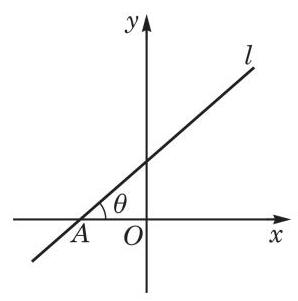
\includegraphics[max width=0.2\textwidth]{images/bo_d7fqvdc91nqc7381i9u0_8_198_628_298_301_0.jpg}
\end{center}
\hspace*{3em} 

图 1-1-1

如果知道了直线 \(l\) 的倾斜角以及它经过的一个确定的点,那么就准确地给出了直线 \(l\) 在坐标系中的位置. 由于倾斜角难以直接用坐标表示出来, 而倾斜角的三角函数与坐标的关系更为密切. 为此,我们引进一个新的概念: 当直线 \(l\) 的倾斜角 \(\theta  \neq  \frac{\pi }{2}\) 时, 定义 \(\tan \theta\) 为直线 \(l\) 的斜率 (slope),常用字母 \(k\) 表示,即 \(k = \tan \theta\) ; 当 \(\theta  = \frac{\pi }{2}\) ,即 \(l\) 与 \(x\) 轴垂直时,我们说直线 \(l\) 的斜率不存在.

我们来看如何用坐标表示一条直线的斜率.

设直线 \(l\) 经过不同的两点 \(A\left( {{x}_{1},{y}_{1}}\right) \text{ 、 }B\left( {{x}_{2},{y}_{2}}\right)\) . 当 \({x}_{1} = {x}_{2}\) 时,直线 \(l\) 与 \(x\) 轴垂直 (图 1-1-2),此时,直线 \(l\) 的倾斜角 \(\theta  = \frac{\pi }{2}\) , 斜率不存在.

\begin{center}
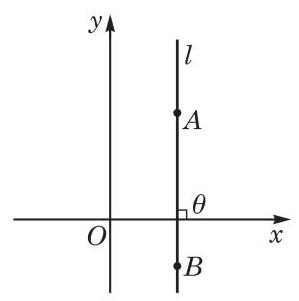
\includegraphics[max width=0.2\textwidth]{images/bo_d7fqvdc91nqc7381i9u0_8_554_1796_299_301_0.jpg}
\end{center}
\hspace*{3em} 

图 1-1-2

\begin{center}
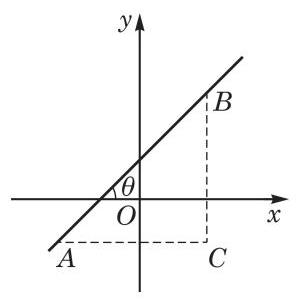
\includegraphics[max width=0.2\textwidth]{images/bo_d7fqvdc91nqc7381i9u0_8_872_1790_296_301_0.jpg}
\end{center}
\hspace*{3em} 

图 1-1-3

\begin{center}
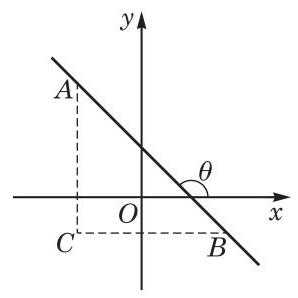
\includegraphics[max width=0.2\textwidth]{images/bo_d7fqvdc91nqc7381i9u0_8_1189_1792_298_298_0.jpg}
\end{center}
\hspace*{3em} 

图 1-1-4

当 \({x}_{1} \neq  {x}_{2}\) 时,不妨设 \({x}_{1} < {x}_{2}\) ,有以下 3 种情况:

(1)若 \({y}_{1} < {y}_{2}\) ，则 \(l\) 的倾斜角 \(\theta\) 为锐角. 如图 1-1-3，作直角三角形 \({ABC}\) ,可得 \(k = \frac{{y}_{2} - {y}_{1}}{{x}_{2} - {x}_{1}}\) .

(2)若 \({y}_{1} = {y}_{2}\) ，则直线 \(l\) 与 \(x\) 轴平行或重合，所以 \(l\) 的倾斜角 \(\theta  = 0\) ,斜率也等于 0,这就是 (1) 结果中令 \({y}_{1} = {y}_{2}\) 所得的值.

(3)若 \({y}_{1} > {y}_{2}\) ，则直线 \(l\) 的倾斜角 \(\theta\) 为钝角. 如图 1-1-4， 同样作直角三角形 \({ABC}\) ,则 \(\angle {ABC} = \pi  - \theta\) . 在直角三角形 \({ABC}\) 中,因为 \(\tan \angle {ABC} = \frac{\left| CA\right| }{\left| CB\right| } = \frac{{y}_{1} - {y}_{2}}{{x}_{2} - {x}_{1}}\) ,所以 \(\tan \left( {\pi  - \theta }\right)  = \; \frac{{y}_{1} - {y}_{2}}{{x}_{2} - {x}_{1}}\) ,由此得 \(\tan \theta  = \frac{{y}_{2} - {y}_{1}}{{x}_{2} - {x}_{1}}\) ,即 \(k = \frac{{y}_{2} - {y}_{1}}{{x}_{2} - {x}_{1}}\) ,这与(1)中的结果相同.

综上所述, 可以得到: 在平面直角坐标系中, 经过不同的两点 \(A\left( {{x}_{1},{y}_{1}}\right) \text{ 、 }B\left( {{x}_{2},{y}_{2}}\right) \left( {{x}_{1} \neq  {x}_{2}}\right)\) 的直线 \(l\) 的斜率为

\[
k = \frac{{y}_{2} - {y}_{1}}{{x}_{2} - {x}_{1}}.
\]

例 1 已知直线 \(l\) 经过点 \(A\left( {-1, - 1}\right) \text{ 、 }B\left( {2,3}\right)\) ,求它的斜率与倾斜角.

解 设直线 \(l\) 的斜率为 \(k\) ,倾斜角为 \(\theta\) ,则

\[
k = \tan \theta  = \frac{3 - \left( {-1}\right) }{2 - \left( {-1}\right) } = \frac{4}{3},
\]

从而 \(\theta  = \arctan \frac{4}{3}\) .

例 2 求一次函数 \(y = {kx} + b\left( {k \neq  0}\right)\) 所表示直线的斜率.

解 设一次函数 \(y = {kx} + b\left( {k \neq  0}\right)\) 的图像是直线 \(l\) . 在函数表达式中, \(x\) 的值分别取 \({x}_{1} = 0\) 及 \({x}_{2} = 1\) ,得 \({y}_{1} = b\) 及 \({y}_{2} = k + b\) . 所以, \(A\left( {0,b}\right)\) 与 \(B\left( {1,k + b}\right)\) 是直线 \(l\) 上的两点. 依据斜率公式, 得直线 \(l\) 的斜率为

\[
\frac{{y}_{2} - {y}_{1}}{{x}_{2} - {x}_{1}} = \frac{\left( {k + b}\right)  - b}{1 - 0} = k.
\]

例 3 已知三点 \(A\left( {-1,2}\right) \text{ 、 }B\left( {3,4}\right) \text{ 、 }C\left( {x,y}\right)\) 共线,求点 \(C\) 的坐标 \(x\) 与 \(y\) 所满足的关系式.

\HRule

一次函数 \(y = \; {kx} + b\left( {k \neq  0}\right)\) 的一次项系数 \(k\) 就是其对应直线的斜率.

\HRule

解 因为 \(A\text{ 、 }B\) 两点的横坐标不同,所以直线 \({AB}\) 的斜率是

\[
k = \frac{4 - 2}{3 - \left( {-1}\right) } = \frac{1}{2}.
\]

又由题设知,点 \(C\) 在直线 \({AB}\) 上,即 \({AB}\) 与 \({AC}\) 是同一条直线.

当点 \(C\) 与点 \(A\) 不重合时,用 \(A\text{ 、 }C\) 两点的坐标表示斜率得

\[
k = \frac{y - 2}{x - \left( {-1}\right) } = \frac{y - 2}{x + 1},
\]

此时 \(x\) 与 \(y\) 要满足的关系式是 \(\frac{y - 2}{x + 1} = \frac{1}{2}\) ,变形得

\[
y - 2 = \frac{1}{2}\left( {x + 1}\right) .
\]

当点 \(C\) 与点 \(A\) 重合时,点 \(C\) 的坐标也满足上式.

所以, \(x\) 与 \(y\) 满足的关系式是 \(y - 2 = \frac{1}{2}\left( {x + 1}\right)\) .

\section*{练习 1.1}

1. 求经过下列两点的直线的斜率和倾斜角:

(1) \(P\left( {-2,2}\right)\) 、 \(Q\left( {2, - 2}\right)\) ；

(2) \(P\left( {5,\sqrt{3}}\right)\) 、 \(Q\left( {2,2\sqrt{3}}\right)\) .

2. 在平面直角坐标系中有一个边长为 1 的正方形 \({OABC}\) ,其中 \(O\) 为坐标原点,点 \(A\) 、 \(C\) 分别在 \(x\) 轴和 \(y\) 轴上,点 \(B\) 在第一象限. 求直线 \({OB}\) 和 \({AC}\) 的斜率.

3. 证明: 在平面直角坐标系中, 如果两条直线平行, 那么它们的倾斜角相等.

\section*{习题 1.1}

\section*{A 组}

\begin{center}
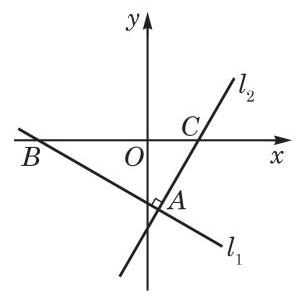
\includegraphics[max width=0.2\textwidth]{images/bo_d7fqvdc91nqc7381i9u0_10_1200_1802_298_298_0.jpg}
\end{center}
\hspace*{3em} 

(第 1 题)

1. 如图,在平面直角坐标系中,直线 \({l}_{1}\) 与 \({l}_{2}\) 垂直,垂足为 \(A\) , \({l}_{1}\text{ 、 }{l}_{2}\) 与 \(x\) 轴的交点分别为 \(B\text{ 、 }C,\angle {ABC} = \frac{\pi }{6}\) . 试分别求直线 \({l}_{1}\) 、 \({l}_{2}\) 的倾斜角和斜率.

2. 求经过下列两点的直线的斜率与倾斜角:

(1) \(P\left( {1,2}\right)\) 、 \(Q\left( {2, - 1}\right)\) ；

(2) \(M\left( {2,1}\right) \text{ 、 }N\left( {a, - 2}\right)\) ，其中实数 \(a\) 是常数.

3. 根据下列直线 \(l\) 的倾斜角 \(\theta\) 的取值范围,计算斜率 \(k\) 的取值范围:

(1) \(\theta  \in  \left\lbrack  {\frac{\pi }{4},\frac{\pi }{3}}\right\rbrack\) ；

\begin{center}
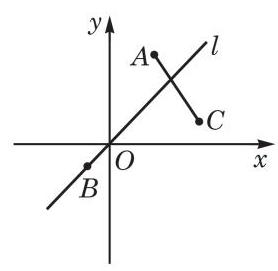
\includegraphics[max width=0.2\textwidth]{images/bo_d7fqvdc91nqc7381i9u0_11_1186_444_278_271_0.jpg}
\end{center}
\hspace*{3em} 

(第 5 题)

(2) \(\theta  \in  \left( {\frac{\pi }{2},\frac{2\pi }{3}}\right)\) .

4. 已知三个不同的点 \(A\left( {2,a}\right) \text{ 、 }B\left( {a + 1,{2a} + 1}\right) \text{ 、 }C\left( {-4,1 + a}\right)\) 在同一条直线上,求实数 \(a\) 的值及该直线的斜率.

5. 如图,已知点 \(A\left( {2,4}\right) \text{ 、 }B\left( {-1, - 1}\right) \text{ 、 }C\left( {4,1}\right)\) ,过点 \(B\) 的直线 \(l\) 与线段 \({AC}\) 相交. 求直线 \(l\) 的斜率 \(k\) 的取值范围.

\section*{B 组}

1. 已知常数 \(\theta  \in  \lbrack 0,\pi )\) ,试用 \(\theta\) 表示经过 \(P\left( {0,0}\right) \text{ 、 }Q\left( {\sin \theta ,\cos \theta }\right)\) 两点的直线 \(l\) 的倾斜角.

2. 设直线 \({l}_{1}\text{ 、 }{l}_{2}\) 的倾斜角分别为 \({\theta }_{1}\text{ 、 }{\theta }_{2}\) ,求证: \({l}_{1} \bot  {l}_{2}\) 的充要条件是 \(\left| {{\theta }_{1} - {\theta }_{2}}\right|  = \frac{\pi }{2}\) .

3. 已知直线 \(l\) 在平面直角坐标系中的斜率是 \(k\) ,向量 \(\overrightarrow{a}\) 在直线 \(l\) 上. 求向量 \(\overrightarrow{a}\) 在 \(x\) 轴上的投影向量.

\section*{1.2 直线的方程}

\section*{1 几种特殊形式的直线方程}

本章 1.1 节的例 3 中我们证明了与点 \(A\left( {-1,2}\right) \text{ 、 }B\left( {3,4}\right)\) 共线的点 \(C\left( {x,y}\right)\) 的坐标一定满足关系式 \(y - 2 = \frac{1}{2}\left( {x + 1}\right)\) . 反过来, 也容易验证: 如果点 \(C\left( {x,y}\right)\) 的坐标满足关系式 \(y - 2 = \frac{1}{2}\left( {x + 1}\right)\) , 那么点 \(C\left( {x,y}\right)\) 一定与点 \(A\left( {-1,2}\right) \text{ 、 }B\left( {3,4}\right)\) 共线. 这就是说, 经过点 \(A\left( {-1,2}\right) \text{ 、 }B\left( {3,4}\right)\) 的直线 \({AB}\) 上的点正好是以方程 \(y - 2 = \frac{1}{2}\left( {x + 1}\right)\) 的解作为坐标的点. 在这种情况下,我们说 “直线 \({AB}\) 的方程是 \(y - 2 = \frac{1}{2}\left( {x + 1}\right)\) ”,或者说 “方程 \(y - 2 = \frac{1}{2}\left( {x + 1}\right)\) 表示了直线 \({AB}\) ”. 可见,直线 \({AB}\) 的方程是一个关于 \(x\) 与 \(y\) 的二元一次方程. 本节中我们将看到,任何直线的方程都是关于 \(x\) 与 \(y\) 的二元一次方程,反过来,任何关于 \(x\) 与 \(y\) 的二元一次方程都表示一条直线. 而且, 这个方程实质上是唯一的, 即同一直线的不同方程通过简单变形可以互化. 然而, 不同形式的直线方程关注直线的不同几何要素, 在解决具体问题时也会有各自不同的作用.

\section*{(1)直线的点斜式方程}

如图 1-2-1,在平面直角坐标系中,设 \(P\left( {x,y}\right)\) 是过点 \(M\left( {{x}_{0},{y}_{0}}\right)\) 、斜率为 \(k\) 的直线 \(l\) 上的任意一点. 当点 \(P\left( {x,y}\right)\) 与点 \(M\) 不重合时,由 \(k = \frac{y - {y}_{0}}{x - {x}_{0}}\) ,可得

\begin{center}
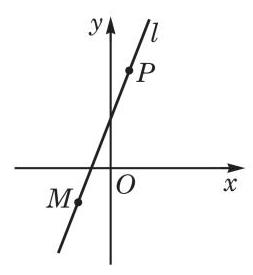
\includegraphics[max width=0.2\textwidth]{images/bo_d7fqvdc91nqc7381i9u0_12_220_1782_253_275_0.jpg}
\end{center}
\hspace*{3em} 

图 1-2-1

现在我们讨论, 在平面直角坐标系中, 当直线的斜率存在时,如何通过直线上的一个点 \(M\) 和直线的斜率 \(k\) 来求直线的方程.

\[
y - {y}_{0} = k\left( {x - {x}_{0}}\right) .
\]
  \circled{1} 

当点 \(P\left( {x,y}\right)\) 与点 \(M\) 重合时,点 \(P\) 的坐标就是 \(\left( {{x}_{0},{y}_{0}}\right)\) ,同样满足方程 \circled{1} . 这样,直线 \(l\) 上任意一点的坐标 \(\left( {x,y}\right)\) 都满足方程 \circled{1} .

反之,可以证明以方程 \circled{1} 的解为坐标的点一定在这条直线 \(l\) 上: 若点 \(Q\) 的坐标 \(\left( {{x}^{\prime },{y}^{\prime }}\right)\) 满足方程 \circled{1} ,即 \({y}^{\prime } - {y}_{0} = k\left( {{x}^{\prime } - {x}_{0}}\right)\) 成立. 当 \({x}^{\prime } \neq  {x}_{0}\) 时,直线 \({MQ}\) 经过点 \(M\) 且斜率 \({k}_{MQ} = \frac{{y}^{\prime } - {y}_{0}}{{x}^{\prime } - {x}_{0}} = k\) , 于是直线 \({MQ}\) 与 \(l\) 重合,从而点 \(Q\) 在 \(l\) 上; 当 \({x}^{\prime } = {x}_{0}\) 时,有 \({y}^{\prime } = {y}_{0}\) ,点 \(Q\) 与点 \(M\) 重合,点 \(Q\) 也在 \(l\) 上.

这就证明了方程 \circled{1} 是经过定点 \(M\left( {{x}_{0},{y}_{0}}\right)\) 且斜率为 \(k\) 的直线的方程. 这种形式的直线方程叫做直线的点斜式方程.

\HRule

本章 1.1 节中例 3 得到的方程就是一个点斜式方程.

\HRule

在点斜式方程 \circled{1} 中，如果把定点选成直线与 \(y\) 轴的交点 \(\left( {0,b}\right)\) ,那么方程改写为

\[
y = {kx} + b.
\]
  \circled{2} 

\begin{center}
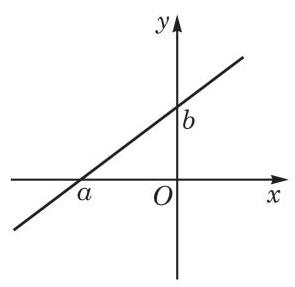
\includegraphics[max width=0.2\textwidth]{images/bo_d7fqvdc91nqc7381i9u0_13_1154_1266_295_287_0.jpg}
\end{center}
\hspace*{3em} 

图 1-2-2

其中，数值 \(b\) 称为该直线在 \(y\) 轴上的截距(图1-2-2). 当然，直线在 \(y\) 轴上的截距本质上是确定了直线上的一点 \(\left( {0,b}\right)\) ,所以给定直线的斜率和在 \(y\) 轴的截距,就唯一地确定了这条直线.

方程 \circled{2} 称为直线的斜截式方程. 当 \(k \neq  0\) 时,它表示 \(y\) 是 \(x\) 的一次函数,这个函数图像也就是我们所讨论的直线. 当 \(k = 0\) 时,该直线与 \(x\) 轴平行或重合,其方程为 \(y = b\) .

我们也可以定义直线在 \(x\) 轴上的截距,它就是直线与 \(x\) 轴交点 \(\left( {a,0}\right)\) 的横坐标 \(a\) (图 1-2-2).

如果直线与 \(y\) 轴平行或重合,它的斜率与在 \(y\) 轴上的截距都不存在,但此时直线与 \(x\) 轴垂直,设垂足为 \(\left( {a,0}\right)\) ,那么该直线在 \(x\) 轴上的截距为 \(a\) ,且直线上所有点的横坐标都是 \(a\) ,从而直线的方程是 \(x = a\) .

例 1 求倾斜角是 \(\frac{2\pi }{3}\) 且在 \(x\) 轴上的截距是 -3 的直线 \(l\) 的点斜式方程.

解 因为 \(l\) 在 \(x\) 轴上的截距是 -3,所以 \(l\) 经过点 \(A\left( {-3,0}\right)\) . 因为 \(l\) 的斜率 \(k = \tan \frac{2\pi }{3} =  - \sqrt{3}\) ,所以 \(l\) 的点斜式方程是 \(y = \; - \sqrt{3}\left( {x + 3}\right)\) .

例 2 已知直线 \(l\) 在 \(x\) 轴、 \(y\) 轴上的截距分别为 -2、 4, 求直线 \(l\) 的方程,并判断点 \(A\left( {2,6}\right)\) 是否在直线 \(l\) 上.

解 因为 \(l\) 在 \(y\) 轴上的截距是 4 且斜率 \(k\) 存在,所以可设 \(l\) 的方程为 \(y = {kx} + 4\) . 又因为 \(l\) 经过点 \(\left( {-2,0}\right)\) ,所以 \(- {2k} + 4 = 0\) , 解得 \(k = 2\) .

所以, \(l\) 的方程为 \(y = {2x} + 4\) .

因为 \(6 \neq  2 \times  2 + 4\) ,所以点 \(A\left( {2,6}\right)\) 不在直线 \(l\) 上.

\section*{练习 1.2(1)}

1. 求经过点 \(P\left( {-2,3}\right)\) 且斜率为 -1 的直线 \(l\) 的点斜式方程.

2. 求倾斜角是 \(\frac{5\pi }{6}\) 且在 \(x\) 轴上的截距为 -1 的直线 \(l\) 的点斜式方程.

3. 求经过点 \(A\left( {2,3}\right)\) 且垂直于 \(x\) 轴的直线 \(l\) 的方程.

4. 已知直线 \(l\) 经过点 \(M\left( {-2, - 1}\right)\) 且在 \(x\) 轴、 \(y\) 轴上截距相等,求 \(l\) 的方程.

\section*{(2) 直线的两点式方程}

两点确定一条直线, 因此, 只要给定平面上两个点的坐标, 就可以写出过这两点的直线的方程. 如果两点的横坐标或纵坐标相同, 那么这条直线与某条坐标轴平行或重合, 这种情况前面已经讨论过了.

现在考虑经过两点 \(M\left( {{x}_{1},{y}_{1}}\right) \text{ 、 }N\left( {{x}_{2},{y}_{2}}\right)\) ,并且不与任一坐标轴平行或重合的直线 \(l\) ,可知 \({x}_{1} \neq  {x}_{2}\) ,且 \({y}_{1} \neq  {y}_{2}\) ,直线 \(l\) 的斜率是 \(k = \frac{{y}_{2} - {y}_{1}}{{x}_{2} - {x}_{1}}\) ,于是该直线的点斜式方程为 \(y - {y}_{1} = \frac{{y}_{2} - {y}_{1}}{{x}_{2} - {x}_{1}}\left( {x - {x}_{1}}\right)\) , 整理成关于两个坐标对称的形式, 得 Q

\HRule

这就是本章 1.1 节中例 3 的解题过程.

\HRule

Q

\[
\frac{y - {y}_{1}}{{y}_{2} - {y}_{1}} = \frac{x - {x}_{1}}{{x}_{2} - {x}_{1}}.
\]
  \circled{3} 

\HRule

直线的两点式方程也可以写成

\(\left( {{x}_{2} - {x}_{1}}\right) \left( {y - {y}_{1}}\right)  = \; \left( {{y}_{2} - {y}_{1}}\right) \left( {x - {x}_{1}}\right)\) .

它对直线平行或重合于坐标轴的情形也适用.

\HRule

方程 \circled{3} 称为直线的两点式方程.

例 3 已知直线 \(l\) 经过点 \(A\left( {2,1}\right) \text{ 、 }B\left( {4,4}\right)\) ,求 \(l\) 的方程.

解 直接把点 \(A\text{ 、 }B\) 的坐标代入直线的两点式方程,得

\[
\frac{y - 1}{4 - 1} = \frac{x - 2}{4 - 2}
\]

化简, \(l\) 的方程可写为 \(y = \frac{3}{2}x - 2\) .

\begin{center}
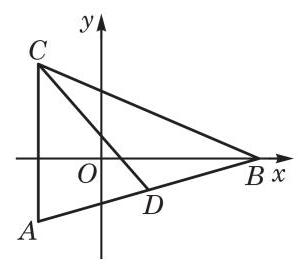
\includegraphics[max width=0.2\textwidth]{images/bo_d7fqvdc91nqc7381i9u0_15_1149_488_298_266_0.jpg}
\end{center}
\hspace*{3em} 

图 1-2-3

例 4 如图 1-2-3, \(\bigtriangleup {ABC}\) 三个顶点的坐标分别为 \(A\left( {-2, - 2}\right) \text{ 、 }B\left( {5,0}\right) \text{ 、 }C\left( {-2,3}\right)\) . 分别求边 \({AC}\) 所在直线的方程与边 \({AB}\) 上的中线 \({CD}\) 所在直线的方程.

解 因为点 \(A\) 与点 \(C\) 的横坐标相等,所以 \({AC}\) 所在直线与 \(x\) 轴垂直,从而边 \({AC}\) 所在直线的方程为 \(x =  - 2\) .

设点 \(D\) 的坐标为 \(\left( {{x}_{0},{y}_{0}}\right)\) ,则 \(\left\{  \begin{array}{l} {x}_{0} = \frac{-2 + 5}{2} = \frac{3}{2}, \\  {y}_{0} = \frac{-2 + 0}{2} =  - 1. \end{array}\right.\) 所以, 点 \(D\) 的坐标为 \(\left( {\frac{3}{2}, - 1}\right)\) .

又因为点 \(C\) 的坐标为 \(\left( {-2,3}\right)\) ,所以 \({CD}\) 所在直线的两点式方程是 \(\frac{y - 3}{-1 - 3} = \frac{x + 2}{\frac{3}{2} + 2}\) ,化简,得 \(y =  - \frac{8}{7}x + \frac{5}{7}\) .

所以, \(\bigtriangleup {ABC}\) 中边 \({AB}\) 上的中线 \({CD}\) 所在直线的方程为 \(y =  - \frac{8}{7}x + \frac{5}{7}.\)

例 5 已知直线 \(l\) 与 \(x\) 轴、 \(y\) 轴分别交于 \(A\) 、 \(B\) 两个不同的点且 \(\left| {OA}\right|  = \left| {OB}\right|\) ,其中 \(O\) 是坐标原点; 又点 \(C\left( {1, - 2}\right)\) 在直线 \(l\) 上. 求直线 \(l\) 的方程.

解 设 \(A\text{ 、 }B\) 两点的坐标分别为 \(\left( {a,0}\right) \text{ 、 }\left( {0,b}\right)\) . 因为 \(\left| {OA}\right|  = \; \left| {OB}\right|\) ,所以 \(b =  \pm  a\) 且 \(a \neq  0\) .

当 \(b = a\) 时,直线 \(l\) 的方程为 \(\frac{y - 0}{a - 0} = \frac{x - a}{0 - a}\) ,即 \(y =  - \left( {x - a}\right)\) .

因为点 \(C\left( {1, - 2}\right)\) 在直线 \(l\) 上,所以 \(- 2 =  - \left( {1 - a}\right)\) ,得 \(a =  - 1\) . 所以,直线 \(l\) 的方程为 \(y =  - x - 1\) .

同理,当 \(b =  - a\) 时,可得直线 \(l\) 的方程为 \(y = x - 3\) .

所以,直线 \(l\) 的方程为 \(y =  - x - 1\) 或 \(y = x - 3\) .

\section*{练习 1.2(2)}

1. 求经过点 \(A\left( {-2,3}\right) \text{ 、 }B\left( {0,6}\right)\) 的直线 \(l\) 的两点式方程.

2. 已知三个不同的点 \(A\left( {3,1}\right) \text{ 、 }B\left( {a + 1,3}\right) \text{ 、 }C\left( {{2a} - 1,3 - a}\right)\) 都在一条直线 \(l\) 上,求实数 \(a\) 的值和直线 \(l\) 的方程.

3. 在平面直角坐标系中, \(O\) 是坐标原点. 已知 \(A\text{ 、 }B\) 两点的坐标分别为 \(\left( {4,0}\right)\) 、 \(\left( {0,3}\right)\) ,分别求 \(\bigtriangleup {ABO}\) 的三条边上的中线所在直线的方程.

\section*{2 直线的一般式方程}

由前面的讨论可以看到,不管哪种形式的直线方程都是关于 \(x\) 、 \(y\) 的二元一次方程,因此都可以化为如下二元一次方程的一般形式

\[
{ax} + {by} + c = 0\text{ ( }a\text{ 、 }b\text{ 不同时为零). }
\]
  \circled{4} 

反过来, 二元一次方程 \circled{4} 是否都表示一条直线呢?

若 \(b \neq  0\) ,方程 \circled{4} 化为 \(y =  - \frac{a}{b}x - \frac{c}{b}\) ,它表示斜率为 \(- \frac{a}{b}\) , 在 \(y\) 轴上的截距为 \(- \frac{c}{b}\) 的直线; 若 \(b = 0\) ,则 \(a \neq  0\) ,方程 \circled{4} 化为 \(x =  - \frac{c}{a}\) ,它表示过点 \(\left( {-\frac{c}{a},0}\right)\) 且与 \(x\) 轴垂直的直线. 可见,只要 \(a\text{ 、 }b\) 不同时为零,方程 \circled{4} 都表示平面直角坐标系中的一条直线. 我们把方程 \circled{4} 称为直线的一般式方程.

例 6 在平面直角坐标系中, 根据所给直线方程, 作出相应图形，并求出该直线的斜率和在 \(y\) 轴上的截距:

(1) \({l}_{1} : {2y} + 1 = 0\) ;

\begin{center}
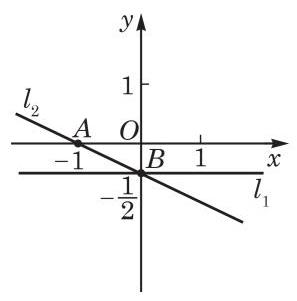
\includegraphics[max width=0.2\textwidth]{images/bo_d7fqvdc91nqc7381i9u0_16_200_1754_297_301_0.jpg}
\end{center}
\hspace*{3em} 

图 1-2-4

(2) \({l}_{2} : x + {2y} + 1 = 0\) .

解 (1) 因为 \({l}_{1} : y =  - \frac{1}{2}\) ,所以该直线过点 \(B\left( {0, - \frac{1}{2}}\right)\) 且平行于 \(x\) 轴 (图 1-2-4). 所以, \({l}_{1}\) 的斜率为 0 且在 \(y\) 轴上的截距是 \(- \frac{1}{2}\) .

(2)在方程 \(x + {2y} + 1 = 0\) 中，令 \(y = 0\) ，得 \(x =  - 1\) ；令 \(x = 0\) ， 得 \(y =  - \frac{1}{2}\) . 这就得到直线 \({l}_{2}\) 上两个不同的点 \(A\left( {-1,0}\right)\) 、 \(B\left( {0, - \frac{1}{2}}\right)\) ， 连接 \(A\text{ 、 }B\) 两点的直线即为直线 \({l}_{2}\) (图 1-2-4).

因为方程 \(x + {2y} + 1 = 0\) 可化为 \(y =  - \frac{1}{2}x - \frac{1}{2}\) ,所以直线 \({l}_{2}\) 的斜率是 \(- \frac{1}{2}\) ,在 \(y\) 轴上的截距是 \(- \frac{1}{2}\) .

例 7 已知直线 \(l\) 的方程为 \({ax} + y + a + 1 = 0\left( {a \in  \mathbf{R}}\right)\) ,求证: 无论 \(a\) 取何值时,直线 \(l\) 都经过一个定点,并写出该定点的坐标.

解 由 \({ax} + y + a + 1 = 0\) ,变形得 \(y + 1 =  - a\left( {x + 1}\right)\) . 这是直线 \(l\) 的点斜式方程, \(- a\) 是 \(l\) 的斜率,点 \(\left( {-1, - 1}\right)\) 是 \(l\) 经过的定点.

所以，无论 \(a\) 取何值时，直线 \(l\) 都经过一个定点，该定点的坐标为 \(\left( {-1, - 1}\right)\) .

\begin{center}
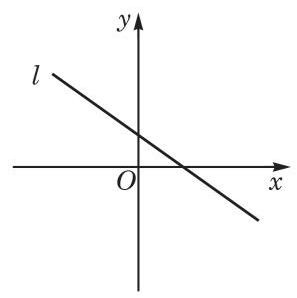
\includegraphics[max width=0.2\textwidth]{images/bo_d7fqvdc91nqc7381i9u0_17_1152_905_297_298_0.jpg}
\end{center}
\hspace*{3em} 

图 1-2-5

例 8 如图 1-2-5,直线 \(l : \left( {m + 1}\right) x + {my} + 2 - m = 0\) 经过平面直角坐标系的第一、第二与第四象限. 求实数 \(m\) 的取值范围.

解 当 \(m = 0\) 时,直线 \(l\) 的方程为 \(x =  - 2\) ,它只经过第二、 第三象限，不符题意，所以 \(m \neq  0\) . 于是，直线 \(l\) 的方程可化为

\[
y =  - \frac{m + 1}{m}x + \frac{m - 2}{m}.
\]

因为直线 \(l\) 经过第一、第二与第四象限,所以其斜率小于 0, 且在 \(y\) 轴上的截距大于 0,则

\[
\left\{  \begin{array}{l}  - \frac{m + 1}{m} < 0, \\  \frac{m - 2}{m} > 0, \end{array}\right.
\]

解得 \(m <  - 1\) 或 \(m > 2\) .

所以，实数 \(m\) 的取值范围是 \(\left( {-\infty , - 1}\right)  \cup  \left( {2, + \infty }\right)\) .

\section*{练习 1.2(3)}

1. 求下列方程所表示直线的斜率与倾斜角:

(1) \(x = 1\) ； (2) \(x + y - 1 = 0\) ；

(3) \(x + {2y} - 1 = 0\) ； (4) \(y = 1\) .

2. 求证: 无论实数 \(m\) 取何值,直线 \(l : x + \left( {m + 1}\right) y + 1 = 0\) 都经过一个定点.

3. 已知直线 \(l : {kx} + {2y} + 3 - k = 0\) 经过平面直角坐标系的第二、第三与第四象限，求实数 \(k\) 的取值范围.

例 9 已知点 \(A\left( {{x}_{1},{y}_{1}}\right)\) 与 \(B\left( {{x}_{2},{y}_{2}}\right)\) 是直线 \(l : {ax} + {by} + c = 0\) ( \(a\text{ 、 }b\) 不同时为零) 上任意两点,且向量 \(\overrightarrow{n} = \left( {a,b}\right)\) . 求证: 向量 \(\overrightarrow{n}\) 与 \(\overrightarrow{AB}\) 垂直.

证明 因为点 \(A\left( {{x}_{1},{y}_{1}}\right)\) 与 \(B\left( {{x}_{2},{y}_{2}}\right)\) 在直线 \(l\) 上,所以 \(a{x}_{1} + \; b{y}_{1} + c = 0\) 且 \(a{x}_{2} + b{y}_{2} + c = 0\) . 两式相减,得 \(a\left( {{x}_{2} - {x}_{1}}\right)  + \; b\left( {{y}_{2} - {y}_{1}}\right)  = 0\) ,即 \(\overrightarrow{n} \cdot  \overrightarrow{AB} = 0\) ,所以向量 \(\overrightarrow{n}\) 与 \(\overrightarrow{AB}\) 垂直.

例 9 中的向量 \(\overrightarrow{n} = \left( {a,b}\right)\) 与直线 \(l\) 上的任意一个向量都垂直. 一般地，与直线上任意一个向量都垂直的非零向量叫做该直线的法向量(normal vector). 于是，例 9 可以总结为如下结论:

以直线 \(l\) 的一般式方程 \({ax} + {by} + c = 0\) ( \(a\) 、 \(b\) 不同时为零)的一次项系数为坐标的向量 \(\overrightarrow{n} = \left( {a,b}\right)\) 是 \(l\) 的一个法向量.

如果知道了直线 \(l\) 上的一个点 \(M\left( {{x}_{0},{y}_{0}}\right)\) 和 \(l\) 的一个法向量 \(\overrightarrow{n} = \left( {a,b}\right)\) ,那么平面上一点 \(P\left( {x,y}\right)\) 在直线 \(l\) 上的充要条件是 \(\overrightarrow{n} \bot  \overrightarrow{MP}\) ,或用向量数量积写成 \(\overrightarrow{n} \cdot  \overrightarrow{MP} = 0\) . 因为向量 \(\overrightarrow{MP} = \; \left( {x - {x}_{0},y - {y}_{0}}\right)\) ,所以平面上一点 \(P\left( {x,y}\right)\) 在直线 \(l\) 上的充要条件变成了

\[
a\left( {x - {x}_{0}}\right)  + b\left( {y - {y}_{0}}\right)  = 0.
\]
  \circled{5} 

这又给出了直线 \(l\) 的一个方程,这个方程称为直线的点法式方程, 它是一个几何意义明确、没有任何附加限制条件的直线方程. 只要令 \(c =  - a{x}_{0} - b{y}_{0}\) ,直线的点法式方程 \circled{5} 就化归为一般式方程 \circled{4} 了.

例 10 已知 \(\bigtriangleup {ABC}\) 的三个顶点的坐标分别是 \(A\left( {1,6}\right)\) 、 \(B\left( {-1, - 2}\right)\) 与 \(C\left( {6,3}\right)\) ,求边 \({BC}\) 上的高 \({AD}\) 所在直线的方程.

解 因为 \({AD} \bot  {BC}\) ,所以向量 \(\overrightarrow{BC} = \left( {7,5}\right)\) 是 \({AD}\) 所在直线的一个法向量; 又因为直线 \({AD}\) 经过点 \(A\left( {1,6}\right)\) ,所以 \({AD}\) 所在直线的点法式方程是 \(7\left( {x - 1}\right)  + 5\left( {y - 6}\right)  = 0\) .

化简,得 \(\bigtriangleup {ABC}\) 的高 \({AD}\) 所在直线的方程为 \({7x} + {5y} - {37} = 0\) .

例 11 已知直线 \(l\) 经过点 \(P\left( {3,2}\right)\) ，且 \(\overrightarrow{n} = \left( {m,1 - m}\right)\) 是它的一个法向量. 若 \(l\) 与坐标轴围成的三角形的面积是 2,求实数 \(m\) 的值.

\HRule

如果 \(\overrightarrow{n} = \left( {a,b}\right)\) 是直线 \(l\) 的一个法向量， 那么,只要 \(k\) 是非零实数, \(k\overrightarrow{n} = \left( {{ka},{kb}}\right)\) 也是 \(l\) 的法向量.

\HRule

解 根据条件写出直线 \(l\) 的点法式方程

\[
m\left( {x - 3}\right)  + \left( {1 - m}\right) \left( {y - 2}\right)  = 0.
\]

化简为

\[
{mx} + \left( {1 - m}\right) y - m - 2 = 0.
\]

如果 \(m = 0\) 或 \(m = 1\) ,直线 \(l\) 与 \(x\) 轴或 \(y\) 轴平行,这样的直线无法与坐标轴围成三角形,所以 \(m \neq  0\) 且 \(m \neq  1\) .

在上述方程中分别令 \(y\) 与 \(x\) 等于零,求得直线 \(l\) 在 \(x\) 轴与 \(y\) 轴上的截距分别是 \(\frac{m + 2}{m}\) 与 \(\frac{m + 2}{1 - m}\) . 所以, \(l\) 与坐标轴围成的三角形的面积为

\[
\frac{1}{2} \times  \left| \frac{m + 2}{m}\right|  \times  \left| \frac{m + 2}{1 - m}\right|  = 2,
\]

解得 \(m = \frac{4 + 2\sqrt{7}}{3}\) 或 \(m = \frac{4 - 2\sqrt{7}}{3}\) .

\section*{练习 1.2(4)}

1. 写出下列直线的一个法向量:

(1) \({2x} - {3y} + 1 = 0\) ； (2) \({3x} + {2y} + 1 = 0\) ；

(3) \(x + 3 = 0\) ；

(4) \(y = \frac{1}{2}x - 3\) .

2. 已知直线 \(l\) 的方程是 \(\left( {a - 3}\right) x + \left( {{2a} + 1}\right) y - 3 = 0\) ,它的一个法向量是 \(\overrightarrow{n} = \left( {3,2}\right)\) . 求实数 \(a\) 的值.

3. 根据下列条件,求直线 \(l\) 的方程:

(1) \(l\) 在 \(x\) 轴上的截距为 -1，且 \(l\) 的一个法向量是 \(\overrightarrow{n} = \left( {-1,2}\right)\) ；

(2) \(l\) 经过点 \(\left( {2,3}\right)\) ，且 \(l\) 上的任何向量都与向量 \(\overrightarrow{a} = \left( {1,2}\right)\) 平行.

\section*{习题 1.2}

\section*{A 组}

1. 已知直线 \(l\) 经过点 \(P\left( {3,5}\right)\) ，倾斜角为 \(\alpha\) 且 \(\cos \alpha  = \frac{3}{5}\) . 求直线 \(l\) 的点斜式方程.

2. 已知直线 \(l\) 在 \(y\) 轴上的截距为 4,倾斜角为 \(\alpha\) 且 \(\sin \alpha  = \frac{3}{5}\) . 求直线 \(l\) 的斜截式方程.

3. 求下列直线的斜率与在 \(x\text{ 、 }y\) 两坐标轴上的截距:

(1) \({l}_{1} : {y + 1} =  - \frac{\sqrt{3}}{3}\left( {x + 1}\right)\) ；

(2) \({l}_{2} : y =  - {3x} + \sqrt{3}\) .

4. 已知直线 \(l : y = {kx} + 2\) 经过点 \(\left( {1, - 3}\right)\) .

(1)求 \(l\) 的倾斜角的大小；

(2)求 \(l\) 在 \(x\) 轴上的截距.

5. 直线 \(l\) 经过点 \(P\left( {-2,1}\right)\) ,在 \(x\) 轴、 \(y\) 轴上的截距分别为 \(a\text{ 、 }b\) . 已知 \(a + b = 4\) ,求直线 \(l\) 的方程.

6. 根据给定条件,求下列直线的两点式方程:

(1)直线 \({l}_{1}\) 经过点 \(A\left( {2,0}\right)\) 、 \(B\left( {3,7}\right)\) ；

(2)直线 \({l}_{2}\) 与坐标轴的交点分别为 \(\left( {3,0}\right) \text{ 、 }\left( {0, - 1}\right)\) .

7. 已知 \(\bigtriangleup  {ABC}\) 的三个顶点的坐标分别为 \(A\left( {3,8}\right)\) 、 \(B\left( {3, - 2}\right)\) 、 \(C\left( {-3,0}\right)\) .

(1)求边 \({BC}\) 所在直线的方程；

(2)求边 \({BC}\) 上的中线所在直线的方程.

8. 设直线 \(l\) 在 \(x\) 轴与 \(y\) 轴上的截距分别是 \(a\) 与 \(b\) ,且 \(a\) 与 \(b\) 均不为零. 求证: 直线 \(l\) 的方程可以写成 \(\frac{x}{a} + \frac{y}{b} = 1\) .

9. 一个弹簧在弹性限度内挂 \(4\mathrm{\;{kg}}\) 的物体时弹簧长度为 \({20}\mathrm{\;{cm}}\) ,挂 \(5\mathrm{\;{kg}}\) 物体时弹簧长度为 \({21.5}\mathrm{\;{cm}}\) . 已知在弹性限度内所挂物体的质量 \(x\) (单位: \(\mathrm{{kg}}\) )与弹簧长度 \(y\) (单位: \(\mathrm{{cm}}\) ) 的关系可以用直线的方程表示, 求该直线的方程, 并求弹簧自身的长度.

10. 在平面直角坐标系中, 作出下列直线, 并求它们的斜率与倾斜角.

(1) \({l}_{1} : {3x} - y - 2 = 0\) ；

(2) \({l}_{2} : {3x} + {2y} - 1 = 0\) .

11. 设直线 \(l\) 的方程是 \({ax} + {by} + c = 0\) ,在下列条件下,求实数 \(a\text{ 、 }b\text{ 、 }c\) 满足的条件:

(1) \(l\) 与 \(x\) 轴、 \(y\) 轴均相交；

(2) \(l\) 经过第二、第三、第四象限.

12. 已知直线 \(l : {ax} + \left( {4 - {2a}}\right) y - 3 = 0\) ，根据下列条件，求实数 \(a\) 的值:

(1) \(l\) 经过点 \(\left( {1,1}\right)\) ；

(2) \(l\) 在两个坐标轴上的截距相等.

13. 已知 \(A\left( {7, - 4}\right) \text{ 、 }B\left( {-5,6}\right)\) 两点,求线段 \({AB}\) 的垂直平分线的点法式方程.

14. 已知直线 \({l}_{1} : {3kx} + \left( {k + 2}\right) y + 6 = 0\) ，直线 \({l}_{2} : {kx} + \left( {{2k} - 3}\right) y + 2 = 0\) . 若这两条直线的法向量互相垂直,求 \(k\) 的值.

B 组

1. 已知平行四边形 \({ABCD}\) 中,三个顶点的坐标分别为 \(A\left( {1,2}\right) \text{ 、 }B\left( {3,4}\right) \text{ 、 }C\left( {2,6}\right)\) . 分别求边 \({AD}\text{ 、 }{CD}\) 所在直线的方程.

2. 已知直线 \(l\) 经过点 \(P\left( {2, - 1}\right)\) ，与 \(x\) 轴、 \(y\) 轴分别交于 \(A\) 、 \(B\) 两点. 若 \(2\overrightarrow{PA} + \overrightarrow{PB} = \; \overrightarrow{0}\) ,求直线 \(l\) 的方程.

3. 直线 \(l : y = {kx} + b\left( {k\text{ 、 }b \in  \mathbf{R}}\right)\) 与线段 \({AB}\) 相交，其中点 \(A\) 为 \(\left( {4,2}\right)\) ，点 \(B\) 为 \(\left( {1,5}\right)\) .

(1)当 \(b =  - 1\) 时，求 \(k\) 的取值范围;

(2)当 \(k = 1\) 时,求 \(b\) 的取值范围.

4. 已知 \(\bigtriangleup {ABC}\) 中,两个顶点的坐标分别为 \(A\left( {-2,1}\right) \text{ 、 }B\left( {4, - 3}\right)\) ,点 \(G\left( {0,2}\right)\) 是此三角形的重心. 求边 \({BC}\text{ 、 }{AC}\) 所在直线的方程.

5. 若 \(2{x}_{1} + 3{y}_{1} = 1,2{x}_{2} + 3{y}_{2} = 1\) ,且 \({x}_{1} \neq  {x}_{2}\) . 求经过两点 \(A\left( {x}_{1}\right.\) , \(\left. {y}_{1}\right) \text{ 、 }B\left( {{x}_{2},{y}_{2}}\right)\) 的直线 \(l\) 的方程.

\begin{center}

\includegraphics[max width=0.2\textwidth]{images/bo_d7fqvdc91nqc7381i9u0_21_1269_857_152_152_0.jpg}
\end{center}
\hspace*{3em} 

(第 6 题)

6. 如图是一个 W 形的霓虹灯 (灯管宽度忽略不计),每边长都是 \(2\mathrm{\;m}\) , 每相邻两边相交所成的锐角都是 \({30}^{ \circ  }\) . 试建立适当的平面直角坐标系, 写出此霓虹灯的每条边所在直线在这个坐标系中的方程.

7. 证明: 直线 \({2x} + \left( {1 - \cos {2\theta }}\right) y - \sin \theta  = 0\) ( \(\theta  \in  \mathbf{R}\) 且不是 \(\pi\) 的整数倍) 和两坐标轴围成图形的面积是定值.

8. 已知直线 \(l : \left( {a - 1}\right) x + \left( {3 - {2a}}\right) y + a + 1 = 0\) .

(1)若直线的斜率 \(k \in  \left\lbrack  {-1,2}\right\rbrack\) ，求实数 \(a\) 的取值范围；

(2)求证:对任意实数 \(a\) ，直线 \(l\) 都经过一个定点.

9. 已知向量 \(\overrightarrow{n} = \left( {5, - 1}\right)\) 是直线 \(l\) 的一个法向量，在下列条件下求直线 \(l\) 的方程:

(1)在 \(x\) 轴、 \(y\) 轴上的截距之和为 4 ；

(2)与 \(x\) 轴、 \(y\) 轴围成的三角形面积为 20.

10. 已知 \(\overrightarrow{n} = \left( {a,b}\right)\) (其中 \({ab} \neq  0\) ) 是直线 \(l\) 的一个法向量,试用 \(a\text{ 、 }b\) 表示直线 \(l\) 的倾斜角.

11. 我们把与直线上任意两点构成的向量均平行的非零向量称为该直线的方向向量. 求经过点 \(P\left( {{x}_{0},{y}_{0}}\right)\) 且以 \(\overrightarrow{d} = \left( {u,v}\right)\) 为方向向量的直线的方程.

\section*{1.3 两条直线的位置关系}

\section*{1 两条直线的相交、平行与重合}

在平面几何中, 可依据公共点的个数判定两条直线的三种位置关系: 如果两条直线无公共点, 那么这两条直线平行; 如果两条直线有且只有一个公共点, 那么这两条直线相交; 如果两条直线至少有两个不同的公共点, 那么这两条直线重合为一条直线, 即有无穷多个公共点. 但用平面几何方法来判断两条直线是否有公共点、有多少个公共点, 有时候并不是一件容易的事.

在解析几何中, 我们可以将上述几何问题转化为代数问题来解决, 一般性的方法如下:

在平面直角坐标系中, 已知两条直线:

\({l}_{1} : {a}_{1}x + {b}_{1}y + {c}_{1} = 0\left( {{a}_{1}\text{ 、 }{b}_{1}\text{ 不同时为零 }}\right) , \; {l}_{2} : {a}_{2}x + {b}_{2}y + {c}_{2} = 0\left( {{a}_{2}\text{ 、 }{b}_{2}\text{ 不同时为零 }}\right) .\)

如果这两条直线有公共点 \(M\left( {{x}_{0},{y}_{0}}\right)\) ,那么点 \(M\left( {{x}_{0},{y}_{0}}\right)\) 的坐标要同时满足这两条直线的方程,即 \(\left\{  \begin{array}{l} x = {x}_{0}, \\  y = {y}_{0} \end{array}\right.\) 是方程组

\[
\left\{  \begin{array}{l} {a}_{1}x + {b}_{1}y + {c}_{1} = 0, \\  {a}_{2}x + {b}_{2}y + {c}_{2} = 0 \end{array}\right.
\]
  \circled{1} 

的解; 反过来,以方程组 \circled{1} 的解为坐标的点也必是 \({l}_{1}\) 与 \({l}_{2}\) 的公共点. 这样, 我们可以通过讨论方程组 \circled{1} 的解的情况来判断两条直线的位置关系.

方程组 \circled{1} 的解可分 3 种情况讨论:

(1)若存在 \(\lambda  \in  \mathbf{R}\) ,使得 \({a}_{1} = \lambda {a}_{2},{b}_{1} = \lambda {b}_{2}\) 且 \({c}_{1} = \lambda {c}_{2}\) ,则方程组 \circled{1} 的两个方程表示的是同一条直线，也就是说，直线 \({l}_{1}\) 与 \({l}_{2}\) 重合(此时方程组 \circled{1} 有无数组解);

(2)若存在 \(\lambda  \in  \mathbf{R}\) ,使得 \({a}_{1} = \lambda {a}_{2},{b}_{1} = \lambda {b}_{2}\) 但 \({c}_{1} \neq  \lambda {c}_{2}\) ,把第二个方程两边同乘 \(\lambda\) 后减去第一个方程,得到 \(\lambda {c}_{2} - {c}_{1} = 0\) ,这个等式不可能成立,则方程组 \circled{1} 无解,即直线 \({l}_{1}\) 与 \({l}_{2}\) 无公共点, 从而 \({l}_{1}//{l}_{2}\) ;

(3)若不存在 \(\lambda  \in  \mathbf{R}\) ,使得 \({a}_{1} = \lambda {a}_{2},{b}_{1} = \lambda {b}_{2}\) ,这个条件等价于 \({a}_{1}{b}_{2} \neq  {a}_{2}{b}_{1}\) ,此时可以求得方程组 \circled{1} 的唯一解

\[
\left\{  \begin{array}{l} x = \frac{{c}_{2}{b}_{1} - {c}_{1}{b}_{2}}{{a}_{1}{b}_{2} - {a}_{2}{b}_{1}}, \\  y = \frac{{c}_{1}{a}_{2} - {c}_{2}{a}_{1}}{{a}_{1}{b}_{2} - {a}_{2}{b}_{1}}, \end{array}\right.
\]

说明直线 \({l}_{1}\) 与 \({l}_{2}\) 有唯一的公共点,即 \({l}_{1}\) 与 \({l}_{2}\) 相交.

总结一下: 给定两条直线

\({l}_{1} : {a}_{1}x + {b}_{1}y + {c}_{1} = 0\left( {{a}_{1}\text{ 、 }{b}_{1}}\right.\) 不同时为零 \()\) ,

\({l}_{2} : {a}_{2}x + {b}_{2}y + {c}_{2} = 0\left( {{a}_{2}\text{ 、 }{b}_{2}\text{ 不同时为零 }}\right) ,\) 那么:

\({l}_{1}\) 与 \({l}_{2}\) 重合 \(\Leftrightarrow\) 存在 \(\lambda  \in  \mathbf{R}\) ,使得 \({a}_{1} = \lambda {a}_{2},{b}_{1} = \lambda {b}_{2}\) , 且 \({c}_{1} = \lambda {c}_{2}\) ;

\({l}_{1}//{l}_{2} \Leftrightarrow\) 存在 \(\lambda  \in  \mathbf{R}\) ,使得 \({a}_{1} = \lambda {a}_{2},{b}_{1} = \lambda {b}_{2}\) , 但 \({c}_{1} \neq  \lambda {c}_{2}\) ;

\({l}_{1}\) 与 \({l}_{2}\) 相交 \(\Leftrightarrow  {a}_{1}{b}_{2} \neq  {a}_{2}{b}_{1}\) .

如果 \({l}_{2}\) 的方程中三个系数 \({a}_{2}\text{ 、 }{b}_{2}\) 与 \({c}_{2}\) 均不为零,那么上述的充要条件可以写成更易于记忆的形式:

\({l}_{1}\) 与 \({l}_{2}\) 重合 \(\Leftrightarrow  \frac{{a}_{1}}{{a}_{2}} = \frac{{b}_{1}}{{b}_{2}} = \frac{{c}_{1}}{{c}_{2}}\) ; \({l}_{1}//{l}_{2} \Leftrightarrow  \frac{{a}_{1}}{{a}_{2}} = \frac{{b}_{1}}{{b}_{2}} \neq  \frac{{c}_{1}}{{c}_{2}}; \; {l}_{1}\) 与 \({l}_{2}\) 相交 \(\Leftrightarrow  \frac{{a}_{1}}{{a}_{2}} \neq  \frac{{b}_{1}}{{b}_{2}}\) .

还有其他一些量可以简单地刻画两条直线相交与否:

因为 \(\overrightarrow{{n}_{1}} = \left( {{a}_{1},{b}_{1}}\right)\) 与 \(\overrightarrow{{n}_{2}} = \left( {{a}_{2},{b}_{2}}\right)\) 分别是 \({l}_{1}\) 与 \({l}_{2}\) 的法向量, 所以上述第三个充要条件表明, \({l}_{1}\) 与 \({l}_{2}\) 相交的充要条件是它们的法向量不平行,从而 \({l}_{1}\) 与 \({l}_{2}\) 平行或重合的充要条件是它们的法向量平行 (这个结论也可以从另外两个充要条件得出).

如果 \({b}_{1}\) 与 \({b}_{2}\) 均不为零,那么容易求出 \({l}_{1}\) 与 \({l}_{2}\) 的斜率分别是 \({k}_{1} =  - \frac{{a}_{1}}{{b}_{1}}\) 与 \({k}_{2} =  - \frac{{a}_{2}}{{b}_{2}}\) ,上述第三个充要条件又可以表明, \({l}_{1}\) 与 \({l}_{2}\) 相交的充要条件是它们的斜率不相等,从而 \({l}_{1}\) 与 \({l}_{2}\) 平行或重合的充要条件是它们的斜率相等 (这也可以从另外两个充要条件得出).

用法向量或斜率表述的充要条件从几何上看也很直观.

例 1 判断下列两条直线的位置关系. 若相交, 求交点坐标.

(1) \({l}_{1} : {0.5x} - y + 1 = 0,{l}_{2} : {3x} - {6y} + 8 = 0\) ；

(2) \({l}_{1} : y = {2x} + 3,{l}_{2} : y =  - {2x} + 1.\)

解 (1) 因为 \(\frac{0.5}{3} = \frac{-1}{-6} \neq  \frac{1}{8}\) ,所以 \({l}_{1}//{l}_{2}\) .

(2)因为 \({l}_{1}\) 与 \({l}_{2}\) 的斜率分别为 \({k}_{1} = 2,{k}_{2} =  - 2\) ,则 \({k}_{1} \neq  {k}_{2}\) ， 所以两条直线相交.

解方程组 \(\left\{  \begin{array}{l} y = {2x} + 3, \\  y =  - {2x} + 1, \end{array}\right.\) 得 \(\left\{  \begin{array}{l} x =  - \frac{1}{2}, \\  y = 2. \end{array}\right.\)

所以，两条直线的交点坐标为 \(\left( {-\frac{1}{2},2}\right)\) .

例 2 已知直线 \({l}_{1} : {mx} - {2y} + 1 = 0,{l}_{2} : x - \left( {m + 1}\right) y + \; 1 = 0\) ,求实数 \(m\) 的取值范围,使得:

(1) \({l}_{1}\) 与 \({l}_{2}\) 相交;

(2) \({l}_{1}//{l}_{2}\) ；

(3) \({l}_{1}\) 与 \({l}_{2}\) 重合.

解 因为 \({l}_{1}\) 与 \({l}_{2}\) 相交的充要条件是 \(m\left\lbrack  {-\left( {m + 1}\right) }\right\rbrack   \neq  1 \times  \left( {-2}\right)\) , 所以先解方程 \(m\left\lbrack  {-\left( {m + 1}\right) }\right\rbrack   = 1 \times  \left( {-2}\right)\) ,得 \(m =  - 2\) 或 \(m = 1\) . 于是有:

(1)当 \(m \neq   - 2\) 且 \(m \neq  1\) 时， \({l}_{1}\) 与 \({l}_{2}\) 相交.

( 2 )当 \(m =  - 2\) 时，因为 \(\frac{1}{m} = \frac{-\left( {m + 1}\right) }{-2} \neq  \frac{1}{1}\) ，所以 \({l}_{1}//{l}_{2}\) .

(3)当 \(m = 1\) 时,因为 \(\frac{1}{m} = \frac{-\left( {m + 1}\right) }{-2} = \frac{1}{1}\) ,所以 \({l}_{1}\) 与 \({l}_{2}\) 重合.

\section*{练习 1.3(1)}

1. 判断下列两条直线的位置关系. 若相交, 求交点坐标.

(1) \({l}_{1} : x + {3y} + 1 = 0,{l}_{2} : {3x} + 4 = 0\) ;

(2) \({l}_{1} : x - {3y} + 1 = 0,{l}_{2} : y = \frac{1}{3}x + 4\) .

2. 已知直线 \({l}_{1} : \left( {a + 1}\right) x + y + a = 0,{l}_{2} : x + \left( {a + 1}\right) y - 2 = 0\) . 若 \({l}_{1}//{l}_{2}\) ，求实数 \(a\) 的值.

3. 求经过直线 \({l}_{1} : x - y - 4 = 0\) 与 \({l}_{2} : {2x} - {3y} - 7 = 0\) 的交点,且与直线 \({l}_{3} : {2x} + \; y + 1 = 0\) 平行的直线 \(l\) 的方程.

\section*{2 两条直线垂直的判定与夹角的求法}

我们已经知道, 平面上两条相交直线交得的锐角或直角叫做这两条直线的夹角. 当两条直线的夹角为直角时, 称这两条直线垂直.

在平面直角坐标系中, 给定两条相交的直线

\[
{l}_{1} : {a}_{1}x + {b}_{1}y + {c}_{1} = 0\left( {{a}_{1}\text{ 、 }{b}_{1}\text{ 不同时为零 }}\right) ,
\]

\[
{l}_{2} : {a}_{2}x + {b}_{2}y + {c}_{2} = 0\left( {{a}_{2}\text{ 、 }{b}_{2}\text{ 不同时为零 }}\right) .
\]

如何根据方程判定两条直线是否垂直呢?

\begin{center}
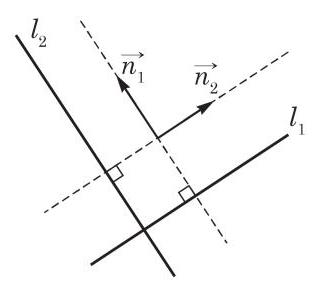
\includegraphics[max width=0.2\textwidth]{images/bo_d7fqvdc91nqc7381i9u0_25_1149_1200_312_287_0.jpg}
\end{center}
\hspace*{3em} 

图 1-3-1

我们知道, \(\overrightarrow{{n}_{1}} = \left( {{a}_{1},{b}_{1}}\right)\) 与 \(\overrightarrow{{n}_{2}} = \left( {{a}_{2},{b}_{2}}\right)\) 分别是直线 \({l}_{1}\) 与 \({l}_{2}\) 的法向量. 由于直线与其法向量所在直线垂直 (图 1-3-1), 因此 \({l}_{1} \bot  {l}_{2} \Leftrightarrow  \overrightarrow{{n}_{1}} \bot  \overrightarrow{{n}_{2}}\) ,再由必修课程 8.3 节的向量垂直的充要条件 \(\overrightarrow{{n}_{1}} \bot  \overrightarrow{{n}_{2}} \Leftrightarrow  {a}_{1}{a}_{2} + {b}_{1}{b}_{2} = 0\) ,我们得到

\[
{l}_{1} \bot  {l}_{2} \Leftrightarrow  {a}_{1}{a}_{2} + {b}_{1}{b}_{2} = 0.
\]

特别地,当 \({b}_{1}{b}_{2} \neq  0\) 时,直线 \({l}_{1}\) 与 \({l}_{2}\) 的斜率都存在,分别为 \({k}_{1} =  - \frac{{a}_{1}}{{b}_{1}}\) 与 \({k}_{2} =  - \frac{{a}_{2}}{{b}_{2}}\) ,条件 \({a}_{1}{a}_{2} + {b}_{1}{b}_{2} = 0\) 可以改写为 \(\frac{{a}_{1}}{{b}_{1}} \cdot  \frac{{a}_{2}}{{b}_{2}} =\) -1,即 \({k}_{1}{k}_{2} =  - 1\) . 于是

\[
{l}_{1} \bot  {l}_{2} \Leftrightarrow  {k}_{1}{k}_{2} =  - 1.
\]

例 3 已知直线 \({l}_{1} : x + {my} - 2 = 0\) 与 \({l}_{2} : \left( {m - 2}\right) x + \; {3my} + {2m} = 0\) 互相垂直，求实数 \(m\) 的值.

解 由两条直线互相垂直的充要条件, 得

\[
\left( {m - 2}\right)  + 3{m}^{2} = 0,
\]

解得

\[
m = \frac{2}{3}\text{ 或 }m =  - 1.
\]

例4 求经过点 \(\left( {4,5}\right)\) 且与直线 \(l : y =  - \frac{1}{3}x + 2\) 垂直的直线 \({l}^{\prime }\) 的方程.

解 因为 \(l\) 的斜率 \(k =  - \frac{1}{3}\) ,且 \(l \bot  {l}^{\prime }\) ,所以 \({l}^{\prime }\) 的斜率 \({k}^{\prime } = 3\) .

因为 \({l}^{\prime }\) 经过点 \(\left( {4,5}\right)\) ,所以 \({l}^{\prime }\) 的点斜式方程是 \(y - 5 = \; 3\left( {x - 4}\right)\) ,化简为 \({3x} - y - 7 = 0\) .

例 5 已知直角三角形 \({ABC}\) 的斜边 \({BC}\) 在 \(x\) 轴上，且长度为 8,直角顶点 \(A\) 的坐标是 \(\left( {2,4}\right)\) . 求直角边 \({AB}\) 所在直线的方程.

解 根据条件可知,直角边 \({AB}\) 斜率存在且不为零. 不妨设此斜率为 \(k\) ,则 \({AC}\) 所在直线的斜率为 \(- \frac{1}{k}\) . 所以 \({AB}\) 与 \({AC}\) 所在的直线方程分别为 \(y - 4 = k\left( {x - 2}\right)\) 与 \(y - 4 =  - \frac{1}{k}\left( {x - 2}\right)\) . 令 \(y = 0\) ,得点 \(B\) 与点 \(C\) 的横坐标分别为 \(2 - \frac{4}{k}\) 与 \(2 + {4k}\) .

由 \(\left| {BC}\right|  = 8\) ,得 \(\left| {{4k} + \frac{4}{k}}\right|  = 8\) ,解得 \(k = 1\) 或 \(k =  - 1\) .

所以,直角边 \({AB}\) 所在直线的方程为 \(y = x + 2\) 或 \(y =  - x + 6\) .

\section*{练习 1.3(2)}

1. 已知直线 \({l}_{1} : \left( {a - 2}\right) x + {ay} - 2 = 0\) 与 \({l}_{2} : \left( {1 - a}\right) x + \left( {a + 1}\right) y + 1 = 0\) 互相垂直， 求实数 \(a\) 的值.

2. 求过点 \(\left( {-1, - 1}\right)\) 且分别与下列直线垂直的直线方程:

(1) \(y = 2\) ；

(2) \(y = x\) ；

(3) \({2x} + y + 2 = 0\) ；

(4) \(x\cos \theta  + y\sin \theta  = 1,\theta\) 为给定的实数.

如果 \({l}_{1} : {a}_{1}x + {b}_{1}y + {c}_{1} = 0\) 与 \({l}_{2} : {a}_{2}x + {b}_{2}y + {c}_{2} = 0\) 是给定的两条相交直线,我们该如何求出它们的夹角 \(\alpha\) 呢?

根据必修课程 8.3 节的向量夹角的余弦公式, 我们立即可以得到 \({l}_{1}\) 与 \({l}_{2}\) 的法向量 \(\overrightarrow{{n}_{1}} = \left( {{a}_{1},{b}_{1}}\right)\) 与 \(\overrightarrow{{n}_{2}} = \left( {{a}_{2},{b}_{2}}\right)\) 的夹角 \(\theta\) 的余弦

\[
\cos \theta  = \frac{{a}_{1}{a}_{2} + {b}_{1}{b}_{2}}{\sqrt{{a}_{1}^{2} + {b}_{1}^{2}}\sqrt{{a}_{2}^{2} + {b}_{2}^{2}}}.
\]

因此,只要理清角 \(\theta\) 与角 \(\alpha\) 的关系,就能得出角 \(\alpha\) 的余弦公式.

如图 1-3-2,设两条直线 (实线所示) 的夹角为 \(\alpha\) ,不妨从夹角内部的一点分别作两条直线的一个法向量,法向量夹角为 \(\theta\) . 两个法向量所在直线 (虚线所示) 和原来的两条直线围成了一个四边形,其中一组对角均是直角,另外一组对角是 \(\alpha\) 与 \(\theta\) 或者 \(\alpha\) 与 \(\pi  - \theta\) . 由此可见 \(\alpha  + \theta  = \pi\) 或者 \(\alpha  + \left( {\pi  - \theta }\right)  = \pi\) ,推出 \(\alpha  = \pi  - \theta\) 或者 \(\alpha  = \theta\) . 这样, \(\cos \alpha  =  \pm  \cos \theta\) . 因为 \(0 < \alpha  \leq  \frac{\pi }{2},\cos \alpha  \geq  0\) ,所以 \(\cos \alpha  = \left| {\cos \theta }\right|\) .

\begin{center}
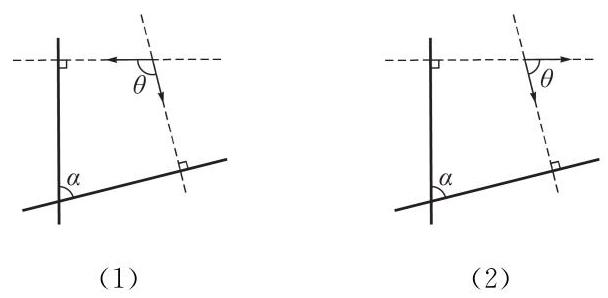
\includegraphics[max width=0.5\textwidth]{images/bo_d7fqvdc91nqc7381i9u0_27_323_1107_608_298_0.jpg}
\end{center}
\hspace*{3em} 

图 1-3-2

把这个一般的讨论用于直线 \({l}_{1}\) 与 \({l}_{2}\) 的情况,则 \({l}_{1} : {a}_{1}x + \; {b}_{1}y + {c}_{1} = 0\) 与 \({l}_{2} : {a}_{2}x + {b}_{2}y + {c}_{2} = 0\) 的夹角 \(\alpha\) 的余弦公式为

\[
\cos \alpha  = \frac{\left| {a}_{1}{a}_{2} + {b}_{1}{b}_{2}\right| }{\sqrt{{a}_{1}^{2} + {b}_{1}^{2}}\sqrt{{a}_{2}^{2} + {b}_{2}^{2}}}.
\]

例 6 求直线 \({l}_{1} : x + {3y} - 1 = 0\) 与 \({l}_{2} : y = {2x} + 7\) 的夹角的大小.

解 直线 \({l}_{2}\) 的一般式方程可写成 \({2x} - y + 7 = 0\) ,因此直线 \({l}_{1}\) 与直线 \({l}_{2}\) 的夹角 \(\alpha\) 的余弦值为

\[
\cos \alpha  = \frac{\left| 2 - 3\right| }{\sqrt{1 + 9} \times  \sqrt{4 + 1}} = \frac{\sqrt{2}}{10},
\]

于是 \(\alpha  = \arccos \frac{\sqrt{2}}{10}\) .

例 7 已知直线 \({l}^{\prime }\) 经过点 \(P\left( {2,1}\right)\) ，与直线 \(l : x + {2y} + 1 = 0\) 夹角为 \(\arccos \frac{\sqrt{5}}{5}\) . 求直线 \({l}^{\prime }\) 的方程.

解 设直线 \({l}^{\prime }\) 的一个法向量为 \(\left( {a,b}\right)\) ,其中 \(a\text{ 、 }b\) 不同时为零,则 \({l}^{\prime }\) 的点法式方程为 \(a\left( {x - 2}\right)  + b\left( {y - 1}\right)  = 0\) .

根据夹角的余弦公式, 得

\[
\frac{\left| a + 2b\right| }{\sqrt{{a}^{2} + {b}^{2}} \cdot  \sqrt{{1}^{2} + {2}^{2}}} = \frac{\sqrt{5}}{5},
\]

化简为 \(3{b}^{2} + {4ab} = 0\) . 所以 \(b = 0\) 或 \(b =  - \frac{4}{3}a\) ,此时 \(a \neq  0\) .

把 \(b = 0\) 或 \(b =  - \frac{4}{3}a\) 代入直线 \({l}^{\prime }\) 的方程，得 \(x = 2\) 或 \(3(x -\) 2) \(- 4\left( {y - 1}\right)  = 0\) .

所以直线 \({l}^{\prime }\) 的方程有两个,一个是 \(x = 2\) ,另一个是 \({3x} - \; {4y} - 2 = 0\) .

\section*{练习 1.3(3)}

1. 根据下列方程,求直线 \({l}_{1}\) 与 \({l}_{2}\) 的夹角的大小:

(1) \({l}_{1} : {3x} - {5y} + 1 = 0\) 与 \({l}_{2} : {2x} + y = 3\) ；

(2) \({l}_{1} : {y = {5x} - 3}\) 与 \({l}_{2} : {y =  - {3x} + 2}\) .

2. 已知直线 \({l}_{1} : \sqrt{3}x - y + 3 = 0\) 与直线 \({l}_{2} : y = {kx} + 3\) 的夹角为 \(\frac{\pi }{4}\) ，求实数 \(k\) 的值.

3. 求经过点 \(A\left( {4, - 3}\right)\) 且与直线 \(l : x + y - 3 = 0\) 的夹角为 \(\frac{\pi }{3}\) 的直线 \({l}^{\prime }\) 的方程.

\section*{习题 1.3}

\section*{A 组}

1. 根据下列方程,判定直线 \({l}_{1}\) 与 \({l}_{2}\) 的位置关系:

(1) \({l}_{1} : {2x} - {3y} - 1 = 0,{l}_{2} : {4x} - {6y} - 2 = 0\) ；

(2) \({l}_{1} : y = \frac{1}{3}x + 1,{l}_{2} : x - {6y} - 2 = 0\) ；

(3) \({l}_{1} : \left( {\sqrt{5} - 1}\right) x - {2y} + 1 = 0,{l}_{2} : {2x} - \left( {\sqrt{5} + 1}\right) y - 2 = 0.\)

2. 已知直线 \({l}_{1} : {6x} + \left( {t - 1}\right) y - 8 = 0\) ，直线 \({l}_{2} : \left( {t + 4}\right) x + \left( {t + 6}\right) y - {16} = 0\) . 根据下列条件,求实数 \(t\) 的取值范围:

(1) \({l}_{1}\) 与 \({l}_{2}\) 相交;

(2) \({l}_{1}//{l}_{2}\) ；

(3) \({l}_{1}\) 与 \({l}_{2}\) 重合.

3. 已知两条直线 \({l}_{1} : \left( {t - 1}\right) x + {2y} - t = 0\) 和 \({l}_{2} : x + {ty} + t - 2 = 0\) ,且 \({l}_{1}//{l}_{2}\) . 求实数 \(t\) 的值.

4. 已知平行四边形 \({ABCD}\) 中,一组对边 \({AB}\text{ 、 }{CD}\) 所在直线的方程分别为 \({ax} + {4y} = a + 2\) , \(x + {ay} = a\) . 求实数 \(a\) 的值.

5. 已知四边形 \({ABCD}\) 的四个顶点的坐标分别为 \(A\left( {-1,2}\right) \text{ 、 }B\left( {3,4}\right) \text{ 、 }C\left( {3,2}\right) \text{ 、 }D\left( {1,1}\right)\) , 求证: 四边形 \({ABCD}\) 是梯形.

6. 已知直线 \({l}_{1} : \left( {k - 3}\right) x + \left( {5 - k}\right) y + 1 = 0\) 与直线 \({l}_{2} : 2\left( {k - 3}\right) x - {2y} + \left( {2 - k}\right)  = 0\) 互相垂直,求实数 \(k\) 的值.

7. 已知直线 \(l\) 垂直于直线 \({l}^{\prime } : {2x} + {3y} - 4 = 0\) ，根据下列条件求 \(l\) 的方程:

(1) \(l\) 经过点 \(\left( {1,1}\right)\) ；

(2) \(l\) 与坐标轴围成的三角形的面积是 3 .

8. 已知等腰直角三角形 \({ABC}\) 的斜边 \({AB}\) 所在直线的方程为 \({3x} - y - 5 = 0\) ,直角顶点为 \(C\left( {4, - 1}\right)\) . 求两条直角边所在直线的方程.

9. 根据下列方程,求直线 \({l}_{1}\) 与 \({l}_{2}\) 的夹角的大小:

(1) \({l}_{1} : {x + {3y} + 2} = 0,{l}_{2} : {{4x} + {2y} - 1} = 0\) ；

(2) \({l}_{1} : {x + {2y} - 3} = 0,{l}_{2} : {x - y - 5} = 0\) ；

(3) \({l}_{1} : {2x} - {3y} + 6 = 0,{l}_{2} : x - 5 = 0\) .

10. 若直线 \(x + {my} + 5 = 0\) 与直线 \(x + y + 1 = 0\) 的夹角为 \(\frac{\pi }{4}\) ,求实数 \(m\) 的值.

11. 已知等腰直角三角形 \({ABC}\) 的直角边 \({BC}\) 所在直线的方程为 \(x - {2y} - 6 = 0\) ,顶点 \(A\) 的坐标为 \(\left( {0,6}\right)\) . 分别求直角边 \({AC}\) 、斜边 \({AB}\) 所在直线的方程.

\section*{B 组}

1. 给定直线 \({l}_{1} : y = {ax} + b\) ,直线 \({l}_{2} : y = {bx} - a\) . 已知直线 \({l}_{1}\) 的倾斜角为 \(\frac{3\pi }{4}\) ,且它与直线 \({l}_{2}\) 的交点落在直线 \({l}_{3} : {2x} + y - 2 = 0\) 上. 求实数 \(b\) 的值.

2. 求证: 不论实数 \(\lambda\) 取何值,直线 \(l : {2x} + y - 4 + \lambda \left( {x - y + 2}\right)  = 0\) 经过同一个点, 并求所有这些直线的公共点.

3. 已知集合 \(A = \{ \left( {x,y}\right)  \mid  {{2x} - \left( {a + 1}\right) y - 1 = 0}\} ,B = \{ \left( {x,y}\right)  \mid  {{ax} - y + 1 = 0}\}\) ,且 \(A \cap  B = \varnothing\) . 求实数 \(a\) 的值.

4. 分别求经过直线 \({l}_{1} : {5x} + {2y} - 3 = 0\) 和 \({l}_{2} : {3x} - {5y} - 8 = 0\) 的交点，且与直线 \(x + {4y} - 7 = 0\) 垂直、平行的直线的方程.

5. 已知 \(\bigtriangleup {ABC}\) 的一个顶点为 \(A\left( {3, - 4}\right)\) ,有两条高所在直线的方程分别是 \({7x} - \; {2y} - 1 = 0\) 与 \({2x} - {7y} - 6 = 0\) . 求 \(\bigtriangleup {ABC}\) 三条边所在直线的方程.

6. 求直线 \({l}_{1} : x + y - 3 = 0\) 与直线 \({l}_{2} : {7x} - y - 5 = 0\) 夹角平分线的方程.

7. 一束光线经过点 \(\left( {-2,1}\right)\) ,由直线 \(l : y = x\) 反射后,经过点 \(\left( {3,5}\right)\) 射出. 求反射光线所在直线的方程.

\section*{1.4 点到直线的距离}

我们首先讨论直线 \(l : {ax} + {by} + c = 0\) ( \(a\text{ 、 }b\) 不同时为零) 外一点 \(P\left( {{x}_{0},{y}_{0}}\right)\) 到这条直线的距离. 根据点到直线距离的定义, 如图 1-4-1,过点 \(P\) 作直线 \(l\) 的垂线,设垂足是 \(Q\left( {{x}_{Q},{y}_{Q}}\right)\) ,则线段 \({PQ}\) 的长度就是点 \(P\) 到直线 \(l\) 的距离 \(d\) . 因此,只要求出 \({PQ}\) 所在直线的方程,然后与 \(l\) 的方程联立得到一个二元一次方程组,解这个方程组就可以得到点 \(Q\) 的坐标,进而利用两点间的距离公式求出 \({PQ}\) 的长度. 这种方法的思路很清晰,但运算量比较大. 为了简便计算, 我们介绍另外一种方法.

\begin{center}
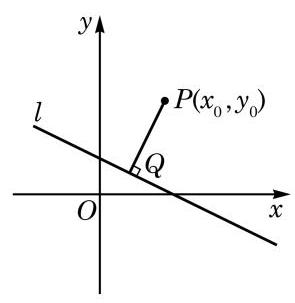
\includegraphics[max width=0.2\textwidth]{images/bo_d7fqvdc91nqc7381i9u0_31_1152_516_295_303_0.jpg}
\end{center}
\hspace*{3em} 

图 1-4-1

由直线 \(l\) 的一般式方程知, \(\overrightarrow{n} = \left( {a,b}\right)\) 是 \(l\) 的一个法向量, 所以 \(\overrightarrow{PQ}//\overrightarrow{n}\) ,即 \(\left| {\cos \langle \overrightarrow{PQ},\overrightarrow{n}\rangle }\right|  = 1\) ,从而

\[
d = \left| \overrightarrow{PQ}\right|  = \frac{\left| \overrightarrow{PQ} \cdot  \overrightarrow{n}\right| }{\left| \overrightarrow{n}\right| } = \frac{\left| a\left( {x}_{Q} - {x}_{0}\right)  + b\left( {y}_{Q} - {y}_{0}\right) \right| }{\sqrt{{a}^{2} + {b}^{2}}}
\]

\[
= \frac{\left| \left( a{x}_{Q} + b{y}_{Q}\right)  - \left( a{x}_{0} + b{y}_{0}\right) \right| }{\sqrt{{a}^{2} + {b}^{2}}}.
\]

因为点 \(Q\) 在 \(l\) 上,所以 \(a{x}_{Q} + b{y}_{Q} + c = 0\) ,即

\[
a{x}_{Q} + b{y}_{Q} =  - c.
\]

所以, \(d = \frac{\left| -c - \left( a{x}_{0} + b{y}_{0}\right) \right| }{\sqrt{{a}^{2} + {b}^{2}}}\) ,从而得到点 \(P\left( {{x}_{0},{y}_{0}}\right)\) 到直线 \(l : {ax} + {by} + c = 0\) 的距离公式

\[
d = \frac{\left| a{x}_{0} + b{y}_{0} + c\right| }{\sqrt{{a}^{2} + {b}^{2}}}.
\]

当点 \(P\) 在直线 \(l\) 上时,上述公式仍然成立,此时 \(d = 0\) .

例 1 根据下列条件,求点 \(P\) 到直线 \(l\) 的距离 \(d\) :

(1) \(P\left( {1,2}\right) ,l : x + {2y} + 5 = 0\) ;

(2) \(P\left( {-\sqrt{3},3}\right) ,l : y = \sqrt{3}x + 3\) .

解(1)由点到直线的距离公式, 得

\[
d = \frac{\left| 1 + 2 \times  2 + 5\right| }{\sqrt{{1}^{2} + {2}^{2}}} = 2\sqrt{5}.
\]

(2)将直线 \(l\) 的方程化为 \(\sqrt{3}x - y + 3 = 0\) ，所以由点到直线的距离公式, 得

\[
d = \frac{\left| \sqrt{3} \times  \left( -\sqrt{3}\right)  + \left( -1\right)  \times  3 + 3\right| }{\sqrt{{\left( \sqrt{3}\right) }^{2} + {\left( -1\right) }^{2}}} = \frac{3}{2}.
\]

例 2 求平行直线 \({l}_{1} : \sqrt{2}x + y + 1 = 0\) 与 \({l}_{2} : \sqrt{2}x + y + 4 = 0\) 之间的距离.

解 两条平行线之间的距离就是其中一条直线上的一点到另一条直线的距离. 为方便计算,我们在直线 \({l}_{1}\) 上取一个特殊点 \(P\left( {0, - 1}\right)\) ,点 \(P\) 到直线 \({l}_{2} : \sqrt{2}x + y + 4 = 0\) 的距离为

\[
d = \frac{\left| \sqrt{2} \times  0 + 1 \times  \left( -1\right)  + 4\right| }{\sqrt{2 + 1}} = \sqrt{3}.
\]

所以,直线 \({l}_{1}\) 与 \({l}_{2}\) 之间的距离为 \(\sqrt{3}\) .

如图 1-4-2,对于两条平行线 \({l}_{1} : {ax} + {by} + {c}_{1} = 0\) 与 \({l}_{2} : {ax} + \; {by} + {c}_{2} = 0\left( {a\text{ 、 }b}\right.\) 不同时为零),我们可以采取同样的方法求它们之间的距离. 取 \({l}_{1}\) 上一点 \(P\left( {{x}_{0},{y}_{0}}\right)\) ,则 \(a{x}_{0} + b{y}_{0} + {c}_{1} = 0\) . 点 \(P\) 到 \({l}_{2}\) 的距离 \(d = \frac{\left| a{x}_{0} + b{y}_{0} + {c}_{2}\right| }{\sqrt{{a}^{2} + {b}^{2}}}\) . 由 \(a{x}_{0} + b{y}_{0} + {c}_{1} = 0\) ,得 \(a{x}_{0} + \; b{y}_{0} =  - {c}_{1}\) ,所以 \(d = \frac{\left| -{c}_{1} + {c}_{2}\right| }{\sqrt{{a}^{2} + {b}^{2}}}\) . 也就是说: 平行线 \({l}_{1} : {ax} + \; {by} + {c}_{1} = 0\) 与 \({l}_{2} : {ax} + {by} + {c}_{2} = 0\) 的距离为

\[
d = \frac{\left| {c}_{1} - {c}_{2}\right| }{\sqrt{{a}^{2} + {b}^{2}}}.
\]

\begin{center}
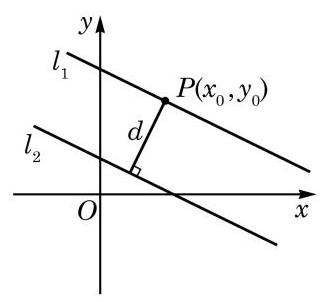
\includegraphics[max width=0.2\textwidth]{images/bo_d7fqvdc91nqc7381i9u0_32_185_1013_323_302_0.jpg}
\end{center}
\hspace*{3em} 

图 1-4-2

例 3 已知直线 \({l}_{1} : y = \sqrt{2}x + 1\) ，直线 \({l}_{2}\) 与 \({l}_{1}\) 平行，且与 \({l}_{1}\) 的距离为 2 . 求直线 \({l}_{2}\) 的方程.

解 由题意,可设 \({l}_{2}\) 的方程为 \(y = \sqrt{2}x + b\left( {b \in  \mathbf{R}\text{ 且 }b \neq  1}\right)\) .

直线 \({l}_{1}\) 与 \({l}_{2}\) 的一般式方程为

\[
{l}_{1} : \sqrt{2}x - y + 1 = 0\text{ 与 }{l}_{2} : \sqrt{2}x - y + b = 0.
\]

由两条平行直线之间的距离公式, 得

\[
\frac{\left| 1 - b\right| }{\sqrt{{1}^{2} + {\left( \sqrt{2}\right) }^{2}}} = 2.
\]

解得 \(b = 2\sqrt{3} + 1\) 或 \(b =  - 2\sqrt{3} + 1\) .

所以,直线 \({l}_{2}\) 的方程为 \(y = \sqrt{2}x + 2\sqrt{3} + 1\) 或 \(y = \sqrt{2}x - 2\sqrt{3} + 1\) .

\section*{练习 1.4}

1. 根据下列条件,求点 \(M\left( {-2, - 1}\right)\) 到直线 \(l\) 的距离 \(d\) :

(1) \(l : x = 3\)

(2) \(l : y = 3\) ；

(3) \(l : {x + y} = {3;}\)

(4) \(l : y = {3x} - 5\) .

2. 在直角三角形 \({ABC}\) 中, \(\angle A = \frac{\pi }{2},\left| {AB}\right|  = 6,\left| {AC}\right|  = 8\) . 求三角形的重心 \(G\) 到斜边 \({BC}\) 所在直线的距离.

\section*{习题 1.4}

\section*{A 组}

1. 求点 \(P\left( {2,3}\right)\) 到直线 \(l\) 的距离:

(1) \(l : {3x} - {2y} = {13}\) ；

(2) \(l : y =  - {2x} + 3\) .

2. 已知点 \(A\left( {a,6}\right)\) 到直线 \({3x} - {4y} - 4 = 0\) 的距离等于 4,求实数 \(a\) 的值.

3. 求下列两条平行线之间的距离:

(1) \({l}_{1} : {2x} - {3y} + 1 = 0,{l}_{2} : {4x} - {6y} + 1 = 0\) ；

(2) \({l}_{1} : y = \frac{\sqrt{3}}{2}x + 1,{l}_{2} : \sqrt{3}x - {2y} + 1 = 0\) .

4. 已知直线 \({l}_{1} : {2x} - y + a = 0\) 与直线 \({l}_{2} :  - {4x} + {2y} + 1 = 0\) 的距离为 \(\frac{7\sqrt{5}}{10}\) ，求实数 \(a\) 的值.

B 组

1. 已知点 \(A\left( {1,0}\right) \text{ 、 }B\left( {4, - 4}\right)\) . 若点 \(A\) 与点 \(B\) 到直线 \(l\) 的距离都为 2,求直线 \(l\) 的方程.

2. 已知点 \(P\) 是直线 \({3x} - {4y} + 2 = 0\) 上任意一点,求点 \(P\) 与点 \(A\left( {3, - 1}\right)\) 之间距离的最小值.

3. 已知直线 \(l\) 经过点 \(P\left( {1,1}\right)\) 且与直线 \({l}_{1} : y = \sqrt{3}x + 1\) 和 \({l}_{2} : y = \sqrt{3}x + 3\) 分别交于点 \(A\) 和点 \(B\) . 若 \(\left| {AB}\right|  = \sqrt{2}\) ,求直线 \(l\) 的方程.

\section*{课后阅读}

\section*{解析几何的诞生}

文艺复兴以来，生产力的发展对科学技术提出了全新的要求. 到 16 世纪，对运动与变化的研究已成为自然科学的中心问题. 这迫切需要一种新的数学工具, 从而诞生了解析几何.

有别于传统的纯几何方法, 解析几何将数与形有机地结合起来, 形成一门新的学科. 它的基本思想是在平面上引进 “坐标” 的概念, 并借助于平面上的点和有序实数对之间所建立的一一对应关系, 将一个代数方程与平面上一条曲线对应起来. 于是几何问题便可归结为代数问题, 反过来又可通过代数问题的研究发现新的几何结果.

借助于坐标来确定点的位置的思想在古代曾经出现过, 古希腊数学家阿波罗尼斯 (Apollonius)关于圆锥曲线性质的推导, 阿拉伯数学家通过圆锥曲线交点求解三次方程的研究, 都蕴含着这种思想.

解析几何的建立主要归功于两位 17 世纪的法国数学家笛卡儿 (R. Descartes) 和费马 (P. de Fermat). 他们工作的出发点不同, 却殊途同归.

1637 年笛卡儿出版了著名的哲学著作《方法论》，该书有三个附录，《几何学》是其中之一, 解析几何的发明就在这篇附录中. 笛卡儿的出发点是一个著名的古希腊数学问题: 帕普斯问题. 笛卡儿解决了一些特殊的情形, 由此建立起了历史上第一个斜坐标系. 在 《几何学》中, 笛卡儿也给出了直角坐标系的例子. 基于坐标系和曲线方程的思想, 笛卡儿还提出了一系列新颖的想法. 例如, 曲线的次数与坐标轴的选择无关, 利用曲线的方程表示求出两条不同曲线的公共点, 曲线的分类, 等等.

与笛卡儿不同, 费马工作的出发点是想恢复已失传的阿波罗尼斯的《论平面轨迹》, 为此, 他写成《平面与立体轨迹引论》(1629)一书，其中清晰地阐述了自己的解析几何思想. 费马在书中写道:“在最后的方程中出现两个未知量时，我们就得到一个轨迹，其中一个未知量的一端画出了一条直线或曲线. ”这就是说，用代数方法解几何问题时，最后得到含两个未知量的方程, 所得结果表示一轨迹 (直线或曲线). 因此, 费马以研究古希腊轨迹问题为目的, 以韦达(F. Viète)的符号代数为工具, 通过建立只含一条轴的坐标系, 将二元代数方程与几何曲线对应起来, 导引着解析几何的诞生.

解析几何的发明具有伟大的意义. 它使得原先以常量为主导的数学转变为以变量为主导的数学, 从而为微积分的创立搭起数学舞台; 它使得代数和几何融合为一体, 实现了几何图形的代数化; 经由代数和几何的相互转化, 它使数学家得以摆脱现实的束缚, 从三维空间进入高维空间, 探索更深层次的概念.

解析几何为我们打开了一扇通往全新数学世界的大门. 在解析几何诞生的背后, 蕴藏诸多有趣的数学故事, 充分体现了数学的人文精神.

\section*{内容提要}

1. 与平面直角坐标中直线有关的重要的量

(1)倾斜角:当直线 \(l\) 与 \(x\) 轴相交于一点 \(A\) 时，将 \(x\) 轴绕点 \(A\) 沿逆时针方向旋转到与 \(l\) 重合时所转过的最小正角 \(\theta\) 称为直线 \(l\) 的倾斜角；当 \(l\) 平行于 \(x\) 轴或与 \(x\) 轴重合时， 规定倾斜角 \(\theta  = 0\) . 于是，倾斜角的取值范围为 \(0 \leq  \theta  < \pi\) .

(2)斜率:当直线 \(l\) 不与 \(x\) 轴垂直时，定义它的斜率为 \(k = \tan \theta\) ，其中 \(\theta\) 为 \(l\) 的倾斜角; 当直线 \(l\) 与 \(x\) 轴垂直时,斜率不存在. 过两点 \(A\left( {{x}_{1},{y}_{1}}\right)\) 与 \(B\left( {{x}_{2},{y}_{2}}\right) \left( {{x}_{1} \neq  {x}_{2}}\right)\) 的直线的斜率是 \(k = \frac{{y}_{2} - {y}_{1}}{{x}_{2} - {x}_{1}}\) .

(3)截距:直线 \(l\) 与 \(y\) 轴交点的纵坐标称为直线 \(l\) 在 \(y\) 轴上的截距；直线 \(l\) 与 \(x\) 轴交点的横坐标称为直线 \(l\) 在 \(x\) 轴上的截距.

2. 直线的各种形式的方程

(1)直线的点斜式方程:过点 \(M\left( {{x}_{0},{y}_{0}}\right)\) 且斜率为 \(k\) 的直线的方程是 \(y - {y}_{0} = k\left( {x - {x}_{0}}\right)\) .

(2)直线的斜截式方程:斜率为 \(k\) 且在 \(y\) 轴上的截距为 \(b\) 的直线的方程是 \(y = {kx} + b\) .

(3)直线的两点式方程:经过两点 \(M\left( {{x}_{1},{y}_{1}}\right)\) 、 \(N\left( {{x}_{2},{y}_{2}}\right)\) ( \({x}_{1} \neq  {x}_{2}\) 且 \({y}_{1} \neq  {y}_{2}\) )的直线的方程是 \(\frac{y - {y}_{1}}{{y}_{2} - {y}_{1}} = \frac{x - {x}_{1}}{{x}_{2} - {x}_{1}}\) .

(4)直线的点法式方程:过点 \(M\left( {{x}_{0},{y}_{0}}\right)\) 且一个法向量为 \(\overrightarrow{n} = \left( {a,b}\right)\) 的直线的方程是 \(a\left( {x - {x}_{0}}\right)  + b\left( {y - {y}_{0}}\right)  = 0.\)

(5)直线的一般式方程:直线一般形式的方程是 \({ax} + {by} + c = 0\) ，其中 \(a\) 、 \(b\) 不同时为零. 这个方程的一次项系数给出了它的一个法向量 \(\overrightarrow{n} = \left( {a,b}\right)\) .

3. 两条直线的位置关系

给定两条直线 \({l}_{1} : {a}_{1}x + {b}_{1}y + {c}_{1} = 0\) 与 \({l}_{2} : {a}_{2}x + {b}_{2}y + {c}_{2} = 0\) ( \({a}_{1}\text{ 、 }{b}_{1}\) 不同时为零, \({a}_{2}\text{ 、 }{b}_{2}\) 不同时为零).

(1)直线相交、平行与重合: \({l}_{1}\) 与 \({l}_{2}\) 相交、平行或重合取决于方程组 \(\left\{  \begin{array}{l} {a}_{1}x + {b}_{1}y + {c}_{1} = 0, \\  {a}_{2}x + {b}_{2}y + {c}_{2} = 0 \end{array}\right.\) 解的情况:

 \circled{1}  \({l}_{1}\) 与 \({l}_{2}\) 重合 \(\Leftrightarrow\) 方程组有无数组解 \(\Leftrightarrow\) 存在 \(\lambda  \in  \mathbf{R}\) ，使得 \({a}_{1} = \lambda {a}_{2},{b}_{1} = \lambda {b}_{2}\) 且 \({c}_{1} = \lambda {c}_{2}\) ；

 \circled{2}  \({l}_{1}//{l}_{2} \Leftrightarrow\) 方程组无解 \(\Leftrightarrow\) 存在 \(\lambda  \in  \mathbf{R}\) ，使得 \({a}_{1} = \lambda {a}_{2}\) ， \({b}_{1} = \lambda {b}_{2}\) 但 \({c}_{1} \neq  \lambda {c}_{2}\) ；

 \circled{3}  \({l}_{1}\) 与 \({l}_{2}\) 相交 \(\Leftrightarrow\) 方程组有唯一的解 \(\Leftrightarrow  {a}_{1}{b}_{2} \neq  {a}_{2}{b}_{1}\) .

(2)两条直线垂直的充要条件: \({l}_{1} \bot  {l}_{2} \Leftrightarrow  {a}_{1}{a}_{2} + {b}_{1}{b}_{2} = 0\) ；如果两条直线的斜率 \({k}_{1}\) 与 \({k}_{2}\) 都存在,那么 \({l}_{1} \bot  {l}_{2} \Leftrightarrow  {k}_{1}{k}_{2} =  - 1\) .

(3)两条直线的夹角: \({l}_{1}\) 与 \({l}_{2}\) 的夹角 \(\alpha\) 的余弦公式为

\[
\cos \alpha  = \frac{\left| {a}_{1}{a}_{2} + {b}_{1}{b}_{2}\right| }{\sqrt{{a}_{1}^{2} + {b}_{1}^{2}}\sqrt{{a}_{2}^{2} + {b}_{2}^{2}}}.
\]

4. 点到直线的距离:点 \(P\left( {{x}_{0},{y}_{0}}\right)\) 到直线 \({ax} + {by} + c = 0\left( {a\text{ 、 }b}\right.\) 不同时为零)的距离为 \(d = \frac{\left| a{x}_{0} + b{y}_{0} + c\right| }{\sqrt{{a}^{2} + {b}^{2}}}.\)

\section*{复习题}

\section*{A 组}

1. 求直线 \(\sqrt{2}x - {4y} + 5 = 0\) 的倾斜角. (用 arctan 表示)

2. 若直线 \({ax} + {2y} + 6 = 0\) 和直线 \(x + a\left( {a + 1}\right) y + \left( {{a}^{2} - 1}\right)  = 0\) 互相垂直，求实数 \(a\) 的值.

3. 直线 \(x - y + 1 = 0\) 上一点 \(P\) 的横坐标是 3,若该直线绕点 \(P\) 逆时针旋转 \({90}^{ \circ  }\) 得到直线 \(l\) ,求直线 \(l\) 的方程.

4. 设直线 \(x - {ay} - 4 = 0\) 与直线 \(y =  - {2x} + 4\) 的夹角为 \(\arccos \frac{2\sqrt{5}}{5}\) ,求实数 \(a\) 的值.

5. 已知 \(\alpha  \in  \left\lbrack  {0,\frac{\pi }{2}}\right)\) ,求直线 \(x\cos \alpha  + \sqrt{3}y + 2 = 0\) 的倾斜角的取值范围.

6. 求过点 \(\left( {3, - 2}\right)\) 且在 \(x\) 轴、 \(y\) 轴上截距相等的直线的方程.

7. 已知点 \(P\left( {1,1}\right)\) 到直线 \(x + {ay} - 2 = 0\) 的距离为 1,求实数 \(a\) 的值.

8. 已知平行四边形 \({ABCD}\) 中,边 \({AB}\) 所在直线的方程为 \(x + y - 1 = 0\) ,边 \({AD}\) 所在直线的方程为 \({3x} - y + 4 = 0\) .

(1)求点 \(A\) 的坐标；

(2)若点 \(C\) 的坐标为 \(\left( {3,3}\right)\) ，分别求边 \({BC}\) 与 \({DC}\) 所在直线的方程.

9. 已知直线 \({l}_{1} : x + {my} + 6 = 0,{l}_{2} : \left( {m - 2}\right) x + {3y} + {2m} = 0\) ,求实数 \(m\) 的取值范围, 使得:

(1) \({l}_{1}\) 与 \({l}_{2}\) 相交; (2) \({l}_{1} \bot  {l}_{2}\) ；

(3) \({l}_{1}//{l}_{2}\) ； (4) \({l}_{1}\) 与 \({l}_{2}\) 重合.

10. 已知直线 \(l\) 与两坐标轴围成一个等腰直角三角形,且此三角形的面积为 \(\frac{49}{2}\) . 求直线 \(l\) 的方程.

11. 在 \(\bigtriangleup {ABC}\) 中,边 \({AB}\text{ 、 }{AC}\) 上的高所在直线的方程分别为 \({2x} - {3y} + 1 = 0\) 与 \(x + y = 0\) , 点 \(A\) 的坐标为 \(\left( {1,2}\right)\) . 求边 \({BC}\) 所在直线的方程.

12. 已知直线 \(l\) 垂直于直线 \({3x} + {4y} - 9 = 0\) ,点 \(A\left( {2,3}\right)\) 到直线 \(l\) 的距离为 1 . 求直线 \(l\) 的方程.

13. 已知三条直线 \({l}_{1} : {ax} + {by} + 4 = 0,{l}_{2} : \left( {a - 1}\right) x + y + b = 0,{l}_{3} : x + {2y} + 3 = 0\) .

(1)若 \({l}_{1} \bot  {l}_{2}\) 且 \({l}_{1}\) 经过点 \(\left( {-1,1}\right)\) ，求 \(a\) 、 \(b\) 的值；

(2)若 \({l}_{1}//{l}_{2}//{l}_{3}\) ，求 \(a\) 、 \(b\) 的值.

\section*{B 组}

1. 已知过点 \(\left( {0, - 2}\right)\) 且具有斜率 \(k\) 的直线 \(l\) 与以点 \(A\left( {3,1}\right)\) 和 \(B\left( {-2,5}\right)\) 为端点的线段 \({AB}\) 相交,求实数 \(k\) 的取值范围.

2. 已知两条直线 \({l}_{1} : y - x = 0,{l}_{2} : y = {ax}\) ，其中 \(a \in  \mathbf{R}\) . 当这两条直线的夹角在 \(\left( {0,\frac{\pi }{12}}\right)\) 内变化时,求实数 \(a\) 的取值范围.

3. 直线 \(l\) 过原点且平分平行四边形 \({ABCD}\) 的面积,若此平行四边形的两个顶点为 \(B\left( {1,4}\right) \text{ 、 }D\left( {5,0}\right)\) ,求直线 \(l\) 的方程.

4. 求直线 \({l}_{1} : {3x} - {2y} - 6 = 0\) 关于直线 \({l}_{2} : {2x} - {3y} + 1 = 0\) 对称的直线 \({l}_{3}\) 的方程.

5. 已知动点 \(M\left( {a,b}\right)\) 在直线 \({3x} + {4y} - {15} = 0\) 上,求 \(\sqrt{{a}^{2} + {b}^{2}}\) 的最小值.

6. 已知两条平行直线 \({l}_{1}\) 与 \({l}_{2}\) 分别过点 \({P}_{1}\left( {1,0}\right)\) 与点 \({P}_{2}\left( {0,5}\right) ,{l}_{1}\text{ 、 }{l}_{2}\) 之间的距离为 \(d\) . 求 \(d\) 的最大值,并指出此时 \({l}_{1}\text{ 、 }{l}_{2}\) 的方程.

7. 已知直线 \(l\) 经过点 \(C\left( {2,1}\right)\) ，且与 \(x\) 轴、 \(y\) 轴的正半轴分别交于点 \(A\) 、点 \(B,O\) 是坐标原点.

(1)当 \(\bigtriangleup  {AOB}\) 的面积最小时，求直线 \(l\) 的方程；

(2)当 \(\left| {CA}\right|  \cdot  \left| {CB}\right|\) 取最小值时，求直线 \(l\) 的方程，并求此最小值.

\section*{拓展与思考}

1. 作出方程 \(\left| x\right|  + \left| y\right|  = 1\) 所表示的图形,并求该图形围成的区域的面积.

2. 给定直线 \({l}_{1} : y = {k}_{1}x + {b}_{1}\) 与 \({l}_{2} : y = {k}_{2}x + {b}_{2}\) ,求证: 如果直线 \({l}_{1}\) 与 \({l}_{2}\) 不互相垂直,那么它们的夹角 \(\alpha\) 满足 \(\tan \alpha  = \left| \frac{{k}_{1} - {k}_{2}}{1 + {k}_{1}{k}_{2}}\right|\) .

3. 已知直线 \({l}_{1} : {4x} + y = 4,{l}_{2} : {mx} + y = 0,{l}_{3} : {2x} - {3my} = 4\) . 当 \(m\) 为何值时,它们不能围成三角形?

4. 点到直线的距离是该点到直线上任意一点距离的最小值. 如果把一个给定点到线段上任意一点的距离的最小值定义为该点到该线段的距离,试求点 \(P\left( {1,1}\right)\) 到线段 \(l : x - \; y - 3 = 0\left( {3 \leq  x \leq  5}\right)\) 的距离.

\begin{center}
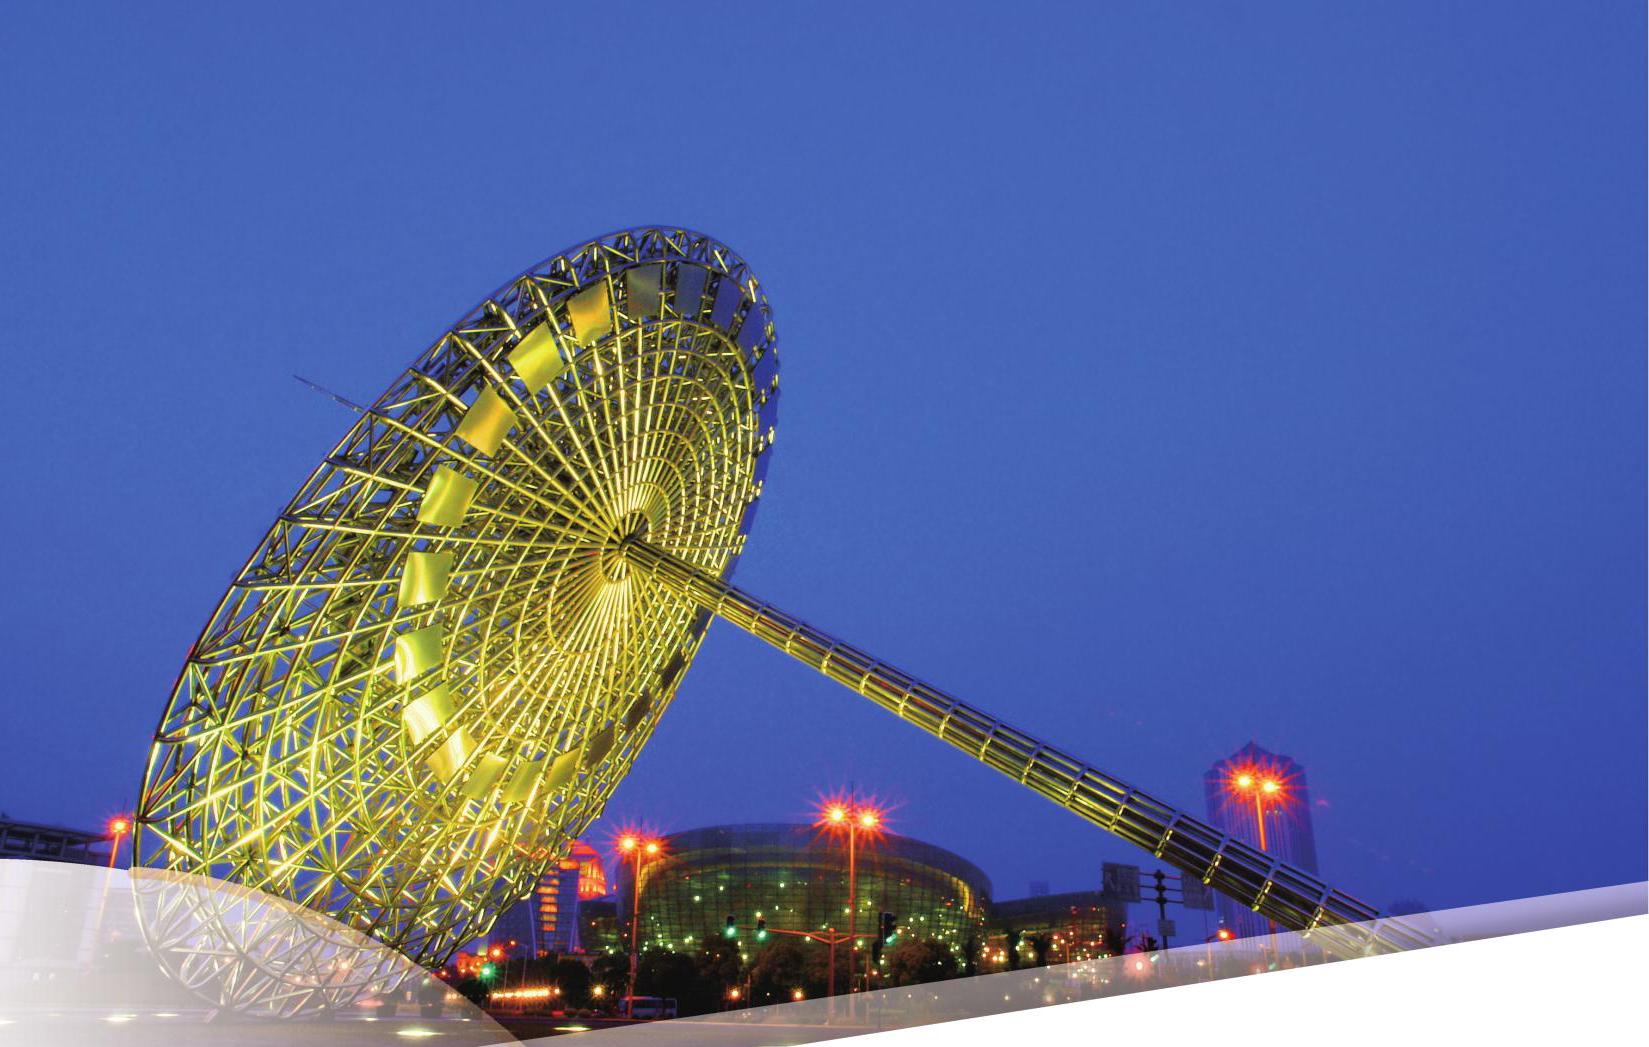
\includegraphics[max width=1.0\textwidth]{images/bo_d7fqvdc91nqc7381i9u0_39_5_0_1649_1047_0.jpg}
\end{center}
\hspace*{3em} 

\section*{第 2 章 圆锥曲线}

在上一章中, 我们初步领略了解析几何的一些基本特点, 知道通过建立平面直角坐标系得到直线的方程, 然后利用方程讨论点与直线、直线与直线的位置关系. 在这一章中, 通过对圆锥曲线的研究, 我们进一步深入解析几何的核心领域并体验解析几何的思想和作用.

对圆锥曲线的研究虽然可以追溯到两千多年前的古希腊时代，但直到笛卡儿坐标系的引入，才找到更一般且统一的处理方法. 在直角坐标平面上, 所有圆锥曲线都可以用二元二次方程来表示, 从而可以用方程的思想去解决与这些曲线有关的问题. 由于圆锥曲线是日常生活中常见的曲线, 在航天、航海、光学等领域都有广泛的应用, 这使得解析几何成为数学的一个重要分支.

除了直线和圆以外, 椭圆、双曲线和抛物线已经与平面几何所涉及的内容有本质的区别, 但却与函数有了联系, 如反比例函数的图像是双曲线、二次函数的图像是抛物线等.

\section*{2.1 圆}

\section*{1 曲线方程的概念}

在上一章 1.2 节中, 我们针对具体的例子解释了什么是 “直线的方程”, 从而引导了全章的学习. 通过上一章的学习, 我们对“直线方程”有了更多认识. 在此基础上我们不难总结出 “直线方程” 的严格定义: 在一个平面直角坐标系中给定一条直线和一个关于 \(x\) 与 \(y\) 的二元一次方程,如果给定直线上的每一个点的坐标都是该给定方程的解, 而且以给定方程的解为坐标的点都在该给定直线上, 那么称这个给定的方程是给定直线的方程.

如果考虑更为一般的平面曲线 (直线是它的特例), 可以直接把这个定义推广而给出曲线方程的概念: 在一个平面直角坐标系中给定一条曲线和一个关于 \(x\) 与 \(y\) 的二元方程,如果给定曲线上的每一个点的坐标都是该给定方程的解, 而且以给定方程的解为坐标的点都在该给定曲线上, 那么称这个给定的方程是给定曲线的方程, 也称这条给定的曲线是给定方程的曲线.

\section*{2 圆的标准方程}

在各种非直线的平面曲线中, 我们最熟悉的是圆.

在平面几何中已经知道, 圆 (circle) 是到一个定点的距离等于定长 (大于零) 的点的轨迹. 这个定点就是圆心 (center), 定长就是圆的半径 (radius). 如果一个圆在直角坐标平面上, 我们该如何确定这个圆的位置, 并且建立圆的方程呢?

显然, 只要圆心的位置及圆的半径确定, 一个圆在平面上的位置就完全确定了. 假设在平面直角坐标系中,已知圆 \(C\) 的圆心是 \(C\left( {a,b}\right)\) ,半径是 \(r\left( {r > 0}\right)\) ,如图 2-1-1 所示. 我们来考察这个圆上的动点 \(P\left( {x,y}\right)\) 的坐标所满足的方程.

\begin{center}
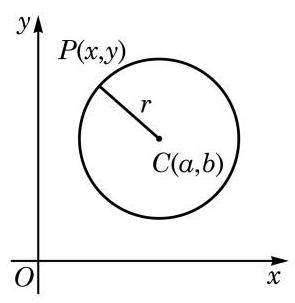
\includegraphics[max width=0.2\textwidth]{images/bo_d7fqvdc91nqc7381i9u0_41_1154_236_295_303_0.jpg}
\end{center}
\hspace*{3em} 

图 2-1-1

因为 \(\left| {PC}\right|  = r\) ,即 \(\sqrt{{\left( x - a\right) }^{2} + {\left( y - b\right) }^{2}} = r\) ,两边平方后得

\[
{\left( x - a\right) }^{2} + {\left( y - b\right) }^{2} = {r}^{2},
\]
  \circled{1} 

所以圆 \(C\) 上任意一点 \(P\left( {x,y}\right)\) 的坐标都满足方程 \circled{1} .

反之,若平面上有一点 \(M\) 的坐标 \(\left( {{x}_{1},{y}_{1}}\right)\) 是方程 \circled{1} 的解,则 \({\left( {x}_{1} - a\right) }^{2} + {\left( {y}_{1} - b\right) }^{2} = {r}^{2}\) ,即 \({\left| MC\right| }^{2} = {r}^{2}\) ,可得 \(\left| {MC}\right|  = r\) . 所以,点 \(M\) 在以 \(C\) 为圆心、以 \(r\) 为半径的圆上.

因此,方程 \circled{1} 是圆 \(C\) 的方程. 我们把它叫做圆的标准方程.

特别地,当 \(a = b = 0\) ,即圆心在原点 \(O\left( {0,0}\right)\) 时,圆的标准方程为

\[
{x}^{2} + {y}^{2} = {r}^{2}.
\]

\HRule

若设 \(N\left( {x,y}\right)\) 为圆 \(C\) 上任意一点,能否由 \(\overrightarrow{NP} \bot  \overrightarrow{NQ}\) 求得圆 \(C\) 的方程?

\HRule

例 1 已知两点 \(P\left( {3,4}\right) \text{ 、 }Q\left( {-5,6}\right)\) ,求以 \({PQ}\) 为直径的圆 \(C\) 的方程.

解 由已知,圆心 \(C\) 为线段 \({PQ}\) 的中点,可得圆心 \(C\) 的坐标为 \(\left( {-1,5}\right)\) .

又半径 \(r\) 为直径 \({PQ}\) 长度的一半,即

\[
r = \frac{1}{2}\left| {PQ}\right|  = \frac{1}{2}\sqrt{{\left( -5 - 3\right) }^{2} + {\left( 6 - 4\right) }^{2}} = \sqrt{17}.
\]

因此,所求圆的标准方程为 \({\left( x + 1\right) }^{2} + {\left( y - 5\right) }^{2} = {17}\) .

例 2 设平面上有一条长度为 4 的线段 \({AB}\) ,试建立适当的平面直角坐标系,求到线段 \({AB}\) 两端点的距离的平方和为 16 的点的轨迹方程.

\begin{center}
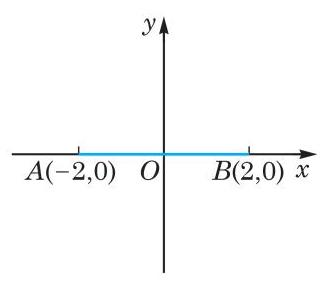
\includegraphics[max width=0.2\textwidth]{images/bo_d7fqvdc91nqc7381i9u0_41_1139_1723_322_281_0.jpg}
\end{center}
\hspace*{3em} 

图 2-1-2

解 如图 2-1-2,取 \({AB}\) 的中点 \(O\) 为原点, \({AB}\) 所在直线为 \(x\) 轴,射线 \({OB}\) 方向为它的正方向,以过点 \(O\) 且垂直于 \({AB}\) 的直线为 \(y\) 轴,建立平面直角坐标系,则有 \(A\left( {-2,0}\right) \text{ 、 }B\left( {2,0}\right)\) .

设点 \(P\left( {x,y}\right)\) 到 \(A\text{ 、 }B\) 两点的距离的平方和为 16,就有

\[
\left\lbrack  {{\left( x + 2\right) }^{2} + {y}^{2}}\right\rbrack   + \left\lbrack  {{\left( x - 2\right) }^{2} + {y}^{2}}\right\rbrack   = {16},
\]

化简, 得

\[
{x}^{2} + {y}^{2} = 4
\]

因此,所求轨迹方程为 \({x}^{2} + {y}^{2} = 4\) ,其轨迹是以 \(O\left( {0,0}\right)\) 为圆心、以 \({AB}\) 为直径的圆.

\begin{center}
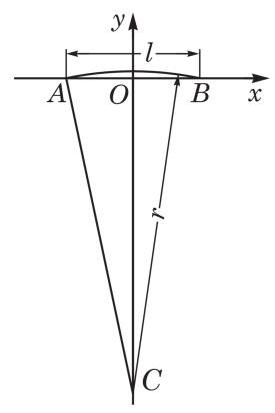
\includegraphics[max width=0.2\textwidth]{images/bo_d7fqvdc91nqc7381i9u0_42_208_351_275_413_0.jpg}
\end{center}
\hspace*{3em} 

图 2-1-3

例 3 造船时, 为了船体放样, 要画出甲板圆弧线. 由于这条圆弧线的半径很大, 无法直接在钢板上用圆规画出, 需要先建立这条圆弧线的方程, 再用描点法画出圆弧线. 如图 2-1-3, 已知圆弧 \(\overset{\text{ ⏜ }}{AB}\) 的半径 \(r\) 为 \({29}\mathrm{\;m}\) ,圆弧 \(\overset{\text{ ⏜ }}{AB}\) 所对的弦长 \(l\) 为 \({12}\mathrm{\;m}\) , 以 \(\mathrm{m}\) 为单位,建立适当的平面直角坐标系,并求圆弧 \(\overset{\text{ ⏜ }}{AB}\) 的方程. (结果精确到 \({0.001}\mathrm{\;m}\) )

解 以弦 \({AB}\) 所在直线为 \(x\) 轴 (射线 \({AB}\) 方向为 \(x\) 轴正方向), 弦 \({AB}\) 的垂直平分线为 \(y\) 轴,建立平面直角坐标系. 可知弦的端点坐标分别为 \(A\left( {-6,0}\right) \text{ 、 }B\left( {6,0}\right)\) .

设圆弧的圆心为 \(C\) ,连接 \({AC}\) ,则

\[
\left| {AO}\right|  = \frac{1}{2}\left| {AB}\right|  = 6\left( \mathrm{\;m}\right) ,\left| {AC}\right|  = r = {29}\left( \mathrm{\;m}\right) ,
\]

从而

\[
\left| {OC}\right|  = \sqrt{{\left| AC\right| }^{2} - {\left| AO\right| }^{2}} = \sqrt{{29}^{2} - {6}^{2}} \approx  {28.373}\left( \mathrm{\;m}\right) ,
\]

即圆心的坐标为 \(C\left( {0, - {28.373}}\right)\) .

所以,圆弧 \(\overset{\text{ ⏜ }}{AB}\) 的方程为 \({x}^{2} + {\left( y + {28.373}\right) }^{2} = {841}( - 6 \leq  x \leq  6\) , \(y \geq  0)\) .

例 4 已知一个圆与 \(y\) 轴相切,其圆心在直线 \(x - {3y} = 0\) 上,且直线 \(y = x\) 被该圆截得的弦长为 \(2\sqrt{7}\) . 求此圆的方程.

\begin{center}
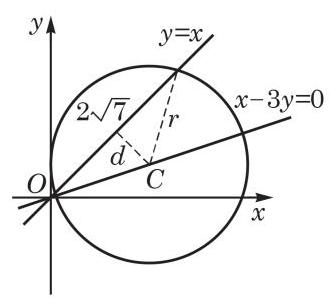
\includegraphics[max width=0.2\textwidth]{images/bo_d7fqvdc91nqc7381i9u0_42_183_1350_331_304_0.jpg}
\end{center}
\hspace*{3em} 

图 2-1-4

解 如图 2-1-4,设所求圆的圆心为 \(C\left( {a,b}\right)\) ,半径为 \(r\) ,则由圆心在直线 \(x - {3y} = 0\) 上,得 \(a = {3b}\) ,又圆与 \(y\) 轴相切,得半径 \(r = \left| a\right|\) .

圆心到直线 \(x - y = 0\) 的距离

\[
d = \frac{\left| a - b\right| }{\sqrt{2}} = \frac{\left| 3b - b\right| }{\sqrt{2}} = \sqrt{2}\left| b\right| ,
\]

由勾股定理,可得 \({r}^{2} - {d}^{2} = {\left( \sqrt{7}\right) }^{2}\) ,即

\[
{\left| a\right| }^{2} - {\left( \sqrt{2}\left| b\right| \right) }^{2} = 9{b}^{2} - 2{b}^{2} = 7{b}^{2} = 7,
\]

解得

\[
b =  \pm  1\text{ . }
\]

当 \(b = 1\) 时, \(a = 3,r = 3\) ,圆的方程为 \({\left( x - 3\right) }^{2} + {\left( y - 1\right) }^{2} = 9\) ;

当 \(b =  - 1\) 时, \(a =  - 3,r = 3\) ,圆的方程为 \({\left( x + 3\right) }^{2} + {\left( y + 1\right) }^{2} = 9\) .

因此,所求圆的方程为 \({\left( x - 3\right) }^{2} + {\left( y - 1\right) }^{2} = 9\) 或 \({\left( x + 3\right) }^{2} + \; {\left( y + 1\right) }^{2} = 9.\)

1. 求以 \(C\left( {3,4}\right)\) 为圆心,且过点 \(M\left( {1, - 3}\right)\) 的圆的方程.

2. 求以 \(C\left( {-1,2}\right)\) 为圆心,且与直线 \({2x} - {3y} - 5 = 0\) 相切的圆的方程.

3. 一个圆与 \(y\) 轴相切于点 \(\left( {0,4}\right)\) ,且在 \(x\) 轴正半轴上截得长为 6 的弦. 求此圆的方程.

\section*{3 圆的一般方程}

我们知道直线的一般式方程是 \({ax} + {by} + c = 0\left( {a\text{ 、 }b}\right.\) 不同时为零).

下面来建立圆的一般方程.

把圆的标准方程 \({\left( x - a\right) }^{2} + {\left( y - b\right) }^{2} = {r}^{2}\) 展开并整理,可得

\[
{x}^{2} + {y}^{2} - {2ax} - {2by} + {a}^{2} + {b}^{2} - {r}^{2} = 0.
\]

由此可见, 任何一个圆的方程都可以写成下面的形式:

\[
{x}^{2} + {y}^{2} + {Dx} + {Ey} + F = 0.
\]
  \circled{2} 

其中, \(D\text{ 、 }E\text{ 、 }F\) 均为实常数.

反过来,如果给定实常数 \(D\text{ 、 }E\text{ 、 }F\) ,方程 \circled{2} 是否都表示一个圆呢? 将方程 \circled{2} 左边配方并整理, 可得

\[
{\left( x + \frac{D}{2}\right) }^{2} + {\left( y + \frac{E}{2}\right) }^{2} = \frac{{D}^{2} + {E}^{2} - {4F}}{4}.
\]

由此可以看出:

(1)当 \({D}^{2} + {E}^{2} - {4F} > 0\) 时，方程 \circled{2} 表示以(-2、 \circled{3} ，\_\_\_\_\_ (-2、、号)为圆心、以 \(\frac{\sqrt{{D}^{2} + {E}^{2} - {4F}}}{2}\) 为半径的圆；

(2)当 \({D}^{2} + {E}^{2} - {4F} = 0\) 时，方程 \circled{2} 表示一个点 \(\left( {-\frac{D}{2}, - \frac{E}{2}}\right)\) ；

\HRule

\({D}^{2} + {E}^{2} - {4F}\) 可以称为方程 \circled{2} 的判别式.

\HRule

(3)当 \({D}^{2} + {E}^{2} - {4F} < 0\) 时，方程 \circled{2} 没有实根，此时方程  \circled{2} 不表示任何图形.

因此,当 \({D}^{2} + {E}^{2} - {4F} > 0\) 时,方程 \circled{2} 叫做圆的一般方程.

例 5 求经过 \(A\left( {1,0}\right) \text{ 、 }B\left( {3,0}\right) \text{ 、 }C\left( {2,2}\right)\) 三点的圆的方程.

解 设所求圆的方程为

\[
{x}^{2} + {y}^{2} + {Dx} + {Ey} + F = 0,
\]

其中 \(D\text{ 、 }E\text{ 、 }F\) 是待定常数.

因为点 \(A\text{ 、 }B\text{ 、 }C\) 在所求圆上,所以有方程组

\[
\left\{  \begin{array}{l} D + F + 1 = 0, \\  {3D} + F + 9 = 0, \\  {2D} + {2E} + F + 8 = 0. \end{array}\right.
\]

解得

\[
\left\{  \begin{array}{l} D =  - 4, \\  E =  - \frac{3}{2}, \\  F = 3. \end{array}\right.
\]

此时

\[
{D}^{2} + {E}^{2} - {4F} = \frac{25}{4} > 0.
\]

因此,所求圆的方程为 \({x}^{2} + {y}^{2} - {4x} - \frac{3}{2}y + 3 = 0\) .

例 6 若圆 \({x}^{2} + {y}^{2} - {2x} + t = 0\) 与直线 \({2x} + y = 0\) 相交于 \(A\text{ 、 }B\) 两点,且 \(\overrightarrow{OA} \cdot  \overrightarrow{OB} =  - 1\) (其中点 \(O\) 为坐标原点). 求 \(t\) 的值和圆的方程.

解 由圆的一般方程,知 \({\left( -2\right) }^{2} + {0}^{2} - {4t} > 0\) ,即 \(t < 1\) .

设两个交点 \(A\text{ 、 }B\) 的坐标分别为 \(\left( {{x}_{1},{y}_{1}}\right) \text{ 、 }\left( {{x}_{2},{y}_{2}}\right)\) ,它们应满足如下方程组

\[
\left\{  \begin{array}{l} {x}^{2} + {y}^{2} - {2x} + t = 0, \\  {2x} + y = 0, \end{array}\right.
\]
  \circled{1}    \circled{2} 

将 \circled{2} 代入 \circled{1} ，整理得

\[
5{x}^{2} - {2x} + t = 0.
\]
  \circled{3} 

因为方程 \circled{3} 有两个相异实根 \({x}_{1}\) 和 \({x}_{2}\) ,所以

\[
\Delta  = {\left( -2\right) }^{2} - 4 \times  5 \times  t > 0,
\]

即 \(t\) 的值应满足 \(t < \frac{1}{5}\) ,此时 \(t < 1\) ,满足圆方程的条件.

由根与系数的关系,得 \({x}_{1}{x}_{2} = \frac{t}{5}\) .

再由方程 \circled{2} ，得 \({y}_{1} =  - 2{x}_{1}\) ， \({y}_{2} =  - 2{x}_{2}\) .

所以, \(\overrightarrow{OA} \cdot  \overrightarrow{OB} = {x}_{1}{x}_{2} + {y}_{1}{y}_{2} = {x}_{1}{x}_{2} + \left( {-2{x}_{1}}\right) \left( {-2{x}_{2}}\right)  = \; 5{x}_{1}{x}_{2} = t\) .

再由 \(\overrightarrow{OA} \cdot  \overrightarrow{OB} =  - 1\) ,得 \(t =  - 1\) ,满足条件 \(t < \frac{1}{5}\) .

因此，所求圆的方程为 \({x}^{2} + {y}^{2} - {2x} - 1 = 0\) .

\section*{练习 2.1(2)}

1. 求经过 \(A\left( {3,2}\right) \text{ 、 }B\left( {1,1}\right) \text{ 、 }C\left( {2, - 1}\right)\) 三点的圆的方程.

2. 讨论方程 \({x}^{2} + {y}^{2} - {2y} + \lambda \left( {{x}^{2} + {y}^{2} - {2x}}\right)  = 0\left( {\lambda \text{ 为实数 }}\right)\) 所表示的曲线.

3. 已知两点 \(A\left( {-5,0}\right) \text{ 、 }B\left( {5,0}\right)\) ,动点 \(P\) 到点 \(A\) 的距离是它到点 \(B\) 的距离的 3 倍. 求点 \(P\) 的轨迹方程.

\section*{4 直线与圆的位置关系}

在平面几何中, 我们已经知道直线与圆的三种位置关系: 有两个公共点时二者相交, 只有一个公共点时二者相切, 没有公共点时二者相离. 本节我们将借助圆和直线的方程, 利用代数方法来讨论直线与圆的位置关系.

\HRule

把圆的方程写成 \({\left( x - s\right) }^{2} + {\left( y - t\right) }^{2} = \; {r}^{2}\) ,依据平面几何知识,直线 \(l : {ax} + {by} + \; c = 0\) 与圆的位置关系取决于圆心 \(\left( {s,t}\right)\) 到 \(l\) 的距离和半径 \(r\) 的大小关系, 请用上一章所学的点到直线距离的知识, 把各种不同的位置关系描述出来.

\HRule

如果给定圆 \(C : {x}^{2} + {y}^{2} + {Dx} + {Ey} + F = 0\) 和直线 \(l : {ax} + \; {by} + c = 0\) ，与上一章讨论两条直线交点类似，平面上一点是直线 \(l\) 与圆 \(C\) 的公共点的充要条件是这一点的坐标是如下方程组的解:

\[
\left\{  \begin{array}{l} {x}^{2} + {y}^{2} + {Dx} + {Ey} + F = 0, \\  {ax} + {by} + c = 0. \end{array}\right.
\]

从而, 可以通过讨论上述方程组的解的不同情形来判断直线与圆的位置关系.

例 7 已知圆 \(C\) 的方程是 \({x}^{2} + {y}^{2} = 9\) . 当 \(b\) 为何值时,直线 \(l : {2x} - y + b = 0\) 与圆 \(C\) 分别有两个公共点？有一个公共点? 没有公共点?

解 解方程组

\[
\left\{  \begin{array}{l} {2x} - y + b = 0, \\  {x}^{2} + {y}^{2} = 9. \end{array}\right.
\]
  \circled{1}    \circled{2} 

把 \circled{1} 化为 \(y = {2x} + b\) ，代入 \circled{2} 式，得

\[
{x}^{2} + {\left( 2x + b\right) }^{2} = 9,
\]

即

\[
5{x}^{2} + {4bx} + {b}^{2} - 9 = 0.
\]
  \circled{3} 

方程 \circled{3} 的判别式是

\[
\Delta  = {\left( 4b\right) }^{2} - 4 \times  5\left( {{b}^{2} - 9}\right)  =  - 4\left( {{b}^{2} - {45}}\right) .
\]

\begin{center}
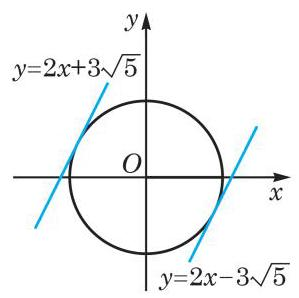
\includegraphics[max width=0.2\textwidth]{images/bo_d7fqvdc91nqc7381i9u0_46_198_570_299_298_0.jpg}
\end{center}
\hspace*{3em} 

图 2-1-5

当 \(\Delta  > 0\) ,即 \(- 3\sqrt{5} < b < 3\sqrt{5}\) 时,方程 \circled{3} 有两个不相等的实根,从而原方程组有两组不同的实数解,所以直线 \(l\) 与圆 \(C\) 有两个公共点.

当 \(\Delta  = 0\) ,即 \(b =  - 3\sqrt{5}\) 或 \(b = 3\sqrt{5}\) 时,方程 \circled{3} 有两个相等的实根,从而原方程组有两组相同的实数解,所以直线 \(l\) 与圆 \(C\) 只有一个公共点(图 2-1-5).

当 \(\Delta  < 0\) ,即 \(b <  - 3\sqrt{5}\) 或 \(b > 3\sqrt{5}\) 时,方程 \circled{3} 没有实根,从而原方程组没有实数解,所以直线 \(l\) 与圆 \(C\) 没有公共点.

解 (1) 因为 \(M\left( {{x}_{0},{y}_{0}}\right)\) 是 \(l\) 与圆 \(O\) 的切点,可知 \({x}_{0}^{2} + {y}_{0}^{2} = 4\) ,且过点 \(M\) 的半径 \({OM}\) 与 \(l\) 垂直,即 \(\overrightarrow{OM} = \left( {{x}_{0},{y}_{0}}\right)\) 是 \(l\) 的一个法向量,于是可得切线 \(l\) 的点法式方程为

\begin{center}
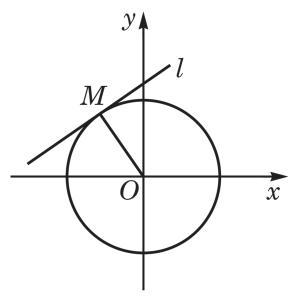
\includegraphics[max width=0.2\textwidth]{images/bo_d7fqvdc91nqc7381i9u0_46_200_1104_294_298_0.jpg}
\end{center}
\hspace*{3em} 

图 2-1-6

例 8 (1)如图2-1-6，已知 \(M\left( {{x}_{0},{y}_{0}}\right)\) 为圆 \(O\) : \({x}^{2} + {y}^{2} = 4\) 上一点,求过点 \(M\) 的圆 \(O\) 的切线 \(l\) 的方程;

(2)求过点 \(N\left( {2,2\sqrt{3}}\right)\) 且与圆 \(O : {x}^{2} + {y}^{2} = 4\) 相切的直线的方程.

\[
{x}_{0}\left( {x - {x}_{0}}\right)  + {y}_{0}\left( {y - {y}_{0}}\right)  = 0.
\]

整理, 得

\[
{x}_{0}x + {y}_{0}y = {x}_{0}^{2} + {y}_{0}^{2}.
\]

?

所以,过点 \(M\) 的圆 \(O\) 的切线 \(l\) 的方程为 \({x}_{0}x + {y}_{0}y = 4\) .

\HRule

请将例 8(1) 的结论加以推广, 使之成为推广后命题的一个特例.

\HRule

(2)由 \(\left| {ON}\right|  = \sqrt{{2}^{2} + {\left( 2\sqrt{3}\right) }^{2}} = 4\) ，知点 \(N\) 在已知圆 \(O\) 外.

先考虑过点 \(N\) 且具有斜率 \(k\) 的直线，可设其方程为

\[
y - 2\sqrt{3} = k\left( {x - 2}\right) \text{ ,即 }{kx} - y - {2k} + 2\sqrt{3} = 0.
\]

此直线与圆 \(O\) 相切当且仅当圆心 \(O\left( {0,0}\right)\) 到该直线的距离为 2 , 所以

\[
\frac{\left| -2k + 2\sqrt{3}\right| }{\sqrt{{k}^{2} + 1}} = 2\text{ ,即 }{\left( k - \sqrt{3}\right) }^{2} = {k}^{2} + 1\text{ , }
\]

解得 \(k = \frac{\sqrt{3}}{3}\) .

因此,得到过点 \(N\) 的圆 \(O\) 的一条切线,它的方程为

\[
\frac{\sqrt{3}}{3}x - y - \frac{2\sqrt{3}}{3} + 2\sqrt{3} = 0\text{ ,即 }x - \sqrt{3}y + 4 = 0\text{ . }
\]

?

过点 \(N\) 可以作圆 \(O\) 的两条切线,故另一条切线的斜率不存在,则其方程只能是 \(x = 2\) ,即 \(x - 2 = 0\) .

\HRule

我们还可以验证圆心到直线 \(x - 2 = 0\) 的距离等于半径 2 . 想一想, 这个验证是否必须?

\HRule

因此,所求直线的方程为 \(x - \sqrt{3}y + 4 = 0\) 或 \(x - 2 = 0\) .

\begin{center}
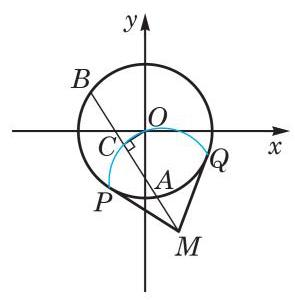
\includegraphics[max width=0.2\textwidth]{images/bo_d7fqvdc91nqc7381i9u0_47_1152_589_295_300_0.jpg}
\end{center}
\hspace*{3em} 

图 2-1-7

例 9 过圆 \(O : {x}^{2} + {y}^{2} = {16}\) 外一点 \(M\left( {2, - 6}\right)\) 任意作一条割线交圆 \(O\) 于 \(A\text{ 、 }B\) 两点,求弦 \({AB}\) 的中点 \(C\) 的轨迹.

解 如图 2-1-7,设弦 \({AB}\) 的中点 \(C\) 的坐标为 \(\left( {x,y}\right)\) ,连接 \({OC}\) . 可得 \(\overrightarrow{OC} \bot  \overrightarrow{AB}\) ,即 \(\overrightarrow{OC} \bot  \overrightarrow{MC}\) ,从而

\[
\overrightarrow{OC} \cdot  \overrightarrow{MC} = 0.
\]

又因为 \(\overrightarrow{OC} = \left( {x,y}\right) ,\overrightarrow{MC} = \left( {x - 2,y + 6}\right)\) ,

所以 \(x\left( {x - 2}\right)  + y\left( {y + 6}\right)  = 0\) ,即

\[
{\left( x - 1\right) }^{2} + {\left( y + 3\right) }^{2} = {10}.
\]

?

因此,点 \(C\) 的轨迹是以 \(\left( {1, - 3}\right)\) 为圆心、以 \(\sqrt{10}\) 为半径,且位于圆 \(O\) 内的一段圆弧 \(\overset{\text{ ⏜ }}{PQ}\) (图 2-1-7).

\HRule

例 9 还有其他解法吗?

\HRule

\section*{练习 2.1(3)}

1. ( 1 )求经过点 \(\left( {-3,4}\right)\) 且与圆 \({x}^{2} + {y}^{2} = {25}\) 相切的直线的方程；

(2)求经过点 \(\left( {2,4}\right)\) 且与圆 \({x}^{2} + {y}^{2} = 4\) 相切的直线的方程.

2. 当 \(a\) 为何值时,直线 \(x + y - a = 0\) 与圆 \({x}^{2} + {y}^{2} = 2\) 分别有如下位置关系:

(1)相交； (2)相切； (3)相离.

3. 已知直线 \(l\) 经过点 \(P\left( {6, - 4}\right)\) 且被圆 \({x}^{2} + {y}^{2} = {20}\) 截得长为 \(6\sqrt{2}\) 的弦,求 \(l\) 的方程.

\section*{5 圆与圆的位置关系}

圆是常见的平面几何图形, 两个或多个圆之间不同位置关系的合理使用, 会对装置的功能或艺术品的美感产生不同的作用. 如图 2-1-8 中的自行车双轮、滚珠轴承、奥运五环、花布图案, 都是圆的位置关系应用的实例.

\begin{center}
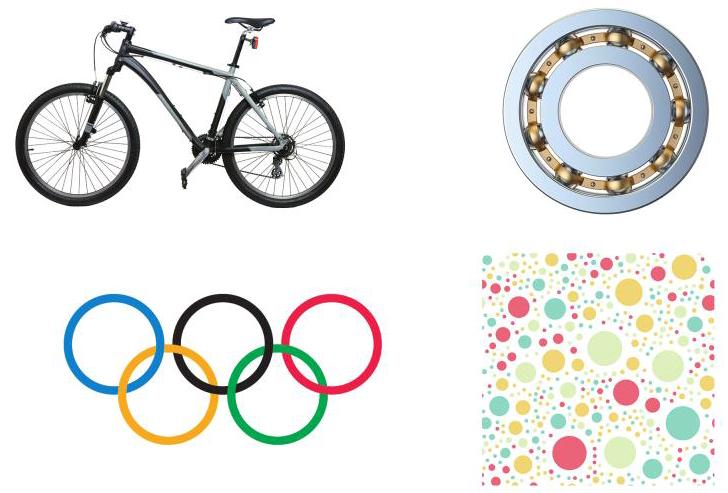
\includegraphics[max width=0.6\textwidth]{images/bo_d7fqvdc91nqc7381i9u0_48_636_241_728_493_0.jpg}
\end{center}
\hspace*{3em} 

图 2-1-8

我们只讨论两个圆的位置关系.

从初中的平面几何学习中, 我们知道两个圆之间有内含(包括同心)、内切、相交、外切和外离五种位置关系(当两个圆内含或内切时, 两个圆半径不相等). 在平面直角坐标系中, 如果给出两个圆的标准方程

\[
{C}_{1} : {\left( x - {a}_{1}\right) }^{2} + {\left( y - {b}_{1}\right) }^{2} = {r}_{1}^{2},
\]

\[
{C}_{2} : {\left( x - {a}_{2}\right) }^{2} + {\left( y - {b}_{2}\right) }^{2} = {r}_{2}^{2},
\]

我们就可以从方程中读出两个圆的圆心坐标 \(\left( {{a}_{1},{b}_{1}}\right) \text{ 、 }\left( {{a}_{2},{b}_{2}}\right)\) , 半径 \({r}_{1}\text{ 、 }{r}_{2}\) ,进而由圆心坐标求得圆心距

\[
d = \sqrt{{\left( {a}_{1} - {a}_{2}\right) }^{2} + {\left( {b}_{1} - {b}_{2}\right) }^{2}}.
\]

所以

当 \(d < \left| {{r}_{1} - {r}_{2}}\right|\) 时,两圆内含 \(\left( {{r}_{1} \neq  {r}_{2}}\right)\) ; 当 \(d = \left| {{r}_{1} - {r}_{2}}\right|\) 时,两圆内切 \(\left( {{r}_{1} \neq  {r}_{2}}\right)\) ; 当 \(\left| {{r}_{1} - {r}_{2}}\right|  < d < {r}_{1} + {r}_{2}\) 时,两圆相交; 当 \(d = {r}_{1} + {r}_{2}\) 时,两圆外切; 当 \(d > {r}_{1} + {r}_{2}\) 时,两圆外离.

如果给出两个圆的一般方程

\[
{C}_{1} : {x}^{2} + {y}^{2} + {D}_{1}x + {E}_{1}y + {F}_{1} = 0,
\]

\[
{C}_{2} : {x}^{2} + {y}^{2} + {D}_{2}x + {E}_{2}y + {F}_{2} = 0,
\]

我们当然可以把它们都化成标准方程, 然后用上述圆心距与半径的关系判断这两个圆的位置关系. 此外, 我们也可以像判断两条直线的位置关系与判断直线和圆的位置关系那样, 通过解联立方程组判断两个圆有几个公共点, 从而得知它们是相交、相切 (包括内切与外切) 还是相离 (包括内含与外离). 因此, 我们解方

程组

\[
\left\{  \begin{array}{l} {x}^{2} + {y}^{2} + {D}_{1}x + {E}_{1}y + {F}_{1} = 0, \\  {x}^{2} + {y}^{2} + {D}_{2}x + {E}_{2}y + {F}_{2} = 0. \end{array}\right.
\]

如果上述方程组有两组不同的解,那么圆 \({C}_{1}\) 与圆 \({C}_{2}\) 相交; 如果上述方程组只有一组解 (实际上应该理解为两组相同的解, 因为它们是由一元二次方程两个相同的根得出的),那么圆 \({C}_{1}\) 与圆 \({C}_{2}\) 内切或外切; 如果上述方程组无解,那么圆 \({C}_{1}\) 与圆 \({C}_{2}\) 内含或外离.

上述方程组由两个二元二次方程组成, 只要把这两个方程相减, 一般情况下可以得到一个二元一次方程

\[
\left( {{D}_{1} - {D}_{2}}\right) x + \left( {{E}_{1} - {E}_{2}}\right) y + \left( {{F}_{1} - {F}_{2}}\right)  = 0.
\]

因此, 求解上述方程组, 只要把这个二元一次方程和上述方程组中的任何一个方程联立求解就可以了.

例 10 判断圆 \({C}_{1} : {x}^{2} + {y}^{2} - {2x} = 0\) 与圆 \({C}_{2} : {x}^{2} + {y}^{2} - {4y} = 0\) 的位置关系.

解 联立方程组 \(\left\{  \begin{array}{l} {x}^{2} + {y}^{2} - {2x} = 0, \\  {x}^{2} + {y}^{2} - {4y} = 0. \end{array}\right.\) 将两方程相减并化简, 得 \(x = {2y}\) . 把它代入第一个方程得到 \(5{y}^{2} - {4y} = 0\) ,解得 \({y}_{1} = 0\) , \({y}_{2} = \frac{4}{5}\) ,从而 \({x}_{1} = 0,{x}_{2} = \frac{8}{5}\) .

所以,圆 \({C}_{1}\) 与圆 \({C}_{2}\) 相交于两点 \(\left( {0,0}\right) \text{ 、 }\left( {\frac{8}{5},\frac{4}{5}}\right)\) .

我们介绍了两种判断两个圆的位置关系的方法: 一是化成标准方程后利用两圆圆心距和半径的关系来判断；二是用解方程法求出公共点坐标后再判断. 两种方法各有利弊, 前者能够准确区分内切与外切、内含与外离, 但无法给出公共点坐标; 后者可以给出公共点坐标, 但无法区分内切与外切、内含与外离. 解题时应根据需要采用适当的方法, 或者两者并用, 求出所有需要的信息.

例 11 证明圆 \({C}_{1} : {x}^{2} + {y}^{2} - {4x} + {6y} + 5 = 0\) 与圆 \({C}_{2}\) : \({x}^{2} + {y}^{2} - {6x} + {4y} + {11} = 0\) 内切,并求切点坐标.

解 把两个方程都化成圆的标准方程:

\[
{C}_{1} : {\left( x - 2\right) }^{2} + {\left( y + 3\right) }^{2} = 8,
\]

\[
{C}_{2} : {\left( x - 3\right) }^{2} + {\left( y + 2\right) }^{2} = 2.
\]

这两个圆的圆心坐标分别是 \(\left( {2, - 3}\right)\) 与 \(\left( {3, - 2}\right)\) ,从而它们的圆心距是 \(d = \sqrt{{\left( 2 - 3\right) }^{2} + {\left( -3 + 2\right) }^{2}} = \sqrt{2}\) . 两个圆的半径分别是 \({r}_{1} = 2\sqrt{2}\) 与 \({r}_{2} = \sqrt{2}\) . 于是 \(d = \left| {{r}_{1} - {r}_{2}}\right|\) ,所以圆 \({C}_{1}\) 与圆 \({C}_{2}\) 内切.

\HRule

当 \({D}_{1} - {D}_{2}\) 与 \({E}_{1} - {E}_{2}\) 不同时为零时，二元一次方程 \(\left( {{D}_{1} - {D}_{2}}\right) x + \left( {{E}_{1} - }\right. \; \left. {E}_{2}\right) y + \left( {{F}_{1} - {F}_{2}}\right)  = 0\) 所表示的直线有什么几何意义吗?

当 \({D}_{1} - {D}_{2}\) 与 \({E}_{1} - {E}_{2}\) 同时为零时, 两圆有什么样的位置关系?

\HRule

把两个圆的方程相减并整理得 \(x = 3 - y\) . 代入圆 \({C}_{1}\) 的方程并化简得 \({y}^{2} + {2y} + 1 = 0\) . 这个一元二次方程有两个相同的根 \(y =  - 1\) ,从而 \(x = 4\) . 由此得到圆 \({C}_{1}\) 与圆 \({C}_{2}\) 的切点是 \(\left( {4, - 1}\right)\) .

例 12 如图 2-1-9(1)，圆 \({O}_{1}\) 与圆 \({O}_{2}\) 的半径都是 1， \({O}_{1}{O}_{2} = 4\) ,过动点 \(P\) 分别作圆 \({O}_{1}\) 、圆 \({O}_{2}\) 的切线 \({PM}\text{ 、 }{PN}(M\) 、 \(N\) 分别为切点),使得 \(\left| {PM}\right|  = \sqrt{2}\left| {PN}\right|\) . 试通过建立适当的平面直角坐标系,求动点 \(P\) 的轨迹.

\begin{center}
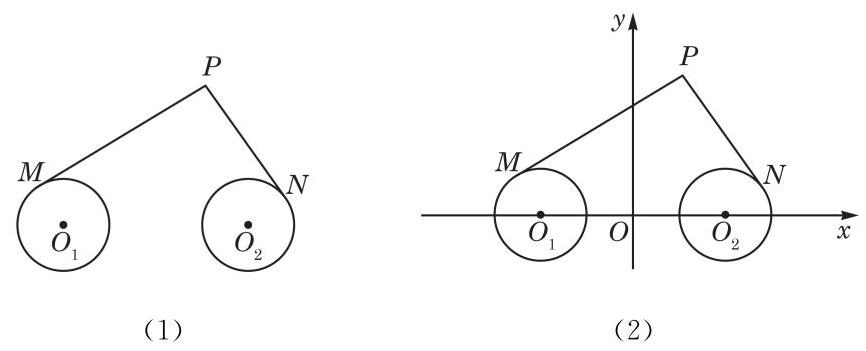
\includegraphics[max width=0.7\textwidth]{images/bo_d7fqvdc91nqc7381i9u0_50_591_929_866_351_0.jpg}
\end{center}
\hspace*{3em} 

图 2-1-9

解 如图 2-1-9(2),以 \({O}_{1}{O}_{2}\) 的中点 \(O\) 为原点, \({O}_{1}{O}_{2}\) 所在直线为 \(x\) 轴,以线段 \({O}_{1}{O}_{2}\) 的垂直平分线为 \(y\) 轴,建立平面直角坐标系,则 \({O}_{1}\) 的坐标为 \(\left( {-2,0}\right) ,{O}_{2}\) 的坐标为 \(\left( {2,0}\right)\) . 由 \(\left| {PM}\right|  = \sqrt{2}\left| {PN}\right|\) ,得 \({\left| PM\right| }^{2} = 2{\left| PN\right| }^{2}\) .

又因为两圆的半径均为 1,所以由勾股定理,得 \({\left| PM\right| }^{2} = \; {\left| P{O}_{1}\right| }^{2} - 1,{\left| PN\right| }^{2} = {\left| P{O}_{2}\right| }^{2} - 1\) ,从而 \({\left| P{O}_{1}\right| }^{2} - 1 = 2\left( {{\left| P{O}_{2}\right| }^{2} - 1}\right)\) .

设点 \(P\) 的坐标为 \(\left( {x,y}\right)\) ,则

\[
{\left( x + 2\right) }^{2} + {y}^{2} - 1 = 2\left\lbrack  {{\left( x - 2\right) }^{2} + {y}^{2} - 1}\right\rbrack  ,
\]

整理, 得

\[
{x}^{2} + {y}^{2} - {12x} + 3 = 0,
\]

Q

化为标准方程, 得

\[
{\left( x - 6\right) }^{2} + {y}^{2} = {33}.
\]

因此，所求的轨迹是以(6,0)为圆心、以 \(\sqrt{33}\) 为半径的圆.

\HRule

注意轨迹与轨迹的方程二者的区别与联系.

\HRule

\section*{练习 2.1(4)}

1. 已知圆 \({C}_{1} : {\left( x - 2\right) }^{2} + {\left( y - 2\right) }^{2} = 1\) 和圆 \({C}_{2} : {x}^{2} + {\left( y - m\right) }^{2} = {m}^{2}\left( {m > 0}\right)\) ,当 \(m\) 为何值时,圆 \({C}_{1}\) 与圆 \({C}_{2}\) 分别内切、相交?

2. 求与圆 \({x}^{2} + {y}^{2} = {25}\) 外切于点 \(P\left( {4, - 3}\right)\) 且半径为 1 的圆的方程.

3. 已知圆 \({x}^{2} + {y}^{2} - {2x} + {2y} - 3 = 0\) 和圆 \({x}^{2} + {y}^{2} + {4x} - 1 = 0\) 相交于 \(A\text{ 、 }B\) 两点,求公共弦 \({AB}\) 的长.

\section*{习题 2.1}

\section*{A 组}

1. 根据下列条件,分别求圆的方程:

(1)圆心为 \(C\left( {-\frac{3}{2},3}\right)\) ,半径 \(r = \sqrt{3}\) ；

(2)圆心为 \(C\left( {\sqrt{2},1}\right)\) ，过点 \(A\left( {-1,\sqrt{2}}\right)\) ；

(3)与 \(x\) 轴相交于 \(A\left( {1,0}\right)\) 、 \(B\left( {5,0}\right)\) 两点，且半径等于 \ding{51} 5.

2. 已知圆 \({\left( x - a\right) }^{2} + {\left( y - b\right) }^{2} = {r}^{2}\left( {r > 0}\right)\) ,求在下列情况下,实数 \(a\text{ 、 }b\text{ 、 }r\) 应分别满足什么条件:

(1)圆过原点； (2)圆心在 \(x\) 轴上；

(3)圆与 \(x\) 轴相切； (4)圆与两坐标轴均相切.

3. 求过点 \(M\left( {5,2}\right) \text{ 、 }N\left( {3,2}\right)\) ,且圆心在直线 \(y = {2x} - 3\) 上的圆的方程.

4. 已知 \({a}^{2}{x}^{2} + \left( {a + 2}\right) {y}^{2} + {2ax} + a = 0\) 表示圆,求实数 \(a\) 的值.

5. 直线 \(l\) 与圆 \({x}^{2} + {y}^{2} + {2x} - {4y} + a = 0\left( {a < 3}\right)\) 相交于 \(A\text{ 、 }B\) 两点,且弦 \({AB}\) 的中点为 \(\left( {0,1}\right)\) . 求直线 \(l\) 的方程.

6. 已知圆过原点，且与 \(x\) 轴、 \(y\) 轴的交点的坐标分别为 \(\left( {a,0}\right)\) 、 \(\left( {0,b}\right)\) ，其中 \({ab} \neq  0\) . 求这个圆的方程.

7. 判断直线 \(x\cos \theta  + y\sin \theta  = r\) 与圆 \({x}^{2} + {y}^{2} = {r}^{2}\) 的位置关系.

8. 已知直线 \({2x} + {3y} + 1 = 0\) 和圆 \({x}^{2} + {y}^{2} - {2x} - 3 = 0\) 相交于 \(A\text{ 、 }B\) 两点,求弦 \({AB}\) 的垂直平分线的方程.

9. 求与圆 \({x}^{2} + {y}^{2} = {25}\) 内切于点 \(P\left( {3, - 4}\right)\) 且半径为 1 的圆的方程.

10. 已知圆 \(C\) 过点 \(\left( {-4,0}\right)\) 且与圆 \({x}^{2} + {y}^{2} - {4x} - {6y} = 0\) 相切于原点,求圆 \(C\) 的方程.

11. 圆拱桥的一个圆拱如图所示,该圆拱的跨度 \({AB}\) 为 \({20}\mathrm{\;m}\) ,拱高 \({OP}\) 为 \(4\mathrm{\;m}\) ,在建造过程中每隔 \(4\mathrm{\;m}\) 需用一个支柱支撑. 求支柱 \({A}_{2}{B}_{2}\) 的高度. (结果精确到 \({0.01}\mathrm{\;m}\) )

\begin{center}
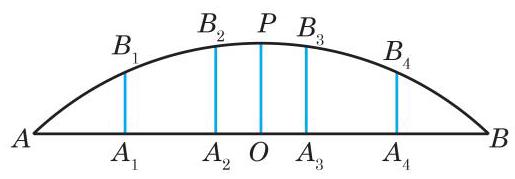
\includegraphics[max width=0.4\textwidth]{images/bo_d7fqvdc91nqc7381i9u0_52_580_346_515_179_0.jpg}
\end{center}
\hspace*{3em} 

(第 11 题)

\section*{B 组}

1. 给定点 \(A\left( {2,3}\right)\) 与圆 \(C : {x}^{2} + {y}^{2} = {25}\) ,求圆 \(C\) 的过点 \(A\) 最短弦所在直线的方程.

2. 一个圆过点 \(\left( {2, - 1}\right)\) ,圆心在直线 \({2x} + y = 0\) 上,且与直线 \(x - y - 1 = 0\) 相切. 求这个圆的方程.

3. 已知圆 \({x}^{2} + {y}^{2} + {6x} - {8y} + {25} = {r}^{2}\) 与 \(x\) 轴相切，求这个圆截 \(y\) 轴所得的弦长.

4. 求圆 \(C : {x}^{2} + {y}^{2} + {4x} + {2y} - 3 = 0\) 关于点 \(M\left( {1,1}\right)\) 对称的圆的方程.

5. 已知动直线 \({kx} - y + 1 = 0\) (其中 \(k \in  \mathbf{R}\) ) 和圆 \({x}^{2} + {y}^{2} = 4\) 相交于 \(A\text{ 、 }B\) 两点,求弦 \({AB}\) 的中点的轨迹方程.

6. 求经过点 \(\left( {5, - 5}\right)\) 且与圆 \({x}^{2} + {y}^{2} = {25}\) 相切的直线的方程.

7. 已知直线 \(y = x + m\) 和曲线 \(y = \sqrt{1 - {x}^{2}}\) 有两个不同的交点,求实数 \(m\) 的取值范围.

8. 已知直线 \(l : x - y + 4 = 0\) 与圆 \(C : {\left( x - 1\right) }^{2} + {\left( y - 1\right) }^{2} = 2\) ,求圆 \(C\) 上各点到直线 \(l\) 的距离的最大值.

9. 已知实数 \(x\text{ 、 }y\) 满足 \({\left( x - 2\right) }^{2} + {y}^{2} = 3\) ,求 \(\frac{y}{x}\) 的取值范围.

10. \({400}\mathrm{\;m}\) 标准跑道的内圈如图所示( \({400}\mathrm{\;m}\) 标准跑道最内圈的长度为 \({400}\mathrm{\;m}\) )，其中左右两端均是半径为 \({36}\mathrm{\;m}\) 的半圆弧.

(1)求每条直道的长度; ( \(\pi\) 取 3.14,结果精确到 \(1\mathrm{\;m}\) )

(2)建立适当的平面直角坐标系，写出上半部分跑道所对应的函数表达式.

\begin{center}
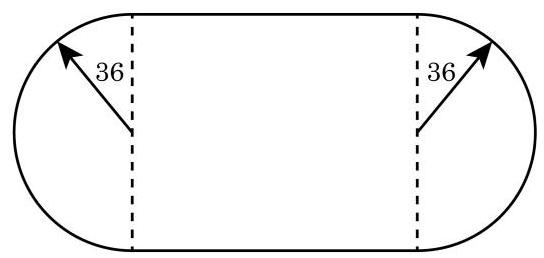
\includegraphics[max width=0.4\textwidth]{images/bo_d7fqvdc91nqc7381i9u0_52_567_1754_544_258_0.jpg}
\end{center}
\hspace*{3em} 

(第 10 题)

\section*{探究与实践}

\section*{追捕走私船}

如图 2-1-10,设直线 \(l\) 为公海与领海的分界线,一巡逻艇在 \(A\) 处发现北偏东 \({60}^{ \circ  }\) 海面 \(B\) 处有一艘走私船,此走私船正向停泊在公海上接应的走私海轮 \(C\) 航行,以便上海轮后逃窜. 已知巡逻艇的航速是走私船航速的 2 倍, \(A\) 与公海相距约 12 海里,走私船可能向任一方向逃窜. 请回答下列问题:

\begin{center}
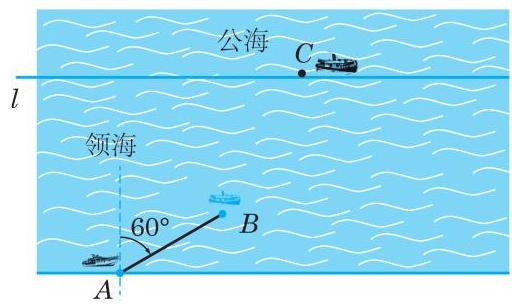
\includegraphics[max width=0.4\textwidth]{images/bo_d7fqvdc91nqc7381i9u0_53_549_787_512_306_0.jpg}
\end{center}
\hspace*{3em} 

图 2-1-10

(1)如果走私船和巡逻艇都是沿直线航行，那么走私船能被截获的点是哪些？

(2)根据截获点的轨迹，探讨“可截获区域”和“非截获区域”；

(3)如果走私船在非截获区域就进入公海，那么巡逻艇追捕失败. 要保证在领海内捕获,就应保证 “非截获区域”与公海区域不相交 (即交集为空集). 此时, \(A\text{ 、 }B\) 相距最远是多少海里?

\section*{2.2 椭圆}

\section*{1 椭圆的标准方程}

椭圆是一类重要的曲线. 早在 1609 年, 德国天文学家开普勒(J. Kepler)就提出了行星运动定律:每一个行星都沿各自的椭圆轨道环绕太阳转动, 而太阳则处在椭圆的一个焦点上. 生活中我们还可以在许多地方看到椭圆的形状, 如篮球在地面上的影子边界, 圆柱 (台) 形水杯倾斜时液面的边界线, 等等.

作为一条平面曲线, 椭圆有多种定义方式, 我们这里只给出其中的一种. 为此,先做一个简单的实验: 取一段长为 \({2a}\) 的绳子, 如果把这段绳子的两个端点分别固定在画图板上不同的两点 \({F}_{1}\) 和 \({F}_{2}\) 处,当绳长 \({2a} > \left| {{F}_{1}{F}_{2}}\right|\) 时,将铅笔尖套在绳子里并拉紧绳子,使笔尖 \(M\) 顺势移动一周,笔尖 \(M\) 画出来的图形就是一个椭圆 (图 2-2-1). 从上面的画图过程可以看出, 椭圆是由到两定点距离之和为定值的点所组成的集合.

\begin{center}
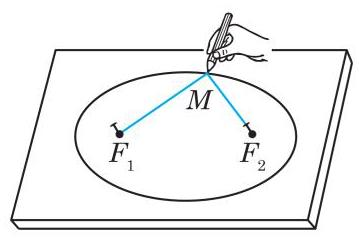
\includegraphics[max width=0.3\textwidth]{images/bo_d7fqvdc91nqc7381i9u0_54_164_1155_359_239_0.jpg}
\end{center}
\hspace*{3em} 

图 2-2-1

\begin{center}
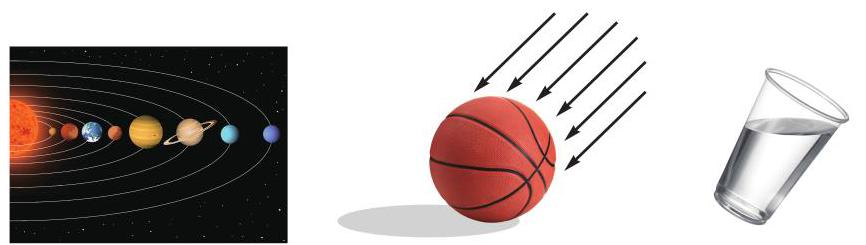
\includegraphics[max width=0.7\textwidth]{images/bo_d7fqvdc91nqc7381i9u0_54_586_1038_866_245_0.jpg}
\end{center}
\hspace*{3em} 

Q

\HRule

当点 \({F}_{1}\text{ 、 }{F}_{2}\) 重合时,点集 \(P\) 表示一个圆, 所以圆可以看作是椭圆的特殊情形. 但在本章中，除非特殊指出, 所说的椭圆均不包含圆这一特殊情形.

\HRule

我们把平面上到两个定点 \({F}_{1}\text{ 、 }{F}_{2}\) 的距离之和等于常数 \({2a} \; \left( {{2a} > \left| {{F}_{1}{F}_{2}}\right| }\right)\) 的点的轨迹叫做椭圆 (ellipse). 用集合的记号表示, 椭圆就是下述点集:

\[
P = \left\{  {M\left| \right| M{F}_{1}\left| +\right| M{F}_{2}\left| { = {2a},{2a} > }\right| {F}_{1}{F}_{2} \mid  }\right\}  .
\]

定点 \({F}_{1}\text{ 、 }{F}_{2}\) 叫做椭圆的焦点 (focus),两个焦点之间的距离 \(\left| {{F}_{1}{F}_{2}}\right|\) 叫做椭圆的焦距.

下面推导椭圆的方程.

以线段 \({F}_{1}{F}_{2}\) 的中点为原点,以 \(\overrightarrow{{F}_{1}{F}_{2}}\) 的方向为 \(x\) 轴的正方向, 建立如图 2-2-2 所示的平面直角坐标系. 设椭圆的焦距为 \({2c}\) ,则点 \({F}_{1}\text{ 、 }{F}_{2}\) 的坐标分别为 \(\left( {-c,0}\right) \text{ 、 }\left( {c,0}\right)\) .

\begin{center}
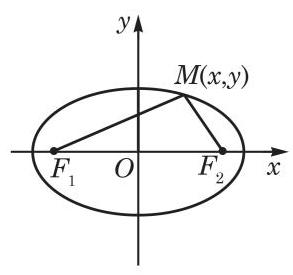
\includegraphics[max width=0.2\textwidth]{images/bo_d7fqvdc91nqc7381i9u0_55_1154_231_293_275_0.jpg}
\end{center}
\hspace*{3em} 

图 2-2-2

设点 \(M\left( {x,y}\right)\) 是椭圆上的任意一点,由定义有

\[
\left| {M{F}_{1}}\right|  + \left| {M{F}_{2}}\right|  = {2a}\left( {a > c > 0}\right) .
\]

因为 \(\left| {M{F}_{1}}\right|  = \sqrt{{\left( x + c\right) }^{2} + {y}^{2}},\left| {M{F}_{2}}\right|  = \sqrt{{\left( x - c\right) }^{2} + {y}^{2}}\) ,所以

\[
\sqrt{{\left( x + c\right) }^{2} + {y}^{2}} + \sqrt{{\left( x - c\right) }^{2} + {y}^{2}} = {2a},
\]

即

\[
\sqrt{{\left( x + c\right) }^{2} + {y}^{2}} = {2a} - \sqrt{{\left( x - c\right) }^{2} + {y}^{2}}.
\]

将上式两边平方, 得

\[
{\left( x + c\right) }^{2} + {y}^{2} = 4{a}^{2} - {4a}\sqrt{{\left( x - c\right) }^{2} + {y}^{2}} + {\left( x - c\right) }^{2} + {y}^{2}.
\]

整理, 得

\[
{a}^{2} - {cx} = a\sqrt{{\left( x - c\right) }^{2} + {y}^{2}}.
\]

两边再平方, 得

\[
{a}^{4} - 2{a}^{2}{cx} + {c}^{2}{x}^{2} = {a}^{2}{x}^{2} - 2{a}^{2}{cx} + {a}^{2}{c}^{2} + {a}^{2}{y}^{2}.
\]

整理, 得

\[
\left( {{a}^{2} - {c}^{2}}\right) {x}^{2} + {a}^{2}{y}^{2} = {a}^{2}\left( {{a}^{2} - {c}^{2}}\right) .
\]

因为 \(a > c > 0\) ,所以 \({a}^{2} - {c}^{2} > 0\) . 设 \({b}^{2} = {a}^{2} - {c}^{2}\) ,且 \(b > 0\) . 我们得到

\[
{b}^{2}{x}^{2} + {a}^{2}{y}^{2} = {a}^{2}{b}^{2},
\]

即

\[
\frac{{x}^{2}}{{a}^{2}} + \frac{{y}^{2}}{{b}^{2}} = 1\left( {a > b > 0}\right) .
\]
  \circled{1} 

上面的推导表明,椭圆上任意一点 \(M\) 的坐标 \(\left( {x,y}\right)\) 都是方程 \circled{1} 的解；反过来，可以证明以方程 \circled{1} 的解为坐标的点都在这个椭圆上(只需将上述推理过程反过来推演即可). 所以，方程 \circled{1} 就是这个椭圆的方程，它表示的是焦点在 \(x\) 轴上的椭圆.

如果所建立的平面直角坐标系使焦点 \({F}_{1}\text{ 、 }{F}_{2}\) 在 \(y\) 轴上，设点 \({F}_{1}\text{ 、 }{F}_{2}\) 的坐标分别为 \(\left( {0, - c}\right) \text{ 、 }\left( {0,c}\right)\) ,仍然设 \({b}^{2} = {a}^{2} - {c}^{2}\left( {b > 0}\right)\) , 只要将方程 \circled{1} 的 \(x\) 、 \(y\) 互换，那么所得椭圆(图 2-2-3)的方程为

\[
\frac{{y}^{2}}{{a}^{2}} + \frac{{x}^{2}}{{b}^{2}} = 1\left( {a > b > 0}\right) .
\]
  \circled{2} 

方程 \circled{1} 和 \circled{2} 都叫做椭圆的标准方程.

\begin{center}
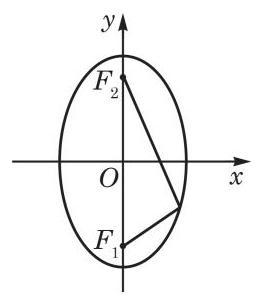
\includegraphics[max width=0.2\textwidth]{images/bo_d7fqvdc91nqc7381i9u0_55_1172_1754_256_301_0.jpg}
\end{center}
\hspace*{3em} 

图 2-2-3

例 1 已知椭圆的焦距是 6 , 椭圆上的一点到两个焦点的距离之和等于 10 . 求椭圆的标准方程.

解 因为 \(\left| {{F}_{1}{F}_{2}}\right|  = {2c} = 6,{2a} = {10}\) ,即 \(c = 3,a = 5\) ,所以

\[
{b}^{2} = {a}^{2} - {c}^{2} = {25} - 9 = {16}.
\]

当焦点在 \(x\) 轴上时,得椭圆的标准方程为

\[
\frac{{x}^{2}}{25} + \frac{{y}^{2}}{16} = 1
\]

?

当焦点在 \(y\) 轴上时,得椭圆的标准方程为

\[
\frac{{y}^{2}}{25} + \frac{{x}^{2}}{16} = 1
\]

\HRule

例 1 为什么有两种椭圆的标准方程?

\HRule

故椭圆的标准方程为 \(\frac{{x}^{2}}{25} + \frac{{y}^{2}}{16} = 1\) 或 \(\frac{{y}^{2}}{25} + \frac{{x}^{2}}{16} = 1\) .

例 2 求焦点在 \(x\) 轴上，焦距为 \(2\sqrt{6}\) ，且过点 \(\left( {\sqrt{3},\sqrt{2}}\right)\) 的椭圆的标准方程.

解 因为椭圆焦点在 \(x\) 轴上,所以设其方程为

\[
\frac{{x}^{2}}{{a}^{2}} + \frac{{y}^{2}}{{b}^{2}} = 1\left( {a > b > 0}\right) .
\]

由 \({2c} = 2\sqrt{6}\) ,得 \(c = \sqrt{6}\) ,因此

\[
{a}^{2} = {b}^{2} + 6\text{ . }
\]

又由于椭圆过点 \(\left( {\sqrt{3},\sqrt{2}}\right)\) ,因此

\[
\frac{3}{{a}^{2}} + \frac{2}{{b}^{2}} = 1
\]

求解上述二式组成的联立方程组,得 \({a}^{2} = 9,{b}^{2} = 3\) .

因此，所求椭圆的标准方程为 \(\frac{{x}^{2}}{9} + \frac{{y}^{2}}{3} = 1\) .

\section*{练习 2.2(1)}

1. 分别写出满足下列条件的动点 \(P\) 的轨迹方程:

(1)点 \(P\) 到点 \({F}_{1}\left( {-3,0}\right)\) 、 \({F}_{2}\left( {3,0}\right)\) 的距离之和为 10 ；

(2)点 \(P\) 到点 \({F}_{1}\left( {0, - 2}\right)\) 、 \({F}_{2}\left( {0,2}\right)\) 的距离之和为 12；

(3)点 \(P\) 到点 \({F}_{1}\left( {-4,0}\right)\) 、 \({F}_{2}\left( {4,0}\right)\) 的距离之和为 8 .

2. 分别写出满足下列条件的椭圆的标准方程:

(1)焦点在 \(y\) 轴上，焦距为 \(2\sqrt{15}\) ，且经过点 \(\left( {0, - 4}\right)\) ；

(2)焦距为 4，且经过点 \(\left( {\sqrt{5},0}\right)\) .

\section*{2 椭圆的性质}

在解析几何中, 可利用曲线的方程研究曲线的几何性质. 我们从椭圆的标准方程

\[
\frac{{x}^{2}}{{a}^{2}} + \frac{{y}^{2}}{{b}^{2}} = 1\left( {a > b > 0}\right)
\]
  \circled{1} 

出发, 可以得到椭圆的下列性质.

\section*{(1)对称性}

从椭圆的形状上看, 椭圆有两条相互垂直的对称轴. 这里, 也可以通过方程 \circled{1} 讨论椭圆的对称性. 容易验证,如果点 \({M}_{1}\left( {x,y}\right)\) 的坐标满足方程 \circled{1} ，那么它关于 \(y\) 轴的对称点 \({M}_{2}\left( {-x,y}\right)\) 、关于 \(x\) 轴的对称点 \({M}_{3}\left( {x, - y}\right)\) 及关于坐标原点的对称点 \({M}_{4}\left( {-x, - y}\right)\) 的坐标也都满足方程 \circled{1} (图 2-2-4)，所以椭圆关于 \(y\) 轴、 \(x\) 轴和坐标原点对称. 因此, 椭圆既是轴对称图形, 有两条互相垂直的对称轴; 也是中心对称图形, 其唯一的对称中心叫做椭圆的中心.

\begin{center}
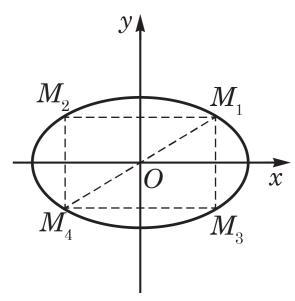
\includegraphics[max width=0.2\textwidth]{images/bo_d7fqvdc91nqc7381i9u0_57_1152_912_295_301_0.jpg}
\end{center}
\hspace*{3em} 

图 2-2-4

\section*{(2) 顶点}

\begin{center}
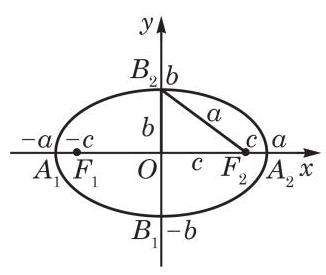
\includegraphics[max width=0.2\textwidth]{images/bo_d7fqvdc91nqc7381i9u0_57_1138_1428_326_275_0.jpg}
\end{center}
\hspace*{3em} 

图 2-2-5

如图 2-2-5, 椭圆与它的对称轴的交点叫做椭圆的顶点 (vertex).

在方程 \circled{1} 中，令 \(y = 0\) ，得 \(x =  \pm  a\) ；令 \(x = 0\) ，得 \(y =  \pm  b\) . 所以椭圆与两条坐标轴的交点分别是 \({A}_{1}\left( {-a,0}\right) \text{ 、 }{A}_{2}\left( {a,0}\right)\) 、 \({B}_{1}\left( {0, - b}\right) \text{ 、 }{B}_{2}\left( {0,b}\right)\) . 这四个点都是椭圆的顶点.

因为 \(a > b > 0\) ,我们把线段 \({A}_{1}{A}_{2}\) 叫做椭圆的长轴 (long axis), 长轴的长等于 \({2a}\) ; 线段 \({B}_{1}{B}_{2}\) 叫做椭圆的短轴 (short axis),短轴的长等于 \({2b}\) . 方便起见,把 \(a\) 和 \(b\) 分别称为椭圆的长半轴的长和短半轴的长. 椭圆的焦距为 \({2c}\) ,椭圆的半焦距为 \(c\) . 椭圆的两个焦点都在它的长轴上. 由于 \({a}^{2} = {b}^{2} + {c}^{2}\) ,焦点和短半轴顶点的距离就等于长半轴的长 (图 2-2-5).

由椭圆的对称性知, 椭圆的长轴和短轴分别所在的直线就是椭圆的两条对称轴.

\section*{(3)范围}

由方程 \circled{1} 可知,椭圆上每一点的坐标 \(\left( {x,y}\right)\) 都满足不等式

\[
\frac{{x}^{2}}{{a}^{2}} \leq  1,\frac{{y}^{2}}{{b}^{2}} \leq  1,
\]

\begin{center}
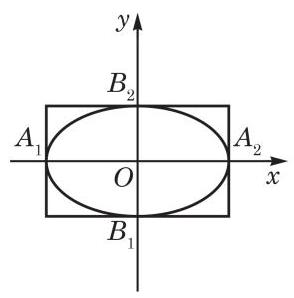
\includegraphics[max width=0.2\textwidth]{images/bo_d7fqvdc91nqc7381i9u0_58_201_404_294_298_0.jpg}
\end{center}
\hspace*{3em} 

图 2-2-6

即

\[
- a \leq  x \leq  a,\; - b \leq  y \leq  b.
\]

这说明椭圆位于直线 \(x =  \pm  a\) 和直线 \(y =  \pm  b\) 所围成的矩形内(图 2-2-6).

\section*{(4)离心率}

椭圆的焦距与长轴长的比 \(e = \frac{c}{a}\) ,叫做椭圆的离心率 (eccentricity).

因为 \(a > c > 0\) ,所以 \(0 < e < 1\) . 在 \(a\) 确定的条件下, \(e\) 越接近于 1,则 \(c\) 越接近于 \(a\) ,从而 \(b = \sqrt{{a}^{2} - {c}^{2}}\) 越小,因此椭圆越扁; 反之, \(e\) 越接近于 0,则 \(c\) 越接近于 0,从而 \(b\) 越接近于 \(a\) ,这时椭圆就越接近于圆. Q

\HRule

\(a = b\) 时, \(c = 0\) , 这时两个焦点重合于椭圆的中心，椭圆变为圆, 其方程为 \({x}^{2} + {y}^{2} = {a}^{2}.\)

\HRule

例 3 求椭圆 \(9{x}^{2} + {25}{y}^{2} = {225}\) 的长轴和短轴的长、离心率以及焦点和顶点的坐标.

解 将给定的椭圆方程化成标准方程

\[
\frac{{x}^{2}}{25} + \frac{{y}^{2}}{9} = 1
\]

这里 \(a = 5,b = 3,c = \sqrt{{a}^{2} - {b}^{2}} = 4\) .

所以，椭圆的长轴和短轴的长分别是 10 和 6，离心率 \(e = \frac{c}{a} = \frac{4}{5}\) ， 两个焦点在 \(x\) 轴上,它们的坐标分别是 \(\left( {-4,0}\right)\) 和 \(\left( {4,0}\right)\) ,四个顶点的坐标分别是 \(\left( {-5,0}\right) \text{ 、 }\left( {5,0}\right) \text{ 、 }\left( {0, - 3}\right) \text{ 、 }\left( {0,3}\right)\) .

\section*{练习 2.2(2)}

1. 已知下列椭圆的方程，分别求椭圆的长轴长、短轴长、焦点坐标和顶点坐标:

(1) \(\frac{{x}^{2}}{4} + \frac{{y}^{2}}{3} = 1\) ；\_\_\_\_\_ (2) \({25}{x}^{2} + 4{y}^{2} = {100}\) .

2. 用离心率作为指标衡量, 下列每组两个椭圆中哪一个更接近圆?

(1) \(\frac{{x}^{2}}{4} + \frac{{y}^{2}}{9} = 1\) 与 \(\frac{{x}^{2}}{16} + \frac{{y}^{2}}{12} = 1\) ；

(2) \({x}^{2} + 9{y}^{2} = {36}\) 与 \(5{x}^{2} + 3{y}^{2} = {30}\) .

3. 若一椭圆以原点为中心，一个焦点的坐标为 \(\left( {\sqrt{2},0}\right)\) ，且长轴长是短轴长的。 \(\sqrt{3}\) 倍. 求该椭圆的标准方程.

例 4 我国发射的第一颗人造地球卫星, 它的运行轨道是以地球的中心 \({F}_{2}\) 为一个焦点的椭圆,椭圆长轴的两个端点 \(A\) 、 \(B\) 分别为近地点和远地点,如图 2-2-7 所示. 卫星在近地点 \(A\) 与地球表面的距离约为 \({440}\mathrm{\;{km}}\) ,在远地点 \(B\) 与地球表面的距离约为 \({2384}\mathrm{\;{km}}\) ,地球中心与 \(A\text{ 、 }B\) 在同一直线上. 已知地球的半径 \(R\) 约为 \({6371}\mathrm{\;{km}}\) . 以 \(\mathrm{{km}}\) 为单位,建立适当的平面直角坐标系, 求卫星轨道的方程. (结果精确到 \(1\mathrm{\;{km}}\) )

\begin{center}
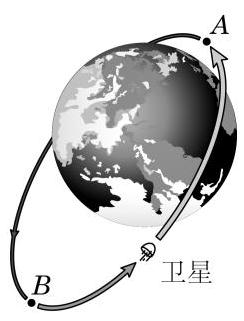
\includegraphics[max width=0.2\textwidth]{images/bo_d7fqvdc91nqc7381i9u0_59_1161_479_244_321_0.jpg}
\end{center}
\hspace*{3em} 

图 2-2-7

解 如图 2-2-8,以卫星轨道的中心 \(O\) 为原点,线段 \({AB}\) 所在的直线为 \(x\) 轴, \(\overrightarrow{OA}\) 方向为 \(x\) 轴的正方向,建立平面直角坐标系. 因焦点 \({F}_{2}\) 在 \(x\) 轴正半轴上,可设地球的中心为 \({F}_{2}\left( {c,0}\right)\) , 所求卫星轨道的方程为

\[
\frac{{x}^{2}}{{a}^{2}} + \frac{{y}^{2}}{{b}^{2}} = 1\left( {a > b > 0}\right) .
\]

\HRule

为什么近地点和远地点分别在椭圆的长轴的两个端点处?

\HRule

\begin{center}
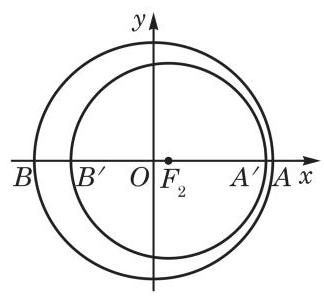
\includegraphics[max width=0.2\textwidth]{images/bo_d7fqvdc91nqc7381i9u0_59_1139_1113_324_299_0.jpg}
\end{center}
\hspace*{3em} 

图 2-2-8

设 \({A}^{\prime }\text{ 、 }{B}^{\prime }\) 是 \({AB}\) 与地球表面的两个交点. 因为

\[
a - c = \left| {A{F}_{2}}\right|  = \left| {A{A}^{\prime }}\right|  + R = {440} + {6371} = {6811},
\]

\[
a + c = \left| {B{F}_{2}}\right|  = \left| {B{B}^{\prime }}\right|  + R = {2384} + {6371} = {8755},
\]

所以

\[
a = {7783},c = {972}.
\]

从而

\[
b = \sqrt{{a}^{2} - {c}^{2}} \approx  {7722}.
\]

因此,所求卫星轨道的方程为 \(\frac{{x}^{2}}{{7783}^{2}} + \frac{{y}^{2}}{{7723}^{2}} = 1\) .

\begin{center}
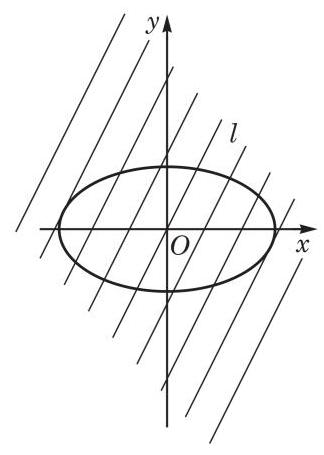
\includegraphics[max width=0.2\textwidth]{images/bo_d7fqvdc91nqc7381i9u0_59_1135_1594_324_455_0.jpg}
\end{center}
\hspace*{3em} 

图 2-2-9

例 5 设直线与椭圆的方程分别为 \({2x} - y = b\) 与 \(\frac{{x}^{2}}{75} + \frac{{y}^{2}}{25} = 1\) ,当 \(b\) 为何值时,它们满足下列关系:

(1)直线与椭圆有且只有一个公共点；

(2)直线与椭圆有两个公共点；

(3)直线与椭圆没有公共点.

解 如图 2-2-9,当 \(b\) 变化时,方程 \({2x} - y = b\) 表示的是斜率为 2 的一组平行线. 由直线的方程得 \(y = {2x} - b\) ,代入椭圆的方程后整理得

\[
{13}{x}^{2} - {12bx} + 3{b}^{2} - {75} = 0.
\]

此一元二次方程根的判别式

\[
\Delta  = {\left( -{12}b\right) }^{2} - 4 \times  {13}\left( {3{b}^{2} - {75}}\right)  = {12}\left( {{325} - {b}^{2}}\right) .
\]

由此可知:

(1)当 \(\Delta  = 0\) ，即 \(b =  \pm  \sqrt{325} =  \pm  5\sqrt{13}\) 时，直线与椭圆只有一个公共点.

(2)当 \(\Delta  > 0\) ，即 \(- 5\sqrt{13} < b < 5\sqrt{13}\) 时，直线与椭圆有两个公共点.

Q

(3)当 \(\Delta  < 0\) ，即 \(b > 5\sqrt{13}\) 或 \(b <  - 5\sqrt{13}\) 时，直线与椭圆没有公共点.

\HRule

椭圆的切线具有下面的光学性质: 从椭圆的一个焦点发出的光线在到达椭圆上后, 被经过到达点的切线反射后必经过椭圆的另一个焦点. 椭圆的这一光学性质在医学等领域有广泛的应用。

\HRule

例 5 中的 (1), 直线与椭圆有且只有一个公共点. 一般地, 如果一条直线与一个椭圆有且只有一个公共点, 就说这条直线与这个椭圆相切, 这条直线称为这个椭圆的切线. 显然, 如果椭圆的标准方程是 \(\frac{{x}^{2}}{{a}^{2}} + \frac{{y}^{2}}{{b}^{2}} = 1\left( {a > b > 0}\right)\) ,那么直线 \(x =  \pm  a,y =  \pm  b\) 都是这个椭圆的切线, 其切点分别为椭圆的四个顶点.

\section*{练习 2.2(3)}

1. 已知 \(P\) 是椭圆 \(\frac{{x}^{2}}{36} + \frac{{y}^{2}}{20} = 1\) 上一个动点, \({F}_{1}\) 是椭圆的左焦点. 求 \(\left| {P{F}_{1}}\right|\) 的最大值和最小值.

2. 点 \(P\) 在焦点为 \({F}_{1}\text{ 、 }{F}_{2}\) 的椭圆 \(\frac{{x}^{2}}{45} + \frac{{y}^{2}}{20} = 1\) 上,且 \(\angle {F}_{1}P{F}_{2} = {90}^{ \circ  }\) . 求 \(\left| {P{F}_{1}}\right|  \cdot  \left| {P{F}_{2}}\right|\) 的值.

3. 已知直线 \(l : y = {mx} - 2\) 与椭圆 \(C : \frac{{x}^{2}}{4} + \frac{{y}^{2}}{3} = 1\) 相交于两个不同的点,求实数 \(m\) 的取值范围.

\section*{习题 2.2}

\section*{A 组}

1. 若方程 \({16}{x}^{2} + k{y}^{2} = {16k}\) 表示焦点在 \(y\) 轴上的椭圆,求实数 \(k\) 的取值范围.

2. 设 \(F\) 是椭圆的一个焦点, \({B}_{1}{B}_{2}\) 是椭圆的短轴, \(\angle {B}_{1}F{B}_{2} = {60}^{ \circ  }\) . 求椭圆的离心率.

3. 已知椭圆的一个焦点是 \({F}_{1}\left( {-3,0}\right)\) ，且经过点 \(P\left( {2,\sqrt{2}}\right)\) . 求这个椭圆的标准方程.

4. 直线 \(y = {2x} + b\) 被椭圆 \(4{x}^{2} + {y}^{2} = {16}\) 所截得的弦长为 \(\sqrt{35}\) ，求实数 \(b\) 的值.

5. 若对于任意实数 \(k\) ,直线 \(y = {kx} + 1\) 与椭圆 \(\frac{{x}^{2}}{5} + \frac{{y}^{2}}{m} = 1\) 恒有公共点. 求实数 \(m\) 的取值范围.

B 组

1. 已知 \(P\) 是椭圆 \(\frac{{x}^{2}}{25} + \frac{{y}^{2}}{9} = 1\) 上的点， \({F}_{1}\) 、 \({F}_{2}\) 是椭圆的两个焦点.

(1)若 \(\angle {F}_{1}P{F}_{2} = {60}^{ \circ  }\) ，求 \(\bigtriangleup P{F}_{1}{F}_{2}\) 的面积；

(2)若 \(\bigtriangleup P{F}_{1}{F}_{2}\) 的面积为 9，求 \(\angle {F}_{1}P{F}_{2}\) 的大小.

2. 水星的运行轨道是以太阳的中心为一个焦点的椭圆, 轨道上离太阳中心最近的距离约为 \({4.7} \times  {10}^{8}\mathrm{\;{km}}\) ,最远的距离约为 \({7.05} \times  {10}^{8}\mathrm{\;{km}}\) . 以这个轨道的中心为原点,以太阳中心及轨道中心所在直线为 \(x\) 轴,建立平面直角坐标系. 求水星运行轨道的方程. (长半轴的长和短半轴的长精确到 \({0.1} \times  {10}^{8}\mathrm{\;{km}}\) )

\section*{2.3 双曲线}

\section*{1 双曲线的标准方程}

如图 2-3-1,给定两个定点 \({F}_{1}\) 与 \({F}_{2}\) ,将一条拉链先拉开一部分,并将拉开的一支的一端固定在 \({F}_{2}\) 处,在另一支上选择一点固定在 \({F}_{1}\) 处,在拉链头 \(M\) 处放上一支铅笔,然后逐渐拉开拉链,让铅笔尖 \(M\) 顺势移动,则笔尖 \(M\) 画出的图形 (图 2-3-2 中实线所示的曲线在直线 \({F}_{1}{F}_{2}\) 上方的部分) 就是使 \(\left| {M{F}_{2}}\right|  - \left| {M{F}_{1}}\right|\) 为常数 \(\left| {P{F}_{1}}\right|\) 的点 \(M\) 的轨迹的一部分.

\begin{center}
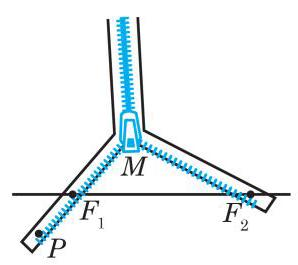
\includegraphics[max width=0.2\textwidth]{images/bo_d7fqvdc91nqc7381i9u0_62_198_752_298_265_0.jpg}
\end{center}
\hspace*{3em} 

图 2-3-1

我们知道平面上到两个定点的距离之和等于常数 (此常数大于两定点之间的距离) 的点的轨迹是椭圆, 那么平面上到两个定点的距离之差等于常数的点的轨迹是怎样的曲线呢?

\begin{center}
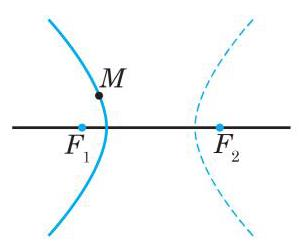
\includegraphics[max width=0.2\textwidth]{images/bo_d7fqvdc91nqc7381i9u0_62_198_1201_299_248_0.jpg}
\end{center}
\hspace*{3em} 

图 2-3-2

如果把拉链想象成无限长,那么得到的点 \(M\) 的轨迹就向上方无限伸展了; 如果把拉链翻转 \({180}^{ \circ  }\) ,又可以画出图 2-3-2 中实线所示的曲线在直线 \({F}_{1}{F}_{2}\) 下方的部分. 交换 \(M{F}_{1}\) 与 \(M{F}_{2}\) 的长度, 图中用虚线表示的曲线也可用类似方法画出.

我们把平面上到两个定点 \({F}_{1}\text{ 、 }{F}_{2}\) 的距离之差的绝对值等于常数 \({2a}\left( {0 < {2a} < \left| {{F}_{1}{F}_{2}}\right| }\right)\) 的点的轨迹叫做双曲线 (hyperbola). 双曲线也可表示为如下点集:

?

\[
P = \left\{  {M\left| \right| \left| {M{F}_{1}}\right|  - \left| {M{F}_{2}}\right|  \mid   = {2a},0 < {2a} < \left| {{F}_{1}{F}_{2}}\right| }\right\}  .
\]

\HRule

为什么要加条件: “绝对值”? 为什么要加条件: \(0 < {2a} < \; \left| {{F}_{1}{F}_{2}}\right|\) ?

\HRule

定点 \({F}_{1}\text{ 、 }{F}_{2}\) 叫做双曲线的焦点,两个焦点之间的距离 \(\left| {{F}_{1}{F}_{2}}\right|\) 叫做双曲线的焦距.

\begin{center}
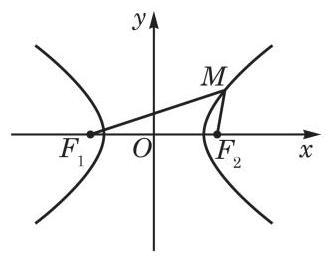
\includegraphics[max width=0.2\textwidth]{images/bo_d7fqvdc91nqc7381i9u0_62_185_1835_327_259_0.jpg}
\end{center}
\hspace*{3em} 

图 2-3-3

下面根据双曲线的定义, 参照求椭圆的方程的方法推导双曲线的方程.

取线段 \({F}_{1}{F}_{2}\) 的中点为原点, \(\overrightarrow{{F}_{1}{F}_{2}}\) 的方向为 \(x\) 轴的正方向, 建立平面直角坐标系, 如图 2-3-3 所示. 设两个焦点之间的距离 \(\left| {{F}_{1}{F}_{2}}\right|  = {2c}\left( {0 < a < c}\right)\) ,则点 \({F}_{1}\text{ 、 }{F}_{2}\) 的坐标分别是 \(\left( {-c,0}\right) \text{ 、 }\left( {c,0}\right)\) .

设 \(M\left( {x,y}\right)\) 是双曲线上的任意一点,由定义,有

\[
\left| \right| M{F}_{1}\left| -\right| M{F}_{2}\left| \right|  = {2a}\left( {c > a > 0}\right) .
\]

因为 \(\left| {M{F}_{1}}\right|  = \sqrt{{\left( x + c\right) }^{2} + {y}^{2}},\left| {M{F}_{2}}\right|  = \sqrt{{\left( x - c\right) }^{2} + {y}^{2}}\) , 所以

\[
\left| {\sqrt{{\left( x + c\right) }^{2} + {y}^{2}} - \sqrt{{\left( x - c\right) }^{2} + {y}^{2}}}\right|  = {2a},
\]

即

\[
\sqrt{{\left( x + c\right) }^{2} + {y}^{2}} = \sqrt{{\left( x - c\right) }^{2} + {y}^{2}} \pm  {2a}.
\]

将上式两边平方, 并整理后可得

\[
{cx} - {a}^{2} =  \pm  a\sqrt{{\left( x - c\right) }^{2} + {y}^{2}}.
\]

再将上式两边平方, 并整理后可得

\[
\left( {{c}^{2} - {a}^{2}}\right) {x}^{2} - {a}^{2}{y}^{2} = {a}^{2}\left( {{c}^{2} - {a}^{2}}\right) .
\]

因为 \(c > a > 0\) ,所以 \({c}^{2} - {a}^{2} > 0\) . 从而可令 \({b}^{2} = {c}^{2} - {a}^{2}\left( {b > 0}\right)\) , 并将上式改写为

\[
\frac{{x}^{2}}{{a}^{2}} - \frac{{y}^{2}}{{b}^{2}} = 1\left( {a > 0,b > 0}\right) .
\]
  \circled{1} 

因此,双曲线上任意一点 \(M\) 的坐标 \(\left( {x,y}\right)\) 都是方程 \circled{1} 的解. 反过来, 可以证明以方程 \circled{1} 的解为坐标的点都在这个双曲线上(只需将上述推理过程反过来推演即可).

方程 \circled{1} 所表示的双曲线的焦点在 \(x\) 轴上,且坐标分别为 \({F}_{1}\left( {-c,0}\right) \text{ 、 }{F}_{2}\left( {c,0}\right)\) ,而 \({c}^{2} = {a}^{2} + {b}^{2}\) . 如图 2-3-3,双曲线由两支分开的曲线组成.

如果以连接两个焦点 \({F}_{1}\) 和 \({F}_{2}\) 的直线为 \(y\) 轴,线段 \({F}_{1}{F}_{2}\) 的垂直平分线为 \(x\) 轴,如图 2-3-4 所示,那么两个焦点可分别设为 \({F}_{1}\left( {0, - c}\right) \text{ 、 }{F}_{2}\left( {0,c}\right)\) ,此时只要将方程 \circled{1} 的 \(x\text{ 、 }y\) 互换,就可得双曲线的方程是

\[
\frac{{y}^{2}}{{a}^{2}} - \frac{{x}^{2}}{{b}^{2}} = 1\left( {a > 0,b > 0}\right) ,
\]
  \circled{2} 

\begin{center}
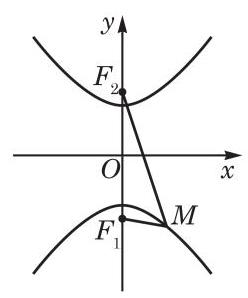
\includegraphics[max width=0.2\textwidth]{images/bo_d7fqvdc91nqc7381i9u0_63_1177_1468_248_298_0.jpg}
\end{center}
\hspace*{3em} 

图 2-3-4

其中, \(a\text{ 、 }b\text{ 、 }c\) 的关系仍是 \({c}^{2} = {a}^{2} + {b}^{2}\) .

方程 \circled{1} 和 \circled{2} 都叫做双曲线的标准方程.

例 1 已知双曲线的焦距是 6 , 双曲线上的点到两个焦点距离之差的绝对值等于 4 . 写出双曲线的标准方程和焦点的坐标.

解 因为 \({2c} = 6,{2a} = 4\) ,即 \(c = 3,a = 2\) ,所以

\[
{b}^{2} = {c}^{2} - {a}^{2} = 9 - 4 = 5\text{ . }
\]

于是,焦点在 \(x\) 轴上的双曲线的标准方程是 \(\frac{{x}^{2}}{4} - \frac{{y}^{2}}{5} = 1\) ,它的两个焦点的坐标是 \(\left( {-3,0}\right)\) 和 \(\left( {3,0}\right)\) .

焦点在 \(y\) 轴上的双曲线的标准方程是 \(\frac{{y}^{2}}{4} - \frac{{x}^{2}}{5} = 1\) ,它的两个焦点的坐标是 \(\left( {0, - 3}\right)\) 和 \(\left( {0,3}\right)\) .

例 2 已知点 \(M\left( {x,y}\right)\) 到点 \({F}_{1}\left( {-3,0}\right)\) 的距离减去它到点 \({F}_{2}\left( {3,0}\right)\) 的距离之差是 \(m\) ,分别求下列条件下点 \(M\) 的轨迹方程:

?

(1) \(m = 4\) ； (2) \(m = 6\) .

\HRule

例 2(1) 中,点 \(M\) 的轨迹为什么只是双曲线的右支?

\HRule

解(1)依题意，

\[
\left| {M{F}_{1}}\right|  - \left| {M{F}_{2}}\right|  = 4.
\]

而 \(4 < \left| {{F}_{1}{F}_{2}}\right|  = 6\) ,所以点 \(M\) 的轨迹是以 \({F}_{1}\text{ 、 }{F}_{2}\) 为焦点的双曲线的右支,且 \(c = 3,a = 2\) .

因为 \({b}^{2} = {c}^{2} - {a}^{2} = 5\) ,所以点 \(M\) 的轨迹方程为 \(\frac{{x}^{2}}{4} - \frac{{y}^{2}}{5} = 1\left( {x \geq  2}\right)\) .

(2)当 \(m = 6\) 时， \(\left| {M{F}_{1}}\right|  - \left| {M{F}_{2}}\right|  = \left| {{F}_{1}{F}_{2}}\right|\) ，此时点 \(M\) 的轨迹是以 \({F}_{2}\) 为端点在 \(x\) 轴上向正方向的射线,轨迹方程为 \(y = 0\left( {x \geq  3}\right)\) .

\begin{center}
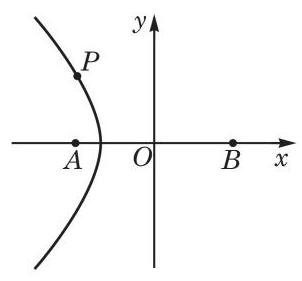
\includegraphics[max width=0.2\textwidth]{images/bo_d7fqvdc91nqc7381i9u0_64_197_1276_302_281_0.jpg}
\end{center}
\hspace*{3em} 

图 2-3-5

例 3 在相距 2000 m 的两个观察站 \(A\) 、 \(B\) 先后听到远处传来的爆炸声,已知 \(A\) 站听到的时间比 \(B\) 站早 \(4\mathrm{\;s}\) ,声速是 340 m/s. 建立适当的平面直角坐标系, 判断爆炸点可能分布在什么样的轨迹上, 并求该轨迹的方程.

解 设爆炸点为 \(P\) ,由题意知

\[
\left| {PB}\right|  - \left| {PA}\right|  = {340} \times  4 = {1360}.
\]

\[
\left| {AB}\right|  = {2000} > {1360},
\]

又

Q

所以点 \(P\) 分布在以 \(A\text{ 、 }B\) 为焦点的双曲线且靠近 \(A\) 处的一支上.

\HRule

双曲线具有很好的定位功能. 航海中使用的就是一种双曲线定位系统. 这一系统是由设置在岸上的两个发射台以及船上的接收机(定位仪)等组成, 通过测定两个发射台发射的电磁波传播到船上的时差来确定船舶的位置.

\HRule

如图 2-3-5,以 \({AB}\) 的中点为原点,以 \(\overrightarrow{AB}\) 的方向为 \(x\) 轴正方向,且以 \(\mathrm{m}\) 为单位,建立平面直角坐标系.

由 \(\left| {AB}\right|  = {2c} = {2000},\left| {PB}\right|  - \left| {PA}\right|  = {2a} = {1360}\) ,得

\[
c = {1000},a = {680},
\]

\[
{b}^{2} = {c}^{2} - {a}^{2} = {1000}^{2} - {680}^{2} = {537600}.
\]

所以,点 \(P\) 所在的轨迹的方程为 \(\frac{{x}^{2}}{462400} - \frac{{y}^{2}}{537600} = 1\left( {x \leq   - {680}}\right)\) .

\section*{练习 2.3(1)}

1. 已知 \({F}_{1}\left( {-5,0}\right) \text{ 、 }{F}_{2}\left( {5,0}\right)\) 两点,根据下列条件,写出动点 \(M\) 的轨迹方程:

(1) \(\left| {M{F}_{1}}\right|  - \left| {M{F}_{2}}\right|  = {10}\) ；

(2) \(\left| {M{F}_{1}}\right|  - \left| {M{F}_{2}}\right|  = 8\) ；

(3) \(\left| \right| M{F}_{1}\left| -\right| M{F}_{2}\left| \right|  = 6\) .

2. 已知双曲线 \(\frac{{x}^{2}}{9} - \frac{{y}^{2}}{m} = 1\) 的焦点在 \(x\) 轴上,焦距为 10. 求实数 \(m\) 的值.

3. 已知双曲线 \(\frac{{x}^{2}}{16} - \frac{{y}^{2}}{9} = 1\) 的两个焦点分别为 \({F}_{1}\text{ 、 }{F}_{2},P\) 为双曲线上一点,且 \(\angle {F}_{1}P{F}_{2} = \frac{\pi }{2}\) . 求 \(\bigtriangleup P{F}_{1}{F}_{2}\) 的面积.

\section*{2 双曲线的性质}

下面利用双曲线 \(C\) 的标准方程

\[
\frac{{x}^{2}}{{a}^{2}} - \frac{{y}^{2}}{{b}^{2}} = 1\left( {a > 0,b > 0}\right)
\]
  \circled{1} 

研究它的性质.

\section*{(1) 对称性}

与探讨椭圆的对称性类似, 可知双曲线既是轴对称图形, 有两条互相垂直的对称轴, 也是中心对称图形, 其唯一的对称中心叫做双曲线的中心.

\section*{(2) 顶点}

\begin{center}
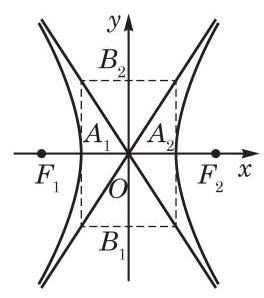
\includegraphics[max width=0.2\textwidth]{images/bo_d7fqvdc91nqc7381i9u0_65_1168_1668_264_298_0.jpg}
\end{center}
\hspace*{3em} 

图 2-3-6

双曲线与它的对称轴的交点叫做双曲线的顶点.

在方程 \circled{1} 中，令 \(y = 0\) ，得 \(x =  \pm  a\) ，所以 \({A}_{1}\left( {-a,0}\right)\) 、 \({A}_{2}\left( {a,0}\right)\) 是双曲线的两个顶点. 当 \(x = 0\) 时, \(y\) 没有实数解,所以双曲线与 \(y\) 轴没有交点,但我们也把点 \({B}_{1}\left( {0, - b}\right) \text{ 、 }{B}_{2}\left( {0,b}\right)\) 画在 \(y\) 轴上,如图 2-3-6 所示.

线段 \({A}_{1}{A}_{2}\) 和 \({B}_{1}{B}_{2}\) 分别在双曲线的两条对称轴上,我们把线段 \({A}_{1}{A}_{2}\) 叫做双曲线的实轴 (real axis),实轴的长是 \({2a}\) ; 线段 \({B}_{1}{B}_{2}\) 叫做双曲线的虚轴 (imaginary axis),虚轴的长是 \({2b}.a\) 和 \(b\) 分别叫做双曲线的实半轴长和虚半轴长. 双曲线的焦距为 \({2c}\) , 半焦距为 \(c\) ,且满足 \({c}^{2} = {a}^{2} + {b}^{2}\) . 显然,双曲线的两个焦点都在它的实轴所在直线上.

在方程 \(\frac{{x}^{2}}{{a}^{2}} - \frac{{y}^{2}}{{b}^{2}} = 1\) 中,如果 \(a = b\) ,那么这种双曲线的实轴和虚轴的长都等于 \({2a}\) . 我们把实轴和虚轴等长的双曲线叫做等轴双曲线.

\section*{(3)范围}

由方程 \circled{1} 可知 \(\frac{{x}^{2}}{{a}^{2}} - 1 = \frac{{y}^{2}}{{b}^{2}} \geq  0\) ,所以 \(\frac{{x}^{2}}{{a}^{2}} \geq  1\) ,也即 \(\left| x\right|  \geq  a\) , 且随着 \(\left| x\right|\) 不断增大, \(\left| y\right|\) 也相应地不断增大. 因此,双曲线 \(\frac{{x}^{2}}{{a}^{2}} - \frac{{y}^{2}}{{b}^{2}} = 1\) 在不等式 \(x \geq  a\) 和 \(x \leq   - a\) 所表示的区域内 (图 2-3-7), 且由两支组成: 一支双曲线在直线 \(x =  - a\) 的左侧,向左上、左下两方无限延伸; 另一支双曲线在直线 \(x = a\) 的右侧,向右上、 右下两方无限延伸.

\begin{center}
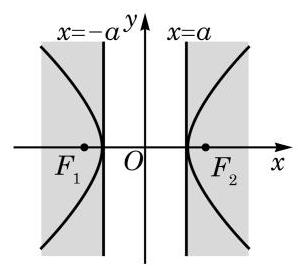
\includegraphics[max width=0.2\textwidth]{images/bo_d7fqvdc91nqc7381i9u0_66_198_687_298_268_0.jpg}
\end{center}
\hspace*{3em} 

图 2-3-7

\section*{(4) 渐近线}

双曲线 \(\frac{{x}^{2}}{{a}^{2}} - \frac{{y}^{2}}{{b}^{2}} = 1\) 在第一象限内部分的方程是

\[
y = \frac{b}{a}\sqrt{{x}^{2} - {a}^{2}}\left( {x > a}\right) .
\]

\begin{center}
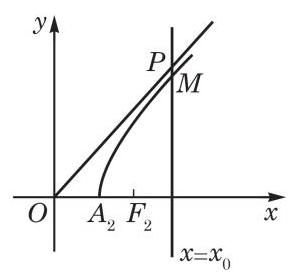
\includegraphics[max width=0.2\textwidth]{images/bo_d7fqvdc91nqc7381i9u0_66_199_1338_292_275_0.jpg}
\end{center}
\hspace*{3em} 

图 2-3-8

如图 2-3-8,设直线 \(x = {x}_{0}\left( {{x}_{0} > a > 0}\right)\) 与双曲线和射线 \(y = \; \frac{b}{a}x\left( {x > 0}\right)\) 分别交于点 \(M\left( {{x}_{0},{y}_{M}}\right) \text{ 、 }P\left( {{x}_{0},{y}_{P}}\right)\) ,可得

\[
{y}_{M} = \frac{b}{a}\sqrt{{x}_{0}^{2} - {a}^{2}} < \frac{b}{a}{x}_{0} = {y}_{P},
\]

即在第一象限内,双曲线总在射线 \(y = \frac{b}{a}x\left( {x > 0}\right)\) 的下方,且

\[
\left| {MP}\right|  = \frac{b}{a}{x}_{0} - \frac{b}{a}\sqrt{{x}_{0}^{2} - {a}^{2}}
\]

\[
= \frac{b}{a}\left( {{x}_{0} - \sqrt{{x}_{0}^{2} - {a}^{2}}}\right)
\]

\[
= \frac{ab}{{x}_{0} + \sqrt{{x}_{0}^{2} - {a}^{2}}}.
\]

因此,当 \({x}_{0}\) 逐渐增大时, \(\left| {MP}\right|\) 的值趋近于零.

这样,双曲线的右支向右上方无限延伸时,它总在直线 \(y = \frac{b}{a}x\) 的下方,与直线 \(y = \frac{b}{a}x\) 无限趋近,但永不相交.

根据对称性,双曲线 \(\frac{{x}^{2}}{{a}^{2}} - \frac{{y}^{2}}{{b}^{2}} = 1\) 和两条直线 \(y = \frac{b}{a}x,y =  - \frac{b}{a}x\) 在其他象限也有类似性质.

\HRule

这是双曲线与其他圆锥曲线不同的特有性质.

\HRule

\begin{center}
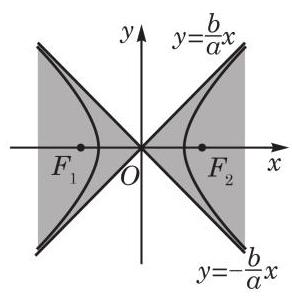
\includegraphics[max width=0.2\textwidth]{images/bo_d7fqvdc91nqc7381i9u0_67_1155_707_292_298_0.jpg}
\end{center}
\hspace*{3em} 

图 2-3-9

我们把直线 \(y = \frac{b}{a}x\) 和 \(y =  - \frac{b}{a}x\) 叫做双曲线 \(\frac{{x}^{2}}{{a}^{2}} - \frac{{y}^{2}}{{b}^{2}} = 1\) 的渐近线 (asymptote). 可以证明, 双曲线位于以两条渐近线为边界的左、右平面区域内(图 2-3-9).

\section*{(5) 离心率}

双曲线的焦距与实轴长的比 \(e = \frac{c}{a}\) ,叫做双曲线的离心率.

因为 \(c > a > 0\) ,所以双曲线的离心率 \(e > 1\) .

由等式 \({c}^{2} - {a}^{2} = {b}^{2}\) ,可得

\[
\frac{b}{a} = \frac{\sqrt{{c}^{2} - {a}^{2}}}{a} = \sqrt{{\left( \frac{c}{a}\right) }^{2} - 1} = \sqrt{{e}^{2} - 1}.
\]

因此,离心率 \(e\) 越大, \(\frac{b}{a}\) 也越大,即渐近线 \(y =  \pm  \frac{b}{a}x\) 的斜率的绝对值越大, 这时双曲线的形状就从扁狭逐渐变得开阔. 这说明, 双曲线的离心率越大, 它的开口就越开阔; 反之, 离心率越小,双曲线的开口就越狭窄.

例 4 求双曲线 \({16}{x}^{2} - 9{y}^{2} = {144}\) 的顶点坐标、焦点坐标、离心率与渐近线方程.

解 把给定的双曲线的方程化成标准方程

\[
\frac{{x}^{2}}{9} - \frac{{y}^{2}}{16} = 1
\]

因此实半轴的长 \(a = 3\) ,虚半轴的长 \(b = 4\) . 于是

\[
c = \sqrt{{a}^{2} + {b}^{2}} = 5,
\]

从而双曲线的两个顶点的坐标分别是 \(\left( {-3,0}\right) \text{ 、 }\left( {3,0}\right)\) ,两个焦点的坐标分别是 \(\left( {-5,0}\right) \text{ 、 }\left( {5,0}\right)\) ,离心率为 \(e = \frac{c}{a} = \frac{5}{3}\) ,两条渐近线的方程是 \(y = \frac{4}{3}x\) 和 \(y =  - \frac{4}{3}x\) .

\section*{练习 2.3(2)}

1. 分别写出下列双曲线的实半轴长、虚半轴长、离心率、焦点坐标、顶点坐标和渐近线方程:

(1) \(9{x}^{2} - {16}{y}^{2} = {144}\) ；

(2) \(\frac{{y}^{2}}{4} - \frac{{x}^{2}}{3} = 1\) .

2. 在下列双曲线中,以 \(y =  \pm  \frac{1}{2}x\) 为渐近线的是 ( )

A. \(\frac{{x}^{2}}{16} - \frac{{y}^{2}}{4} = 1\) ; B. \(\frac{{x}^{2}}{4} - \frac{{y}^{2}}{16} = 1\) ; C. \(\frac{{x}^{2}}{2} - {y}^{2} = 1\) ; D. \({x}^{2} - \frac{{y}^{2}}{2} = 1\) .

3. 判断双曲线 \(\frac{{x}^{2}}{4} - \frac{{y}^{2}}{5} = 1\) 与双曲线 \(\frac{{y}^{2}}{5} - \frac{{x}^{2}}{4} = 1\) 的四个焦点是否共圆.

例 5 已知双曲线过点 \(P\left( {4,3}\right)\) ,它的一条渐近线的方程为 \(y = \frac{1}{2}x\) . 求双曲线的标准方程.

\begin{center}
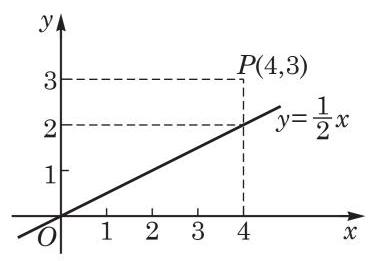
\includegraphics[max width=0.3\textwidth]{images/bo_d7fqvdc91nqc7381i9u0_68_160_1091_369_261_0.jpg}
\end{center}
\hspace*{3em} 

图 2-3-10

解 因为双曲线的一条渐近线方程为 \(y = \frac{1}{2}x\) ,当 \(x = 4\) 时, 渐近线上对应点的纵坐标为 \(y = \frac{1}{2} \times  4 = 2\) ,小于点 \(P\) 的纵坐标 3 (图 2-3-10),所以双曲线的焦点在 \(y\) 轴上. 设双曲线的标准方程为

\[
\frac{{y}^{2}}{{a}^{2}} - \frac{{x}^{2}}{{b}^{2}} = 1\left( {a > 0,b > 0}\right) .
\]

由 \(y = \frac{1}{2}x\) ,可知 \(\frac{a}{b} = \frac{1}{2}\) . 若令 \(a = k\) ,则 \(b = {2k}\) .

?

又因为点 \(P\left( {4,3}\right)\) 在双曲线上,所以

\[
\frac{9}{{k}^{2}} - \frac{16}{4{k}^{2}} = 1
\]

\HRule

如果双曲线的渐近线方程是 \(y =  \pm  \frac{m}{n}x \; \left( {m > 0,n > 0}\right)\) ,即 \({mx} \pm  {ny} = 0\) ,那么双曲线的方程应具有什么形式?

\HRule

解得 \({k}^{2} = 5\) .

因此,所求双曲线的标准方程为 \(\frac{{y}^{2}}{5} - \frac{{x}^{2}}{20} = 1\) .

例 6 设直线与双曲线的方程分别为 \(y = {kx}\) 和 \({x}^{2} - {y}^{2} =\) 1,当实数 \(k\) 取何值时,直线与双曲线分别有两个公共点? 有一个公共点? 没有公共点?

解 将直线方程 \(y = {kx}\) 代入双曲线方程 \({x}^{2} - {y}^{2} = 1\) ,得

\[
\left( {1 - {k}^{2}}\right) {x}^{2} = 1.
\]
  \circled{1} 

当 \(1 - {k}^{2} > 0\) ,即 \(\left| k\right|  < 1\) 时,方程 \circled{1} 有两个不同的实根 \(x = \; \pm  \sqrt{\frac{1}{1 - {k}^{2}}}\) ,从而直线与双曲线有两个公共点; 当 \(1 - {k}^{2} \leq  0\) ,即 \(\left| k\right|  \geq  1\) 时,方程 \circled{1} 无实根,从而直线与双曲线没有公共点; 直线与双曲线只有一个公共点的情况不存在.

\begin{center}
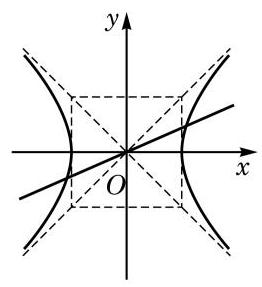
\includegraphics[max width=0.2\textwidth]{images/bo_d7fqvdc91nqc7381i9u0_69_1170_340_262_287_0.jpg}
\end{center}
\hspace*{3em} 

图 2-3-11

例 6 的结果从图像上(图 2-3-11)看也是显然的，因为此双曲线夹在两条渐近线 \(y =  \pm  x\) 之间的左右平面区域内,所以只有当直线也经过这个区域时, 它与双曲线才有公共点.

例 7 双曲线型自然冷却通风塔的外形是由双曲线的一部分绕其虚轴所在的直线旋转一周所形成的曲面, 如图 2-3-12 所示. 已知它的最小半径为 \({12}\mathrm{\;m}\) ,上口半径为 \({13}\mathrm{\;m}\) ,下口半径为 \({25}\mathrm{\;m}\) ,高为 \({55}\mathrm{\;m}\) . 建立适当的平面直角坐标系,求此双曲线的方程. (结果精确到 \({0.1}\mathrm{\;m}\) )

\begin{center}
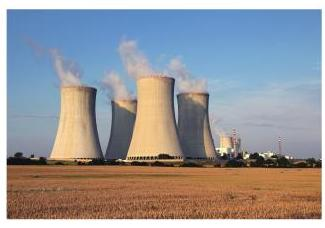
\includegraphics[max width=0.2\textwidth]{images/bo_d7fqvdc91nqc7381i9u0_69_1139_755_325_228_0.jpg}
\end{center}
\hspace*{3em} 

\begin{center}
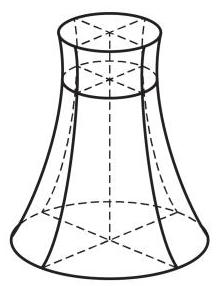
\includegraphics[max width=0.2\textwidth]{images/bo_d7fqvdc91nqc7381i9u0_69_324_1090_216_286_0.jpg}
\end{center}
\hspace*{3em} 

图 2-3-12

\begin{center}
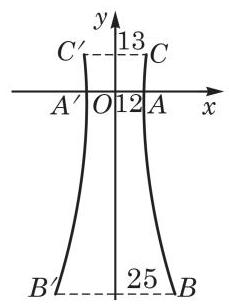
\includegraphics[max width=0.2\textwidth]{images/bo_d7fqvdc91nqc7381i9u0_69_715_1083_229_307_0.jpg}
\end{center}
\hspace*{3em} 

图 2-3-13

解 图 2-3-13 是通风塔过中轴的剖面. 以剖面最窄处的水平线为 \(x\) 轴,则 \(x\) 轴与双曲线的交点 \({A}^{\prime }\) 与 \(A\) 是双曲线的顶点; 又以通风塔的中轴为 \(y\) 轴. 在这样的平面直角坐标系中,设双曲线的标准方程是

\[
\frac{{x}^{2}}{{a}^{2}} - \frac{{y}^{2}}{{b}^{2}} = 1\left( {a > 0,b > 0}\right) .
\]

点 \(B\text{ 、 }C\) 的坐标可分别设为 \(\left( {{25},{y}_{1}}\right) \text{ 、 }\left( {{13},{y}_{2}}\right)\) ,其中 \({y}_{1} < 0\) , \({y}_{2} > 0\) . 又因为塔高为 \({55}\mathrm{\;m}\) ,所以 \({y}_{2} - {y}_{1} = {55}\) .

由 \(A{A}^{\prime }\) 是双曲线的实轴,得 \(a = {12}\) .

因为点 \(B\text{ 、 }C\) 在双曲线上,所以

\[
\frac{{25}^{2}}{{12}^{2}} - \frac{{y}_{1}^{2}}{{b}^{2}} = 1,\frac{{13}^{2}}{{12}^{2}} - \frac{{y}_{2}^{2}}{{b}^{2}} = 1.
\]

解得

\[
{y}_{1} =  - \frac{\sqrt{481}b}{12},{y}_{2} = \frac{5b}{12}.
\]

代入 \({y}_{2} - {y}_{1} = {55}\) ,得

\[
\frac{5b}{12} + \frac{\sqrt{481}b}{12} = {55}
\]

解得 \(b \approx  {24.5}\) .

因此，所求双曲线的方程为

\[
\frac{{x}^{2}}{{12}^{2}} - \frac{{y}^{2}}{{24.5}^{2}} = 1.
\]

\section*{练习 2.3(3)}

1. 求适合下列条件的双曲线的标准方程:

(1)顶点在 \(x\) 轴上，两顶点间的距离是 10，且经过点 \(\left( {{10},3}\right)\) ；

(2)一个焦点的坐标为 \(\left( {5,0}\right)\) ，一条渐近线方程为 \({3x} - {4y} = 0\) .

2. 给定一对直线 \(y =  \pm  \frac{b}{a}x\left( {a > 0,b > 0}\right)\) ,写出所有以这对直线为渐近线的、实轴在 \(x\) 轴上的双曲线的方程.

3. 联系双曲线 \(\frac{{x}^{2}}{{a}^{2}} - \frac{{y}^{2}}{{b}^{2}} = 1\left( {a > 0,b > 0}\right)\) 的性质,讨论并叙述双曲线 \(\frac{{y}^{2}}{{a}^{2}} - \frac{{x}^{2}}{{b}^{2}} = 1(a > 0\) , \(b > 0\) )的性质. (不要求推理过程)

\section*{习题 2.3}

\section*{A 组}

1. 双曲线 \(\frac{{x}^{2}}{64} - \frac{{y}^{2}}{36} = 1\) 上一点 \(P\) 到焦点 \({F}_{1}\) 的距离等于 6,求点 \(P\) 到另一焦点 \({F}_{2}\) 的距离.

2. 已知双曲线以坐标轴为对称轴, 两个顶点间的距离为 2 , 焦点到渐近线的距离为 \(\sqrt{2}\) . 求该双曲线的方程.

3. 如果双曲线关于原点对称, 它的焦点在坐标轴上, 实轴的长为 8 , 焦距为 10 . 写出此双曲线的方程.

4. 如果方程 \(\frac{{x}^{2}}{m + 2} - \frac{{y}^{2}}{m + 1} = 1\) 表示焦点在 \(y\) 轴上的双曲线,求实数 \(m\) 的取值范围.

5. 已知双曲线经过点 \(\left( {1,1}\right)\) ,其渐近线方程为 \(y =  \pm  \sqrt{2}x\) . 求此双曲线的方程.

\section*{B 组}

1. 已知双曲线的中心在原点,焦点在 \(y\) 轴上,并且双曲线上两点 \({P}_{1}\text{ 、 }{P}_{2}\) 的坐标分别为 \(\left( {3, - 4\sqrt{2}}\right) \text{ 、 }\left( {\frac{9}{4},5}\right)\) . 求该双曲线的方程.

2. 已知离心率为 \(\frac{5}{3}\) 的双曲线与椭圆 \(\frac{{x}^{2}}{40} + \frac{{y}^{2}}{15} = 1\) 有公共焦点,求此双曲线的方程.

3. \(A\text{ 、 }B\text{ 、 }C\) 是我方三个炮兵阵地. \(A\) 地在 \(B\) 地的正东,相距 \(6\mathrm{\;{km}};C\) 地在 \(B\) 地的北偏西 \({30}^{ \circ  }\) ,相距 \(4\mathrm{\;{km}}.P\) 为敌方炮兵阵地. 某时刻 \(A\) 地发现 \(P\) 地某种信号, \({12}\mathrm{\;s}\) 后 \(B\text{ 、 }C\) 两地才同时发现这种信号 (该信号的传播速度为 \({0.333}\mathrm{\;{km}}/\mathrm{s}\) ). 若从 \(A\) 地炮击 \(P\) 地,求准确炮击的方位角. (结果精确到 \({1}^{ \circ  }\) )

\section*{2.4 抛物线}

\section*{1 抛物线的标准方程}

抛物线是一种常见的曲线, 例如喷泉中喷出的水珠、投出的篮球所经过的轨迹都是抛物线. 抛物线的用途很广泛, 在太阳灶、探照灯、雷达天线、卫星天线、射电望远镜、工程建筑等工程技术中都有它的身影, 体现了抛物线在光学、力学等方面的独有特性.

\begin{center}
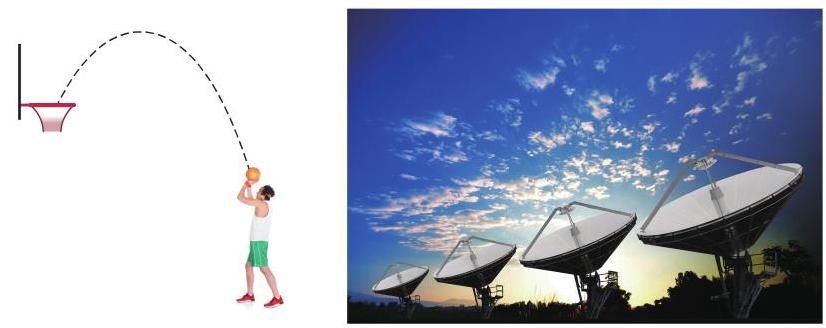
\includegraphics[max width=0.7\textwidth]{images/bo_d7fqvdc91nqc7381i9u0_72_610_1057_826_328_0.jpg}
\end{center}
\hspace*{3em} 

与椭圆、双曲线一样, 我们也通过操作先画出一段抛物线, 然后建立平面直角坐标系推导抛物线方程. 如图 2-4-1, 将一把直尺在一个平面上固定不动. 另取一块三角板，设直角顶点为 \(C\) ，并在它的一条直角边上取定点 \(A\) . 再取一条细线使它的长度正好等于 \({AC}\) 的长. 将这条细线的一端固定在三角板的点 \(A\) ,另一端固定在同一平面上的点 \(F\) . 用一支铅笔靠着细线将它绷紧，当三角板的另一条直角边靠着直尺滑动时,铅笔尖 \(P\) 画出了一段曲线. 观察这段曲线的生成过程可以发现,如果把直尺看作一条定直线 \(l\) ,那么动点 \(P\) 到直线 \(l\) 的距离始终等于它到定点 \(F\) 的距离.

\begin{center}
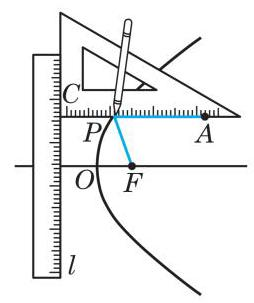
\includegraphics[max width=0.2\textwidth]{images/bo_d7fqvdc91nqc7381i9u0_72_218_1418_254_303_0.jpg}
\end{center}
\hspace*{3em} 

图 2-4-1

一般地,平面上到一个定点 \(F\) 和到一条定直线 \(l\) ( \(F\) 不在 \(l\) 上)距离相等的点的轨迹叫做抛物线 (parabola),点 \(F\) 叫做抛物线的焦点,定直线 \(l\) 叫做抛物线的准线 (directrix). 过点 \(F\) 作准线 \(l\) 的垂线,设垂足为 \(K\) ,则线段 \({KF}\) 的中点称为此抛物线的顶 ? 点. 因为这一点到点 \(F\) 和到直线 \(l\) 的距离相等,所以这是抛物线上的一点.

\HRule

为什么需加条件 “ \(F\) 不在 \(l\) 上”?

\HRule

下面根据抛物线的定义来求它的方程.

\begin{center}
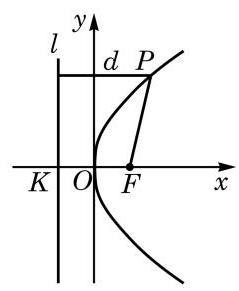
\includegraphics[max width=0.2\textwidth]{images/bo_d7fqvdc91nqc7381i9u0_73_1178_400_239_291_0.jpg}
\end{center}
\hspace*{3em} 

图 2-4-2

如图 2-4-2,取抛物线的顶点为原点 \(O\) ,以向量 \(\overrightarrow{KF}\) 的方向为 \(x\) 轴的正方向,建立平面直角坐标系.

设焦点到准线的距离 \(\left| {KF}\right|  = p\left( {p > 0}\right)\) ,则焦点 \(F\) 的坐标是 \(\left( {\frac{p}{2},0}\right)\) ,准线 \(l\) 的方程为 \(x =  - \frac{p}{2}\) .

设 \(P\left( {x,y}\right)\) 是抛物线上任意一点,点 \(P\) 到 \(l\) 的距离为 \(d\) ,则

\[
\left| {PF}\right|  = \sqrt{{\left( x - \frac{p}{2}\right) }^{2} + {y}^{2}},d = \left| {x + \frac{p}{2}}\right| .
\]

由抛物线定义知 \(\left| {PF}\right|  = d\) ,于是有

\[
\sqrt{{\left( x - \frac{p}{2}\right) }^{2} + {y}^{2}} = \left| {x + \frac{p}{2}}\right| .
\]

\HRule

这里, 还可以怎样建立平面直角坐标系? 相应的抛物线方程又具有怎样的形式?

\HRule

将上式两边平方, 并化简, 得

\[
{y}^{2} = {2px}\left( {p > 0}\right) .
\]

从这个推导过程可以知道,抛物线上任意一点 \(M\) 的坐标 \(\left( {x,y}\right)\) 都是上述方程的解. 反过来, 可以证明以上述方程的解为坐标的点, 都在这条抛物线上 (只需将上述推理过程反过来推演即可).

\HRule

我们学过二次函数 \(y = a{x}^{2} + {bx} + c(a \neq\) 0)的图像，可以看出， 当 \(b = c = 0\) 时，此图像是一个具有方程 \({x}^{2} = {2py}\left( {\text{ 此时 }p = \frac{1}{2a}}\right)\) 的抛物线. 当 \(b\text{ 、 }c\) 不全为零时, 二次函数的图像是这个抛物线的平移.

\HRule

形如 \({y}^{2} = {2px}\) ( \(p > 0\) )的方程叫做抛物线的标准方程,它所表示的抛物线的顶点置于坐标原点,且具有焦点 \(F\left( {\frac{p}{2},0}\right)\) 和准线 \(l : x =  - \frac{p}{2}\) . 我们还注意到,这条抛物线上任何一点的横坐标 \(x \geq  0\) , 所以抛物线位于 \(y\) 轴及其右侧; 当 \(x\) 增大时,抛物线上相应点的纵坐标 \(y\) 的绝对值也随着增大. 可见,此抛物线从顶点出发的上下两部分随着 \(x\) 的增大,在 \(x\) 轴的正方向 (即坐标系的右方) 形成了不再封闭的开口(我们形象地称此抛物线的“开口向右”). Q

仿照上述过程, 如果将抛物线的顶点仍置于坐标原点, 但将焦点分别置于 \(x\) 轴的负半轴、 \(y\) 轴的正半轴和负半轴,就可以相应地得到抛物线的另外三种标准方程: \({y}^{2} =  - {2px},{x}^{2} = {2py}\) 与 \({x}^{2} =  - {2py}\) . 其中,后两种形式稍作变形就是我们所熟知的二次函数的表达式.

例 1 求顶点在坐标原点, 焦点在坐标轴上且经过点 \(M\left( {-2, - 4}\right)\) 的抛物线的方程.

\begin{center}
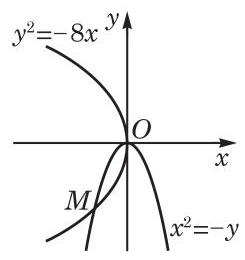
\includegraphics[max width=0.2\textwidth]{images/bo_d7fqvdc91nqc7381i9u0_74_224_372_245_260_0.jpg}
\end{center}
\hspace*{3em} 

图 2-4-3

解 由于抛物线的顶点在坐标原点, 焦点在坐标轴上, 因此抛物线的方程是上述四种标准方程之一.

若抛物线的焦点在 \(x\) 轴上,由于它过第三象限的点 \(M\left( {-2, - 4}\right)\) , 可知此抛物线开口向左 (图 2-4-3), 因此可设其方程为

\[
{y}^{2} =  - {2px}\left( {p > 0}\right) .
\]

把点 \(M\) 的坐标代入,得到

\[
{\left( -4\right) }^{2} =  - {2p} \cdot  \left( {-2}\right) .
\]

解得 \(p = 4\) . 从而抛物线的方程为 \({y}^{2} =  - {8x}\) .

若抛物线的焦点在 \(y\) 轴上,由于它过第三象限的点 \(M\left( {-2, - 4}\right)\) , 可知此抛物线开口向下(图 2-4-3)，因此可设其方程为

\[
{x}^{2} =  - {2py}\left( {p > 0}\right) \text{ . }
\]

把点 \(M\) 的坐标代入,得到

\[
{\left( -2\right) }^{2} =  - {2p} \cdot  \left( {-4}\right) .
\]

解得 \(p = \frac{1}{2}\) . 从而抛物线的方程为 \({x}^{2} =  - y\) .

因此,所求抛物线的方程为 \({y}^{2} =  - {8x}\) 或 \({x}^{2} =  - y\) .

例 2 证明: 以抛物线 \({y}^{2} = {2px}\) 的任一过焦点的弦为直径的圆与抛物线的准线相切.

\begin{center}
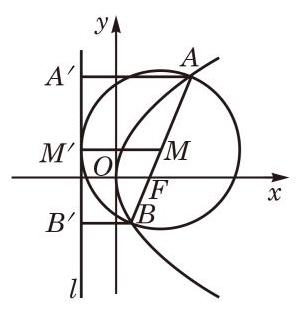
\includegraphics[max width=0.2\textwidth]{images/bo_d7fqvdc91nqc7381i9u0_74_201_1442_297_309_0.jpg}
\end{center}
\hspace*{3em} 

图 2-4-4

证明 如图 2-4-4,设 \({AB}\) 是此抛物线过焦点 \(F\) 的一条弦, 取 \({AB}\) 的中点 \(M\) ,设点 \(A\text{ 、 }B\text{ 、 }M\) 在抛物线的准线 \(l\) 上的射影依次是点 \({A}^{\prime }\text{ 、 }{B}^{\prime }\text{ 、 }{M}^{\prime }\) ,则 \(M{M}^{\prime }\) 是直角梯形 \(A{A}^{\prime }{B}^{\prime }B\) 的中位线.

因为点 \(A\text{ 、 }B\) 在抛物线上,所以

\[
\left| {A{A}^{\prime }}\right|  = \left| {AF}\right| ,\left| {B{B}^{\prime }}\right|  = \left| {BF}\right| .
\]

于是

\[
\left| {M{M}^{\prime }}\right|  = \frac{1}{2}\left( {\left| {A{A}^{\prime }}\right|  + \left| {B{B}^{\prime }}\right| }\right)  = \frac{1}{2}\left( {\left| {AF}\right|  + \left| {BF}\right| }\right)  = \frac{1}{2}\left| {AB}\right| .
\]

即点 \(M\) 到准线的距离等于圆的半径.

由此可见,以 \({AB}\) 为直径的圆与准线 \(l\) 相切.

\section*{练习 2.4(1)}

1. 填写下表:

\begin{center}
\adjustbox{max width=\textwidth}{
\begin{tabular}{|c|c|c|c|c|}
\hline
图示 & 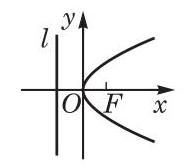
\includegraphics[max width=0.2\textwidth]{images/bo_d7fqvdc91nqc7381i9u0_75_387_459_188_168_0.jpg} & 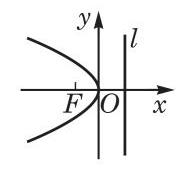
\includegraphics[max width=0.2\textwidth]{images/bo_d7fqvdc91nqc7381i9u0_75_664_459_188_170_0.jpg} & \phantom{X} & \phantom{X} \\
\cline{1-5}
标准方程 & \({y}^{2} = {2px}\left( {p > 0}\right)\) & \phantom{X} & \({x}^{2} = {2py}\left( {p > 0}\right)\) & \phantom{X} \\
\cline{1-5}
焦点坐标 & \(\left( {\frac{p}{2},0}\right)\) & \phantom{X} & \phantom{X} & \(\left( {0, - \frac{p}{2}}\right)\) \\
\cline{1-5}
准线方程 & \(x =  - \frac{p}{2}\) & \phantom{X} & \phantom{X} & \(y = \frac{p}{2}\) \\
\cline{1-5}
\hline
\end{tabular}
}
\end{center}

2. 分别写出满足下列条件的抛物线的标准方程:

(1)焦点是 \(F\left( {-2,0}\right)\) ；

(2)准线方程是 \(y = 1\) .

3. 求抛物线 \({y}^{2} = {4x}\) 上到焦点的距离等于 9 的点的坐标.

\section*{2 抛物线的性质}

下面，我们以顶点在原点、焦点在 \(x\) 轴正半轴上的抛物线为例, 讨论抛物线的性质. 此时抛物线的标准方程为:

\[
{y}^{2} = {2px}\left( {p > 0}\right) .
\]

\section*{(1) 对称性}

因为抛物线上任意一点 \(M\left( {x,y}\right)\) 关于 \(x\) 轴的对称点 \({M}^{\prime }\left( {x, - y}\right)\) 也满足方程,所以抛物线 \({y}^{2} = {2px}\) 关于 \(x\) 轴对称. 抛物线有且只有一条对称轴. 对称轴与抛物线的交点就是抛物线的顶点.

\section*{(2)范围}

因为 \(p > 0\) ,由方程 \({y}^{2} = {2px}\) 可知 \(x \geq  0\) ,抛物线的开口向右. 除原点外,这条抛物线上的点都在 \(y\) 轴的右侧,且当 \(x\) 无限增大时, \(\left| y\right|\) 也无限增大. 这说明此抛物线向右上方和右下方无限延伸.

从抛物线方程可知,对于同一个 \(x\) 值,当 \(p\) 越大, \(\left| y\right|\) 就越大. 这说明 \(p\) 越大,抛物线的开口就越大.

例 3 过抛物线 \({y}^{2} = {4x}\) 的焦点且斜率为 2 的直线与抛物线相交于 \(A\text{ 、 }B\) 两点,求线段 \({AB}\) 的长.

解 由题意可知,抛物线的焦点为 \(F\left( {1,0}\right)\) ,则直线的方程为

\[
y = 2\left( {x - 1}\right) .
\]
  \circled{1} 

将方程 \circled{1} 代入抛物线方程 \({y}^{2} = {4x}\) ，并化简得

\[
{x}^{2} - {3x} + 1 = 0.
\]

设两个交点 \(A\text{ 、 }B\) 的坐标分别为 \(\left( {{x}_{1},{y}_{1}}\right) \text{ 、 }\left( {{x}_{2},{y}_{2}}\right)\) ,则有 \({x}_{1} + {x}_{2} = 3.\)

例 4 求过定点 \(M\left( {0,1}\right)\) 且与抛物线 \({y}^{2} = {2x}\) 只有一个公共点的直线的方程.

\begin{center}
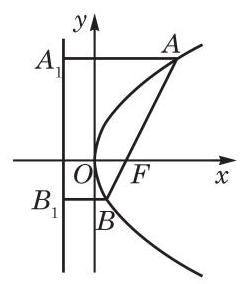
\includegraphics[max width=0.2\textwidth]{images/bo_d7fqvdc91nqc7381i9u0_76_226_1069_242_284_0.jpg}
\end{center}
\hspace*{3em} 

图 2-4-5

由抛物线定义可知, \(\left| {AF}\right| \text{ 、 }\left| {BF}\right|\) 分别等于点 \(A\text{ 、 }B\) 到准线 \(x =  - 1\) 的距离 \(\left| {A{A}_{1}}\right| \text{ 、 }\left| {B{B}_{1}}\right|\) ,如图 2-4-5 所示.

又因为 \(\left| {A{A}_{1}}\right|  = {x}_{1} + 1,\left| {B{B}_{1}}\right|  = {x}_{2} + 1\) ,所以

\[
\left| {AB}\right|  = \left| {AF}\right|  + \left| {BF}\right|  = \left| {A{A}_{1}}\right|  + \left| {B{B}_{1}}\right|  = {x}_{1} + {x}_{2} + 2 = 5.
\]

解 先考虑过点 \(M\left( {0,1}\right)\) 且不垂直于 \(x\) 轴的直线,可设其方程为 \(y = {kx} + 1\) .

由方程组 \(\left\{  \begin{array}{l} y = {kx} + 1, \\  {y}^{2} = {2x}, \end{array}\right.\) 得

\[
{k}^{2}{x}^{2} + 2\left( {k - 1}\right) x + 1 = 0.
\]
  \circled{1} 

当 \(k = 0\) 时,方程 \circled{1} 为一元一次方程,其解为 \(x = \frac{1}{2}\) ,此时直线 \(y = 1\) 与抛物线只有一个公共点 \(P\left( {\frac{1}{2},1}\right)\) .

当 \(k \neq  0\) 时,方程 \circled{1} 为一元二次方程,它只有一个解的充要条件是其判别式 \(\Delta  = 4{\left( k - 1\right) }^{2} - 4{k}^{2} = 0\) ,解得 \(k = \frac{1}{2}\) . 由此得到直线 \(y = \frac{1}{2}x + 1\) 与抛物线也只有一个公共点. ?

\HRule

例 4 中, 判别式为零是直线与抛物线仅有一个公共点的什么条件?

\HRule

\begin{center}
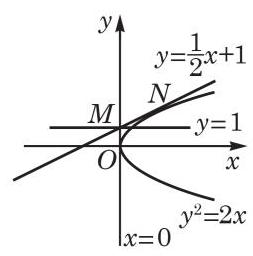
\includegraphics[max width=0.2\textwidth]{images/bo_d7fqvdc91nqc7381i9u0_77_1170_238_253_256_0.jpg}
\end{center}
\hspace*{3em} 

图 2-4-6

此外,过点 \(M\left( {0,1}\right)\) 且垂直于 \(x\) 轴的直线 \(x = 0\) 也满足题意 (图 2-4-6).

因此,所求直线的方程为 \(y = 1\) 或 \(y = \frac{1}{2}x + 1\) 或 \(x = 0\) .

在前面学习圆和椭圆时, 我们曾经介绍过圆和椭圆的切线, 可以发现, 当直线与圆或椭圆有且仅有一个公共点时, 直线与圆或椭圆相切. 这仅仅是对圆或椭圆而言的情况. 由例 4 知, 在抛物线的情况下没有这样的结论. 例如, 当一条直线平行于一条抛物线的对称轴时 (如例 4 中的直线 \(y = 1\) ),这条直线与这条抛物线有且只有一个公共点, 但它不是抛物线的切线 (切线的确切含义见选择性必修课程 5.1 节).

例 5 如图 2-4-7, 汽车前灯反射镜与轴截面的交线是抛物线的一部分，灯泡位于抛物线的焦点处. 已知灯口直径是 \({24}\mathrm{\;{cm}}\) ， 灯深 10 cm，求灯泡与反射镜顶点的距离.

\HRule

抛物线具有如下的光学性质:所有从抛物线焦点发出的光线经过抛物线反射后都与这条抛物线的对称轴平行或重合. 制作探照灯、汽车远光灯时正是依据这个原理，把光源放在抛物线的焦点处，使得光线经过抛物面的反射后都变成平行光束, 照得又亮又远.

\HRule

\begin{center}
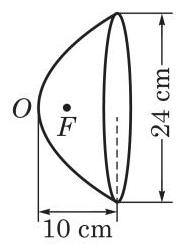
\includegraphics[max width=0.2\textwidth]{images/bo_d7fqvdc91nqc7381i9u0_77_351_1068_181_244_0.jpg}
\end{center}
\hspace*{3em} 

图 2-4-7

\begin{center}
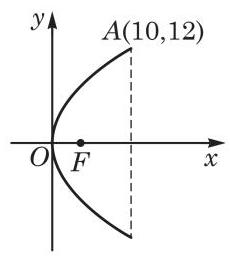
\includegraphics[max width=0.2\textwidth]{images/bo_d7fqvdc91nqc7381i9u0_77_668_1057_230_258_0.jpg}
\end{center}
\hspace*{3em} 

图 2-4-8

解 以抛物线的对称轴为 \(x\) 轴,抛物线的顶点为原点,建立平面直角坐标系, 如图 2-4-8 所示.

由题意,得点 \(A\) 的坐标为 \(\left( {{10},{12}}\right)\) .

设抛物线的方程为

\[
{y}^{2} = {2px}\left( {p > 0}\right) .
\]

因为点 \(A\) 在抛物线上,所以

\[
{12}^{2} = {2p} \cdot  {10},
\]

解得 \(p = {7.2}\) . 因此,抛物线焦点 \(F\) 的坐标为 \(\left( {{3.6},0}\right)\) .

所以，灯泡与反射镜顶点的距离为 \({3.6}\mathrm{\;{cm}}\) .

\section*{练习 2.4(2)}

1. 过点 \(P\left( {2,4}\right)\) 且与抛物线 \({y}^{2} = {8x}\) 有且只有一个公共点的直线有 ( )

A. 1 条; B. 2 条; C. 3 条; D. 4 条.

圆锥曲线

2. 求抛物线 \({y}^{2} = {4x}\) 上的点到直线 \({4x} + {3y} + 7 = 0\) 的最短距离.

3. 由抛物线的标准方程知,函数 \(y = \sqrt{x}\) 的图像是某条抛物线的一部分. 求这条抛物线的焦点坐标和准线方程.

\section*{习题 2.4}

\section*{A 组}

1. 求抛物线 \({y}^{2} = {ax}\left( {a \neq  0}\right)\) 的焦点坐标和准线方程.

2. 若抛物线 \({y}^{2} = {2x}\) 上的 \(A\) 、 \(B\) 两点到焦点 \(F\) 的距离之和是 5,求线段 \({AB}\) 的中点的横坐标.

3. 求以坐标原点为顶点,以 \(y\) 轴为对称轴,并经过点 \(P\left( {-6, - 3}\right)\) 的抛物线的标准方程.

4. 已知直线 \(y = {kx} - 4\) 与抛物线 \({y}^{2} = {8x}\) 有且只有一个公共点，求实数 \(k\) 的值.

5. 已知一隧道的顶部是抛物拱形,拱高是 \(5\mathrm{\;m}\) ,跨度为 \({10}\mathrm{\;m}\) . 建立适当的平面直角坐标系, 求此拱形所在的抛物线方程.

\section*{B 组}

1. 已知动点 \(P\) 与定点 \(\left( {1,0}\right)\) 的距离比点 \(P\) 到 \(y\) 轴的距离大 1,求动点 \(P\) 的轨迹方程.

2. 过抛物线 \({y}^{2} = {2px}\left( {p > 0}\right)\) 焦点的一条直线与抛物线相交于两个不同的点,求证: 这两个点的纵坐标 \({y}_{1}\text{ 、 }{y}_{2}\) 满足 \({y}_{1}{y}_{2} =  - {p}^{2}\) .

3. 过抛物线 \({y}^{2} = {2px}\left( {p > 0}\right)\) 的焦点且倾斜角为 \(\alpha\) 的直线 \(l\) 与抛物线交于 \(A\text{ 、 }B\) 两点， 求证: \(\left| {AB}\right|  = \frac{2p}{{\sin }^{2}\alpha }\) .

\section*{课后阅读}

\section*{章名“圆锥曲线”释义}

本章的前面几节分别学习了圆、椭圆、双曲线和抛物线, 但这一章的章名却叫“圆锥曲线”, 这是为什么呢? 这些曲线与圆锥有什么关系呢? 下面就来探讨这些问题.

如图 2-4-9, 我们取两个相同的圆锥, 把其中一个倒置后组成一个共顶点、共轴的旋转体, 想象这个旋转体可上下无限延伸. 设圆锥的旋转轴与母线所成的角为 \(\alpha\) ,用一不过圆锥顶点的平面截这个圆锥,设这个平面与圆锥旋转轴所成的角为 \(\theta\) ,则平面与圆锥的侧面相截得到的平面曲线有以下几种情况:

\HRule

这个旋转体也可以看作是由两条相交直线绕其角平分线旋转而成.

\HRule

(1)当 \(\alpha  < \theta  \leq  \frac{\pi }{2}\) 时，平面与圆锥的侧面相截所得的是一个椭圆，如图 2-4-9(1)所示； 特别地,当 \(\theta  = \frac{\pi }{2}\) 时,得到的是一个圆.

(2)当 \(\alpha  = \theta\) ，即平面与圆锥的一条母线平行时，所截得的是一条抛物线，如图 2-4-9(2) 所示.

(3)当 \(0 \leq  \theta  < \alpha\) ，且这个平面不经过圆锥的顶点时，所截得的是一条双曲线，如图 2-4-9(3)所示.

\begin{center}
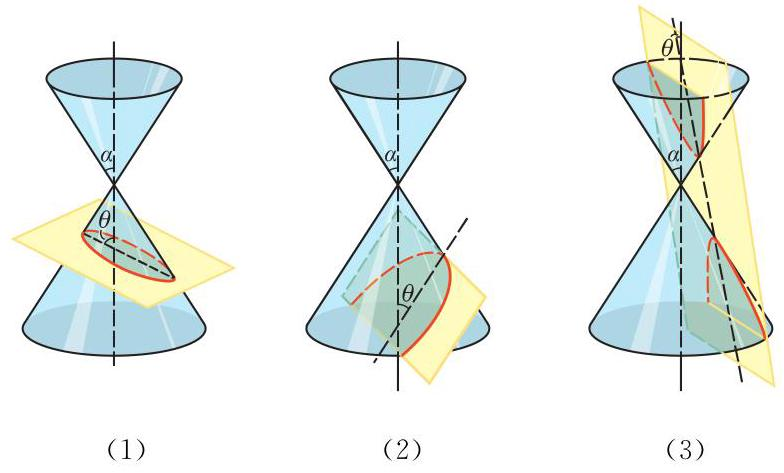
\includegraphics[max width=0.6\textwidth]{images/bo_d7fqvdc91nqc7381i9u0_79_402_950_784_473_0.jpg}
\end{center}
\hspace*{3em} 

图 2-4-9

可见, 椭圆 (包括圆)、抛物线、双曲线都可以看作是由不同的平面截同一个圆锥得到的, 所以它们统称为圆锥曲线 (conic sections). 这是本章章名的由来.

\section*{*2.5 曲线与方程}

\section*{1 求轨迹的方程}

在本章 2.1 节中我们给出了曲线方程的定义. 根据此定义, 要确认一个二元方程 \(F\left( {x,y}\right)  = 0\) 是一条平面曲线 \(C\) 的方程,必须验证如下两个条件都满足:

 \circled{1}  曲线 \(C\) 上的点的坐标都是方程 \(F\left( {x,y}\right)  = 0\) 的解;

 \circled{2}  以方程 \(F\left( {x,y}\right)  = 0\) 的解为坐标的点都是曲线 \(C\) 上的点.

现在大家对这个过程应该比较熟悉了, 因为在上一章和本章中给出直线、圆、椭圆、双曲线和抛物线时, 都强调过这样的验证. 例如, 在本章 2.1 节中圆的方程的推导过程中我们就详细写出了正反两个方向的推导过程. 但在椭圆、双曲线和抛物线方程的推导过程中, 为了避免行文的累赘, 在强调反方向验证时, 我们只说“将上述推理过程反过来推演即可”. 希望同学们能自行补充“反过来推演”的过程 (见本章习题 2.5A 组第 1 题).

下面的例 1 用反例再次说明上述条件 \circled{1} 和条件 \circled{2} 缺一不可.

例 1 (1)方程 \(x = \sqrt{1 - {y}^{2}}\) 是圆心在坐标原点、半径为 1 的圆的方程吗? 为什么?

(2)方程 \({x}^{2} - {y}^{2} = 0\) 是过点 \(\left( {0,0}\right)\) 与 \(\left( {1,1}\right)\) 的直线的方程吗? 为什么?

解 (1) 不是. 不满足条件 \circled{1} ，如点 \(\left( {-1,0}\right)\) 在此圆上，但 \(\left\{  \begin{array}{l} x =  - 1, \\  y = 0 \end{array}\right.\) 不是给定方程的解.

(2)不是. 不满足条件 \circled{2} ，如 \(\left\{  \begin{array}{l} x =  - 1, \\  y = 1 \end{array}\right.\) 是给定方程的解，但点 \(\left( {-1,1}\right)\) 不在给定的直线上.

在解析几何中, 曲线经常是用满足一些条件的动点轨迹给出的, 如本章的椭圆就定义为到两个定点距离之和等于一个给定常数(此常数大于两定点之间的距离)的点的轨迹. 双曲线、抛物线也是类似地定义. 根据曲线方程的定义, 并通过本章的学习, 我们把求轨迹方程的基本步骤总结如下:

\HRule

试在平面直角坐标系中作出例 1 (1) 和 (2)中 \(F\left( {x,y}\right)  = 0\) 所表示的曲线.

\HRule

步骤 1 根据轨迹的特征, 建立适当的平面直角坐标系 (如果平面直角坐标系在轨迹定义中已经给出, 一般就采用给定的平面直角坐标系);

步骤 2 轨迹上动点的坐标设为 \(\left( {x,y}\right)\) ,将动点满足的条件表示为关于 \(x\text{ 、 }y\) 的一个方程;

步骤 3 验证以该方程的解为坐标的点都在给定的轨迹上.

这里的步骤 2 与步骤 3 分别对应曲线方程的条件 \circled{1} 与条件 \circled{2} .

例 2 已知点 \(A\text{ 、 }B\) 是距离为 4 的两个定点,动点 \(M\) 满足 \(\overrightarrow{MA} \cdot  \overrightarrow{MB} = 5\) . 建立适当的平面直角坐标系,求动点 \(M\) 的轨迹方程.

解 如图 2-5-1,以直线 \({AB}\) 为 \(x\) 轴,线段 \({AB}\) 的垂直平分线为 \(y\) 轴,建立平面直角坐标系,则两定点为 \(A\left( {-2,0}\right) \text{ 、 }B\left( {2,0}\right)\) .

\begin{center}
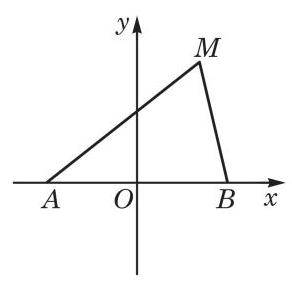
\includegraphics[max width=0.2\textwidth]{images/bo_d7fqvdc91nqc7381i9u0_81_1155_1191_292_283_0.jpg}
\end{center}
\hspace*{3em} 

图 2-5-1

设动点 \(M\) 的坐标是 \(\left( {x,y}\right)\) ,则 \(\overrightarrow{MA} = \left( {-2 - x, - y}\right) ,\overrightarrow{MB} = \; \left( {2 - x, - y}\right)\) . 因为 \(\overrightarrow{MA} \cdot  \overrightarrow{MB} = 5\) ,所以

\[
\left( {-2 - x}\right) \left( {2 - x}\right)  + \left( {-y}\right) \left( {-y}\right)  = 5,
\]

化简, 得

\[
{x}^{2} + {y}^{2} = 9
\]

这表明, 动点轨迹上任意点的坐标都满足这个方程.

反过来,设平面上一点 \(N\) 的坐标 \(\left( {{x}_{1},{y}_{1}}\right)\) 满足方程,即有 \({x}_{1}^{2} + {y}_{1}^{2} = 9\) ,则

\[
\overrightarrow{NA} \cdot  \overrightarrow{NB} = \left( {-2 - {x}_{1}}\right) \left( {2 - {x}_{1}}\right)  + \left( {0 - {y}_{1}}\right) \left( {0 - {y}_{1}}\right)
\]

\[
= {x}_{1}^{2} - 4 + {y}_{1}^{2} = 9 - 4 = 5\text{ . }
\]

从而,以方程 \({x}^{2} + {y}^{2} = 9\) 的解为坐标的点都在轨迹上.

综上所述,方程 \({x}^{2} + {y}^{2} = 9\) 就是所求的动点 \(M\) 的轨迹方程.

要证明一个给定的关于 \(x\text{ 、 }y\) 的方程是一条给定曲线的方程, 有时可以把条件 \circled{1} 和条件 \circled{2} 放在一起验证. 此时要验证的是如下的充要条件: 一点在给定曲线上当且仅当该点的坐标是给定方程的解.

例 3 求连接定点 \(A\left( {4,0}\right)\) 和曲线 \({x}^{2} + 2{y}^{2} = 1\) 上动点 \(B\) 的线段 \({AB}\) 的中点 \(P\) 的轨迹方程.

解 对平面上一点 \(B\left( {{x}_{B},{y}_{B}}\right)\) ,条件“ \(P\left( {{x}_{P},{y}_{P}}\right)\) 是线段 \({AB}\) 的中点”的坐标表示是 Q

\[
\left\{  {\begin{array}{l} {x}_{P} = \frac{4 + {x}_{B}}{2}, \\  {y}_{P} = \frac{0 + {y}_{B}}{2}, \end{array}\text{ 即 }\left\{  \begin{array}{l} {x}_{B} = 2{x}_{P} - 4, \\  {y}_{B} = 2{y}_{P}. \end{array}\right. }\right.
\]

\HRule

例 3 也可按步骤 2、3 证明，但不要忽略了步骤 3:假设点 \(P\) 的坐标是方程 \(4{\left( x - 2\right) }^{2} + 8{y}^{2} = 1\) 的解,要找到曲线 \({x}^{2} + \; 2{y}^{2} = 1\) 上的一点 \(B\) ,使 \(P\) 是线段 \({AB}\) 的中点.

\HRule

由所求轨迹的定义,点 \(P\left( {{x}_{P},{y}_{P}}\right)\) 在轨迹上当且仅当点 \(B\left( {{x}_{B},{y}_{B}}\right)\) 在曲线 \({x}^{2} + 2{y}^{2} = 1\) 上,即当且仅当 \({x}_{B}^{2} + 2{y}_{B}^{2} = 1\) . 把点 \(B\) 的坐标用点 \(P\) 的坐标替换并化简,得

\[
{x}_{B}^{2} + 2{y}_{B}^{2} = 1 \Leftrightarrow  4{\left( {x}_{P} - 2\right) }^{2} + 8{y}_{P}^{2} = 1,
\]

所以,点 \(P\) 在轨迹上当且仅当它的坐标是方程 \(4{\left( x - 2\right) }^{2} + 8{y}^{2} = 1\) 的解.

由此可见,所求的轨迹方程是 \(4{\left( x - 2\right) }^{2} + 8{y}^{2} = 1\) .

\section*{练习 2.5(1)}

1. 判断下列各组两个方程是否表示相同的曲线:

(1) \(y = x,\frac{y}{x} = 1\) ； (2) \(y = x,y = \sqrt{{x}^{2}}\) ； (3) \(\left| x\right|  = \left| y\right| ,{x}^{2} - {y}^{2} = 0\) .

2. 已知 \(\bigtriangleup  {ABC}\) 的周长为 18，且 \({BC} = 8\) . 建立适当的平面直角坐标系，求顶点 \(A\) 的轨迹方程.

3. 当点 \(A\) 在曲线 \(y = {x}^{2} + 3\) 上运动时,连接点 \(A\) 与定点 \(B\left( {6,0}\right)\) . 求 \({AB}\) 的中点 \(P\) 的轨迹方程.

\section*{2 简单的参数方程}

在求轨迹的方程时, 有时根据条件很难直接建立曲线上的动点坐标 \(\left( {x,y}\right)\) 所满足的方程,但如果引入合适的第三个变量,分别建立 \(x\text{ 、 }y\) 与第三个变量的联系,问题常常会比较容易得到解决.

我们先来看一个熟悉的问题: 假设空气阻力忽略不计，求炮弹被击发后的运动轨迹的方程.

即使建立平面直角坐标系, 炮弹的运动规律也难以直接用炮弹位置的坐标 \(x\) 与 \(y\) 的方程表示出来. 在物理学中，我们知道，当发射角 \(\alpha\) 、发射时的初速度 \({v}_{0}\) 确定后,炮弹位置只与运行时间 \(t\) 有关, 所以可以考虑引入时间 \(t\) 作为第三个变量来求运动轨迹的方程.

以炮口所在位置 \(O\) 为坐标原点,水平方向为 \(x\) 轴,铅垂方向为 \(y\) 轴,建立平面直角坐标系,如图 2-5-2 所示. 设炮弹发射 \(t\) s后的位置在点 \(P\left( {x,y}\right)\) 处. 炮弹的初速度 \({v}_{0}\) 可分解为水平方向和铅垂方向的两个速度,其中在水平方向上的初速度为 \({v}_{0}\cos \alpha\) , 在铅垂方向上的初速度为 \({v}_{0}\sin \alpha\) . 由于忽略了空气阻力,炮弹在运动过程中只在铅垂方向受到重力作用. 容易求得，炮弹的位置坐标 \(\left( {x,y}\right)\) 与时间 \(t\) 之间的关系:

\[
\left\{  {\begin{array}{l} x = {v}_{0}t\cos \alpha , \\  y = {v}_{0}t\sin \alpha  - \frac{1}{2}g{t}^{2} \end{array}\left( {0 \leq  t \leq  {t}_{1}}\right) ,}\right.
\]

\begin{center}
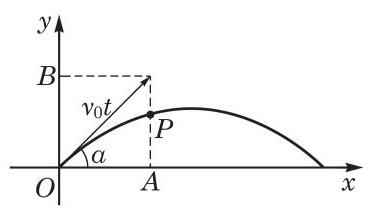
\includegraphics[max width=0.3\textwidth]{images/bo_d7fqvdc91nqc7381i9u0_83_1116_400_368_213_0.jpg}
\end{center}
\hspace*{3em} 

图 2-5-2

其中 \(g\) 是重力加速度的值, \({t}_{1}\) 是炮弹击中目标的时刻.

我们把上述方程组中的变量 \(t\) 消去后,观察它表示的是什么曲线. 由第一个方程得 \(t = \frac{x}{{v}_{0}\cos \alpha }\) ,代入第二个方程,消去参数 \(t\) ,得到炮弹运动的轨迹方程为

\[
y =  - \frac{g}{2{v}_{0}^{2}{\cos }^{2}\alpha }{x}^{2} + \frac{\sin \alpha }{\cos \alpha }x.
\]

由于 \({v}_{0}\text{ 、 }\alpha \text{ 、 }g\) 都是定值,因此炮弹运动的轨迹是一条抛物线.

在这个实际问题中, 炮弹运动的轨迹不可能是整条抛物线. 首先,因为炮弹被击发前是静止的,必须 \(x \geq  0\) . 又因为炮弹击中目标后也不再按原有轨迹运动，所以我们所讨论的炮弹运动轨迹只是 \(x \geq  0\) 与炮弹击中目标前的一段抛物线. 例如，设目标点与发射点在同一水平线上,则恒有 \(y \geq  0\) ,从而由 \(- \frac{g}{2{v}_{0}^{2}{\cos }^{2}\alpha }{x}^{2} + \; \frac{\sin \alpha }{\cos \alpha }x \geq  0\) 求得 \(x \leq  \frac{{v}_{0}^{2}\sin {2\alpha }}{g}\) . 因此,炮弹运动轨迹是上述抛物线在 \(0 \leq  x \leq  \frac{{v}_{0}^{2}\sin {2\alpha }}{g}\) 之间的部分.

由上述讨论可以看到, 在求曲线方程时, 我们可以先分别求出 \(x\text{ 、 }y\) 与某个随动点变化的变量 \(t\) 所满足的方程 \(x = f\left( t\right)\) , \(y = g\left( t\right)\) ,得到方程组:

\[
\left\{  \begin{array}{l} x = f\left( t\right) , \\  y = g\left( t\right) , \end{array}\right.
\]

其中 \(t\) 在某个范围内变动.

如果对于 \(t\) 的每一个允许值,由上述方程组所确定的点 \(P\left( {x,y}\right)\) 都在曲线 \(C\) 上; 反之,对于曲线 \(C\) 上任意一点的坐标, 都存在 \(t\) 的某个允许值使得上述方程组成立,那么上述方程组就叫做曲线 \(C\) 的参数方程 (parametric equation),变量 \(t\) 叫做参变量或参数 (parameter).

相对于参数方程而言,直接给出曲线上点的坐标 \(x\text{ 、 }y\) 之间关系的方程 \(F\left( {x,y}\right)  = 0\) 叫做曲线的普通方程. 如果像上例那样可以消去参数方程中的参数 \(t\) ,就可以将参数方程化为普通方程.

但在不少情况下，由曲线的参数方程并不一定能够化为曲线的普通方程. 举一个通俗的例子. 假设有一只小虫在平面直角坐标系中爬行,小虫的位置坐标 \(\left( {x,y}\right)\) 是时间 \(t\) 的函数:

\[
\left\{  \begin{array}{l} x = f\left( t\right) , \\  y = g\left( t\right) . \end{array}\right.
\]

这揭示了小虫随时间 \(t\) 变化的运动规律,就是小虫运动轨迹的一个参数方程. 由于小虫爬行的轨迹不似炮弹那样一直向前, 而是可以倒退及与自身相交, 不可能化为普通方程, 这时, 用参数方程来表示这一复杂的运动轨迹就成了唯一合理的选择了.

由此可见, 用参数方程表示一个曲线, 不仅可能有具体的物理或几何意义, 也更具有一般性, 应用起来有时也更为简便.

\begin{center}
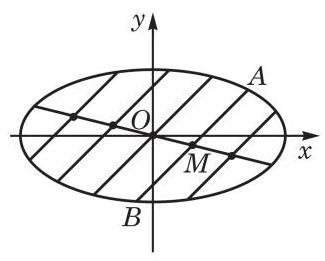
\includegraphics[max width=0.2\textwidth]{images/bo_d7fqvdc91nqc7381i9u0_84_186_1366_325_261_0.jpg}
\end{center}
\hspace*{3em} 

图 2-5-3

例 4 求所有斜率为 1 的直线被椭圆 \(\frac{{x}^{2}}{4} + {y}^{2} = 1\) 所截得的线段的中点的轨迹.

解 如图 2-5-3,设直线 \(y = x + b\) 被椭圆所截得的线段的两个端点 \(A\text{ 、 }B\) 的坐标 \(\left( {{x}_{1},{y}_{1}}\right) \text{ 、 }\left( {{x}_{2},{y}_{2}}\right)\) 是如下方程组的解:

\[
\left\{  \begin{array}{l} \frac{{x}^{2}}{4} + {y}^{2} = 1, \\  y = x + b. \end{array}\right.
\]

消去 \(y\) ,并整理得

\[
5{x}^{2} + {8bx} + 4\left( {{b}^{2} - 1}\right)  = 0.
\]

当判别式 \(\Delta  = {\left( 8b\right) }^{2} - 4 \times  5 \times  4\left( {{b}^{2} - 1}\right)  =  - {16}\left( {{b}^{2} - 5}\right)  > 0\) ,即 \(- \sqrt{5} < b < \sqrt{5}\) 时,上述方程有两个不同的实数解,即直线被椭圆所截的线段存在并且线段两个端点横坐标之和为 \({x}_{1} + {x}_{2} =  - \frac{8}{5}b\) .

设 \({AB}\) 的中点为 \(M\left( {{x}_{M},{y}_{M}}\right)\) ,则

\[
{x}_{M} = \frac{{x}_{1} + {x}_{2}}{2} =  - \frac{4}{5}b,{y}_{M} = {x}_{M} + b = \frac{b}{5}.
\]

所以,

\[
\left\{  \begin{array}{l} {x}_{M} =  - \frac{4}{5}b, \\  {y}_{M} = \frac{b}{5}\;\left( {-\sqrt{5} < b < \sqrt{5}}\right)  \end{array}\right.
\]

就是线段 \({AB}\) 的中点 \(M\) 的轨迹的参数方程.

消去 \(b\) ,得 \({x}_{M} + 4{y}_{M} = 0\) . 由 \(- \sqrt{5} < b < \sqrt{5}\) 及 \({x}_{M} =  - \frac{4b}{5}\) ,可得 \({x}_{M} \in  \left( {-\frac{4\sqrt{5}}{5},\frac{4\sqrt{5}}{5}}\right)\) . 所以点 \(M\) 的轨迹方程为 \(x + {4y} = 0\) , \(x \in  \left( {-\frac{4\sqrt{5}}{5},\frac{4\sqrt{5}}{5}}\right)\) ,即点 \(M\) 的轨迹是直线 \(x + {4y} = 0\) 在椭圆内的部分.

例 5 已知点 \(M\left( {x,y}\right)\) 在椭圆 \(C : \frac{{x}^{2}}{16} + \frac{{y}^{2}}{9} = 1\) 上，求 \(x + y\) 的最大值,并求 \(x + y\) 取得最大值时点 \(M\) 的坐标.

解 利用三角恒等式 \({\cos }^{2}\theta  + {\sin }^{2}\theta  = 1\) ,可以验证

\[
\left\{  {\begin{array}{l} x = 4\cos \theta , \\  y = 3\sin \theta , \end{array}\;\theta  \in  \mathbf{R}}\right.
\]

是椭圆 \(C\) 的一个参数方程,所以点 \(M\) 的坐标满足

\[
x + y = 4\cos \theta  + 3\sin \theta  = 5\left( {\frac{4}{5}\cos \theta  + \frac{3}{5}\sin \theta }\right) .
\]

因为 \({\left( \frac{4}{5}\right) }^{2} + {\left( \frac{3}{5}\right) }^{2} = 1\) ,所以可以找到锐角 \(\varphi\) ,使得 \(\sin \varphi  = \frac{4}{5}\) , \(\cos \varphi  = \frac{3}{5}\) ,从而

\[
x + y = 5\left( {\sin \varphi \cos \theta  + \cos \varphi \sin \theta }\right)  = 5\sin \left( {\theta  + \varphi }\right) .
\]

当 \(\sin \left( {\theta  + \varphi }\right)  = 1\) 时, \(x + y = 5\) 最大. 要取得最大值, \(\theta  + \varphi  = \; \frac{\pi }{2} + {2k\pi }\) ,即 \(\theta  = \frac{\pi }{2} + {2k\pi } - \varphi\) ,这里 \(k \in  \mathbf{Z}\) . 此时对应的点 \(M\) 的坐标为 \(x = 4\cos \theta  = 4\sin \varphi  = \frac{16}{5},y = 3\sin \theta  = 3\cos \varphi  = \frac{9}{5}\) ,即点 \(M\) 的坐标为 \(\left( {\frac{16}{5},\frac{9}{5}}\right)\) .

\HRule

还可用什么方法求解例 4 ?

\HRule

\section*{练习 2.5(2)}

1. 设 \(a\text{ 、 }b\) 是非零常数,参数方程 \(\left\{  {\begin{array}{l} x = \frac{a}{\cos \alpha }, \\  y = b\tan \alpha  \end{array}\left( {\alpha  \neq  {k\pi } + \frac{\pi }{2},k \in  \mathbf{Z}}\right) }\right.\) 表示的是什么曲线?

2. 以原点为圆心、1 为半径作一个圆. 设定点 \(A\) 的坐标为 \(\left( {2,0}\right) ,B\) 为圆上任意一点, \(M\) 为线段 \({AB}\) 的中点. 求点 \(M\) 轨迹的参数方程.

3. 动点 \(M\) 作匀速直线运动,它在 \(x\) 轴和 \(y\) 轴方向的分速度分别为 9 和 12,运动开始时,点 \(M\) 位于 \(A\left( {1,1}\right)\) . 求点 \(M\) 的轨迹的参数方程.

\section*{3 极坐标系与极坐标方程}

通过前面的学习，我们知道，在平面直角坐标系下，可以用一对有序实数表示平面上点的位置，进而建立曲线的直角坐标方程, 从而用代数方法研究这些曲线的性质. 但是, 有些简单的曲线, 在用上述方法求它的方程时, 却会遇到比较大的困难. 例如,设想平面上有一个动点 \(M\) 在一条从点 \(O\) 出发的射线 \({OA}\) 上做匀速运动逐渐远离点 \(O\) ，而射线 \({OA}\) 本身又绕点 \(O\) 以固定的角速度旋转. 此时，动点 \(M\) 在平面上的运动轨迹称为等速螺线 (图 2-5-4)，它在数学内部以及机械、工程等领域有广泛的应用. 如图 2-5-5 所示的由两条对称的等速螺线拼成的心形转轮 (红线所示)就会把转轮的旋转运动转化为横杆(蓝线所示)的往复水平运动.

\begin{center}
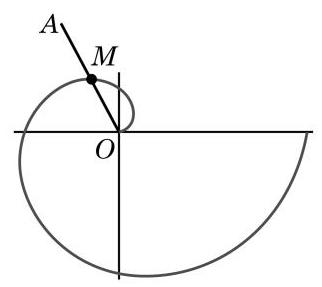
\includegraphics[max width=0.2\textwidth]{images/bo_d7fqvdc91nqc7381i9u0_86_186_1052_322_287_0.jpg}
\end{center}
\hspace*{3em} 

图 2-5-4

\begin{center}
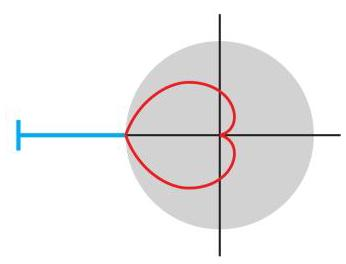
\includegraphics[max width=0.2\textwidth]{images/bo_d7fqvdc91nqc7381i9u0_86_171_1414_346_264_0.jpg}
\end{center}
\hspace*{3em} 

图 2-5-5

事实上, 确定平面上点的位置, 采用平面直角坐标系并不是唯一的方法. 现实生活中, 人们也常用方向 (实际上是角) 和距离来确定平面上点的位置. 例如, 图 2-5-6 所示的是雷达上发现北

\begin{center}
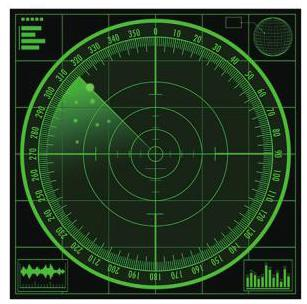
\includegraphics[max width=0.2\textwidth]{images/bo_d7fqvdc91nqc7381i9u0_86_194_1789_307_304_0.jpg}
\end{center}
\hspace*{3em} 

图 2-5-6

但是, 在平面直角坐标下要建立等速螺线的方程是一件比较复杂的事:把两点的距离用点的坐标写出, 需要用到二次根式; 而把旋转角用坐标表示出来, 更要借助于反三角函数. 因此, 研究等速螺线及其他类似曲线, 需要另辟蹊径. 偏西 \({45}^{ \circ  }\) 方向 \({20}\mathrm{\;{km}}\) 处有不明飞行物体. 这样表示平面上点的位置就是我们将要研究的另外一种坐标系——极坐标系的基本思想.

如图 2-5-7,在平面上取一定点 \(O\) ,以 \(O\) 为端点引射线 \({Ox}\) , 再选定一个单位长度和旋转角的正方向 (一般规定逆时针方向为正方向). 这时对于平面上异于点 \(O\) 的任意一点 \(M\) ,设 \(\rho  = \; \left| {OM}\right| ,\theta\) 表示以射线 \({Ox}\) 为始边、射线 \({OM}\) 为终边的角,则点 \(M\) 的位置可以用有序数对 \(\left( {\rho ,\theta }\right)\) 表示. 我们把这样的坐标系叫做极坐标系(polar coordinate system).

\begin{center}
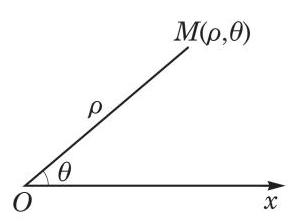
\includegraphics[max width=0.2\textwidth]{images/bo_d7fqvdc91nqc7381i9u0_87_1159_421_290_221_0.jpg}
\end{center}
\hspace*{3em} 

图 2-5-7

在极坐标系中,定点 \(O\) 叫做极点 (pole),射线 \({Ox}\) 叫做极轴 (polar axis), \(\left( {\rho ,\theta }\right)\) 就叫做点 \(M\) 的极坐标 (polar coordinate),其中 \(\rho\) 叫做点 \(M\) 的极径 (polar radius), \(\theta\) 叫做点 \(M\) 的极角 (polar angle).

与平面直角坐标系不一样的是, 在极坐标系中, 点的极坐标不唯一,如果 \(\left( {\rho ,\theta }\right)\) 是一点的极坐标,那么 \(\left( {\rho ,\theta  + {2n\pi }}\right) \left( {n \in  \mathbf{Z}}\right)\) 都可以作为它的极坐标. 我们还允许 \(\rho\) 取负值,当 \(\rho  < 0\) 时,规定 \(\left( {\rho ,\theta }\right)\) 对应的点为 \(\left( {-\rho ,\theta  + \pi }\right)\) . 此外,规定极点的坐标为 \(\left( {0,\theta }\right)\) , 其中 \(\theta\) 可以是任意角.

不难发现,在极坐标系中,点 \(\left( {\rho ,\theta }\right)\) 与 \(\left( {-\rho ,\theta }\right)\) 关于极点对称,点 \(\left( {\rho ,\theta }\right)\) 与 \(\left( {\rho , - \theta }\right)\) 关于极轴对称.

尽管在极坐标系中点的坐标不唯一, 但是在极坐标系中, 除了极点外，平面上的所有点所成的集合和实数对集合 \(\{ \left( {\rho ,\theta }\right)  \mid  \rho  > 0,0 \leq  \theta  < {2\pi }\}\) 是一一对应的. 也就是说,如果规定极径 \(\rho\) 取正值,极角 \(\theta\) 取小于 \({2\pi }\) 的非负值,那么极点以外的任何点的极坐标也就唯一确定了.

\begin{center}
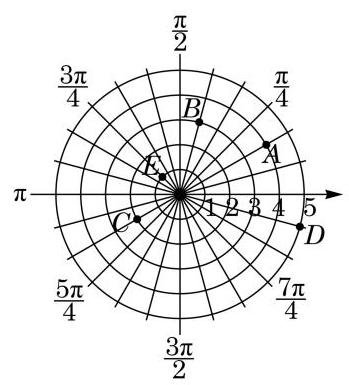
\includegraphics[max width=0.2\textwidth]{images/bo_d7fqvdc91nqc7381i9u0_87_1131_1582_349_385_0.jpg}
\end{center}
\hspace*{3em} 

图 2-5-8

例 6 如图 2-5-8,在极坐标系中,写出 \(A\text{ 、 }B\text{ 、 }C\text{ 、 }D\) 、 \(E\) 各点的一个极坐标.

解 \(A\text{ 、 }B\text{ 、 }C\text{ 、 }D\text{ 、 }E\) 各点的一个极坐标可分别取为 \(\left( {4,\frac{\pi }{6}}\right)\) 、 \(\left( {3,\frac{5\pi }{12}}\right) \text{ 、 }\left( {2,\frac{7\pi }{6}}\right) \text{ 、 }\left( {5,\frac{23\pi }{12}}\right) \text{ 、 }\left( {1,\frac{3\pi }{4}}\right) .\)

\section*{练习 2.5(3)}

\begin{center}
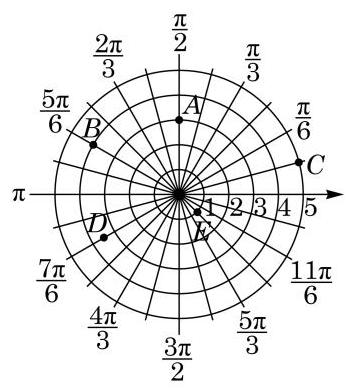
\includegraphics[max width=0.2\textwidth]{images/bo_d7fqvdc91nqc7381i9u0_88_1151_309_346_388_0.jpg}
\end{center}
\hspace*{3em} 

(第 1 题)

1.(1)若约定 \(\rho  > 0,0 \leq  \theta  < {2\pi }\) ，试写出图中 \(A\) 、 \(B\) 、 \(C\) 、 \(D\text{ 、 }E\) 各点的极坐标 \(\left( {\rho ,\theta }\right)\) ;

(2)若约定 \(\rho  < 0,0 \leq  \theta  < {2\pi }\) ，试写出图中 \(A\) 、 \(B\) 、 \(C\) 、 \(D\) 、 \(E\) 各点的极坐标 \(\left( {\rho ,\theta }\right)\) .

2. 在极坐标系中,画出点 \(A\left( {3,\frac{\pi }{4}}\right) \text{ 、 }B\left( {3, - \frac{\pi }{4}}\right) \text{ 、 }C\left( {3,\frac{5\pi }{4}}\right)\) , 并说明 \(A\) 和 \(B\text{ 、 }C\) 有怎样的位置关系.

和平面直角坐标系的情形类似, 在极坐标系中, 平面上的一条曲线可以用含 \(\rho \text{ 、 }\theta\) 这两个变量的方程 \(F\left( {\rho ,\theta }\right)  = 0\) 来表示,方程 \(F\left( {\rho ,\theta }\right)  = 0\) 叫做这条曲线的极坐标方程. 此时,曲线和方程有如下的关系:

?

(1)以方程 \(F\left( {\rho ,\theta }\right)  = 0\) 的解为极坐标的点都在曲线上;

\HRule

在(2)中，为什么不说曲线上每一点的所有极坐标都适合方程?

\HRule

(2)曲线上每一点的所有极坐标中，至少有一个极坐标 \(\left( {\rho ,\theta }\right)\) 是方程 \(F\left( {\rho ,\theta }\right)  = 0\) 的解.

求曲线的极坐标方程, 其实就是找到曲线上所有点的极径和极角应满足的关系式.

例 7 求圆心是 \(C\left( {a,0}\right)\) 、半径是 \(a\) 的圆的极坐标方程.

\begin{center}
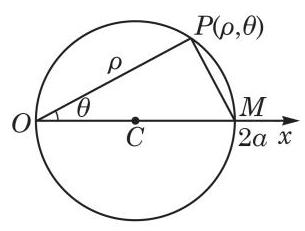
\includegraphics[max width=0.2\textwidth]{images/bo_d7fqvdc91nqc7381i9u0_88_196_1565_305_231_0.jpg}
\end{center}
\hspace*{3em} 

图 2-5-9

解 如图 2-5-9,由题意知圆 \(C\) 经过极点 \(O\) . 设圆和极轴的另一个交点是 \(M\) ,则 \(\left| {OM}\right|  = {2a}\) . 设 \(P\left( {\rho ,\theta }\right) \left( {-\frac{\pi }{2} < \theta  \leq  \frac{\pi }{2}}\right)\) 是圆 \(C\) 上的任意一点.

若点 \(P\) 不在直线 \({OM}\) 上,因为 \({OM}\) 是圆的直径,所以 \(\angle {OPM}\) 为直角. 在直角三角形 \({OPM}\) 中, \(\left| {OP}\right|  = \left| {OM}\right| \cos \theta\) ,即

\[
\rho  = {2a}\cos \theta \text{ ,这里 } - \frac{\pi }{2} < \theta  < \frac{\pi }{2},\theta  \neq  0\text{ . }
\]

当 \(\theta  = 0\) 与 \(\theta  = \frac{\pi }{2}\) 时,方程 \(\rho  = {2a}\cos \theta\) 分别给出了点 \(M\) 与点 \(O\) .

因此,圆 \(C\) 的极坐标方程是

\[
\rho  = {2a}\cos \theta \left( {-\frac{\pi }{2} < \theta  \leq  \frac{\pi }{2}}\right) .
\]

\begin{center}
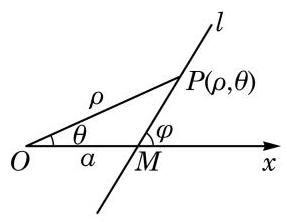
\includegraphics[max width=0.2\textwidth]{images/bo_d7fqvdc91nqc7381i9u0_89_1158_277_287_222_0.jpg}
\end{center}
\hspace*{3em} 

图 2-5-10

例 8 如图 2-5-10,求经过点 \(M\left( {a,0}\right) \left( {a > 0}\right)\) ,且与极轴夹角为 \(\varphi\) 的直线 \(l\) 的极坐标方程.

解 设 \(P\left( {\rho ,\theta }\right)\) 是直线 \(l\) 上位于点 \(M\) 上方的任意一点,则

\[
\left| {OP}\right|  = \rho ,\angle {POx} = \theta \left( {0 < \theta  < \varphi }\right) ,\angle {OPM} = \varphi  - \theta .
\]

在 \(\bigtriangleup {POM}\) 中,由正弦定理,得

即

\[
\frac{\rho }{\sin \left( {\pi  - \varphi }\right) } = \frac{a}{\sin \left( {\varphi  - \theta }\right) },
\]

\[
\rho \sin \left( {\varphi  - \theta }\right)  = a\sin \varphi
\]
  \circled{1} 

?

\HRule

若 \(\varphi  = \frac{\pi }{2}\) ,直线 \(l\) 的方程变成怎样?

\HRule

当点 \(P\) 位于点 \(M\) 下方或与点 \(M\) 重合时,同样可推得 \circled{1} .

因此,方程 \circled{1} 就是所求直线 \(l\) 的极坐标方程.

我们不仅可以建立圆、直线的极坐标方程, 也可以建立圆锥曲线的极坐标方程(见课后阅读). 下面，我们尝试建立上一小节开头时给出的等速螺线的极坐标方程.

\begin{center}
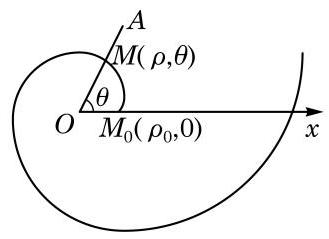
\includegraphics[max width=0.2\textwidth]{images/bo_d7fqvdc91nqc7381i9u0_89_1137_1056_329_239_0.jpg}
\end{center}
\hspace*{3em} 

图 2-5-11

例 9 设质点 \(M\) 为射线 \({OA}\) 上的动点,沿着 \(\overrightarrow{OA}\) 方向做匀速运动，同时射线 \({OA}\) 又绕着它的端点 \(O\) 作等角速度旋转. 求质点 \(M\) 运动的轨迹方程.

解 如图 2-5-11,以射线 \({OA}\) 的端点 \(O\) 为极点,以射线 \({OA}\) 的初始位置为极轴,建立极坐标系. 设动点的初始位置是 \({M}_{0}\left( {{\rho }_{0},0}\right)\) , 点 \(M\) 在 \({OA}\) 上运动的速度为 \(v,{OA}\) 绕点 \(O\) 转动的角速度为 \(\omega\) , 经过时间 \(t\) 后,动点到达的位置为 \(M\left( {\rho ,\theta }\right)\) .

因为点 \(M\) 沿 \({OA}\) 做匀速运动,所以

Q

\[
\rho  = {\rho }_{0} + {vt};
\]
  \circled{1} 

\HRule

 \circled{1} 和 \circled{2} 联立实际上就是此运动轨迹的参数方程.

\HRule

由射线 \({OA}\) 绕点 \(O\) 作等角速度旋转,得

\[
\theta  = {\omega t}.
\]
  \circled{2} 

由于从点 \({M}_{0}\) 到点 \(M\) 是直线运动与旋转运动的合成,因此将从 \circled{2} 式得到的 \(t = \frac{\theta }{\omega }\) 代入 \circled{1} 式，得

\[
\rho  = {\rho }_{0} + \frac{v}{\omega } \cdot  \theta ,
\]

其中 \({\rho }_{0}\text{ 、 }v\text{ 、 }\omega\) 为常数. 设 \(\frac{v}{\omega } = a\) ,则方程可写成

\[
\rho  = {\rho }_{0} + {a\theta }\left( {\theta  \geq  0}\right) .
\]

这就是所求轨迹的极坐标方程.

这个方程所对应的曲线 (图 2-5-11) 叫做等速螺线或者叫做

阿基米德螺线 (Archimedean spiral). 当 \({\rho }_{0} = 0\) 时,就得到特殊的等速螺线的方程 \(\rho  = {a\theta }\) ,此时极径与极角成正比.

\section*{练习 2.5(4)}

1. 求经过点 \(A\left( {a,0}\right)\) 且和极轴垂直的直线 \(l\) 的极坐标方程.

2.(1)求圆心在极点 \(O\) 、半径为 \(a\) 的圆的极坐标方程；

(2)求圆心在 \(\left( {a,\frac{\pi }{2}}\right)\) 、半径为 \(a\) 的圆的极坐标方程.

3. 分别画出下列极坐标方程和直角坐标方程的曲线:

(1)极坐标方程 \(\rho  = 2\) ，直角坐标方程 \(x = 2\) ；

(2)极坐标方程 \(\theta  = \frac{\pi }{4}\) ，直角坐标方程 \(x = \frac{\pi }{4}\) .

\section*{4 极坐标与直角坐标的互化}

\begin{center}
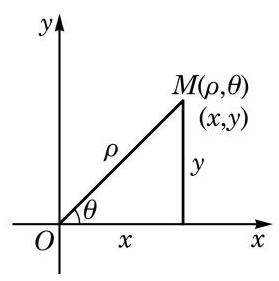
\includegraphics[max width=0.2\textwidth]{images/bo_d7fqvdc91nqc7381i9u0_90_218_1166_279_281_0.jpg}
\end{center}
\hspace*{3em} 

图 2-5-12

极坐标系和直角坐标系是两种不同的坐标系, 有时需要在它们之间进行互相转化.

如图 2-5-12,把直角坐标系的原点作为极点, \(x\) 轴的正半轴作为极轴,并且取相同的单位长度. 设平面上任意一点 \(M\) 的直角坐标为 \(\left( {x,y}\right)\) ,极坐标为 \(\left( {\rho ,\theta }\right)\) .

当 \(\rho  > 0\) 时,由三角函数的定义,可以得到如下的关系式:

\[
x = \rho \cos \theta ,y = \rho \sin \theta .
\]
  \circled{1} 

当 \(\rho  = 0\) 时, \circled{1} 式仍然成立.

\begin{center}
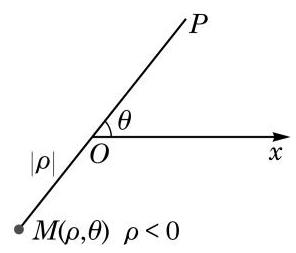
\includegraphics[max width=0.2\textwidth]{images/bo_d7fqvdc91nqc7381i9u0_90_197_1619_296_253_0.jpg}
\end{center}
\hspace*{3em} 

图 2-5-13

当 \(\rho  < 0\) 时,如图 2-5-13,点 \(M\) 的极坐标也可用 \(\left( {-\rho ,\pi  + \theta }\right)\) 表示,这时由于 \(- \rho  > 0\) ,因此由三角函数的定义,可得

\[
x =  - \rho \cos \left( {\pi  + \theta }\right)  = \rho \cos \theta ,
\]

\[
y =  - \rho \sin \left( {\pi  + \theta }\right)  = \rho \sin \theta .
\]

这说明 \(\rho  < 0\) 时, \circled{1} 式也成立.

综上所述,关系式 \circled{1} 对于点 \(M\) 的任一种表示法表示的极坐标都成立.

关系式 \circled{1} 可以作为已知点的极坐标求该点的直角坐标的公式.

从关系式 \circled{1} 中解出 \(\rho\) 、 \(\theta\) ,则有

\[
{\rho }^{2} = {x}^{2} + {y}^{2},\tan \theta  = \frac{y}{x}\left( {x \neq  0}\right) .
\]
  \circled{2} 

关系式 \circled{2} 可以作为已知点的直角坐标求该点的极坐标的公式.

通常取 \(\rho\) 为正数,即 \(\rho  = \sqrt{{x}^{2} + {y}^{2}}\) ; 由 \(\tan \theta  = \frac{y}{x}\) 确定角度 \(\theta\) 时,一般根据此点所在的象限取最小正角,满足 \(0 \leq  \theta  < {2\pi }\) .

例 10 化直角坐标方程 \(x - y = 0\) 为极坐标方程.

解 将 \(x = \rho \cos \theta ,y = \rho \sin \theta\) 代入 \(x - y = 0\) ,得

\[
\rho \cos \theta  - \rho \sin \theta  = 0,
\]

即

\[
\rho \left( {\cos \theta  - \sin \theta }\right)  = 0.
\]

解得

\[
\rho  = 0\text{ 或 }\cos \theta  - \sin \theta  = 0.
\]

由 \(\cos \theta  - \sin \theta  = 0\) ,得 \(\tan \theta  = 1\) .

解得

\[
\theta  = \frac{\pi }{4}\text{ 或 }\theta  = \frac{5\pi }{4}.
\]

因为 \(\rho  = 0\) 表示极点,而 \(\theta  = \frac{\pi }{4}\) 及 \(\theta  = \frac{5\pi }{4}\) 均表示过极点的射线,所以 \(\rho  = 0\) 已包含在 \(\theta  = \frac{\pi }{4}\) 或 \(\theta  = \frac{5\pi }{4}\) 中.

因此,所化的极坐标方程为 \(\theta  = \frac{\pi }{4}\) 或 \(\theta  = \frac{5\pi }{4}\) .

例 11 化极坐标方程 \(\rho  = 4\cos \theta\) 为直角坐标方程,并指出它是什么曲线.

解 当 \(\rho  \neq  0\) 时,由 \(\rho  = 4\cos \theta\) ,得

\[
{\rho }^{2} = {4\rho }\cos \theta .
\]

由此得 \({x}^{2} + {y}^{2} = {4x}\) ,即

\[
{\left( x - 2\right) }^{2} + {y}^{2} = 4\text{ . }
\]
  \circled{1} 

当 \(\rho  = 0\) 时,满足 \(\rho  = 4\cos \theta\) 的点为极点,即直角坐标系的原点 \(\left( {0,0}\right)\) ,它也满足方程 \circled{1} .

所以, \(\rho  = 4\cos \theta\) 是以 \(\left( {2,0}\right)\) 为圆心、以 2 为半径的圆.

\section*{练习 2.5(5)}

1. ( 1 )把点 \(M\) 的极坐标 \(\left( {2,\frac{\pi }{6}}\right)\) 化成直角坐标；

(2)把点 \(P\) 的直角坐标 \(\left( {-1,\sqrt{3}}\right)\) 化成极坐标.

\HRule

如果允许 \(\rho\) 取任意实数,那么极坐标方程 \(\theta  = \frac{\pi }{4}\) 及 \(\theta  = \frac{5\pi }{4}\) 均表示过极点的直线.

\HRule

2. 化直角坐标方程 \({x}^{2} + {y}^{2} - {2ay} = 0\) 为极坐标方程.

3. 化极坐标方程 \(\rho  = \sin \theta  + \cos \theta\) 为直角坐标方程.

\section*{课后阅读}

\section*{圆锥曲线的统一定义及其极坐标方程}

在极坐标系中可以给出圆锥曲线的一个简洁的统一方程. 不过, 圆不能被这个统一方程包括, 所以本阅读材料中的圆锥曲线不包括圆.

先讨论一下圆锥曲线的统一定义.

回忆一下抛物线的定义: 给定平面上的一个定点和一条定直线, 抛物线是该平面上到此定点和到此定直线距离相等的点的轨迹, 也就是说, 抛物线是该平面上到此定点和到此定直线距离之比等于 1 的点的轨迹. 我们知道, 给定的定点是抛物线的焦点, 给定的定直线是抛物线的准线.

我们希望模仿抛物线的这一定义给出椭圆的定义. 暂时在直角坐标系中讨论. 设椭圆的一个焦点为 \(F\left( {c,0}\right)\) ,长半轴长为 \(a\) ,则一点 \(M\left( {x,y}\right)\) 在椭圆上当且仅当

\[
\sqrt{{\left( x + c\right) }^{2} + {y}^{2}} + \sqrt{{\left( x - c\right) }^{2} + {y}^{2}} = {2a}.
\]

由于圆不在考虑范围内, \(c \neq  0\) ,上式经变形化为等价条件

\[
\frac{\sqrt{{\left( x - c\right) }^{2} + {y}^{2}}}{\left| x - \frac{{a}^{2}}{c}\right| } = e,
\]

其中 \(e = \frac{c}{a}\) 是椭圆的离心率,我们还把直线 \(l : x = \frac{{a}^{2}}{c}\) 称为椭圆的准线. 这样,上式用文字叙述就是: 椭圆是到焦点 \(F\left( {c,0}\right)\) 与到准线 \(l : x = \frac{{a}^{2}}{c}\) 的距离之比等于离心率 \(e\) 的点的轨迹,其中离心率满足 \(0 < e < 1\) .

由类似的推导过程可知,双曲线是到焦点 \(F\left( {c,0}\right)\) 与到准线 \(l : x = \frac{{a}^{2}}{c}\) 的距离之比等于离心率 \(e\) 的点的轨迹,此时离心率 \(e > 1\) .

由此,可以得到圆锥曲线的一个统一定义: 圆锥曲线是到一个定点 \(F\) 和到一条定直线 \(l\left( {F \notin  l}\right)\) 距离之比为定值 \(e\) 的点的轨迹. 其中,当 \(0 < e < 1\) 时,轨迹为椭圆; 当 \(e = 1\) 时,轨迹为抛物线; 当 \(e > 1\) 时,轨迹为双曲线.

据此定义可以建立圆锥曲线的统一极坐标方程.

设定点 \(F\) 到定直线 \(l\) 的距离为 \(p\left( {p > 0}\right)\) ,过定点 \(F\) 作定直线 \(l\) 的垂线,垂足为 \(K\) . 如图 2-5-14,以定点 \(F\) 为极点 \(O\) ,以 \({FK}\) 的反向延长线 \({Fx}\) 为极轴, 建立极坐标系.

\begin{center}
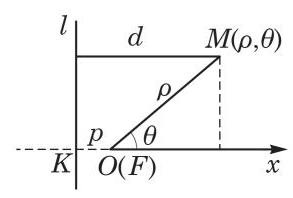
\includegraphics[max width=0.2\textwidth]{images/bo_d7fqvdc91nqc7381i9u0_93_1173_232_293_198_0.jpg}
\end{center}
\hspace*{3em} 

图 2-5-14

设动点 \(M\) 的极坐标为 \(\left( {\rho ,\theta }\right)\) ,则点 \(M\) 到定直线 \(l\) 的距离为

\[
d = p + \rho \cos \theta ,
\]

而 \(\left| {MF}\right|  = \rho\) ,由圆锥曲线的统一定义,有 \(\frac{\left| MF\right| }{d} = e\) ,可得 \(\rho  = {ed} = \; e\left( {p + \rho \cos \theta }\right)\) ,整理可得

\[
\rho  = \frac{ep}{1 - e\cos \theta }.
\]

这就是圆锥曲线的统一极坐标方程. 如图 2-5-15,当 \(0 < e < 1\) 时, 方程表示左焦点在极点的椭圆; 当 \(e = 1\) 时,方程表示焦点在极点,开口向右的抛物线; 当 \(e > 1\) 时,方程表示右焦点在极点的双曲线的右支.

\begin{center}
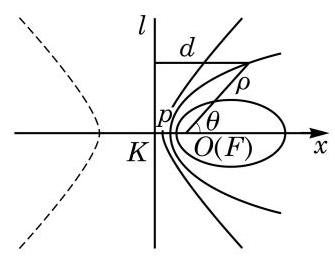
\includegraphics[max width=0.2\textwidth]{images/bo_d7fqvdc91nqc7381i9u0_93_1135_729_335_257_0.jpg}
\end{center}
\hspace*{3em} 

图 2-5-15

\section*{习题 2.5}

\section*{A 组}

1. 写出椭圆方程推导过程中的“反过来推演”，即验证:若点 \(M\) 以方程 \(\frac{{x}^{2}}{{a}^{2}} + \frac{{y}^{2}}{{b}^{2}} = 1 \; \left( {a > b > 0}\right)\) 的解 \(\left( {x,y}\right)\) 为坐标,则点 \(M\) 一定在以 \({F}_{1}\left( {-c,0}\right)\) 与 \({F}_{2}\left( {c,0}\right)\) 为焦点的椭圆上, 这里 \(c = \sqrt{{a}^{2} - {b}^{2}}\) .

2. 给定 \(A\left( {-3,2}\right) \text{ 、 }B\left( {3, - 2}\right)\) 两点,求证: 与这两点距离相等的点 \(P\) 的轨迹方程是 \({3x} - {2y} = 0.\)

3. 已知点 \(P\left( {2,1}\right)\) 在方程 \({x}^{2} + {k}^{2}{y}^{2} - {3x} - {ky} - 4 = 0\) 所表示的曲线上,求实数 \(k\) 的值.

4. 定长为 4 的线段 \({AB}\) 的两端点分别在 \(x\) 轴、 \(y\) 轴上滑动,求 \({AB}\) 中点的轨迹方程.

5. 已知动点 \(C\) 到点 \(A\left( {2,0}\right)\) 的距离是它到点 \(B\left( {8,0}\right)\) 的距离的一半,求点 \(C\) 的轨迹方程.

6. 证明: 到两坐标轴距离相等的点的轨迹方程是 \({x}^{2} - {y}^{2} = 0\) .

7. 已知曲线 \(C : {y}^{2} = x + 1\) 和定点 \(A\left( {3,1}\right)\) ，点 \(B\) 在曲线 \(C\) 上运动. 求满足 \(\overrightarrow{AP} = 2\overrightarrow{PB}\) 的点 \(P\) 的轨迹方程.

8. 求过点 \(M\left( {2,\frac{\pi }{2}}\right)\) 且平行于极轴的直线的极坐标方程.

9. 求极坐标方程分别是 \(\rho  = 2\cos \theta\) 和 \(\rho  = 2\sin \theta\) 的两个圆的圆心距.

\section*{B 组}

1. 作出下列方程的曲线:

(1) \({x}^{2} - {y}^{2} = 0\) ； (2) \({x}^{2} + {2xy} - 3{y}^{2} = 0\) .

2. 已知圆 \({x}^{2} + {y}^{2} - {2x} + {2y} - 3 = 0\) 和圆 \({x}^{2} + {y}^{2} + {4x} - 1 = 0\) 关于直线 \(l\) 对称,求直线 \(l\) 的方程.

3. 证明: 椭圆 \({C}_{1} : \frac{{x}^{2}}{4} + \frac{{y}^{2}}{3} = 1\) 与椭圆 \({C}_{2} : \frac{{x}^{2}}{3} + \frac{{y}^{2}}{4} = 1\) 的四个交点共圆.

4. 点 \(P\) 在椭圆 \(\frac{{x}^{2}}{4} + {y}^{2} = 1\) 上运动,求它到直线 \(l : x + {2y} - 2 = 0\) 的距离的最大值.

5. 点 \(P\) 到定点 \(F\left( {2,0}\right)\) 的距离与它到直线 \(x = 8\) 的距离之比为 \(k\) ,请分别给出 \(k\) 的某个值, 使得轨迹是椭圆、双曲线和抛物线.

6. 已知椭圆 \(C : \frac{{x}^{2}}{4} + \frac{{y}^{2}}{3} = 1\) ,试确定 \(m\) 的取值范围,使该椭圆上有两个不同的点关于直线 \(l : y = {4x} + m\) 对称.

7. 在极坐标系中,求曲线 \(\rho  = \cos \theta  + 1\) 与 \(\rho \cos \theta  = 1\) 的公共点到极点的距离.

\section*{内容提要}

圆锥曲线是椭圆(包括圆)、双曲线和抛物线的总称，它们都可以由平面在圆锥上截得. 圆锥曲线的方程都是二元二次方程.

1. 圆

(1)平面上到一定点的距离等于定长(大于零)的点的轨迹，叫做圆.

(2)圆的标准方程是 \({\left( x - a\right) }^{2} + {\left( y - b\right) }^{2} = {r}^{2}\) ，其中 \(\left( {a,b}\right)\) 是圆心坐标， \(r\) 为圆的半径.

(3)圆的一般方程是 \({x}^{2} + {y}^{2} + {Dx} + {Ey} + F = 0\left( {{D}^{2} + {E}^{2} - {4F} > 0}\right)\) .

(4)直线与圆有三种位置关系:相交、相切与相离. 判断直线与圆的位置关系除了比较圆心到直线的距离和半径的大小外，还可以通过求解联立方程组 \(\left\{  \begin{array}{l} {x}^{2} + {y}^{2} + {Dx} + {Ey} + F = 0, \\  {ax} + {by} + c = 0, \end{array}\right.\) 并讨论其解的个数来解决.

(5)两个圆的位置关系，可以通过比较圆心距与两圆半径的大小来判断两圆内含、内切、相交、外切与外离；也可以通过联立方程组 \(\left\{  \begin{array}{l} {x}^{2} + {y}^{2} + {D}_{1}x + {E}_{1}y + {F}_{1} = 0, \\  {x}^{2} + {y}^{2} + {D}_{2}x + {E}_{2}y + {F}_{2} = 0, \end{array}\right.\) 并讨论其解的个数来判断两圆相离、相切与相交.

2. 椭圆

(1)平面上到两个定点 \({F}_{1}\text{ 、 }{F}_{2}\) 的距离之和等于常数 \({2a}\left( {{2a} > \left| {{F}_{1}{F}_{2}}\right| }\right)\) 的点的轨迹叫做椭圆.

(2)椭圆的焦点在 \(x\) 轴上时，其标准方程是 \(\frac{{x}^{2}}{{a}^{2}} + \frac{{y}^{2}}{{b}^{2}} = 1\left( {a > b > 0}\right)\) ；椭圆的焦点在 \(y\) 轴上时，其标准方程是 \(\frac{{y}^{2}}{{a}^{2}} + \frac{{x}^{2}}{{b}^{2}} = 1\left( {a > b > 0}\right)\) .

(3)椭圆有两条对称轴，椭圆的扁平程度取决于其离心率 \(e = \frac{c}{a}\left( {0 < e < 1}\right)\) ，其中 \({c}^{2} = \; {a}^{2} - {b}^{2}\) .

3. 双曲线

(1)平面上到两个定点 \({F}_{1}\text{ 、 }{F}_{2}\) 的距离之差的绝对值等于常数 \({2a}\left( {0 < {2a} < \left| {{F}_{1}{F}_{2}}\right| }\right)\) 的点的轨迹叫做双曲线.

(2)双曲线的焦点在 \(x\) 轴上时，其标准方程是 \(\frac{{x}^{2}}{{a}^{2}} - \frac{{y}^{2}}{{b}^{2}} = 1\left( {a > 0,b > 0}\right)\) ；双曲线的焦点在 \(y\) 轴上时,其标准方程是 \(\frac{{y}^{2}}{{a}^{2}} - \frac{{x}^{2}}{{b}^{2}} = 1\left( {a > 0,b > 0}\right)\) .

(3)双曲线 \(\frac{{x}^{2}}{{a}^{2}} - \frac{{y}^{2}}{{b}^{2}} = 1\) 有两条对称轴，其离心率 \(e = \frac{c}{a} > 1\) ，其中 \({c}^{2} = {a}^{2} + {b}^{2}\) ，并有两条渐近线 \(y =  \pm  \frac{b}{a}x\) .

\section*{4. 抛物线}

(1)平面上到一个定点 \(F\) 和到一条定直线 \(l\) ( \(F\) 不在 \(l\) 上)的距离相等的点的轨迹叫做抛物线.

(2)顶点在坐标原点的抛物线，焦点在 \(x\) 轴的正、负半轴时，其标准方程分别为 \({y}^{2} = {2px},{y}^{2} =  - {2px}\left( {p > 0}\right)\) ; 焦点在 \(y\) 轴的正、负半轴时,其标准方程分别为 \({x}^{2} = \; {2py},{x}^{2} =  - {2py}\left( {p > 0}\right)\) .

(3)抛物线有且只有一条对称轴，离心率 \(e = 1\) .

*5. 曲线与方程

(1)曲线 \(C\) 的方程 \(F\left( {x,y}\right)  = 0\) 满足下列两个条件:

 \circled{1}  曲线 \(C\) 上的点的坐标都是方程 \(F\left( {x,y}\right)  = 0\) 的解;

 \circled{2}  以方程 \(F\left( {x,y}\right)  = 0\) 的解为坐标的点都是曲线 \(C\) 上的点.

(2)平面上的曲线也可以用参数方程 \(\left\{  \begin{array}{l} x = f\left( t\right) , \\  y = g\left( t\right)  \end{array}\right.\) 来表示，其中 \(t\) 在一定范围内变动. 如能消去参数 \(t\) ，可以转化为普通方程.

(3)与平面直角坐标系一样，极坐标系也可以确定平面上点的位置，建立平面曲线的极坐标方程 \(F\left( {\rho ,\theta }\right)  = 0\) ，其中 \(\rho\) 是极径， \(\theta\) 为极角.

\section*{复习题}

\section*{A 组}

1. 判断下列命题是否正确, 并说明理由:

(1)到两坐标轴距离相等的点的轨迹方程为 \(y = x\) ;

(2)若 \(\bigtriangleup  {ABC}\) 的三个顶点的坐标分别为 \(A\left( {1,1}\right)\) 、 \(B\left( {3,1}\right)\) 、 \(C\left( {1,3}\right)\) ，则边 \({BC}\) 上的中线所在直线的方程为 \(y = x\) ;

(3)与两点 \(A\left( {-1,0}\right)\) 、 \(B\left( {1,0}\right)\) 的连线的夹角为 \({90}^{ \circ  }\) 的动点的轨迹方程为 \({x}^{2} + {y}^{2} = 1\) .

2. 讨论圆 \({x}^{2} + {y}^{2} + {6x} - 7 = 0\) 与抛物线 \({y}^{2} =  - {4x}\) 准线的位置关系.

3. 对圆 \({\left( x - a\right) }^{2} + {\left( y + b\right) }^{2} = {a}^{2} + {b}^{2}\left( {a > 0,b > 0}\right)\) ,下列说法是否正确,请说明理由:

(1)该圆的圆心为 \(\left( {a,b}\right)\) ；

(2)该圆过原点；

(3)该圆与 \(x\) 轴相交于两个不同点.

4. 若椭圆 \(\frac{{x}^{2}}{4} + \frac{{y}^{2}}{{a}^{2}} = 1\) 与双曲线 \(\frac{{x}^{2}}{{a}^{2}} - \frac{{y}^{2}}{2} = 1\) 有相同的焦点,求实数 \(a\) 的值.

5. 设椭圆 \(\frac{{x}^{2}}{{a}^{2}} + \frac{{y}^{2}}{{b}^{2}} = 1\left( {a > b > 0}\right)\) 的焦距为 \({2c}\) . 若 \({b}^{2} = {ac}\) ,求该椭圆的离心率.

6. 已知圆 \(C\) 的半径为 3,它与双曲线 \(\frac{{x}^{2}}{4} - {y}^{2} = 1\) 的两条渐近线均相切,且与该双曲线的右支相交. 求圆 \(C\) 的方程.

7. 已知直线 \(y = x + b\) 被曲线 \(y = \frac{1}{2}{x}^{2}\) 截得的弦长为 \(4\sqrt{2}\) ,求实数 \(b\) 的值.

8. \(P\) 是圆 \({x}^{2} + {y}^{2} = 4\) 上的动点,过点 \(P\) 作 \(x\) 轴的垂线,垂足为 \(M\) . 若 \(\overrightarrow{PQ} = 2\overrightarrow{QM}\) , 求点 \(Q\) 的轨迹方程.

9. 设 \({AB}\) 是过抛物线 \({y}^{2} = {2px}\) 焦点 \(F\) 的一条弦,过点 \(A\text{ 、 }B\) 分别作该抛物线准线的垂线,垂足分别为 \({A}_{1}\text{ 、 }{B}_{1}\) . 求证: \(\angle {A}_{1}F{B}_{1} = \frac{\pi }{2}\) .

10. 已知圆 \(O\) 的方程是 \({x}^{2} + {y}^{2} = 1\) ,直线 \(l\) 与圆 \(O\) 相切.

(1)若直线 \(l\) 的斜率等于 1，求直线 \(l\) 的方程；

(2)若直线 \(l\) 在 \(y\) 轴上的截距为 \(\sqrt{2}\) ，求直线 \(l\) 的方程.

11. 直线 \(x - \sqrt{3}y = 0\) 绕原点按逆时针方向旋转 \({30}^{ \circ  }\) 后所得的直线 \(l\) 与圆 \({\left( x - 2\right) }^{2} + {y}^{2} =\) 3 的位置关系是 ( )

A. 直线 \(l\) 过圆心; B. 直线 \(l\) 与圆相交,但不过圆心;

C. 直线 \(l\) 与圆相切; D. 直线 \(l\) 与圆无公共点.

12. 已知点 \(A\left( {-\frac{1}{2},0}\right) ,B\) 是圆 \(C : {\left( x - \frac{1}{2}\right) }^{2} + {y}^{2} = 4\) ( \(C\) 是圆心) 上一动点,线段 \({AB}\) 的垂直平分线交 \({BC}\) 于 \(M\) . 求动点 \(M\) 的轨迹方程.

\section*{B 组}

1. 过抛物线 \({y}^{2} = {4x}\) 的焦点 \(F\) 作动直线交抛物线于 \(A\text{ 、 }B\) 两点,并从原点 \(O\) 作 \({AB}\) 的垂线,垂足为 \(M\) . 求动点 \(M\) 的轨迹方程.

2. 已知 \(P\) 是双曲线 \(\frac{{x}^{2}}{9} - \frac{{y}^{2}}{16} = 1\) 右支上的一点,点 \(M\text{ 、 }N\) 分别是圆 \({\left( x + 5\right) }^{2} + {y}^{2} = 4\) 和 \({\left( x - 5\right) }^{2} + {y}^{2} = 1\) 上的点. 求 \(\left| {PM}\right|  - \left| {PN}\right|\) 的最大值.

3. 已知圆 \({x}^{2} + {y}^{2} + x - {6y} + m = 0\) 与直线 \(x + {2y} - 3 = 0\) 相交于 \(P\text{ 、 }Q\) 两点, \(O\) 为坐标原点. 若 \({OP} \bot  {OQ}\) ,求实数 \(m\) 的值.

4. 已知直线 \(y = {ax} - 1\) 与曲线 \({y}^{2} = {2x}\) 只有一个公共点,求实数 \(a\) 的值.

5. 对于实数 \(k\) 的不同取值范围,讨论方程 \(k{x}^{2} + {y}^{2} - 2 = 0\) 所表示的曲线的形状.

6. 过椭圆 \({b}^{2}{x}^{2} + {a}^{2}{y}^{2} = {a}^{2}{b}^{2}\left( {a > b > 0}\right)\) 的顶点 \(B\left( {0, - b}\right)\) 引一条弦 \({BP}\) ,求弦 \({BP}\) 的最大长度.

7. 已知定点 \(A\left( {a,0}\right) \left( {0 < a < 3}\right)\) 到椭圆 \(\frac{{x}^{2}}{9} + \frac{{y}^{2}}{4} = 1\) 上的点的距离的最小值为 1,求 \(a\) 的值.

8. 据气象预报,在气象台 \(A\) 处向东 \({400}\mathrm{\;{km}}B\) 处的海面上有一个台风中心形成,测得台风以 \({40}\mathrm{\;{km}}/\mathrm{h}\) 的速度向西北方向移动，距中心不超过 \({300}\mathrm{\;{km}}\) 的地方都会受到台风的影响. 从现在起, 多少时间后气象台受到台风影响? 气象台受到台风影响的时长大约是多少？(结果精确到 \({0.1}\mathrm{\;h}\) )

\section*{拓展与思考}

1. 已知 \(\bigtriangleup  {ABC}\) 的两个顶点 \(A\) 、 \(B\) 的坐标分别是 \(\left( {-6,0}\right)\) 、 \(\left( {6,0}\right)\) ，且边 \({AC}\) 、 \({BC}\) 所在直线的斜率之积等于 \(k\) . 讨论顶点 \(C\) 的轨迹方程.

2. 求双曲线 \(y = \frac{1}{x}\) 的焦点坐标.

3. 请验证到点 \(\left( {1,\frac{1}{4}}\right)\) 的距离和到直线 \(y =  - \frac{1}{4}\) 的距离相等的动点的轨迹方程是二次函数 \(y = {x}^{2} - {2x} + 1\) .

4. 以 \(P\) 为圆心的动圆与圆 \({C}_{1} : {\left( x + 2\right) }^{2} + {y}^{2} = 1\) 和圆 \({C}_{2} : {\left( x - 2\right) }^{2} + {y}^{2} = {16}\) 均相切, 求点 \(P\) 的轨迹.

\section*{课后阅读}

\section*{圆锥曲线简史}

公元前 4 世纪，古希腊数学家梅内克缪斯(Menaechmus)为了解决倍立方问题发现了圆锥曲线. 他用垂直于母线的平面去截取顶角分别是锐角、直角、钝角的三种圆锥, 得到三种曲线, 梅内克缪斯分别称之为锐角、直角和钝角圆锥曲线, 今称椭圆、抛物线和双曲线. 但没有史料记载梅内克缪斯发现这三种圆锥曲线的具体方法.

梅内克缪斯在发现圆锥曲线时, 并不知道圆锥曲线的更多性质. 其后, 亚里斯塔欧 (Aristaeus)著有《立体轨迹》5卷，而“立体轨迹”(solid loci)即指圆锥曲线；欧几里得 (Euclid)著《圆锥曲线》4 卷. 这两部著作对圆锥曲线有更深入系统的论述, 可惜都失传了.

相传欧几里得在另一部失传的几何著作《面轨迹》(The Surface-Loci)中不加证明地给出过关于圆锥曲线的如下重要命题:

到定点与到定直线的距离之比等于给定比的点的轨迹是圆锥曲线. 当给定比小于 1 时, 它是椭圆; 当给定比等于 1 时, 它是抛物线; 当给定比大于 1 时, 它是双曲线.

亚历山大时期数学家帕普斯(Pappus)给出并证明了上述命题.

阿波罗尼斯的《圆锥曲线论》(Conics) 是数学历史上最重要的圆锥曲线专著. 此书集前人之大成，且提出很多新的性质. 在这部著作中，阿波罗尼斯推广了梅内克缪斯的方法， 利用一般的斜圆锥来获得圆锥曲线. 阿波罗尼斯引入了圆锥曲线的新名称 “亏曲线” \(\left( {{\varepsilon \lambda }\lambda {\varepsilon \nu }\mu {\iota \zeta }}\right)\) 、“齐曲线” \(\left( {{\pi \alpha }{\rho \alpha \beta \rho \lambda }\acute{\eta }}\right)\) 与“超曲线” \(\left( {{\acute{\upsilon }{\pi \varepsilon \rho \beta \rho \lambda }}\acute{\eta }}\right)\) ，取代在他之前使用的冗长术语 “锐角圆锥的截线”“直角圆锥的截线”与“钝角圆锥的截线”. 阿波罗尼斯的三个希腊文单词演变成了现在通用的专有名词 ellipse、parabola 与 hyperbola(以英语为例)，即中文的椭圆、抛物线与双曲线.

明清之际, 西方圆锥曲线的零星知识传入中国. 中国数学家李善兰与英国人艾约瑟 (J. Edkins)根据西方有关论著合译了《圆锥曲线说》三卷(1856)，作为西方力学著作《重学》 的附录出版. 在李善兰与英国人伟烈亚力(A. Wylie)合译的微积分课本《代微积拾级》 (1859)中, 也涉及许多圆锥曲线的知识. 那时所用的译名如椭圆、抛物线、双曲线等沿用至今.

\section*{第 3 章 其应用 空间向量及}

我们已学习了平面上的向量，讨论了平面向量的运算规则及其坐标表示，并用于解决一些来自数学其他分支和其他学科领域中的问题, 特别是平面几何问题.

本章将在空间中讨论向量. 本章学习和理解的重点是空间中的向量与平面上的向量有哪些类同和差异, 包括哪些空间的问题可以转化到平面上处理. 我们将会看到空间向量的理论为解决立体几何问题提供了一个有效手段. 通过本章的学习, 大家要进一步感受数形结合、利用代数知识解决几何问题的数学思想方法.

\section*{3.1 空间向量及其运算}

我们已经知道, 向量是既有大小又有方向的量, 它可以用有向线段来表示. 必修课程第 8 章 “平面向量” 中, 讨论的是同一个平面中的有向线段所表示的向量. 本章将去掉这一限制, 考虑可以用空间任何有向线段表示的向量.

我们可以仿照必修课程第 8 章, 对空间向量做一系列定义, 给出一系列法则, 推导一系列性质. 但这将是一个冗长而无趣的过程, 几乎原原本本地复述必修课程第 8 章前两节. 我们放弃了这样的做法, 取而代之的是把基础框架的建立尽可能地归结到平面上，然后再探索在空间讨论向量所遇到的新问题. 归结到平面的过程也是对必修课程第 8 章的复习，为同学们进一步学习空间向量做好铺垫.

首先注意到，在必修课程第 8 章“平面向量”中，虽然仅仅讨论平面上的向量，但许多定义都没有特别冠以“平面”二字，有关的概念实际上都适合于本章的讨论, 这些概念包括: 向量的模、 单位向量、零向量、平行向量、相等向量、负向量等.

为进一步把空间向量问题归结到平面上讨论, 需要引入共面向量的概念: 如果一组向量可以平移到同一个平面上, 那么称这组向量是共面的. 显然, 任意两个向量都是共面的.

一组共面向量的问题都可当作平面向量来处理和讨论. 特别地，空间中任何只涉及一个或两个向量的运算、概念和相关性质， 都可以直接运用平面向量的有关结论. 这些运算和概念包括向量的和、向量的差、实数与向量的乘法等, 与这些运算相联系的运算律也全部适用. 空间中一个向量在一个非零向量方向上的投影以及向量的夹角也可以在一个平面上实现, 所以空间向量的数量积与向量的夹角也都可以运用平面向量数量积的定义与有关的计算公式. 特别地, 空间中两向量垂直的充要条件是其数量积为零.

虽然空间向量的加法结合律涉及三个向量, 它们可能不共面，但每一步加法都只涉及两个向量，可以用平面向量加法法则来证明此定律成立: 先把空间任意三个向量平移为首尾相接的向量 \(\overrightarrow{AB}\text{ 、 }\overrightarrow{BC}\) 与 \(\overrightarrow{CD}\) ,因为 \(\overrightarrow{AB}\) 与 \(\overrightarrow{BC}\) 共面, \(\overrightarrow{AC}\) 与 \(\overrightarrow{CD}\) 共面,我们得到

\[
\left( {\overrightarrow{AB} + \overrightarrow{BC}}\right)  + \overrightarrow{CD} = \overrightarrow{AC} + \overrightarrow{CD} = \overrightarrow{AD};
\]

同理, \(\overrightarrow{AB} + \left( {\overrightarrow{BC} + \overrightarrow{CD}}\right)  = \overrightarrow{AB} + \overrightarrow{BD} = \overrightarrow{AD}\) . 这就证明了空间向量的加法结合律.

有了加法结合律, 我们可以求空间向量的连加, 而不必顾及式中的括号, 而且向量加法的 “首尾规则” 对空间向量依然成立:若干个起点、终点依次相接的向量的和是以第一个向量的起点为起点, 以最后一个向量的终点为终点的向量. 结合律的证明过程略加推广就证明了 “首尾规则”.

\begin{center}
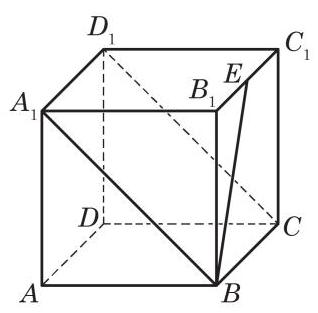
\includegraphics[max width=0.2\textwidth]{images/bo_d7fqvdc91nqc7381i9u0_103_1134_756_318_313_0.jpg}
\end{center}
\hspace*{3em} 

图 3-1-1

例 1 如图 3-1-1,在正方体 \({ABCD} - {A}_{1}{B}_{1}{C}_{1}{D}_{1}\) 中, \(E\) 为棱 \({B}_{1}{C}_{1}\) 上任意一点. 只考虑图上已作出线段所对应的向量, 分别写出:

(1) \(\overrightarrow{AB}\) 的相等向量， \(\overrightarrow{{A}_{1}B}\) 的负向量；

(2)用另外两个向量的和或差表示 \(\overrightarrow{B{B}_{1}}\) ；

(3)用三个或三个以上向量的和表示 \(\overrightarrow{BE}\) (举两个例子).

解(1)根据正方体棱与棱之间的关系， \(\overrightarrow{AB}\) 的相等向量有 \(\overrightarrow{{A}_{1}{B}_{1}}\text{ 、 }\overrightarrow{DC}\text{ 、 }\overrightarrow{{D}_{1}{C}_{1}},\overrightarrow{{A}_{1}B}\) 的负向量有 \(\overrightarrow{B{A}_{1}}\text{ 、 }\overrightarrow{C{D}_{1}}\) .

(2)此小题用“首尾规则”求解. 如果只在含 \(\overrightarrow{B{B}_{1}}\) 的三角形中考虑,有 \(\overrightarrow{B{B}_{1}} = \overrightarrow{B{A}_{1}} + \overrightarrow{{A}_{1}{B}_{1}},\overrightarrow{B{B}_{1}} = \overrightarrow{BE} + \overrightarrow{E{B}_{1}},\overrightarrow{B{B}_{1}} = \overrightarrow{B{A}_{1}} - \overrightarrow{{B}_{1}{A}_{1}}\) , \(\overrightarrow{B{B}_{1}} = \overrightarrow{BE} - \overrightarrow{{B}_{1}E}.\)

如果考虑 \(\overrightarrow{B{B}_{1}}\) 的相等向量所在的三角形,那么可以有更多的解答, 请同学们自行补出.

(3)此小题用“首尾规则”求解，有许多不同的答案，以下是两个例子:

\[
\overrightarrow{BE} = \overrightarrow{B{A}_{1}} + \overrightarrow{{A}_{1}{B}_{1}} + \overrightarrow{{B}_{1}E},
\]

\[
\overrightarrow{BE} = \overrightarrow{B{B}_{1}} + \overrightarrow{{B}_{1}{A}_{1}} + \overrightarrow{{A}_{1}{D}_{1}} + \overrightarrow{{D}_{1}{C}_{1}} + \overrightarrow{{C}_{1}E}\text{ . }
\]

\begin{center}
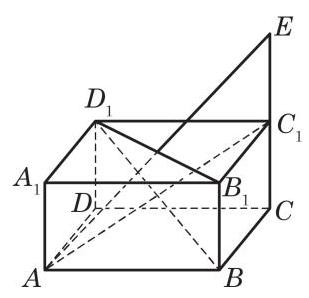
\includegraphics[max width=0.2\textwidth]{images/bo_d7fqvdc91nqc7381i9u0_103_1145_1745_309_298_0.jpg}
\end{center}
\hspace*{3em} 

图 3-1-2

例 2 如图 3-1-2,在长方体 \({ABCD} - {A}_{1}{B}_{1}{C}_{1}{D}_{1}\) 中,点 \(E\) 在棱 \(C{C}_{1}\) 的延长线上,且 \(\left| {{C}_{1}E}\right|  = \left| {C{C}_{1}}\right|\) . 设 \(\overrightarrow{A{A}_{1}} = \overrightarrow{a}\) , \(\overrightarrow{AB} = \overrightarrow{b},\overrightarrow{AD} = \overrightarrow{c}\) ,试用 \(\overrightarrow{a}\text{ 、 }\overrightarrow{b}\text{ 、 }\overrightarrow{c}\) 的线性组合表示下列向量:

(1) \(\overrightarrow{A{C}_{1}}\) ；(2) \(\overrightarrow{{D}_{1}{B}_{1}}\) ；(3) \(\overrightarrow{B{D}_{1}}\) ；(4) \(\overrightarrow{AE}\) .

解 (1) \(\overrightarrow{A{C}_{1}} = \overrightarrow{AB} + \overrightarrow{BC} + \overrightarrow{C{C}_{1}} = \overrightarrow{AB} + \overrightarrow{AD} + \overrightarrow{A{A}_{1}} = \overrightarrow{b} + \; \overrightarrow{c} + \overrightarrow{a}\) .

(2) \(\overrightarrow{{D}_{1}{B}_{1}} = \overrightarrow{{A}_{1}{B}_{1}} - \overrightarrow{{A}_{1}{D}_{1}} = \overrightarrow{AB} - \overrightarrow{AD} = \overrightarrow{b} - \overrightarrow{c}\) .

(3) \(\overrightarrow{B{D}_{1}} = \overrightarrow{BA} + \overrightarrow{A{A}_{1}} + \overrightarrow{{A}_{1}{D}_{1}} =  - \overrightarrow{AB} + \overrightarrow{A{A}_{1}} + \overrightarrow{AD} =  - \overrightarrow{b} + \; \overrightarrow{a} + \overrightarrow{c}\) .

(4) \(\overrightarrow{AE} = \overrightarrow{AB} + \overrightarrow{BC} + \overrightarrow{CE} = \overrightarrow{AB} + \overrightarrow{AD} + 2\overrightarrow{C{C}_{1}} = \overrightarrow{AB} + \overrightarrow{AD} + \; 2\overrightarrow{A{A}_{1}} = \overrightarrow{b} + \overrightarrow{c} + 2\overrightarrow{a}.\)

\section*{练习 3.1(1)}

\begin{center}
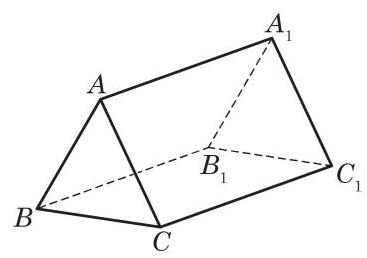
\includegraphics[max width=0.3\textwidth]{images/bo_d7fqvdc91nqc7381i9u0_104_1130_626_367_258_0.jpg}
\end{center}
\hspace*{3em} 

(第 2 题)

1. 空间中有异面向量的概念吗? 为什么?

2. 如图, 请在图中找出三个不共面的向量.

3. 化简下列算式:

(1)3(2 \(\overrightarrow{a} - \overrightarrow{b} - 4\overrightarrow{c}\) )—4( \(\overrightarrow{a} - 2\overrightarrow{b} + 3\overrightarrow{c}\) );

(2) \(\overrightarrow{OA} - \left\lbrack  {\overrightarrow{OB} - \left( {\overrightarrow{AB} - \overrightarrow{AC}}\right) }\right\rbrack\) .

向量的数量积对向量加法的分配律也涉及三个向量, 它们可能不共面，但是可以仿照平面向量中分配律的证明(见必修课程 8.2 节)给出空间向量情形的证明，见练习 3.1(2)第 2 题.

\begin{center}
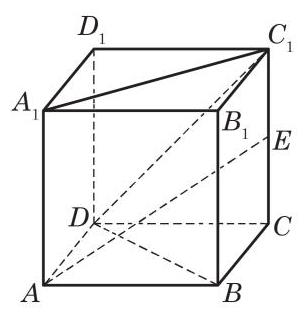
\includegraphics[max width=0.2\textwidth]{images/bo_d7fqvdc91nqc7381i9u0_104_190_1180_304_314_0.jpg}
\end{center}
\hspace*{3em} 

图 3-1-3

例 3 如图 3-1-3,已知正方体 \({ABCD} - {A}_{1}{B}_{1}{C}_{1}{D}_{1}\) 的棱长为 \(a,E\) 是棱 \(C{C}_{1}\) 的中点.

(1)求 \(\overrightarrow{D{D}_{1}} \cdot  \overrightarrow{D{C}_{1}}\) ；

(2)求 \(\overrightarrow{AE} \cdot  \overrightarrow{{C}_{1}{A}_{1}}\) ；

(3)求 \(\overrightarrow{AE}\) 与 \(\overrightarrow{{C}_{1}{A}_{1}}\) 的夹角的大小；

(4)判断 \(\overrightarrow{AE}\) 与 \(\overrightarrow{DB}\) 是否垂直.

解 (1) 由 \(\overrightarrow{D{D}_{1}} \bot  \overrightarrow{{D}_{1}{C}_{1}}\) 与 \(\left| \overrightarrow{D{D}_{1}}\right|  = \left| \overrightarrow{{D}_{1}{C}_{1}}\right|  = a\) ,得

\[
\left| \overrightarrow{D{C}_{1}}\right|  = \sqrt{{a}^{2} + {a}^{2}} = \sqrt{2}a.
\]

再根据向量数量积的定义, 得

\[
\overrightarrow{D{D}_{1}} \cdot  \overrightarrow{D{C}_{1}} = \left| \overrightarrow{D{D}_{1}}\right| \left| \overrightarrow{D{C}_{1}}\right| \cos \left\langle  {\overrightarrow{D{D}_{1}},\overrightarrow{D{C}_{1}}}\right\rangle
\]

\[
= a \cdot  \sqrt{2}a \cdot  \cos {45}^{ \circ  } = {a}^{2}.
\]

(2)因为

\[
\overrightarrow{AE} = \overrightarrow{AB} + \overrightarrow{BC} + \overrightarrow{CE} = \overrightarrow{AB} + \overrightarrow{BC} + \frac{1}{2}\overrightarrow{A{A}_{1}},
\]

\[
\overrightarrow{{C}_{1}{A}_{1}} = \overrightarrow{{C}_{1}{D}_{1}} + \overrightarrow{{D}_{1}{A}_{1}} =  - \overrightarrow{AB} - \overrightarrow{BC},
\]

并注意到 \(\overrightarrow{A{A}_{1}} \bot  \overrightarrow{AB},\overrightarrow{A{A}_{1}} \bot  \overrightarrow{BC},\overrightarrow{AB} \bot  \overrightarrow{BC}\) 以及 \(\left| {AB}\right|  = \left| {BC}\right|  = a\) ,

所以

\[
\overrightarrow{AE} \cdot  \overrightarrow{{C}_{1}{A}_{1}} = \left( {\overrightarrow{AB} + \overrightarrow{BC} + \frac{1}{2}\overrightarrow{A{A}_{1}}}\right)  \cdot  \left( {-\overrightarrow{AB} - \overrightarrow{BC}}\right)
\]

\[
=  - {\left( \overrightarrow{AB} + \overrightarrow{BC}\right) }^{2} - \frac{1}{2}\overrightarrow{A{A}_{1}} \cdot  \left( {\overrightarrow{AB} + \overrightarrow{BC}}\right)
\]

\[
=  - \overrightarrow{AB}{}^{2} - \overrightarrow{BC}{}^{2} =  - 2{a}^{2}\text{ . }
\]

(3)由(1)类似的方法，可得

\[
\left| \overrightarrow{{C}_{1}{A}_{1}}\right|  = \sqrt{2}a.
\]

又由 \(\overrightarrow{AB}\text{ 、 }\overrightarrow{BC}\) 与 \(\overrightarrow{A{A}_{1}}\) 两两互相垂直且模均为 \(a\) ,得

\[
\left| \overrightarrow{AE}\right|  = \sqrt{{\left( \overrightarrow{AB} + \overrightarrow{BC} + \frac{1}{2}\overrightarrow{A{A}_{1}}\right) }^{2}}
\]

\[
= \sqrt{{\left| \overrightarrow{AB}\right| }^{2} + {\left| \overrightarrow{BC}\right| }^{2} + \frac{1}{4}{\left| \overrightarrow{A{A}_{1}}\right| }^{2}} = \frac{3}{2}a.
\]

从而

\[
\cos \left\langle  {\overrightarrow{AE},\overrightarrow{{C}_{1}{A}_{1}}}\right\rangle   = \frac{\overrightarrow{AE} \cdot  \overrightarrow{{C}_{1}{A}_{1}}}{\left| \overrightarrow{AE}\right| \left| \overrightarrow{{C}_{1}{A}_{1}}\right| } = \frac{-2{a}^{2}}{\frac{3}{2}a \cdot  \sqrt{2}a}
\]

\[
=  - \frac{2\sqrt{2}}{3}\text{ . }
\]

所以

\[
\left\langle  {\overrightarrow{AE},\overrightarrow{{C}_{1}{A}_{1}}}\right\rangle   = \pi  - \arccos \frac{2\sqrt{2}}{3}.
\]

(4)由于 \(\overrightarrow{DB} = \overrightarrow{AB} - \overrightarrow{AD} = \overrightarrow{AB} - \overrightarrow{BC}\) ,且 \(\overrightarrow{AB} \bot  \overrightarrow{BC},\overrightarrow{A{A}_{1}} \bot \; \overrightarrow{AB},\overrightarrow{A{A}_{1}} \bot  \overrightarrow{BC}\) ,因此

\[
\overrightarrow{AE} \cdot  \overrightarrow{DB} = \left( {\overrightarrow{AB} + \overrightarrow{BC} + \frac{1}{2}\overrightarrow{A{A}_{1}}}\right)  \cdot  \left( {\overrightarrow{AB} - \overrightarrow{BC}}\right)
\]

\[
= {\left| \overrightarrow{AB}\right| }^{2} - {\left| \overrightarrow{BC}\right| }^{2} = {a}^{2} - {a}^{2} = 0,
\]

由此可知 \(\overrightarrow{AE} \bot  \overrightarrow{DB}\) .

平面向量平行的充要条件同样适用于空间向量, 即

空间中的向量 \(\overrightarrow{b}\) 与非零向量 \(\overrightarrow{a}\) 平行的充要条件是存在实数 \(\lambda\) ,使得 \(\overrightarrow{b} = \lambda \overrightarrow{a}\) .

平行向量也称为共线向量.

\HRule

例 3(3) 也可以用解三角形的方法求解.

例 3(4)可以用三垂线定理证明, 但三垂线定理是立体几何中有一定深度的内容, 本身的证明比较困难. 不过, 本章将用空间向量给出三垂线定理的一个简单证明 (本章 3.4 节例 1).

\HRule

\begin{center}
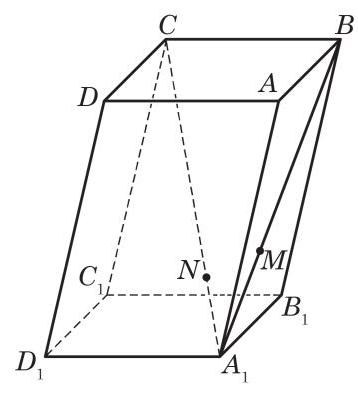
\includegraphics[max width=0.3\textwidth]{images/bo_d7fqvdc91nqc7381i9u0_106_177_240_358_393_0.jpg}
\end{center}
\hspace*{3em} 

图 3-1-4

例 4 底面是平行四边形的棱柱称为平行六面体, 其特点是六个面都是平行四边形, 且两两互相平行. 如图 3-1-4, 在平行六面体 \({ABCD} - {A}_{1}{B}_{1}{C}_{1}{D}_{1}\) 中,点 \(M\) 在对角线 \({A}_{1}B\) 上,且 \(\left| {{A}_{1}M}\right|  = \frac{1}{2}\left| {MB}\right|\) ,点 \(N\) 在对角线 \({A}_{1}C\) 上,且 \(\left| {{A}_{1}N}\right|  = \frac{1}{3}\left| {NC}\right|\) . 求证: \(M\text{ 、 }N\text{ 、 }{D}_{1}\) 三点共线.

证明 令 \(\overrightarrow{AB} = \overrightarrow{a},\overrightarrow{AD} = \overrightarrow{b},\overrightarrow{A{A}_{1}} = \overrightarrow{c}\) ,则

\[
\overrightarrow{{D}_{1}{A}_{1}} = \overrightarrow{DA} =  - \overrightarrow{b},
\]

\[
\overrightarrow{{A}_{1}B} = \overrightarrow{AB} - \overrightarrow{A{A}_{1}} = \overrightarrow{a} - \overrightarrow{c},
\]

\[
\overrightarrow{{A}_{1}M} = \frac{1}{3}\overrightarrow{{A}_{1}B} = \frac{1}{3}\left( {\overrightarrow{a} - \overrightarrow{c}}\right) ,
\]

所以, \(\overrightarrow{{D}_{1}M} = \overrightarrow{{D}_{1}{A}_{1}} + \overrightarrow{{A}_{1}M} =  - \overrightarrow{b} + \frac{1}{3}\left( {\overrightarrow{a} - \overrightarrow{c}}\right)  = \frac{1}{3}\left( {\overrightarrow{a} - 3\overrightarrow{b} - \overrightarrow{c}}\right)\) .

又因为

\[
\overrightarrow{{A}_{1}C} = \overrightarrow{{A}_{1}B} + \overrightarrow{BC} = \overrightarrow{{A}_{1}B} + \overrightarrow{AD} = \overrightarrow{a} - \overrightarrow{c} + \overrightarrow{b},
\]

\[
\overrightarrow{{A}_{1}N} = \frac{1}{4}\overrightarrow{{A}_{1}C} = \frac{1}{4}\left( {\overrightarrow{a} - \overrightarrow{c} + \overrightarrow{b}}\right) ,
\]

所以

\[
\overrightarrow{{D}_{1}N} = \overrightarrow{{D}_{1}{A}_{1}} + \overrightarrow{{A}_{1}N} =  - \overrightarrow{b} + \frac{1}{4}\left( {\overrightarrow{a} - \overrightarrow{c} + \overrightarrow{b}}\right)  = \frac{1}{4}\left( {\overrightarrow{a} - 3\overrightarrow{b} - \overrightarrow{c}}\right) .
\]

由此可知, \(\overrightarrow{{D}_{1}M} = \frac{4}{3}\overrightarrow{{D}_{1}N}\) ,所以 \(\overrightarrow{{D}_{1}M}//\overrightarrow{{D}_{1}N}\) .

因为点 \({D}_{1}\) 为 \(\overrightarrow{{D}_{1}M}\) 与 \(\overrightarrow{{D}_{1}N}\) 的公共起点,所以 \(M\text{ 、 }N\text{ 、 }{D}_{1}\) 三点共线.

\section*{练习 3.1(2)}

\begin{center}
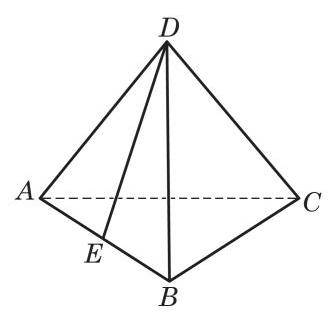
\includegraphics[max width=0.2\textwidth]{images/bo_d7fqvdc91nqc7381i9u0_106_1168_1705_330_314_0.jpg}
\end{center}
\hspace*{3em} 

(第 1 题)

1. 如图,棱长为 \(a\) 的正四面体 \({ABCD}\) 中, \(E\) 为棱 \({AB}\) 的中点. 求 \(\overrightarrow{DC} \cdot  \overrightarrow{DE}\) 与 \(\overrightarrow{BC} \cdot  \overrightarrow{DE}\) .

2. 设 \(\overrightarrow{a}\text{ 、 }\overrightarrow{b}\text{ 、 }\overrightarrow{c}\) 是三个空间向量,求证: \(\overrightarrow{a} \cdot  \left( {\overrightarrow{b} + \overrightarrow{c}}\right)  = \overrightarrow{a} \cdot  \overrightarrow{b} + \; \overrightarrow{a} \cdot  \overrightarrow{c}\)

\section*{习题 3.1}

\section*{A 组}

1. 在长方体 \({ABCD} - {A}^{\prime }{B}^{\prime }{C}^{\prime }{D}^{\prime }\) 中, \(\left| {AB}\right|  = 4,\left| {BC}\right|  = 3,\left| {A{A}^{\prime }}\right|  = 5\) . 写出:

(1)与 \(\overrightarrow{A{C}^{\prime }}\) 有相等模的向量；

(2) \(\overrightarrow{AB}\) 的相等向量；

(3)与 \(\overrightarrow{A{A}^{\prime }}\) 垂直的向量.

2. 如图，在直三棱柱 \({ABC} - {A}_{1}{B}_{1}{C}_{1}\) 中， \(\overrightarrow{CA} = \overrightarrow{a},\overrightarrow{CB} = \overrightarrow{b},\overrightarrow{C{C}_{1}} = \overrightarrow{c}\) . 将向量 \(\overrightarrow{{A}_{1}B}\) 表示为 \(\overrightarrow{a}\text{ 、 }\overrightarrow{b}\text{ 、 }\overrightarrow{c}\) 的线性组合.

\begin{center}
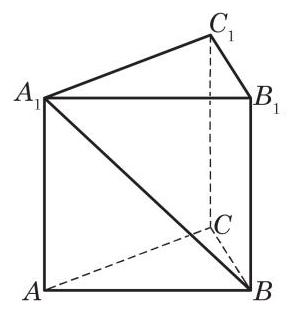
\includegraphics[max width=0.2\textwidth]{images/bo_d7fqvdc91nqc7381i9u0_107_402_915_290_311_0.jpg}
\end{center}
\hspace*{3em} 

(第 2 题)

\begin{center}
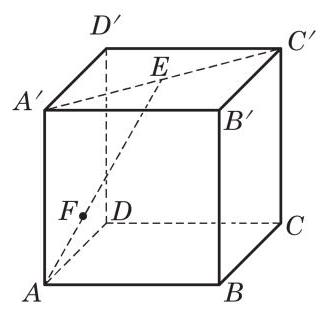
\includegraphics[max width=0.2\textwidth]{images/bo_d7fqvdc91nqc7381i9u0_107_876_912_320_312_0.jpg}
\end{center}
\hspace*{3em} 

(第 3 题)

3. 如图，在正方体 \({ABCD} - {A}^{\prime }{B}^{\prime }{C}^{\prime }{D}^{\prime }\) 中， \(E\) 是 \({A}^{\prime }{C}^{\prime }\) 的中点，点 \(F\) 在 \({AE}\) 上，且 \(\left| {AF}\right|  = \; \frac{1}{2}\left| {EF}\right|\) . 试用向量 \(\overrightarrow{A{A}^{\prime }}\) 、 \(\overrightarrow{AB}\) 与 \(\overrightarrow{AD}\) 的线性组合表示 \(\overrightarrow{AF}\) .

4. 已知 \(\overrightarrow{a}\bot \overrightarrow{b},\overrightarrow{c}\) 与 \(\overrightarrow{a}\text{ 、 }\overrightarrow{b}\) 的夹角都是 \({60}^{ \circ  }\) ,且 \(\left| \overrightarrow{a}\right|  = 1,\left| \overrightarrow{b}\right|  = 2,\left| \overrightarrow{c}\right|  = 3\) . 计算:

(1) \(\left( {{3\overrightarrow{a}} - 2\overrightarrow{b}}\right)  \cdot  \left( {\overrightarrow{b} - 3\overrightarrow{c}}\right)\) ；

(2) \(\left| {\overrightarrow{a} + 2\overrightarrow{b} - \overrightarrow{c}}\right|\) .

5. 已知空间四边形 \({ABCD}\) 中, \({AB} \bot  {CD},{AC} \bot  {BD}\) . 求证: \({AD} \bot  {BC}\) .

\begin{center}
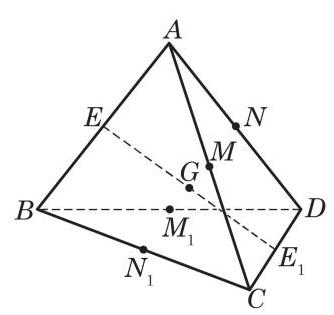
\includegraphics[max width=0.2\textwidth]{images/bo_d7fqvdc91nqc7381i9u0_107_1134_1737_334_315_0.jpg}
\end{center}
\hspace*{3em} 

(第 6 题)

6. 如图,在四面体 \({ABCD}\) 中, \(E\text{ 、 }M\text{ 、 }N\) 分别是棱 \({AB}\) 、 \({AC}\text{ 、 }{AD}\) 的中点, \({E}_{1}\text{ 、 }{M}_{1}\text{ 、 }{N}_{1}\) 分别是棱 \({CD}\text{ 、 }{BD}\text{ 、 }{BC}\) 的中点, \(G\) 是线段 \(E{E}_{1}\) 的中点. 试判断下列各组中的三点是否共线:

(1) \(G\) 、 \(M\) 、 \({M}_{1}\) ；

(2) \(G\) 、 \(N\) 、 \({N}_{1}\) .

\section*{B 组}

\begin{center}
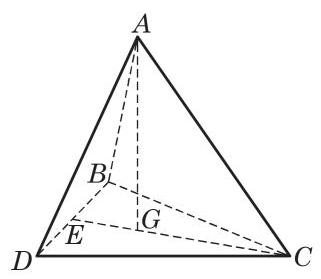
\includegraphics[max width=0.2\textwidth]{images/bo_d7fqvdc91nqc7381i9u0_108_1176_293_321_279_0.jpg}
\end{center}
\hspace*{3em} 

(第 1 题)

1. 如图, \(A\) 是 \(\bigtriangleup {BCD}\) 所在平面外一点, \(G\) 是 \(\bigtriangleup {BCD}\) 的重心. 求证: \(\overrightarrow{AG} = \frac{1}{3}\left( {\overrightarrow{AB} + \overrightarrow{AC} + \overrightarrow{AD}}\right)\) .

2. 如图,在三棱锥 \(D - {ABC}\) 中, \(\angle {DAC} = \angle {BAC} = {60}^{ \circ  }\) , \({AC} = 1,{AB} = 2,{AD} = 3.\)

(1)求 \(\overrightarrow{AC} \cdot  \overrightarrow{BD}\) ，并说明异面直线 \({AC}\) 与 \({BD}\) 所成的角 \(\theta\) 的大小在棱 \({BD}\) 长度增大时是怎样变化的；

(2)判断点 \(D\) 在平面 \({ABC}\) 上的射影是否可能在直线 \({BC}\) 上，给出你的结论并加以证明.

\begin{center}
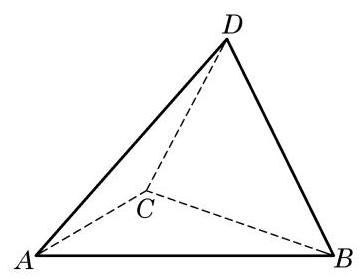
\includegraphics[max width=0.3\textwidth]{images/bo_d7fqvdc91nqc7381i9u0_108_353_837_361_279_0.jpg}
\end{center}
\hspace*{3em} 

(第 2 题)

\begin{center}
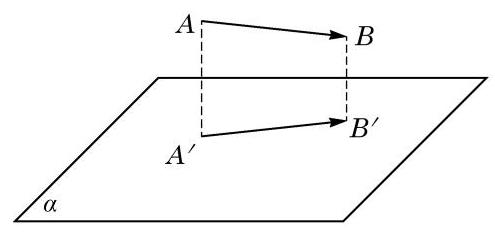
\includegraphics[max width=0.4\textwidth]{images/bo_d7fqvdc91nqc7381i9u0_108_827_870_495_233_0.jpg}
\end{center}
\hspace*{3em} 

(第 3 题)

3. 在空间中还可以讨论一个向量 \(\overrightarrow{AB}\) 在一个平面 \(\alpha\) 上的投影. 如图,若 \(\overrightarrow{a} = \overrightarrow{AB}\) ,点 \(A\) 与点 \(B\) 在平面 \(\alpha\) 上的投影分别是点 \({A}^{\prime }\) 与点 \({B}^{\prime }\) ,则 \(\overrightarrow{\alpha } = \overrightarrow{AB}\) 在平面 \(\alpha\) 上的投影就是向量 \(\overrightarrow{{A}^{\prime }{B}^{\prime }}\) . 现在给定向量 \(\overrightarrow{a}\) 、平面 \(\alpha\) 以及平面 \(\alpha\) 上的非零向量 \(\overrightarrow{b}\) . 设向量 \(\overrightarrow{a}\) 在平面 \(\alpha\) 上的投影是向量 \({\overrightarrow{a}}^{\prime }\) ,向量 \({\overrightarrow{a}}^{\prime }\) 在向量 \(\overrightarrow{b}\) 方向上的投影是向量 \({\overrightarrow{a}}^{\prime \prime }\) . 求证: 向量 \({\overrightarrow{a}}^{\prime \prime }\) 是向量 \(\overrightarrow{a}\) 在向量 \(\overrightarrow{b}\) 方向上的投影.

\section*{3.2 空间向量基本定理}

\section*{1 向量共面的充要条件}

我们在上一节中定义过的共面向量也可以用向量平行于平面的语言来刻画:如果一个向量所在的直线平行于一个平面， 那么称这个向量平行于这个平面. 一组向量共面是指它们平行于同一个平面, 也就是说, 它们通过平行移动可以放到同一平面上.

\begin{center}
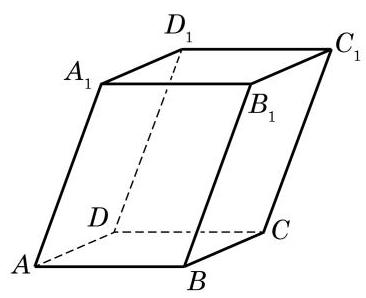
\includegraphics[max width=0.3\textwidth]{images/bo_d7fqvdc91nqc7381i9u0_109_1131_739_366_298_0.jpg}
\end{center}
\hspace*{3em} 

图 3-2-1

我们说过空间的任意两个向量总是共面的. 但是, 空间中的三个向量却不一定共面. 例如，图 3-2-1 所示的平行六面体中， 相交于一个顶点 \(A\) 的三条棱 \({AB}\text{ 、 }{AD}\) 与 \(A{A}_{1}\) 所对应的向量 \(\overrightarrow{AB}\) 、 \(\overrightarrow{AD}\) 与 \(\overrightarrow{A{A}_{1}}\) 就是不共面的.

因为两个向量的和是通过平行四边形或三角形 (都是平面图形)作出的, 所以两个向量的任何线性组合都与原来的两个向量共面. 反之, 如果给定两个互不平行的向量, 任意与这两个向量共面的向量都是这两个向量的线性组合. 这个结论是在给定的两个向量所在的平面上使用(见必修课程 8.1 节)平面向量基本定理得到的. 事实上, 平面向量基本定理在空间中应该叙述为如下的向量共面的充要条件. ?

向量共面的充要条件 如果 \(\overrightarrow{{e}_{1}}\) 与 \(\overrightarrow{{e}_{2}}\) 是两个不平行的向量,那么空间中的向量 \(\overrightarrow{a}\) 与 \(\overrightarrow{{e}_{1}}\text{ 、 }\overrightarrow{{e}_{2}}\) 共面的充要条件是,存在唯一的一对实数 \(\lambda\) 与 \(\mu\) ,使得

\[
\overrightarrow{a} = \lambda \overrightarrow{{e}_{1}} + \mu \overrightarrow{{e}_{2}}.
\]

\HRule

利用向量共面的充要条件, 如何用向量表达空间四点共面的充要条件? (对比必修课程 8.3 节的探究)

\HRule

\begin{center}
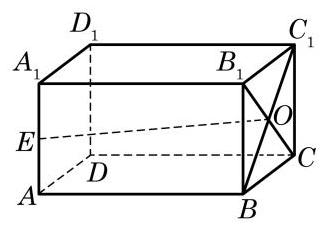
\includegraphics[max width=0.2\textwidth]{images/bo_d7fqvdc91nqc7381i9u0_109_1137_1865_322_228_0.jpg}
\end{center}
\hspace*{3em} 

图 3-2-2

例 1 如图 3-2-2,在长方体 \({ABCD} - {A}_{1}{B}_{1}{C}_{1}{D}_{1}\) 中, \(E\) 是棱 \(A{A}_{1}\) 的中点, \(O\) 是面对角线 \(B{C}_{1}\) 与 \({B}_{1}C\) 的交点. 试判断向量 \(\overrightarrow{EO}\) 与 \(\overrightarrow{AB}\) 、 \(\overrightarrow{AD}\) 是否共面.

解 因为

\[
\overrightarrow{EO} = \overrightarrow{EA} + \overrightarrow{AB} + \overrightarrow{BO},
\]

\[
\overrightarrow{BO} = \frac{1}{2}\left( {\overrightarrow{BC} + \overrightarrow{B{B}_{1}}}\right)  = \frac{1}{2}\left( {\overrightarrow{AD} + \overrightarrow{A{A}_{1}}}\right) ,
\]

所以

\[
\overrightarrow{EO} =  - \frac{1}{2}\overrightarrow{A{A}_{1}} + \overrightarrow{AB} + \frac{1}{2}\left( {\overrightarrow{AD} + \overrightarrow{A{A}_{1}}}\right)
\]

\[
= \overrightarrow{AB} + \frac{1}{2}\overrightarrow{AD},
\]

因此，向量 \(\overrightarrow{EO}\) 与 \(\overrightarrow{AB}\) 、 \(\overrightarrow{AD}\) 共面.

例 2 利用向量证明: 如果一条直线垂直于一个平面上的两条相交直线, 那么这条直线垂直于这个平面 (即垂直于这个平面中的任何直线).

Q

\HRule

例 2 是必修课程第 10 章中的直线与平面垂直的判定定理.

\HRule

\begin{center}
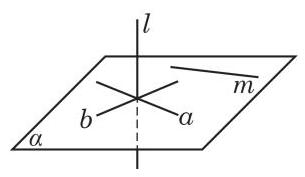
\includegraphics[max width=0.2\textwidth]{images/bo_d7fqvdc91nqc7381i9u0_110_182_975_305_177_0.jpg}
\end{center}
\hspace*{3em} 

图 3-2-3

已知 如图 3-2-3, \(a\text{ 、 }b\) 是平面 \(\alpha\) 上的两条相交直线,直线 \(l\) 满足 \(l \bot  a,l \bot  b\) .

求证 \(l \bot  \alpha\) .

证明 在平面 \(\alpha\) 上任意作直线 \(m\) ,并分别在直线 \(l\text{ 、 }a\text{ 、 }b\) 、 \(m\) 上取非零向量 \(\overrightarrow{l}\text{ 、 }\overrightarrow{a}\text{ 、 }\overrightarrow{b}\text{ 、 }\overrightarrow{m}\) .

因为直线 \(a\) 与 \(b\) 相交,所以向量 \(\overrightarrow{a}\text{ 、 }\overrightarrow{b}\) 不平行. 由向量共面的充要条件知, \(\overrightarrow{m}\) 是 \(\overrightarrow{a}\text{ 、 }\overrightarrow{b}\) 的线性组合,即

\[
\overrightarrow{m} = \lambda \overrightarrow{a} + \mu \overrightarrow{b}\left( {\lambda ,\mu  \in  \mathbf{R}}\right) .
\]

将上式两边与向量 \(\overrightarrow{l}\) 作数量积,由题意知 \(\overrightarrow{l} \cdot  \overrightarrow{a} = 0,\overrightarrow{l} \cdot  \overrightarrow{b} = 0\) , 所以

\[
\overrightarrow{l} \cdot  \overrightarrow{m} = \lambda \overrightarrow{l} \cdot  \overrightarrow{a} + \mu \overrightarrow{l} \cdot  \overrightarrow{b} = 0,
\]

从而 \(l \bot  m\) . 这说明直线 \(l\) 垂直于平面 \(\alpha\) 上的任意一条直线,所以 \(l \bot  \alpha\) .

\section*{2 空间向量基本定理}

已知平面上两个不共线向量的线性组合可以表示该平面上的所有向量. 是否可以做一个类推, 空间三个不共面向量的线性组合可以表示空间中的所有向量? 下面的定理对此给出了肯定的回答.

空间向量基本定理 如果 \(\overrightarrow{{e}_{1}}\text{ 、 }\overrightarrow{{e}_{2}}\) 与 \(\overrightarrow{{e}_{3}}\) 是不共面的向量, 那么对空间中任意一个向量 \(\overrightarrow{a}\) ,存在唯一的一组实数 \(\lambda \text{ 、 }\mu\) 与 \(\nu\) ,使得

\[
\overrightarrow{a} = \lambda \overrightarrow{{e}_{1}} + \mu \overrightarrow{{e}_{2}} + \nu \overrightarrow{{e}_{3}}.
\]

证明: 先证线性组合的存在性.

因为 \(\overrightarrow{{e}_{1}}\text{ 、 }\overrightarrow{{e}_{2}}\) 与 \(\overrightarrow{{e}_{3}}\) 不共面,所以它们都不是零向量. 我们还可以假设向量 \(\overrightarrow{a}\) 不与 \(\overrightarrow{{e}_{1}}\text{ 、 }\overrightarrow{{e}_{2}}\) 与 \(\overrightarrow{{e}_{3}}\) 中的任何两个向量共面,否则,由向量共面的充要条件就立即给出了我们所需要的线性组合.

如图 3-2-4,在空间任取一点 \(O\) ,作 \(\overrightarrow{OA} = \overrightarrow{{e}_{1}},\overrightarrow{OB} = \overrightarrow{{e}_{2}}\) , \(\overrightarrow{OC} = \overrightarrow{{e}_{3}},\overrightarrow{OP} = \overrightarrow{a}\) . \({OA}\) 与 \({OB}\) 是不重合的相交直线,它们确定了一个平面 \(\alpha ;{OC}\) 与 \({OP}\) 是不重合的相交直线,它们也确定一个平面 \(\beta\) . 平面 \(\alpha\) 与 \(\beta\) 不重合 (否则 \(\overrightarrow{{e}_{1}}\text{ 、 }\overrightarrow{{e}_{2}}\) 与 \(\overrightarrow{{e}_{3}}\) 共面),但有公共点 \(O\) ,所以它们有唯一的交线 \(l\) . 在 \(l\) 上任取一个非零向量 \(\overrightarrow{b}\) ,则 \(\overrightarrow{b}\) 与 \(\overrightarrow{{e}_{3}}\) 不共线.

\begin{center}
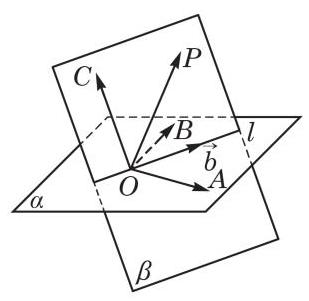
\includegraphics[max width=0.2\textwidth]{images/bo_d7fqvdc91nqc7381i9u0_111_1137_822_309_301_0.jpg}
\end{center}
\hspace*{3em} 

图 3-2-4

根据向量共面的充要条件，在平面 \(\alpha\) 上，向量 \(\overrightarrow{b}\) 是 \(\overrightarrow{OA}\) 与 \(\overrightarrow{OB}\) (即 \(\overrightarrow{{e}_{1}}\) 与 \(\overrightarrow{{e}_{2}}\) )的线性组合; 在平面 \(\beta\) 上,向量 \(\overrightarrow{a}\) 是向量 \(\overrightarrow{b}\) 与 \(\overrightarrow{OC}\) (即 \(\overrightarrow{{e}_{3}}\) ) 的线性组合. 于是,向量 \(\overrightarrow{a}\) 是向量 \(\overrightarrow{{e}_{1}}\text{ 、 }\overrightarrow{{e}_{2}}\) 与 \(\overrightarrow{{e}_{3}}\) 的线性组合.

再证线性组合的唯一性.

设 \(\overrightarrow{a} = \lambda \overrightarrow{{e}_{1}} + \mu \overrightarrow{{e}_{2}} + \nu \overrightarrow{{e}_{3}} = {\lambda }^{\prime }\overrightarrow{{e}_{1}} + {\mu }^{\prime }\overrightarrow{{e}_{2}} + {\nu }^{\prime }\overrightarrow{{e}_{3}}\) ,则

\[
\left( {\lambda  - {\lambda }^{\prime }}\right) \overrightarrow{{e}_{1}} + \left( {\mu  - {\mu }^{\prime }}\right) \overrightarrow{{e}_{2}} + \left( {\nu  - {\nu }^{\prime }}\right) \overrightarrow{{e}_{3}} = \overrightarrow{0}.
\]

如果此式左边三个系数中有一个 (比如 \(\lambda  - {\lambda }^{\prime }\) ) 非零,那么

\[
\overrightarrow{{e}_{1}} =  - \frac{\mu  - {\mu }^{\prime }}{\lambda  - {\lambda }^{\prime }}\overrightarrow{{e}_{2}} - \frac{\nu  - {\nu }^{\prime }}{\lambda  - {\lambda }^{\prime }}\overrightarrow{{e}_{3}},
\]

\begin{center}
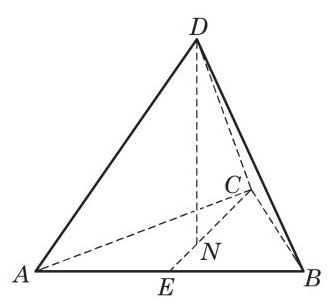
\includegraphics[max width=0.2\textwidth]{images/bo_d7fqvdc91nqc7381i9u0_111_1137_1698_329_303_0.jpg}
\end{center}
\hspace*{3em} 

图 3-2-5

这与 \(\overrightarrow{{e}_{1}}\text{ 、 }\overrightarrow{{e}_{2}}\) 与 \(\overrightarrow{{e}_{3}}\) 不共面矛盾. 所以三个系数必须全为零,则 \(\lambda  = \; {\lambda }^{\prime },\mu  = {\mu }^{\prime },\nu  = {\nu }^{\prime }\) . 所以,线性组合是唯一的.

例 3 如图 3-2-5,在正四面体 \({ABCD}\) 中, \(N\) 是面 \({ABC}\) 的中心.

(1)在此四面体的棱所对应的向量中找出两组各三个不共面的向量，并把其他棱对应的向量分别表示成这两组向量的线性组合 (互为负向量的不必另行表示), 要求第一组三个向量所在的棱有公共点, 第二组三个向量所在的棱没有公共点 (答案不唯一)；

(2)在(1)的条件下，把 \(\overrightarrow{DN}\) 也分别表示为这两组向量的线性组合. Q

\HRule

可以看出, 第一种选择有更好的对称性.

\HRule

解(1)第一组向量可选 \(\overrightarrow{DA} = \overrightarrow{a},\overrightarrow{DB} = \overrightarrow{b}\) 与 \(\overrightarrow{DC} = \overrightarrow{c}\) ,则

\[
\overrightarrow{AB} = \overrightarrow{b} - \overrightarrow{a},\overrightarrow{BC} = \overrightarrow{c} - \overrightarrow{b},\overrightarrow{CA} = \overrightarrow{a} - \overrightarrow{c}.
\]

第二组向量可选 \(\overrightarrow{DA} = \overrightarrow{a},\overrightarrow{DB} = \overrightarrow{b}\) 与 \(\overrightarrow{BC} = \overrightarrow{d}\) ,则

\[
\overrightarrow{AB} = \overrightarrow{b} - \overrightarrow{a},\overrightarrow{DC} = \overrightarrow{b} + \overrightarrow{d},\overrightarrow{CA} = \overrightarrow{a} - \overrightarrow{b} - \overrightarrow{d}.
\]

(2)如图 3-2-5，取 \(E\) 为 \({AB}\) 的中点，连接 \({CE}\) ，则点 \(N\) 在 \({CE}\) 上，且 \(\overrightarrow{CN} = \frac{2}{3}\overrightarrow{CE} = \frac{2}{3}\left( {\overrightarrow{CA} + \overrightarrow{AE}}\right)  = \frac{2}{3}\left( {\overrightarrow{CA} + \frac{1}{2}\overrightarrow{AB}}\right)\) ，所以

\[
\overrightarrow{DN} = \overrightarrow{DC} + \overrightarrow{CN} = \overrightarrow{DC} + \frac{2}{3}\left( {\overrightarrow{CA} + \frac{1}{2}\overrightarrow{AB}}\right)  = \overrightarrow{DC} + \frac{2}{3}\overrightarrow{CA} + \frac{1}{3}\overrightarrow{AB},
\]

分别代入 (1) 的结果, 化简得

\[
\overrightarrow{DN} = \frac{1}{3}\overrightarrow{a} + \frac{1}{3}\overrightarrow{b} + \frac{1}{3}\overrightarrow{c}\text{ 与 }\overrightarrow{DN} = \frac{1}{3}\overrightarrow{a} + \frac{2}{3}\overrightarrow{b} + \frac{1}{3}\overrightarrow{d}.
\]

\section*{练习 3.2}

1. 下列命题是否为真命题? 如果是, 请说明理由; 如果不是, 请举出反例.

(1)设 \(A\text{ 、 }B\text{ 、 }C\text{ 、 }D\) 是空间中的四个不同的点，直线 \({AB}\) 与 \({CD}\) 是异面直线，则向量 \(\overrightarrow{AB}\) 与 \(\overrightarrow{CD}\) 不共面;

(2)如果 \(\overrightarrow{a}\) 、 \(\overrightarrow{b}\) 是平面 \(\alpha\) 上的互不平行的向量，点 \(C\) 、 \(D\) 不在平面 \(\alpha\) 上，那么向量 \(\overrightarrow{CD}\) 与向量 \(\overrightarrow{a}\) 、 \(\overrightarrow{b}\) 不共面；

(3)如果 \(\overrightarrow{a}\) 、 \(\overrightarrow{b}\) 是平面 \(\alpha\) 上的互不平行的向量，点 \(C\) 在平面 \(\alpha\) 上，点 \(D\) 不在平面 \(\alpha\) 上， 那么向量 \(\overrightarrow{CD}\) 与向量 \(\overrightarrow{a}\) 、 \(\overrightarrow{b}\) 不共面.

\begin{center}
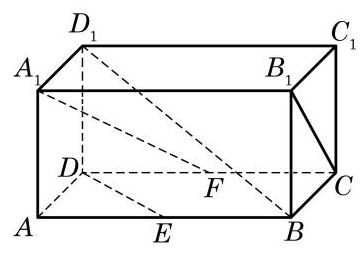
\includegraphics[max width=0.3\textwidth]{images/bo_d7fqvdc91nqc7381i9u0_112_1138_1594_363_253_0.jpg}
\end{center}
\hspace*{3em} 

(第 2 题)

2. 如图,在长方体 \({ABCD} - {A}_{1}{B}_{1}{C}_{1}{D}_{1}\) 中, \({AB} : A{A}_{1} : {AD} = \; 2 : 1 : 1,E\) 与 \(F\) 分别是棱 \({AB}\) 与 \({DC}\) 的中点. 设 \(\overrightarrow{A{A}_{1}} = \overrightarrow{a},\overrightarrow{AB} = \overrightarrow{b}\) , \(\overrightarrow{AD} = \overrightarrow{c}.\)

(1)用向量 \(\overrightarrow{a}\) 、 \(\overrightarrow{b}\) 、 \(\overrightarrow{c}\) 表示 \(\overrightarrow{B{D}_{1}}\) 、 \(\overrightarrow{{A}_{1}F}\) ；

(2)求 \(\overrightarrow{{A}_{1}F} \cdot  \overrightarrow{{B}_{1}C}\) ；

(3)判断 \(\overrightarrow{{A}_{1}F}\) 与 \(\overrightarrow{DE}\) 是否垂直.

\section*{习题 3.2}

\section*{A 组}

\begin{center}
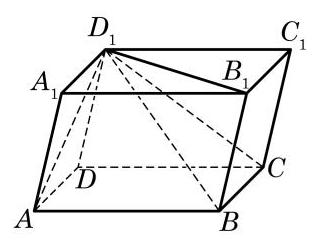
\includegraphics[max width=0.2\textwidth]{images/bo_d7fqvdc91nqc7381i9u0_113_1149_565_314_241_0.jpg}
\end{center}
\hspace*{3em} 

(第 1 题)

1. 如图,在平行六面体 \({ABCD} - {A}_{1}{B}_{1}{C}_{1}{D}_{1}\) 中,设 \(\overrightarrow{{D}_{1}A} = \overrightarrow{a}\) , \(\overrightarrow{{D}_{1}{B}_{1}} = \overrightarrow{b},\overrightarrow{{D}_{1}C} = \overrightarrow{c}\) . 试用 \(\overrightarrow{a}\text{ 、 }\overrightarrow{b}\text{ 、 }\overrightarrow{c}\) 表示 \(\overrightarrow{{D}_{1}B}\) .

2. 已知 \(\overrightarrow{a}\text{ 、 }\overrightarrow{b}\) 是空间的非零向量,分析 \(\overrightarrow{a} \cdot  \overrightarrow{b} = \left| \overrightarrow{a}\right|  \cdot  \left| \overrightarrow{b}\right|\) 与 \(\overrightarrow{a}//\overrightarrow{b}\) 的关系.

3. 在正方体 \({ABCD} - {A}^{\prime }{B}^{\prime }{C}^{\prime }{D}^{\prime }\) 中, \(E\) 是面 \({A}^{\prime }{B}^{\prime }{C}^{\prime }{D}^{\prime }\) 的中心. 求下列各式中实数 \(\lambda \text{ 、 }\mu \text{ 、 }\nu\) 的值:

(1) \(\overrightarrow{B{D}^{\prime }} = \lambda \overrightarrow{AD} + \mu \overrightarrow{AB} + \nu \overrightarrow{A{A}^{\prime }}\) ；

\begin{center}
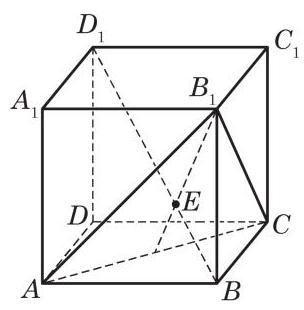
\includegraphics[max width=0.2\textwidth]{images/bo_d7fqvdc91nqc7381i9u0_113_1156_995_304_310_0.jpg}
\end{center}
\hspace*{3em} 

(第 4 题)

(2) \(\overrightarrow{AE} = \lambda \overrightarrow{AD} + \mu \overrightarrow{AB} + \nu \overrightarrow{A{A}^{\prime }}\) .

4. 如图,在棱长为 1 的正方体 \({ABCD} - {A}_{1}{B}_{1}{C}_{1}{D}_{1}\) 中, \(B{D}_{1}\) 交平面 \({AC}{B}_{1}\) 于点 \(E\) . 求证:

(1) \(B{D}_{1} \bot\) 平面 \({AC}{B}_{1}\) ；

(2) \(\left| {BE}\right|  = \frac{1}{2}\left| {E{D}_{1}}\right|\) .

\section*{B 组}

1. 在平面上有如下命题: “若 \(O\) 为直线 \({AB}\) 外的一点,则点 \(P\) 在直线 \({AB}\) 上的充要条件是:存在实数 \(\lambda\) 、 \(\mu\) ，满足 \(\overrightarrow{OP} = \lambda \overrightarrow{OA} + \mu \overrightarrow{OB}\) ，且 \(\lambda  + \mu  = 1\) . ”类比此命题，给出空间某点在某一平面上的充要条件并加以证明.

\begin{center}
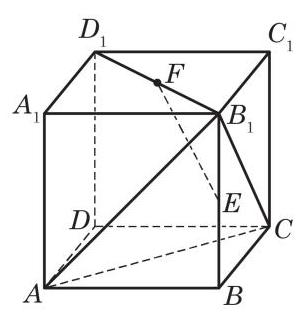
\includegraphics[max width=0.2\textwidth]{images/bo_d7fqvdc91nqc7381i9u0_113_1154_1658_300_315_0.jpg}
\end{center}
\hspace*{3em} 

(第 2 题)

2. 如图,在正方体 \({ABCD} - {A}_{1}{B}_{1}{C}_{1}{D}_{1}\) 中, \(E\text{ 、 }F\) 分别是 \(B{B}_{1}\text{ 、 }{D}_{1}{B}_{1}\) 的中点. 求证: \({EF} \bot\) 平面 \({B}_{1}{AC}\) .

3. 在棱长为 1 的正方体 \({ABCD} - {A}_{1}{B}_{1}{C}_{1}{D}_{1}\) 中, \(E\text{ 、 }F\) 分别是 \(D{D}_{1}\text{ 、 }{DB}\) 的中点,点 \(G\) 在棱 \({CD}\) 上, \(\left| {CG}\right|  = \frac{1}{4}\left| {CD}\right| ,H\) 是 \({C}_{1}G\) 的中点.

(1)求证: \({EF}\bot {B}_{1}C\) ；

(2)求 \({EF}\) 与 \({C}_{1}G\) 所成角的余弦值；

(3)求线段 \({FH}\) 的长.

\section*{3.3 空间向量的坐标表示}

平面向量的坐标表示使得向量的运算可以转化为向量坐标的代数运算, 带来了很大的方便. 空间向量也可以类似处理. 但为此要先建立空间直角坐标系.

\section*{1 空间直角坐标系}

如图 3-3-1, 在正方体中, 总可以找到从一个顶点出发的三条两两互相垂直的棱,如 \({AB}\text{ 、 }{AD}\) 与 \(A{A}_{1}\) . 受此启示,从空间一点 \(O\) 出发，可以作三条两两互相垂直的坐标轴，建立空间直角坐标系 \(O - {xyz}\) (图 3-3-2).

\begin{center}
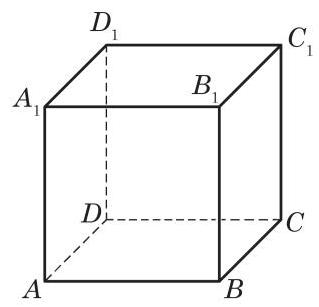
\includegraphics[max width=0.2\textwidth]{images/bo_d7fqvdc91nqc7381i9u0_114_647_1199_319_307_0.jpg}
\end{center}
\hspace*{3em} 

图 3-3-1

\begin{center}
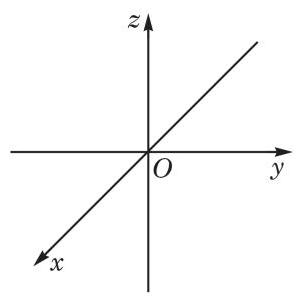
\includegraphics[max width=0.2\textwidth]{images/bo_d7fqvdc91nqc7381i9u0_114_1095_1208_298_298_0.jpg}
\end{center}
\hspace*{3em} 

图 3-3-2

点 \(O\) 叫做坐标原点,三条坐标轴分别是横轴 (即 \(x\) 轴)、纵轴 (即 \(y\) 轴) 与竖轴 (即 \(z\) 轴). 我们约定坐标系采用右手制,即右手翘起拇指、其他四指握拳做“点赞”状，当四指所指的方向是 \(x\) 轴正方向到 \(y\) 轴正方向的旋转方向时,拇指所指为 \(z\) 轴正方向 (图 3-3-3). 通过每两个坐标轴的平面叫坐标平面, 分别称为 \({xOy}\) 平面, \({yOz}\) 平面与 \({zOx}\) 平面. 三个坐标平面把空间划分成八个部分，每个部分称为一个卦限(octant)(图 3-3-4).

\begin{center}
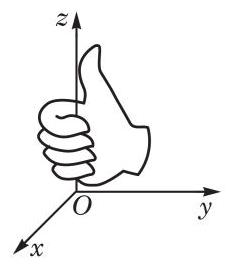
\includegraphics[max width=0.2\textwidth]{images/bo_d7fqvdc91nqc7381i9u0_115_303_238_226_264_0.jpg}
\end{center}
\hspace*{3em} 

图 3-3-3

\begin{center}
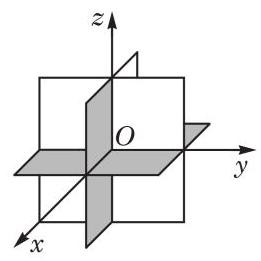
\includegraphics[max width=0.2\textwidth]{images/bo_d7fqvdc91nqc7381i9u0_115_706_237_261_261_0.jpg}
\end{center}
\hspace*{3em} 

图 3-3-4

给定空间一点 \(P\) ,如图 3-3-5,过点 \(P\) 分别作与坐标平面 \({yOz}\text{ 、 }{zOx}\) 与 \({xOy}\) 平行的平面,与坐标平面一起围出一个长方体，所作的三个平面与 \(x\) 轴、 \(y\) 轴、 \(z\) 轴的交点 \(A\text{ 、 }B\text{ 、 }C\) (它们都是上述长方体的顶点)在轴上的坐标,给出了点 \(P\) 的坐标 \((x,y\) , \(z)\) ,其中 \(x\text{ 、 }y\) 与 \(z\) 分别称为点 \(P\) 的横坐标、纵坐标与竖坐标.

\begin{center}
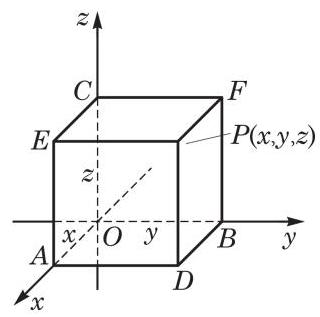
\includegraphics[max width=0.2\textwidth]{images/bo_d7fqvdc91nqc7381i9u0_115_479_886_320_317_0.jpg}
\end{center}
\hspace*{3em} 

图 3-3-5

有了空间直角坐标系, 空间中的点与实数的有序三元组就建立了一一对应.

例 1 在空间直角坐标系 \(O - {xyz}\) 中给定点 \(P\left( {7,6,4}\right)\) ,求该点关于坐标平面 \({xOy}\) 的对称点 \({P}^{\prime }\) 的坐标.

解 如图 3-3-6,过点 \(P\) 分别作与三个坐标平面平行的平面,与坐标平面一起围成了长方体 \({OADB} - {CEPF}\) ,根据点 \(P\) 的坐标知道 \(A\text{ 、 }B\text{ 、 }C\) 三点在轴上的坐标分别是 \(7\text{ 、 }6\text{ 、 }4\) .

\begin{center}
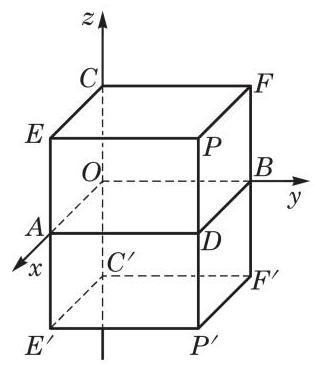
\includegraphics[max width=0.2\textwidth]{images/bo_d7fqvdc91nqc7381i9u0_115_468_1740_315_365_0.jpg}
\end{center}
\hspace*{3em} 

图 3-3-6

\HRule

不难看出, \(A\) 、 \(B\text{ 、 }C\) 分别是从点 \(P\) 所作的坐标轴的垂线 \({PA}\text{ 、 }{PB}\text{ 、 }{PC}\) (图上未画出)的垂足.

\HRule

因为 \({PD} \bot\) 平面 \({xOy}\) ,所以点 \(P\) 关于坐标平面 \({xOy}\) 的对称点 \({P}^{\prime }\) 在 \({PD}\) 延长线上,并使 \(\left| {PD}\right|  = \left| {D{P}^{\prime }}\right|\) .

为了求出点 \({P}^{\prime }\) 的坐标,把长方体 \({OADB}\) -CEPF 关于坐标平面 \({xOy}\) 作对称: 分别作 \({EA}\text{ 、 }{CO}\text{ 、 }{FB}\) 的延长线到点 \({E}^{\prime }\text{ 、 }{C}^{\prime }\text{ 、 }{F}^{\prime }\) ,使 \(\left| {EA}\right|  = \left| {A{E}^{\prime }}\right| ,\left| {CO}\right|  = \left| {O{C}^{\prime }}\right| ,\left| {FB}\right|  = \left| {B{F}^{\prime }}\right|\) ,则得到长方体 \({OADB} - {CEPF}\) 关于坐标平面 \({xOy}\) 的对称长方体 \({OADB} - {C}^{\prime }{E}^{\prime }{P}^{\prime }{F}^{\prime }\) ， 可见点 \({P}^{\prime }\) 的坐标由点 \(A\) 、 \(B\) 、 \({C}^{\prime }\) 在轴上的坐标给出. 又因为点 \({C}^{\prime }\) 在 \({Oz}\) 轴上的坐标与点 \(C\) 在 \({Oz}\) 轴上的坐标互为相反数,所以点 \(A\) 、 \(B\text{ 、 }{C}^{\prime }\) 在轴上的坐标分别是 \(7\text{ 、 }6\text{ 、 } - 4\) ,即点 \({P}^{\prime }\) 的坐标是 \(\left( {7,6, - 4}\right)\) .

\section*{2 空间向量的坐标表示}

模仿平面的情况,设 \(\overrightarrow{i}\text{ 、 }\overrightarrow{j}\text{ 、 }\overrightarrow{k}\) 分别是 \(x\) 轴、 \(y\) 轴、 \(z\) 轴正方向的单位向量. 由于三个坐标轴两两互相垂直, 因此这些向量之间的数量积为

\[
{\overrightarrow{i}}^{2} = {\overrightarrow{j}}^{2} = {\overrightarrow{k}}^{2} = 1,\overrightarrow{i} \cdot  \overrightarrow{j} = \overrightarrow{j} \cdot  \overrightarrow{k} = \overrightarrow{k} \cdot  \overrightarrow{i} = 0.
\]

给定任意一个向量 \(\overrightarrow{p}\) . 我们先通过平移把 \(\overrightarrow{p}\) 的起点放到坐标原点 \(O\) ,这时得到的向量 \(\overrightarrow{OP}\) 称为 \(\overrightarrow{p}\) 的位置向量. 设 \(\overrightarrow{OP}\) 的终点坐标是 \(P\left( {x,y,z}\right)\) ,则直接记 \(\overrightarrow{p} = \left( {x,y,z}\right)\) ,并称向量的这种表示法为它的坐标表示.

从图 3-3-5 可以看出, \(\overrightarrow{OP} = \overrightarrow{OA} + \overrightarrow{AD} + \overrightarrow{DP} = \overrightarrow{OA} + \overrightarrow{OB} + \overrightarrow{OC}\) , 而根据点的坐标的定义， \(\overrightarrow{OA} = x\overrightarrow{i},\overrightarrow{OB} = y\overrightarrow{j},\overrightarrow{OC} = z\overrightarrow{k}\) ，所以 \(\overrightarrow{p} = \left( {x,y,z}\right)\) 的实际含义是

\[
\overrightarrow{p} = x\overrightarrow{i} + y\overrightarrow{j} + z\overrightarrow{k}.
\]

有了这个表达式, 就可以像平面向量那样推知: 如果 \(\left( {{x}_{1},{y}_{1},{z}_{1}}\right) \text{ 、 }\left( {{x}_{2},{y}_{2},{z}_{2}}\right)\) 与 \(\left( {x,y,z}\right)\) 是坐标表示的向量, \(\lambda\) 是实数, 那么

\[
\left( {{x}_{1},{y}_{1},{z}_{1}}\right)  \pm  \left( {{x}_{2},{y}_{2},{z}_{2}}\right)  = \left( {{x}_{1} \pm  {x}_{2},{y}_{1} \pm  {y}_{2},{z}_{1} \pm  {z}_{2}}\right) ,
\]

\[
\lambda \left( {x,y,z}\right)  = \left( {{\lambda x},{\lambda y},{\lambda z}}\right) .
\]

这说明: 把向量用坐标表示后, 两个向量相加 (减), 等于把它们的对应坐标相加(减); 一个实数乘一个向量, 等于把这个实数乘它的坐标.

一个向量 \(\overrightarrow{p} = \left( {x,y,z}\right)\) 的模就是它的位置向量 \(\overrightarrow{OP}\) 的终点 \(P\) 与坐标原点 \(O\) 的距离,所以

\[
\left| \overrightarrow{OP}\right|  = \left| \left( {x,y,z}\right) \right|  = \sqrt{{x}^{2} + {y}^{2} + {z}^{2}}.
\]

如果向量不是由位置向量给出, 也可以不通过位置向量得到此向量的坐标表示: 设有空间任意两点 \(P\left( {{x}_{1},{y}_{1},{z}_{1}}\right)\) 与 \(Q\left( {{x}_{2},{y}_{2},{z}_{2}}\right)\) ,则

\[
\overrightarrow{PQ} = \overrightarrow{OQ} - \overrightarrow{OP}
\]

\[
= \left( {{x}_{2},{y}_{2},{z}_{2}}\right)  - \left( {{x}_{1},{y}_{1},{z}_{1}}\right)
\]

\[
= \left( {{x}_{2} - {x}_{1},{y}_{2} - {y}_{1},{z}_{2} - {z}_{1}}\right) \text{ . }
\]

即, 一个向量的坐标等于这个向量的终点坐标减去它的起点坐标.

有了上面两个公式,空间任意两点 \(P\left( {{x}_{1},{y}_{1},{z}_{1}}\right)\) 与 \(Q\left( {{x}_{2},{y}_{2},{z}_{2}}\right)\) 的距离就很容易求出了,因为这两点的距离 \(\left| {PQ}\right|\) 等于向量 \(\overrightarrow{PQ} = \left( {{x}_{2} - {x}_{1},{y}_{2} - {y}_{1},{z}_{2} - {z}_{1}}\right)\) 的模 \(\left| \overrightarrow{PQ}\right|\) . 由此得到

\[
\left| \overrightarrow{PQ}\right|  = \sqrt{{\left( {x}_{2} - {x}_{1}\right) }^{2} + {\left( {y}_{2} - {y}_{1}\right) }^{2} + {\left( {z}_{2} - {z}_{1}\right) }^{2}}.
\]

最后, 我们看两个空间向量的数量积如何用坐标表示.

给定两个向量 \(\overrightarrow{a} = \left( {{x}_{1},{y}_{1},{z}_{1}}\right)\) 与 \(\overrightarrow{b} = \left( {{x}_{2},{y}_{2},{z}_{2}}\right)\) ,把它们写成坐标轴正方向的单位向量的线性组合,就有 \(\overrightarrow{a} = {x}_{1}\overrightarrow{i} + {y}_{1}\overrightarrow{j} + \; {z}_{1}\overrightarrow{k}\) 与 \(\overrightarrow{b} = {x}_{2}\overrightarrow{i} + {y}_{2}\overrightarrow{j} + {z}_{2}\overrightarrow{k}\) ,于是

\[
\overrightarrow{a} \cdot  \overrightarrow{b} = \left( {{x}_{1}\overrightarrow{i} + {y}_{1}\overrightarrow{j} + {z}_{1}\overrightarrow{k}}\right)  \cdot  \left( {{x}_{2}\overrightarrow{i} + {y}_{2}\overrightarrow{j} + {z}_{2}\overrightarrow{k}}\right) .
\]

对上式用分配律展开计算,并注意到 \(\overrightarrow{i}\text{ 、 }\overrightarrow{j}\text{ 、 }\overrightarrow{k}\) 是两两互相垂直的向量,且 \({\overrightarrow{i}}^{2} = {\overrightarrow{j}}^{2} = {\overrightarrow{k}}^{2} = 1\) ,所以

\[
\overrightarrow{a} \cdot  \overrightarrow{b} = {x}_{1}{x}_{2}{\overrightarrow{i}}^{2} + {y}_{1}{y}_{2}{\overrightarrow{j}}^{2} + {z}_{1}{z}_{2}{\overrightarrow{k}}^{2} = {x}_{1}{x}_{2} + {y}_{1}{y}_{2} + {z}_{1}{z}_{2}.
\]

这就是我们所需要的两向量数量积公式

\[
\left( {{x}_{1},{y}_{1},{z}_{1}}\right)  \cdot  \left( {{x}_{2},{y}_{2},{z}_{2}}\right)  = {x}_{1}{x}_{2} + {y}_{1}{y}_{2} + {z}_{1}{z}_{2}.
\]

两个非零向量 \(\overrightarrow{a} = \left( {{x}_{1},{y}_{1},{z}_{1}}\right)\) 与 \(\overrightarrow{b} = \left( {{x}_{2},{y}_{2},{z}_{2}}\right)\) 夹角的余弦公式是

\[
\cos \langle \overrightarrow{a},\overrightarrow{b}\rangle  = \frac{{x}_{1}{x}_{2} + {y}_{1}{y}_{2} + {z}_{1}{z}_{2}}{\sqrt{{x}_{1}^{2} + {y}_{1}^{2} + {z}_{1}^{2}}\sqrt{{x}_{2}^{2} + {y}_{2}^{2} + {z}_{2}^{2}}}.
\]

从两向量夹角的余弦公式和两向量平行的充要条件可分别得到两个非零向量垂直与平行的充要条件:

\(\overrightarrow{a} \bot  \overrightarrow{b} \Leftrightarrow  {x}_{1}{x}_{2} + {y}_{1}{y}_{2} + {z}_{1}{z}_{2} = 0;\)

\(\overrightarrow{a}//\overrightarrow{b} \Leftrightarrow\) 存在 \(\lambda  \in  \mathbf{R}\) ,使得 \({x}_{1} = \lambda {x}_{2},{y}_{1} = \lambda {y}_{2},{z}_{1} = \lambda {z}_{2}\) .

解(1)以点 \(A\) 为坐标原点，分别以射线 \({AB}\) 、 \({AD}\) 、 \(A{A}_{1}\) 为 \(x\) 轴、 \(y\) 轴、 \(z\) 轴的正半轴,建立空间直角坐标系. 设正方体的棱长为 \(a\) ,可得有关点的坐标分别为 \(B\left( {a,0,0}\right) \text{ 、 }D\left( {0,a,0}\right)\) 、 \(C\left( {a,a,0}\right) \text{ 、 }{A}_{1}\left( {0,0,a}\right)\) ,从而 \(\overrightarrow{CA} = \left( {-a, - a,0}\right) ,\overrightarrow{C{A}_{1}} = \; \left( {-a, - a,a}\right)\) . 于是

\begin{center}
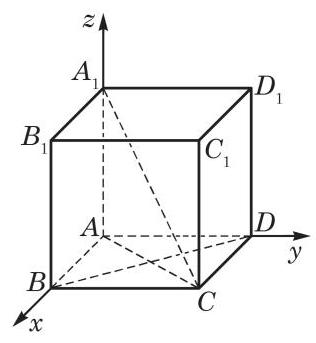
\includegraphics[max width=0.2\textwidth]{images/bo_d7fqvdc91nqc7381i9u0_118_187_743_316_343_0.jpg}
\end{center}
\hspace*{3em} 

图 3-3-7

例 2 如图 3-3-7,给定正方体 \({ABCD} - {A}_{1}{B}_{1}{C}_{1}{D}_{1}\) .

(1)求对角线 \(C{A}_{1}\) 与 \({CA}\) 所成角的余弦值；

(2)求证: \(C{A}_{1} \bot  {BD}\) .

\[
\cos \left\langle  {\overrightarrow{C{A}_{1}},\overrightarrow{CA}}\right\rangle   = \frac{\overrightarrow{C{A}_{1}} \cdot  \overrightarrow{CA}}{\left| \overrightarrow{C{A}_{1}}\right| \left| \overrightarrow{CA}\right| } = \frac{{a}^{2} + {a}^{2}}{\sqrt{{a}^{2} + {a}^{2}}\sqrt{{a}^{2} + {a}^{2} + {a}^{2}}} = \frac{2}{\sqrt{6}} = \frac{\sqrt{6}}{3}.
\]

所以,对角线 \(C{A}_{1}\) 与 \({CA}\) 所成角的余弦值为 \(\frac{\sqrt{6}}{3}\) .

(2)证明:由 \(\overrightarrow{C{A}_{1}} = \left( {-a, - a,a}\right) ,\overrightarrow{BD} = \left( {-a,a,0}\right)\) ，得

\[
\overrightarrow{C{A}_{1}} \cdot  \overrightarrow{BD} = {\left( -a\right) }^{2} + \left( {-a}\right) a + 0 = 0.
\]

所以, \(C{A}_{1} \bot  {BD}\) .

\section*{练习 3.3}

1. 讨论满足下列条件的点 \(P\) 的坐标 \(\left( {x,y,z}\right)\) 的特征:

(1)点 \(P\) 在坐标平面上; (2)点 \(P\) 在坐标轴上.

2. 求向量 \(\overrightarrow{a} = \left( {0,1,0}\right)\) 与 \(\overrightarrow{b} = \left( {1, - 1,0}\right)\) 的夹角的大小.

3. 已知向量 \(\overrightarrow{a} = \left( {-m,1,3}\right)\) 平行于向量 \(\overrightarrow{b} = \left( {2,n,1}\right)\) ，求 \(m\text{ 、 }n\) .

\section*{习题 3.3}

\section*{A 组}

1. 已知长方体 \({ABCD} - {A}_{1}{B}_{1}{C}_{1}{D}_{1}\) 的棱长 \(\left| {AB}\right|  = {14},\left| {AD}\right|  = 6,\left| {A{A}_{1}}\right|  = {10}\) ,以这个长方体的顶点 \(A\) 为坐标原点,分别以射线 \({AB}\text{ 、 }{AD}\text{ 、 }A{A}_{1}\) 为 \(x\) 轴、 \(y\) 轴、 \(z\) 轴的正半轴, 建立空间直角坐标系. 求长方体各顶点的坐标.

2. 已知 \({PA}\) 垂直于正方形 \({ABCD}\) 所在的平面, \(M\text{ 、 }N\) 分别是 \({AB}\text{ 、 }{PC}\) 的中点,且 \(\left| {PA}\right|  = \left| {AD}\right|\) ,分别以射线 \({AB}\text{ 、 }{AD}\text{ 、 }{AP}\) 为 \(x\) 轴、 \(y\) 轴、 \(z\) 轴的正半轴,建立空间直角坐标系. 求向量 \(\overrightarrow{MN}\text{ 、 }\overrightarrow{DC}\) 的坐标表示.

3. 已知 \(\overrightarrow{a} = \overrightarrow{i} + \overrightarrow{j} - 4\overrightarrow{k},\overrightarrow{b} = \overrightarrow{i} - 2\overrightarrow{j} + 2\overrightarrow{k}\) . 求:

(1)向量 \(\overrightarrow{a}\) 与 \(\overrightarrow{b}\) 的夹角的大小；

(2)向量 \(\overrightarrow{a}\) 与 \(\overrightarrow{b}\) 所在直线的夹角的大小.

4. 已知平行四边形 \({ABCD}\) 中的三个顶点的坐标分别为 \(A\left( {1,2,3}\right) \text{ 、 }B\left( {2, - 1,5}\right)\) 与 \(C\left( {3,2, - 5}\right)\) ,求顶点 \(D\) 的坐标.

5. 设 \(\overrightarrow{a} = \left( {{a}_{1},{a}_{2},{a}_{3}}\right) ,\overrightarrow{b} = \left( {{b}_{1},{b}_{2},{b}_{3}}\right)\) ,且 \(\overrightarrow{a} \neq  \overrightarrow{b}\) . 记 \(\left| {\overrightarrow{a} - \overrightarrow{b}}\right|  = m\) ,求 \(\overrightarrow{a} - \overrightarrow{b}\) 与 \(x\) 轴正方向向量夹角的余弦值.

\section*{B 组}

1. 在 \(\bigtriangleup {ABC}\) 中,已知 \(\overrightarrow{AB} = \left( {2,4,0}\right) ,\overrightarrow{BC} = \left( {-1,3,0}\right)\) . 求 \(\angle {ABC}\) 的大小.

2. 给定空间三点 \(A\left( {0,2,3}\right) \text{ 、 }B\left( {-2,1,6}\right) \text{ 、 }C\left( {1, - 1,5}\right)\) .

(1)求以向量 \(\overrightarrow{AB}\) 、 \(\overrightarrow{AC}\) 为一组邻边的平行四边形的面积 \(S\) ；

(2)若向量 \(\overrightarrow{a}\) 与向量 \(\overrightarrow{AB}\) 、 \(\overrightarrow{AC}\) 都垂直，且 \(\left| \overrightarrow{a}\right|  = \sqrt{3}\) ，求向量 \(\overrightarrow{a}\) 的坐标.

\begin{center}
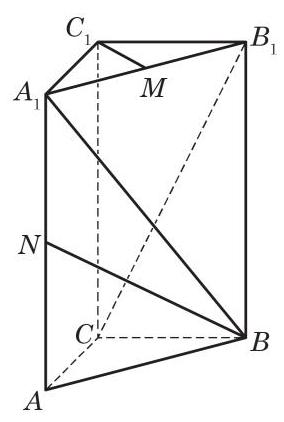
\includegraphics[max width=0.2\textwidth]{images/bo_d7fqvdc91nqc7381i9u0_119_1186_1675_284_422_0.jpg}
\end{center}
\hspace*{3em} 

(第 3 题)

3. 如图,在直三棱柱 \({ABC} - {A}_{1}{B}_{1}{C}_{1}\) 中, \(\left| {CA}\right|  = \left| {CB}\right|  = 1\) , \(\angle {BCA} = {90}^{ \circ  },\left| {A{A}_{1}}\right|  = 2,M\text{ 、 }N\) 分别是 \({A}_{1}{B}_{1}\text{ 、 }{A}_{1}A\) 的中点. 建立适当的空间直角坐标系, 解决如下问题:

(1)求 \(\overrightarrow{BN}\) 的模；

(2)求 \(\cos \left\langle  {\overrightarrow{B{A}_{1}},\overrightarrow{C{B}_{1}}}\right\rangle\) ；

(3)求证: \({A}_{1}B \bot  {C}_{1}M\) .

\section*{3.4 空间向量在立体几何中的应用}

空间向量常常可为解决立体几何中的有关问题提供简捷方便的方法. 在本章 3.2 节的例 2 中就非常方便地利用向量证明了直线与平面垂直的判定定理.

本节继续介绍空间向量在立体几何中的一些应用. 如下一些与直线和平面相关的向量是很重要的.

直线的方向向量: 与直线平行的任何非零向量.

平面的法向量: 垂直于平面的任何非零向量.

用向量方法解决有关直线和平面的问题, 一般先把相应的问题化为关于上述这些向量的问题然后加以解决. 建立一个适当的空间直角坐标系常常是有效的辅助手段, 特别是在需要数值求解的问题上.

\section*{1 判断空间直线、平面的位置关系}

下面的结论是显然的:

两条直线平行的充要条件是它们的方向向量平行; 两条直线垂直的充要条件是它们的方向向量垂直.

这样, 就把直线间的平行或垂直关系化为向量的平行或垂直关系. 我们给出一个“简单”的例子——三垂线定理的向量证明， 它的关键就是把直线垂直问题化为向量垂直问题.

\begin{center}
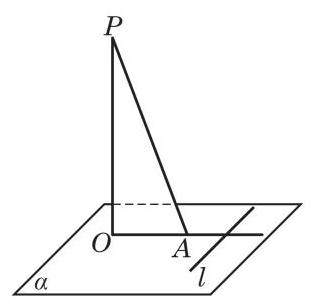
\includegraphics[max width=0.2\textwidth]{images/bo_d7fqvdc91nqc7381i9u0_120_182_1743_312_306_0.jpg}
\end{center}
\hspace*{3em} 

图 3-4-1

例 1 证明: 平面上的一条直线和这个平面的一条斜线垂直的充要条件是它和这条斜线在平面上的投影垂直.

已知 如图 3-4-1, \({PA}\) 是平面 \(\alpha\) 的一条斜线, \({OA}\) 是 \({PA}\) 在 \(\alpha\) 上的投影,直线 \(l\) 在平面 \(\alpha\) 上.

求证 \(l\bot {PA}\) 当且仅当 \(l\bot {OA}\) .

证明 根据投影的定义, \({PO} \bot  \alpha\) ,所以 \({PO} \bot  l\) . 由于 \(\overrightarrow{PO}\) 是直线 \({PO}\) 的方向向量,再取 \(l\) 的任意一个方向向量 \(\overrightarrow{a}\) ,则 \(\overrightarrow{PO} \bot  \overrightarrow{a}\) , 即 \(\overrightarrow{a} \cdot  \overrightarrow{PO} = 0\) . 又因为 \(\overrightarrow{PA} = \overrightarrow{PO} + \overrightarrow{OA}\) ,所以

\[
\overrightarrow{a} \cdot  \overrightarrow{PA} = \overrightarrow{a} \cdot  \left( {\overrightarrow{PO} + \overrightarrow{OA}}\right)  = \overrightarrow{a} \cdot  \overrightarrow{PO} + \overrightarrow{a} \cdot  \overrightarrow{OA} = \overrightarrow{a} \cdot  \overrightarrow{OA}.
\]

由此推出

\[
l \bot  {PA} \Leftrightarrow  \overrightarrow{a} \cdot  \overrightarrow{PA} = 0 \Leftrightarrow  \overrightarrow{a} \cdot  \overrightarrow{OA} = 0 \Leftrightarrow  l \bot  {OA}.
\]

现在我们把直线与平面的平行与垂直关系用向量描述如下:

直线和平面垂直的充要条件是直线的方向向量为平面的法向量; 不在平面上的一条直线和平面平行的充要条件是直线的方向向量垂直于平面的法向量.

上述第一个结论不过是平面法向量定义的变形. 为得出第二个结论, 过直线作一个平面与给定平面相交. 根据直线与平面平行的判定定理与性质定理, 直线平行于给定平面的充要条件是该直线平行于交线; 又因为交线在给定平面上, 它垂直于此平面的法向量, 所以直线平行于交线的充要条件是该直线垂直于这个法向量. 于是, 直线平行于一个平面的充要条件是该直线垂直于该平面的法向量.

两个平面的垂直与平行也可以用向量描述如下:

两个平面垂直的充要条件是它们的法向量垂直; 两个平面平行的充要条件是它们的法向量平行.

这个结论的证明留作练习题.

\begin{center}
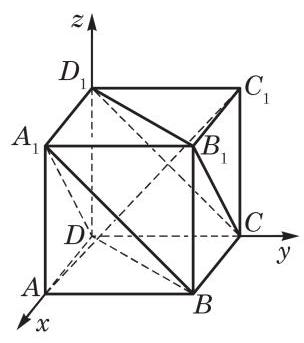
\includegraphics[max width=0.2\textwidth]{images/bo_d7fqvdc91nqc7381i9u0_121_1152_1637_304_343_0.jpg}
\end{center}
\hspace*{3em} 

图 3-4-2

例 2 如图 3-4-2,在正方体 \({ABCD} - {A}_{1}{B}_{1}{C}_{1}{D}_{1}\) 中, 求证:

(1) \(A{C}_{1} \bot\) 平面 \({A}_{1}{BD},A{C}_{1} \bot\) 平面 \(C{D}_{1}{B}_{1}\) ；

(2)平面 \({A}_{1}{BD}//\) 平面 \(C{D}_{1}{B}_{1}\) .

证明(1)设正方体的棱长为 \(a\) . 以点 \(D\) 为原点，分别以 \(\overrightarrow{DA}\text{ 、 }\overrightarrow{DC}\) 与 \(\overrightarrow{D{D}_{1}}\) 的方向为 \(x\text{ 、 }y\) 与 \(z\) 轴的正方向，建立空间直角坐标系, 则得到正方体各顶点的坐标如下:

\[
A\left( {a,0,0}\right) \text{ 、 }B\left( {a,a,0}\right) \text{ 、 }C\left( {0,a,0}\right) \text{ 、 }D\left( {0,0,0}\right) \text{ 、 }
\]

\[
{A}_{1}\left( {a,0,a}\right) \text{ 、 }{B}_{1}\left( {a,a,a}\right) \text{ 、 }{C}_{1}\left( {0,a,a}\right) \text{ 、 }{D}_{1}\left( {0,0,a}\right) .
\]

据此求出直线 \(A{C}_{1}\text{ 、 }{A}_{1}B\text{ 、 }{D}_{1}C\text{ 、 }{A}_{1}D\) 与 \({B}_{1}C\) 的方向向量分别为

\[
\overrightarrow{A{C}_{1}} = \left( {-a,a,a}\right) ,
\]

\[
\overrightarrow{{A}_{1}B} = \overrightarrow{{D}_{1}C} = \left( {0,a, - a}\right) ,
\]

\[
\overrightarrow{{A}_{1}D} = \overrightarrow{{B}_{1}C} = \left( {-a,0, - a}\right) .
\]

计算得到

\[
\overrightarrow{A{C}_{1}} \cdot  \overrightarrow{{A}_{1}B} = \overrightarrow{A{C}_{1}} \cdot  \overrightarrow{{D}_{1}C} = \overrightarrow{A{C}_{1}} \cdot  \overrightarrow{{A}_{1}D} = \overrightarrow{A{C}_{1}} \cdot  \overrightarrow{{B}_{1}C} = 0,
\]

所以

\[
A{C}_{1} \bot  \text{ 平面 }{A}_{1}{BD},A{C}_{1} \bot  \text{ 平面 }C{D}_{1}{B}_{1}\text{ . }
\]

(2)平面 \({A}_{1}{BD}\) 与平面 \(C{D}_{1}{B}_{1}\) 有共同的法向量 \(\overrightarrow{A{C}_{1}}\) ，所以这两个平面平行.

\section*{练习 3.4(1)}

1. 试证明:

(1)两个平面垂直的充要条件是它们的法向量垂直；

(2)两个平面平行的充要条件是它们的法向量平行.

2. 如图，在平面 \(\alpha\) 与平面 \(\beta\) 上分别有不共线的三点 \(A\) 、 \(B\) 、 \(C\) 与 \({A}_{1}\) 、 \({B}_{1}\) 、 \({C}_{1}\) ，假设 \(A{A}_{1}\text{ 、 }B{B}_{1}\) 与 \(C{C}_{1}\) 交于一点 \(O\) ,且 \(\left| {AO}\right|  = \left| {O{A}_{1}}\right| ,\left| {BO}\right|  = \left| {O{B}_{1}}\right| ,\left| {CO}\right|  = \left| {O{C}_{1}}\right|\) . 求证: 平面 \(\alpha //\) 平面 \(\beta\) .

\begin{center}
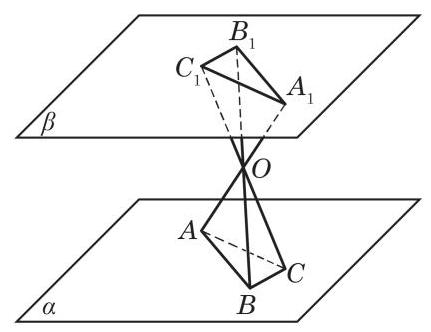
\includegraphics[max width=0.3\textwidth]{images/bo_d7fqvdc91nqc7381i9u0_122_425_1290_431_332_0.jpg}
\end{center}
\hspace*{3em} 

(第 2 题)

\begin{center}
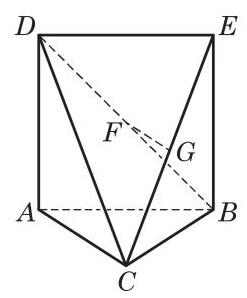
\includegraphics[max width=0.2\textwidth]{images/bo_d7fqvdc91nqc7381i9u0_122_998_1326_247_298_0.jpg}
\end{center}
\hspace*{3em} 

(第 3 题)

3. 如图， \(\bigtriangleup  {ABC}\) 中， \({AC} = {BC} = \frac{\sqrt{2}}{2}{AB}\) ，平面 \({ABED}\bot\) 平面 \({ABC}\) ， \({ABED}\) 是边长为 1 的正方形, \(G\text{ 、 }F\) 分别是 \({EC}\text{ 、 }{BD}\) 的中点. 求证:

(1) \({FG}//\) 平面 \({ABC}\) ；

(2) \({AC} \bot\) 平面 \({EBC}\) .

我们先证明点到平面距离的一般公式.

\begin{center}
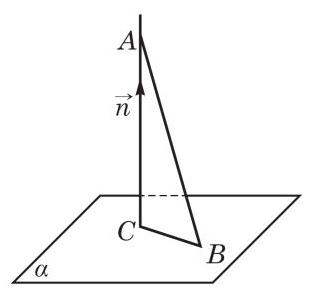
\includegraphics[max width=0.2\textwidth]{images/bo_d7fqvdc91nqc7381i9u0_123_1137_513_310_295_0.jpg}
\end{center}
\hspace*{3em} 

图 3-4-3

如果 \(A\text{ 、 }B\) 是空间中的两个点,其中点 \(B\) 在平面 \(\alpha\) 上, \(\overrightarrow{n}\) 是平面 \(\alpha\) 的一个法向量 (图 3-4-3),那么点 \(A\) 到平面 \(\alpha\) 的距离 \(d\) 是 \(\overrightarrow{AB}\) 在 \(\overrightarrow{n}\) 的方向上的投影 \(\overrightarrow{AC} = \left| \overrightarrow{AB}\right| \cos \langle \overrightarrow{n},\overrightarrow{AB}\rangle \overrightarrow{{n}_{0}}\) 的模,其中 \(\overrightarrow{{n}_{0}}\) 是 \(\overrightarrow{n}\) 的单位向量(称为平面 \(\alpha\) 的单位法向量)，于是

\[
d = \left| \right| \overrightarrow{{n}_{0}}\left| \right| \overrightarrow{AB}\left| {\cos \langle \overrightarrow{n},\overrightarrow{AB}\rangle }\right| .
\]

用向量的数量积表示, 即

\[
d = \left| {\overrightarrow{{n}_{0}} \cdot  \overrightarrow{AB}}\right|  = \frac{\left| \overrightarrow{n} \cdot  \overrightarrow{AB}\right| }{\left| \overrightarrow{n}\right| }.
\]

\begin{center}
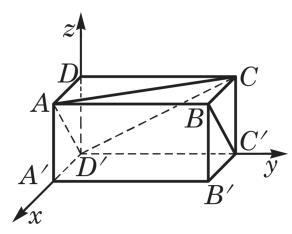
\includegraphics[max width=0.2\textwidth]{images/bo_d7fqvdc91nqc7381i9u0_123_1144_1080_292_234_0.jpg}
\end{center}
\hspace*{3em} 

图 3-4-4

例 3 如图 3-4-4,在长方体 \({ABCD} - {A}^{\prime }{B}^{\prime }{C}^{\prime }{D}^{\prime }\) 中, \(\left| {AB}\right|  = 2,\left| {AD}\right|  = \left| {A{A}^{\prime }}\right|  = 1.\)

(1)求顶点 \({B}^{\prime }\) 到平面 \({D}^{\prime }{AC}\) 的距离；

(2)求直线 \(B{C}^{\prime }\) 到平面 \({D}^{\prime }{AC}\) 的距离.

解(1)如图 3-4-4, 建立空间直角坐标系, 则可得有关点的坐标分别为 \({D}^{\prime }\left( {0,0,0}\right) \text{ 、 }A\left( {1,0,1}\right) \text{ 、 }C\left( {0,2,1}\right)\) 、 \({B}^{\prime }\left( {1,2,0}\right)\) . 所以 \(\overrightarrow{{D}^{\prime }A} = \left( {1,0,1}\right) ,\overrightarrow{{D}^{\prime }C} = \left( {0,2,1}\right)\) .

设平面 \({D}^{\prime }{AC}\) 的法向量为 \(\overrightarrow{n} = \left( {u,v,w}\right)\) ,则 \(\overrightarrow{n} \cdot  \overrightarrow{{D}^{\prime }A} = 0\) , \(\overrightarrow{n} \cdot  \overrightarrow{{D}^{\prime }C} = 0\) . 把各向量的坐标代入,计算得到 \(u + w = 0\) , \({2v} + w = 0\) . 可以取 \(v = 1\) ,从而得到平面 \({D}^{\prime }{AC}\) 的一个法向量为 \(\overrightarrow{n} = \left( {2,1, - 2}\right)\) .

\HRule

平面的法向量不是唯一的, 所以可以给它的某个坐标一个值, 再确定其他坐标的值.

\HRule

因为 \(\overrightarrow{{B}^{\prime }C} = \left( {-1,0,1}\right)\) ,根据上面得到的点到平面的距离公式知,点 \({B}^{\prime }\) 到平面 \({D}^{\prime }{AC}\) 的距离为

\[
d = \frac{\left| \overrightarrow{n} \cdot  \overrightarrow{{B}^{\prime }C}\right| }{\left| \overrightarrow{n}\right| } = \frac{\left| 2 \times  \left( -1\right)  + \left( -2\right)  \times  1\right| }{\sqrt{{2}^{2} + {1}^{2} + {\left( -2\right) }^{2}}} = \frac{4}{3}.
\]

(2)因为 \(\overrightarrow{B{C}^{\prime }} = \overrightarrow{A{D}^{\prime }}\) ，所以 \(B{C}^{\prime }//A{D}^{\prime }\) ，从而 \(B{C}^{\prime }//\) 平面 \({D}^{\prime }{AC}\) ,问题转化为求点 \({C}^{\prime }\left( {0,2,0}\right)\) 到平面 \({D}^{\prime }{AC}\) 的距离. 因为 \(\overrightarrow{{C}^{\prime }C} = \left( {0,0,1}\right)\) ，所以直线 \(B{C}^{\prime }\) 到平面 \({D}^{\prime }{AC}\) 的距离为

\[
\frac{\left| \overrightarrow{n} \cdot  \overrightarrow{{C}^{\prime }C}\right| }{\left| \overrightarrow{n}\right| } = \frac{2}{3}.
\]

求平面的平行线与平面的距离, 只要求平行线上一点到平面的距离; 求两个平行平面的距离, 也只要求其中一个平面上的一个点到另一个平面的距离. ?

\HRule

如何求两条异面直线之间的距离?

\HRule

下一道例题继续用例 2 的题设. 回忆一下, 例 2 已经证明了题中的平面 \({A}_{1}{BD}\) 与平面 \(C{D}_{1}{B}_{1}\) 是平行的.

例 4 设正方体 \({ABCD} - {A}_{1}{B}_{1}{C}_{1}{D}_{1}\) 的棱长为 \(a\) ,求平行平面 \({A}_{1}{BD}\) 与 \(C{D}_{1}{B}_{1}\) 之间的距离.

\begin{center}
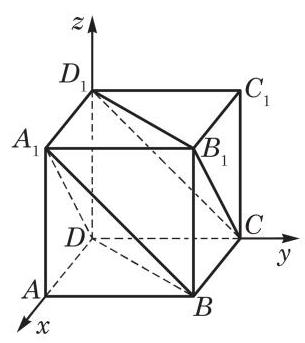
\includegraphics[max width=0.2\textwidth]{images/bo_d7fqvdc91nqc7381i9u0_124_198_843_305_343_0.jpg}
\end{center}
\hspace*{3em} 

图 3-4-5

解 求平行平面 \({A}_{1}{BD}\) 与 \(C{D}_{1}{B}_{1}\) 之间的距离,只要求平面 \(C{D}_{1}{B}_{1}\) 上一点 (例如 \({D}_{1}\) ) 到平面 \({A}_{1}{BD}\) 的距离. 如图 3-4-5,建立空间直角坐标系, 可得点的坐标

\[
D\left( {0,0,0}\right) \text{ 、 }{D}_{1}\left( {0,0,a}\right) \text{ 、 }{A}_{1}\left( {a,0,a}\right) \text{ 、 }B\left( {a,a,0}\right) \text{ , }
\]

于是

\[
\overrightarrow{{D}_{1}D} = \left( {0,0, - a}\right) ,\overrightarrow{D{A}_{1}} = \left( {a,0,a}\right) ,\overrightarrow{DB} = \left( {a,a,0}\right) .
\]

设 \(\overrightarrow{n} = \left( {x,y,z}\right)\) 是平面 \({A}_{1}{BD}\) 的一个法向量,则

\[
\left\{  \begin{array}{l} \overrightarrow{n} \cdot  \overrightarrow{D{A}_{1}} = {ax} + {az} = 0, \\  \overrightarrow{n} \cdot  \overrightarrow{DB} = {ax} + {ay} = 0. \end{array}\right.
\]

因为 \(a \neq  0\) ,所以

\[
\left\{  \begin{array}{l} x + z = 0, \\  x + y = 0. \end{array}\right.
\]

不妨取 \(z = 1\) ,则 \(x =  - 1,y = 1\) ,就得到平面 \({A}_{1}{BD}\) 的一个法向量 \(\overrightarrow{n} = \left( {-1,1,1}\right)\) . 这样,点 \({D}_{1}\) 到平面 \({A}_{1}{BD}\) 的距离为

\[
d = \frac{\left| \overrightarrow{n} \cdot  \overrightarrow{{D}_{1}D}\right| }{\left| \overrightarrow{n}\right| } = \frac{\left| \left( -1\right)  \times  0 + 1 \times  0 + 1 \times  \left( -a\right) \right| }{\sqrt{{\left( -1\right) }^{2} + {1}^{2} + {1}^{2}}} = \frac{\sqrt{3}}{3}a.
\]

因此,平行平面 \({A}_{1}{BD}\) 与平面 \(C{D}_{1}{B}_{1}\) 之间的距离为 \(\frac{\sqrt{3}}{3}a\) .

\section*{练习 \({3.4}\left( 2\right)\)}

1. 已知三棱锥 \(A - {BCD}\) 的三条侧棱 \({AB}\) 、 \({AC}\) 、 \({AD}\) 两两垂直，且 \(\left| {AB}\right|  = 1\) ， \(\left| {AC}\right|  =\) 2, \(\left| {AD}\right|  = 3\) . 求顶点 \(A\) 到平面 \({BCD}\) 的距离.

2. 在练习 3.4(1)第 3 题的题设条件下，求直线 \({FG}\) 与平面 \({ABC}\) 的距离.

\section*{3 求角的大小}

\begin{center}
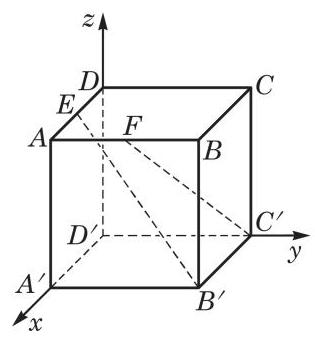
\includegraphics[max width=0.2\textwidth]{images/bo_d7fqvdc91nqc7381i9u0_125_1141_461_315_338_0.jpg}
\end{center}
\hspace*{3em} 

图 3-4-6

例 5 如图 3-4-6,在正方体 \({ABCD} - {A}^{\prime }{B}^{\prime }{C}^{\prime }{D}^{\prime }\) 中, \(E\) 、 \(F\) 分别是 \({AD}\text{ 、 }{AB}\) 的中点. 求直线 \({B}^{\prime }E\) 与 \({C}^{\prime }F\) 所成角的大小.

解 设正方体的棱长为 \(a\) . 以点 \({D}^{\prime }\) 为原点,分别以 \(\overrightarrow{{D}^{\prime }{A}^{\prime }}\) 、 \(\overrightarrow{{D}^{\prime }{C}^{\prime }}\) 与 \(\overrightarrow{{D}^{\prime }D}\) 的方向为 \(x\text{ 、 }y\) 与 \(z\) 轴的正方向,建立空间直角坐标系,则可得有关点的坐标分别为 \({B}^{\prime }\left( {a,a,0}\right) \text{ 、 }E\left( {\frac{a}{2},0,a}\right)\) 、 \({C}^{\prime }\left( {0,a,0}\right) \text{ 、 }F\left( {a,\frac{a}{2},a}\right)\) ,因此,直线 \({B}^{\prime }E\) 与 \({C}^{\prime }F\) 的方向向量分别是

\[
\overrightarrow{{B}^{\prime }E} = \left( {-\frac{a}{2}, - a,a}\right) \text{ 与 }\overrightarrow{{C}^{\prime }F} = \left( {a, - \frac{a}{2},a}\right) .
\]

从而

\[
\cos \left\langle  {\overrightarrow{{B}^{\prime }E},\overrightarrow{{C}^{\prime }F}}\right\rangle   = \frac{\overrightarrow{{B}^{\prime }E} \cdot  \overrightarrow{{C}^{\prime }F}}{\left| \overrightarrow{{B}^{\prime }E}\right| \left| \overrightarrow{{C}^{\prime }F}\right| } = \frac{4}{9}.
\]

所以,直线 \({B}^{\prime }E\) 与 \({C}^{\prime }F\) 所成角的大小为 \(\arccos \frac{4}{9}\) .

例 5 中的两条直线是异面直线. 事实上, 用向量方法求两条直线所成的角时, 无须区分它们是否为异面直线. 但要注意,如果两条直线 \({l}_{1}\) 与 \({l}_{2}\) 的方向向量分别是 \(\overrightarrow{{r}_{1}}\) 与 \(\overrightarrow{{r}_{2}}\) ,当求出的方向向量的夹角 \(\left\langle  {\overrightarrow{{r}_{1}},\overrightarrow{{r}_{2}}}\right\rangle   > \frac{\pi }{2}\) 时, \({l}_{1}\) 与 \({l}_{2}\) 所成的角 \(\theta\) 是它的补角 \(\pi  - \left\langle  {\overrightarrow{{r}_{1}},\overrightarrow{{r}_{2}}}\right\rangle\) . 因为我们约定两条直线所成角的取值在 0 和 \(\frac{\pi }{2}\) 之间. 所以,用方向向量 \({\overrightarrow{r}}_{1}\) 与 \({\overrightarrow{r}}_{2}\) 表达的两条直线所成角 \(\theta\) 的大小的公式为

\[
\cos \theta  = \frac{\left| \overrightarrow{{r}_{1}} \cdot  \overrightarrow{{r}_{2}}\right| }{\left| \overrightarrow{{r}_{1}}\right| \left| \overrightarrow{{r}_{2}}\right| }.
\]

立体几何中常见的有关角的问题还有直线与平面所成的角和平面与平面所成的角(二面角). 确定这两类角的大小, 都可以通过转化为直线的方向向量和平面的法向量两个向量夹角的问题加以解决. 当然, 为得到最终的解答, 必须知道所要讨论的角与转化后的向量夹角的关系.

先考虑直线与平面所成的角. 从图 3-4-7 可以看出, 直线与平面垂线(法向量所在直线)所成的角和直线与平面所成的角的关系:如果直线与平面所成的角为 \(\theta\) ，那么直线与平面垂线(法向量所在直线) 所成的角为 \(\frac{\pi }{2} - \theta\) . 因此,如果直线的一个方向向量为 \(\overrightarrow{r}\) ,平面的一个法向量为 \(\overrightarrow{n}\) ,那么直线与平面所成的角 \(\theta\) 的大小由如下公式确定:

\[
\sin \theta  = \cos \left( {\frac{\pi }{2} - \theta }\right)  = \frac{\left| \overrightarrow{r} \cdot  \overrightarrow{n}\right| }{\left| \overrightarrow{r}\right| \left| \overrightarrow{n}\right| }.
\]

\begin{center}
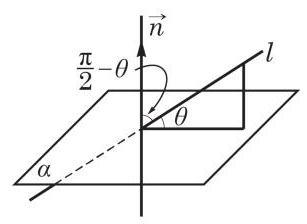
\includegraphics[max width=0.2\textwidth]{images/bo_d7fqvdc91nqc7381i9u0_126_180_352_307_224_0.jpg}
\end{center}
\hspace*{3em} 

图 3-4-7

\begin{center}
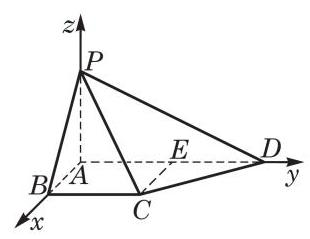
\includegraphics[max width=0.2\textwidth]{images/bo_d7fqvdc91nqc7381i9u0_126_179_910_310_239_0.jpg}
\end{center}
\hspace*{3em} 

图 3-4-8

例 6 如图 3-4-8,在四棱锥 \(P - {ABCD}\) 中, \({PA} \bot\) 平面 \({ABCD},{AB} \bot  {AD},{BC}//{AD},\left| {PA}\right|  = \left| {AB}\right|  = \left| {BC}\right|  = 1\) , \(\left| {CD}\right|  = \sqrt{2},\angle {CDA} = {45}^{ \circ  }\) . 求直线 \({PB}\) 与平面 \({PCD}\) 所成角的大小.

解 因为 \({PA} \bot\) 平面 \({ABCD},{AB} \bot  {AD}\) ,则可取点 \(A\) 为原点,分别以 \(\overrightarrow{AB}\text{ 、 }\overrightarrow{AD}\) 与 \(\overrightarrow{AP}\) 的方向为 \(x\text{ 、 }y\) 与 \(z\) 轴的正方向,建立空间直角坐标系. 作 \({CE}//{BA}\) 交 \({AD}\) 于点 \(E\) ，则 \(\left| {CE}\right|  = 1\) . 又 \(\left| {CD}\right|  = \sqrt{2}\) ,由勾股定理,易知 \(\bigtriangleup {CDE}\) 是等腰直角三角形,从而 \(\left| {ED}\right|  = 1,\left| {AD}\right|  = 2\) . 于是,可得有关点的坐标分别为 \(A\left( {0,0,0}\right)\) 、 \(B\left( {1,0,0}\right) \text{ 、 }C\left( {1,1,0}\right) \text{ 、 }D\left( {0,2,0}\right) \text{ 、 }P\left( {0,0,1}\right)\) ,所以 \(\overrightarrow{PB} = \left( {1,0, - 1}\right) ,\overrightarrow{CD} = \left( {-1,1,0}\right) ,\overrightarrow{PD} = \left( {0,2, - 1}\right) .\)

设平面 \({PCD}\) 的法向量为 \(\overrightarrow{n} = \left( {u,v,w}\right)\) ,则 \(\overrightarrow{n} \cdot  \overrightarrow{CD} = 0\) , \(\overrightarrow{n} \cdot  \overrightarrow{PD} = 0\) . 即 \(- u + v = 0,{2v} - w = 0\) . 取 \(v = 1\) ,从而得到平面 \({PCD}\) 的一个法向量为 \(\overrightarrow{n} = \left( {1,1,2}\right)\) .

设直线 \({PB}\) 与平面 \({PCD}\) 所成角的大小为 \(\theta \left( {0 \leq  \theta  \leq  \frac{\pi }{2}}\right)\) ,则

\[
\sin \theta  = \cos \left( {\frac{\pi }{2} - \theta }\right)  = \frac{\left| \overrightarrow{n} \cdot  \overrightarrow{PB}\right| }{\left| \overrightarrow{n}\right| \left| \overrightarrow{PB}\right| } = \frac{\sqrt{3}}{6}.
\]

所以,直线 \({PB}\) 与平面 \({PCD}\) 所成角的大小为 \(\arcsin \frac{\sqrt{3}}{6}\) .

\section*{练习 3.4(3)}

1. 如图,四边形 \({ABCD}\) 是矩形, \({PA} \bot\) 平面 \({ABCD},E\) 是线段 \({PA}\) 的中点. 已知 \(\left| {PA}\right|  = 2,\left| {AB}\right|  = \sqrt{3},\left| {BC}\right|  = 1\) . 求异面直线 \({BE}\) 与 \({PC}\) 所成角的大小.

\begin{center}
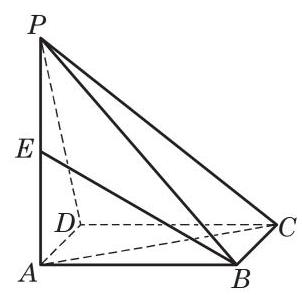
\includegraphics[max width=0.2\textwidth]{images/bo_d7fqvdc91nqc7381i9u0_127_383_492_303_295_0.jpg}
\end{center}
\hspace*{3em} 

(第 1 题)

\begin{center}
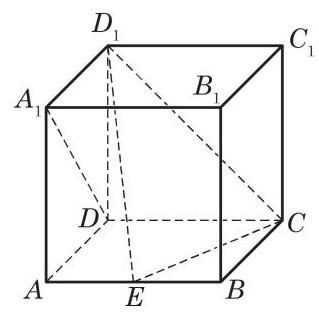
\includegraphics[max width=0.2\textwidth]{images/bo_d7fqvdc91nqc7381i9u0_127_909_475_319_314_0.jpg}
\end{center}
\hspace*{3em} 

(第 2 题)

2. 如图,在棱长为 1 的正方体 \({ABCD} - {A}_{1}{B}_{1}{C}_{1}{D}_{1}\) 中, \(E\) 是棱 \({AB}\) 上的动点.

(1)求证: \(D{A}_{1}\bot E{D}_{1}\) ；

(2)确定点 \(E\) 的位置，使得直线 \(D{A}_{1}\) 与平面 \({CE}{D}_{1}\) 所成的角是 \({45}^{ \circ  }\) .

现在考虑二面角的平面角和它的两个半平面所在平面的法向量夹角大小的关系. 如图 3-4-9, 一个平面的法向量垂直于该平面上的所有直线，所以法向量夹角的两条边垂直于二面角的平面角相应的边. 从平面几何知道, 这样两个角或者相等, 或者互补.

\begin{center}
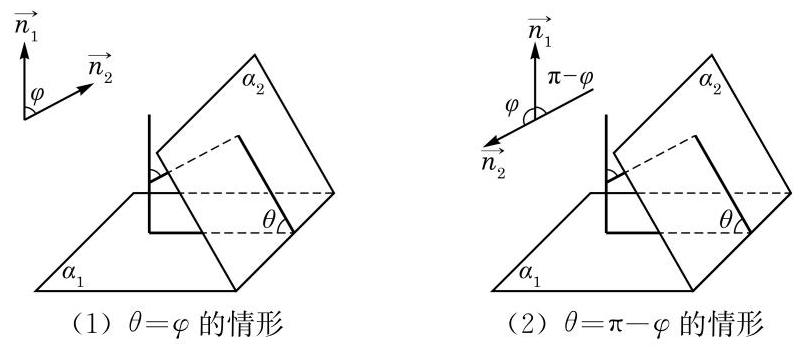
\includegraphics[max width=0.6\textwidth]{images/bo_d7fqvdc91nqc7381i9u0_127_222_1351_804_349_0.jpg}
\end{center}
\hspace*{3em} 

图 3-4-9

因此,如果 \(\overrightarrow{{n}_{1}}\) 与 \(\overrightarrow{{n}_{2}}\) 分别是两个平面的法向量,那么这两个平面所成的锐二面角(或直二面角) \(\theta\) 的大小由如下公式确定:

\[
\cos \theta  = \frac{\left| \overrightarrow{{n}_{1}} \cdot  \overrightarrow{{n}_{2}}\right| }{\left| \overrightarrow{{n}_{1}}\right| \left| \overrightarrow{{n}_{2}}\right| }.
\]

例 7 如图 3-4-10(1),在正四棱锥 \(P - {ABCD}\) 中, \(\left| {PA}\right|  = \; \left| {AB}\right|  = 2\sqrt{2},E\text{ 、 }F\) 分别为 \({PB}\text{ 、 }{PD}\) 的中点. 若平面 \({AEF}\) 与棱 \({PC}\) 交于点 \(G\) ,求平面 \({AEGF}\) 与平面 \({ABCD}\) 所成二面角的大小.

\begin{center}
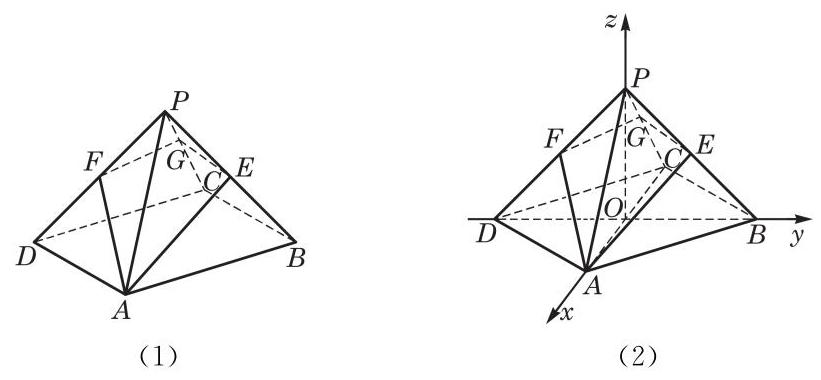
\includegraphics[max width=0.7\textwidth]{images/bo_d7fqvdc91nqc7381i9u0_128_611_437_821_380_0.jpg}
\end{center}
\hspace*{3em} 

图 3-4-10

解 如图 3-4-10(2),连接 \({AC}\text{ 、 }{BD}\) 交于点 \(O\) ,则 \({OA}\) 、 \({OB}\text{ 、 }{OP}\) 两两互相垂直. 以点 \(O\) 为坐标原点,分别以 \(\overrightarrow{OA}\) 、 \(\overrightarrow{OB}\text{ 、 }\overrightarrow{OP}\) 的方向为 \(x\text{ 、 }y\) 与 \(z\) 轴的正方向,建立空间直角坐标系.

因为 \(\left| {PA}\right|  = \left| {AB}\right|  = 2\sqrt{2}\) ,由勾股定理,易知 \(\left| {OA}\right|  = \left| {OB}\right|  = \; \left| {OP}\right|  = 2\) ,从而可得有关点的坐标分别为 \(A\left( {2,0,0}\right) \text{ 、 }B\left( {0,2,0}\right)\) 、 \(C\left( {-2,0,0}\right) \text{ 、 }D\left( {0, - 2,0}\right) \text{ 、 }P\left( {0,0,2}\right) \text{ 、 }E\left( {0,1,1}\right) \text{ 、 }F\left( {0, - 1,1}\right) .\) 所以 \(\overrightarrow{AE} = \left( {-2,1,1}\right) ,\overrightarrow{AF} = \left( {-2, - 1,1}\right)\) .

设平面 \({AEGF}\) 的法向量为 \(\overrightarrow{n} = \left( {u,v,w}\right)\) ,由 \(\overrightarrow{n} \cdot  \overrightarrow{AE} = 0\) 与 \(\overrightarrow{n} \cdot  \overrightarrow{AF} = 0\) ,推出关系式 \(- {2u} + v + w = 0\) 与 \(- {2u} - v + w = 0\) . 可取 \(u = 1\) ,解得 \(v = 0,w = 2\) ,从而得到平面 \({AEGF}\) 的一个法向量 \(\overrightarrow{n} = \left( {1,0,2}\right)\) .

平面 \({ABCD}\) 的法向量显然可取为 \(\overrightarrow{m} = \left( {0,0,1}\right)\) ,从而

\[
\cos \langle \overrightarrow{m},\overrightarrow{n}\rangle  = \frac{\overrightarrow{m} \cdot  \overrightarrow{n}}{\left| \overrightarrow{m}\right| \left| \overrightarrow{n}\right| } = \frac{2}{1 \times  \sqrt{5}} = \frac{2\sqrt{5}}{5}.
\]

所以,平面 \({AEGF}\) 与平面 \({ABCD}\) 所成的二面角是 \(\arccos \frac{2\sqrt{5}}{5}\) 与 \(\pi  - \arccos \frac{2\sqrt{5}}{5}\) (前者是锐二面角).

\section*{练习 3.4(4)}

1. 在正方体 \({ABCD} - {A}^{\prime }{B}^{\prime }{C}^{\prime }{D}^{\prime }\) 中, \(E\text{ 、 }F\) 分别是 \({BC}\text{ 、 }{CD}\) 的中点. 求二面角 \(B - {B}^{\prime }E - F\) 的大小.

2. 如图,在正方体 \({ABCD} - {A}_{1}{B}_{1}{C}_{1}{D}_{1}\) 中,求平面 \(D{A}_{1}B\) 与平面 \({A}_{1}{B}_{1}{C}_{1}{D}_{1}\) 所成二面角的正弦值.

\begin{center}
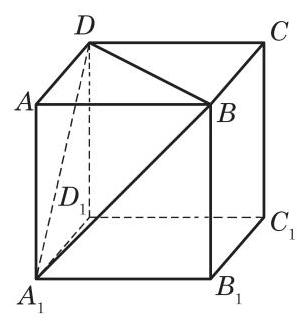
\includegraphics[max width=0.2\textwidth]{images/bo_d7fqvdc91nqc7381i9u0_129_439_607_303_321_0.jpg}
\end{center}
\hspace*{3em} 

(第 2 题)

\begin{center}
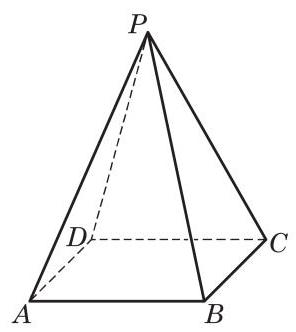
\includegraphics[max width=0.2\textwidth]{images/bo_d7fqvdc91nqc7381i9u0_129_882_592_296_332_0.jpg}
\end{center}
\hspace*{3em} 

(第 4 题)

3. 如图，在正四棱锥 \(P - {ABCD}\) 中，底面边长为 2，高为 3. 求二面角 \(A - {PB} - C\) 的大小.

\section*{习题 3.4}

\section*{A 组}

1. 在正四棱柱 \({ABCD} - {A}_{1}{B}_{1}{C}_{1}{D}_{1}\) 中, \(\left| {A{A}_{1}}\right|  = 2\left| {AB}\right|  = 2\) , \(E\) 为 \(A{A}_{1}\) 的中点. 求异面直线 \({BE}\) 与 \(C{D}_{1}\) 所成角的大小.

2. 在正方体 \({ABCD} - {A}_{1}{B}_{1}{C}_{1}{D}_{1}\) 中, \(M\text{ 、 }N\text{ 、 }P\) 分别是 \(C{C}_{1}\text{ 、 }{B}_{1}{C}_{1}\text{ 、 }{C}_{1}{D}_{1}\) 的中点. 求证: 平面 \({MNP}//\) 平面 \({A}_{1}{BD}\) .

3. 在正方体 \({ABCD} - {A}_{1}{B}_{1}{C}_{1}{D}_{1}\) 中,求 \(B{B}_{1}\) 与平面 \({AC}{D}_{1}\) 所成角的大小.

\begin{center}
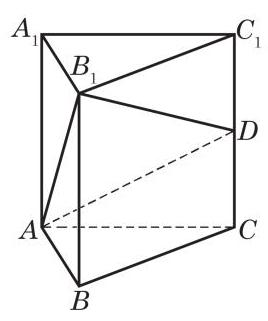
\includegraphics[max width=0.2\textwidth]{images/bo_d7fqvdc91nqc7381i9u0_129_1196_1762_268_321_0.jpg}
\end{center}
\hspace*{3em} 

(第 4 题)

4. 如图,已知正三棱柱 \({ABC} - {A}_{1}{B}_{1}{C}_{1}\) 的各条棱长均为 \(a,D\) 是棱 \(C{C}_{1}\) 的中点. 求证: 平面 \(A{B}_{1}D \bot\) 平面 \({AB}{B}_{1}{A}_{1}\) .

5. 如图,已知 \(P\) 为平面 \({ABC}\) 外一点, \({AP}\text{ 、 }{AB}\text{ 、 }{AC}\) 两两互相垂直,过 \({AC}\) 的中点 \(D\) 作 \({ED} \bot\) 平面 \({ABC}\) ,且 \(\left| {ED}\right|  = 1,\left| {PA}\right|  = 2\) , \(\left| {AC}\right|  = 2\) ,多面体 \(B - {PADE}\) 的体积是 \(\frac{\sqrt{3}}{3}\) . 求平面 \({PBE}\) 与平面 \({ABC}\) 所成二面角的大小.

\begin{center}
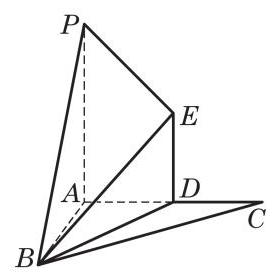
\includegraphics[max width=0.2\textwidth]{images/bo_d7fqvdc91nqc7381i9u0_130_406_288_273_277_0.jpg}
\end{center}
\hspace*{3em} 

(第 5 题)

\begin{center}
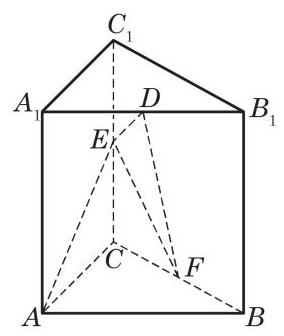
\includegraphics[max width=0.2\textwidth]{images/bo_d7fqvdc91nqc7381i9u0_130_982_229_284_336_0.jpg}
\end{center}
\hspace*{3em} 

(第 6 题)

6. 如图,在直棱柱 \({ABC} - {A}_{1}{B}_{1}{C}_{1}\) 中, \(\left| {A{A}_{1}}\right|  = \left| {AB}\right|  = \left| {AC}\right|  = 2,{AB} \bot  {AC},D\text{ 、 }E\text{ 、 }F\) 分别是 \({A}_{1}{B}_{1}\text{ 、 }C{C}_{1}\text{ 、 }{BC}\) 的中点.

(1)求 \({AE}\) 与平面 \({DEF}\) 所成角的大小；

(2)求 \(A\) 到平面 \({DEF}\) 的距离.

\section*{B 组}

1. 如图,在空间四边形 \({ABCD}\) 中, \(\left| {AC}\right|  = \left| {AD}\right| ,\angle {BAC} = \angle {BAD}\) . 求证: \({CD} \bot  {AB}\) .

\begin{center}
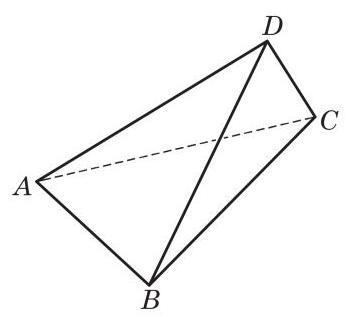
\includegraphics[max width=0.2\textwidth]{images/bo_d7fqvdc91nqc7381i9u0_130_399_1125_348_317_0.jpg}
\end{center}
\hspace*{3em} 

(第 1 题)

\begin{center}
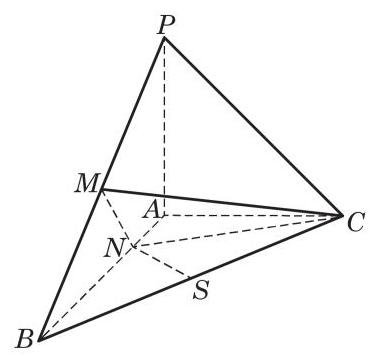
\includegraphics[max width=0.3\textwidth]{images/bo_d7fqvdc91nqc7381i9u0_130_918_1086_373_357_0.jpg}
\end{center}
\hspace*{3em} 

(第 2 题)

2. 如图,在三棱锥 \(P - {ABC}\) 中, \({PA} \bot\) 平面 \({ABC},{AB} \bot  {AC},\left| {PA}\right|  = \left| {AC}\right|  = \frac{1}{2}\left| {AB}\right|\) , \(M\text{ 、 }S\) 分别为 \({PB}\text{ 、 }{BC}\) 的中点, \(N\) 为 \({AB}\) 上一点, \(\left| {BN}\right|  = 3\left| {NA}\right|\) .

(1)求证: \({CM}\bot {SN}\) ；

\begin{center}
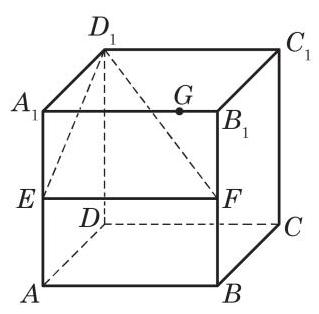
\includegraphics[max width=0.2\textwidth]{images/bo_d7fqvdc91nqc7381i9u0_130_1175_1743_319_314_0.jpg}
\end{center}
\hspace*{3em} 

(第 5 题)

(2)求二面角 \(P - {BC} - A\) 的大小.

3. 在正方体 \({ABCD} - {A}_{1}{B}_{1}{C}_{1}{D}_{1}\) 中,设 \({AB}\text{ 、 }D{D}_{1}\) 的中点分别为 \(M\text{ 、 }N\) . 求直线 \({B}_{1}M\) 与 \({CN}\) 所成角的大小.

4. 过边长为 1 的正方形 \({ABCD}\) 的顶点 \(A\) ,作长度为 1 的线段 \({AE} \bot\) 平面 \({ABCD}\) . 求平面 \({ADE}\) 与平面 \({BCE}\) 所成二面角的大小.

5. 如图,在棱长为 1 的正方体 \({ABCD} - {A}_{1}{B}_{1}{C}_{1}{D}_{1}\) 中, \(E\text{ 、 }F\) 分别为棱 \(A{A}_{1}\text{ 、 }B{B}_{1}\) 的中点, \(G\) 为棱 \({A}_{1}{B}_{1}\) 上的一点. 求点 \(G\) 到平面 \({D}_{1}{EF}\) 的距离.

\section*{内容提要}

\section*{1. 空间向量的概念与运算}

(1)空间向量的定义和相关概念(模、零向量、单位向量、平行向量、相等向量、负向量等)与平面向量情形相同.

(2)对只与一组共面向量相关的问题，有关平面向量的定义与结论均适用. 特别地， 平面向量运算(加法、减法、与实数的乘法、数量积)的定义与性质直接适用于空间向量.

2. 向量共面的充要条件与空间向量基本定理

(1)向量共面的充要条件:如果 \(\overrightarrow{{e}_{1}}\) 与 \(\overrightarrow{{e}_{2}}\) 是两个不平行的向量，那么空间中的向量 \(\overrightarrow{a}\) 与 \(\overrightarrow{{e}_{1}}\text{ 、 }\overrightarrow{{e}_{2}}\) 共面的充要条件是:存在唯一的一对实数 \(\lambda\) 与 \(\mu\) ，使得 \(\overrightarrow{a} = \lambda \overrightarrow{{e}_{1}} + \mu \overrightarrow{{e}_{2}}\) .

(2)空间向量基本定理:如果 \(\overrightarrow{{e}_{1}}\text{ 、 }\overrightarrow{{e}_{2}}\) 与 \(\overrightarrow{{e}_{3}}\) 是不共面的向量，那么对于空间中任一向量 \(\overrightarrow{a}\) ,存在唯一的一组实数 \(\lambda \text{ 、 }\mu\) 与 \(\nu\) ,使得 \(\overrightarrow{a} = \lambda {\overrightarrow{e}}_{1} + \mu {\overrightarrow{e}}_{2} + \nu {\overrightarrow{e}}_{3}\) .

3. 空间向量的坐标表示

(1)空间向量的坐标表示:建立空间直角坐标系，把向量 \(\overrightarrow{p}\) 的起点放在坐标原点，该向量就直接用它的终点坐标 \(\left( {x,y,z}\right)\) 表示为 \(\overrightarrow{p} = \left( {x,y,z}\right)\) ，这个表示的意义是: \(\overrightarrow{p}\) 是坐标轴正方向上的单位向量 \(\overrightarrow{i}\text{ 、 }\overrightarrow{j}\) 与 \(\overrightarrow{k}\) 的线性组合 \(\overrightarrow{p} = x\overrightarrow{i} + y\overrightarrow{j} + z\overrightarrow{k}\) .

(2)给定空间两点 \(A\left( {{x}_{1},{y}_{1},{z}_{1}}\right)\) 与 \(B\left( {{x}_{2},{y}_{2},{z}_{2}}\right)\) ，则 \(\overrightarrow{AB} = \left( {{x}_{2} - {x}_{1},{y}_{2} - {y}_{1},{z}_{2} - {z}_{1}}\right)\) .

4. 坐标表示下的空间向量运算

设向量 \(\overrightarrow{a} = \left( {{x}_{1},{y}_{1},{z}_{1}}\right) ,\overrightarrow{b} = \left( {{x}_{2},{y}_{2},{z}_{2}}\right)\) ,则

(1) \(\left| \overrightarrow{a}\right|  = \sqrt{{x}_{1}^{2} + {y}_{1}^{2} + {z}_{1}^{2}}\) ；

(2) \(\overrightarrow{a} \pm  \overrightarrow{b} = \left( {{x}_{1} \pm  {x}_{2},{y}_{1} \pm  {y}_{2},{z}_{1} \pm  {z}_{2}}\right)\) ；

(3) \(\lambda \overrightarrow{a} = \left( {\lambda {x}_{1},\lambda {y}_{1},\lambda {z}_{1}}\right) ,\lambda  \in  \mathbf{R}\) ；

(4) \(\overrightarrow{a} \cdot  \overrightarrow{b} = {x}_{1}{x}_{2} + {y}_{1}{y}_{2} + {z}_{1}{z}_{2}\) .

5. 空间向量的夹角、平行与垂直

设向量 \(\overrightarrow{a} = \left( {{x}_{1},{y}_{1},{z}_{1}}\right) ,\overrightarrow{b} = \left( {{x}_{2},{y}_{2},{z}_{2}}\right)\) 均为非零向量,则

(1) \(\cos \langle \overrightarrow{a},\overrightarrow{b}\rangle  = \frac{\overrightarrow{a} \cdot  \overrightarrow{b}}{\left| \overrightarrow{a}\right| \left| \overrightarrow{b}\right| } = \frac{{x}_{1}{x}_{2} + {y}_{1}{y}_{2} + {z}_{1}{z}_{2}}{\sqrt{{x}_{1}^{2} + {y}_{1}^{2} + {z}_{1}^{2}}\sqrt{{x}_{2}^{2} + {y}_{2}^{2} + {z}_{2}^{2}}}\) ;

(2) \(\overrightarrow{a}//\overrightarrow{b} \Leftrightarrow  \overrightarrow{a} = \lambda \overrightarrow{b},\lambda  \in  \mathbf{R} \Leftrightarrow  {x}_{1} = \lambda {x}_{2},{y}_{1} = \lambda {y}_{2},{z}_{1} = \lambda {z}_{2},\lambda  \in  \mathbf{R}\) ；

(3) \(\overrightarrow{a} \bot  \overrightarrow{b} \Leftrightarrow  \overrightarrow{a} \cdot  \overrightarrow{b} = 0 \Leftrightarrow  {x}_{1}{x}_{2} + {y}_{1}{y}_{2} + {z}_{1}{z}_{2} = 0\) .

6. 空间向量在立体几何中的应用

空间中的直线和平面可以分别通过方向向量和法向量与空间向量联系起来，从而把立体几何的许多问题化为向量的问题加以解决.

(1)空间直线与平面之间的平行与垂直

 \circled{1}  两条直线平行的充要条件是它们的方向向量平行；两条直线垂直的充要条件是它们的方向向量垂直.

 \circled{2}  直线和平面垂直的充要条件是直线的方向向量为平面的法向量；平面外一条直线和平面平行的充要条件是直线的方向向量垂直于平面的法向量.

 \circled{3}  两个平面垂直的充要条件是其中一个平面过另一个平面的一个法向量；两个平面平行的充要条件是它们的法向量平行.

(2)求距离

 \circled{1}  平面外一点 \(A\) 到平面的距离 \(d\) 由公式

\[
d = \frac{\left| \overrightarrow{n} \cdot  \overrightarrow{AB}\right| }{\left| \overrightarrow{n}\right| }
\]

给出，其中 \(\overrightarrow{n}\) 是平面的一个法向量， \(B\) 是平面上任意一点.

 \circled{2}  平面的平行线到平面的距离、平行平面间的距离均化为点到平面的距离来处理.

(3)求角的大小

 \circled{1}  具有方向向量 \(\overrightarrow{{r}_{1}}\) 与 \(\overrightarrow{{r}_{2}}\) 的两条直线的所成角 \(\theta\) 的大小由如下公式确定:

\[
\cos \theta  = \frac{\left| \overrightarrow{{r}_{1}} \cdot  \overrightarrow{{r}_{2}}\right| }{\left| \overrightarrow{{r}_{1}}\right| \left| \overrightarrow{{r}_{2}}\right| }.
\]

 \circled{2}  具有方向向量 \(\overrightarrow{r}\) 的直线与具有法向量 \(\overrightarrow{n}\) 的平面的所成角 \(\theta\) 的大小由如下公式确定:

\[
\sin \theta  = \frac{\left| \overrightarrow{r} \cdot  \overrightarrow{n}\right| }{\left| \overrightarrow{r}\right| \left| \overrightarrow{n}\right| }
\]

 \circled{3}  具有法向量 \(\overrightarrow{{n}_{1}}\) 与 \(\overrightarrow{{n}_{2}}\) 的两个平面所成的锐二面角(或直二面角) \(\theta\) 的大小由如下公式确定:

\[
\cos \theta  = \frac{\left| \overrightarrow{{n}_{1}} \cdot  \overrightarrow{{n}_{2}}\right| }{\left| \overrightarrow{{n}_{1}}\right| \left| \overrightarrow{{n}_{2}}\right| }.
\]

\section*{复习题}

\section*{A 组}

1. 求连接点 \(A\left( {x,y,z}\right)\) 与点 \(B\left( {{x}^{\prime },{y}^{\prime },{z}^{\prime }}\right)\) 的线段 \({AB}\) 的中点 \(M\) 的坐标.

2. 设正四面体 \({ABCD}\) 的棱长为 \(a,E\) 为 \({BC}\) 的中点, \(F\) 为 \({CD}\) 的中点. 求 \(\overrightarrow{BF} \cdot  \overrightarrow{AE}\) .

3. 给定点 \(A\left( {1,0,0}\right) \text{ 、 }B\left( {3,1,1}\right) \text{ 、 }C\left( {2,0,1}\right)\) 与点 \(D\left( {5, - 4,3}\right)\) .

(1)求 \(\overrightarrow{AD}\) 在 \(\overrightarrow{AB}\) 、 \(\overrightarrow{BC}\) 、 \(\overrightarrow{CA}\) 方向上的投影向量；

(2)求点 \(D\) 到平面 \({ABC}\) 的距离.

\begin{center}
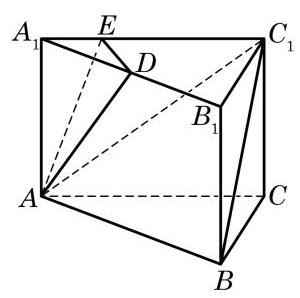
\includegraphics[max width=0.2\textwidth]{images/bo_d7fqvdc91nqc7381i9u0_133_1159_460_300_298_0.jpg}
\end{center}
\hspace*{3em} 

(第 4 题)

4. 如图,在正三棱柱 \({ABC} - {A}_{1}{B}_{1}{C}_{1}\) 中, \(\left| {AB}\right|  = \sqrt{2}\left| {A{A}_{1}}\right|\) , \(D\) 是 \({A}_{1}{B}_{1}\) 的中点,点 \(E\) 在 \({A}_{1}{C}_{1}\) 上,且 \({DE} \bot  {AE}\) .

(1)求证:平面 \({ADE} \bot\) 平面 \({AC}{C}_{1}{A}_{1}\) ；

(2)求直线 \({AD}\) 和平面 \({AB}{C}_{1}\) 所成角的大小.

5. 已知正四棱锥的体积为 12,底面对角线的长为 \(2\sqrt{6}\) . 求侧面与底面所成二面角的大小.

6. 如图,已知 \({ABCD} - {A}_{1}{B}_{1}{C}_{1}{D}_{1}\) 是底面边长为 1 的正四棱柱, \({O}_{1}\) 是 \({A}_{1}{C}_{1}\) 和 \({B}_{1}{D}_{1}\) 的交点.

(1)设 \(A{B}_{1}\) 与底面 \({A}_{1}{B}_{1}{C}_{1}{D}_{1}\) 所成角的大小为 \(\alpha\) ，二面角 \(A - {B}_{1}{D}_{1} - {A}_{1}\) 的大小为 \(\beta\) . 求证: \(\tan \beta  = \sqrt{2}\tan \alpha\) ;

(2)若点 \(C\) 到平面 \(A{B}_{1}{D}_{1}\) 的距离为 \(\frac{4}{3}\) ，求此正四棱柱的高.

\begin{center}
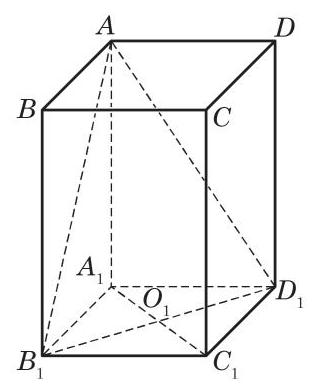
\includegraphics[max width=0.2\textwidth]{images/bo_d7fqvdc91nqc7381i9u0_133_373_1163_312_388_0.jpg}
\end{center}
\hspace*{3em} 

(第 6 题)

\begin{center}
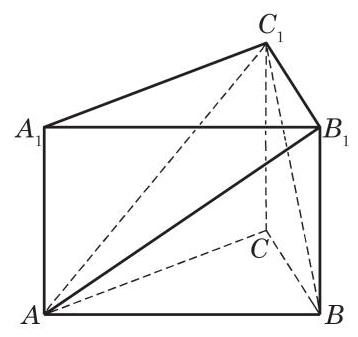
\includegraphics[max width=0.3\textwidth]{images/bo_d7fqvdc91nqc7381i9u0_133_867_1199_358_337_0.jpg}
\end{center}
\hspace*{3em} 

(第 7 题)

7. 如图,在直三棱柱 \({ABC} - {A}_{1}{B}_{1}{C}_{1}\) 中, \(\angle {ACB} = {90}^{ \circ  },\left| {AC}\right|  = \left| {BC}\right|  = \left| {C{C}_{1}}\right|  = 2\) .

(1)求证: \(A{B}_{1} \bot  B{C}_{1}\) ；

(2)求点 \(B\) 到平面 \(A{B}_{1}{C}_{1}\) 的距离.

8. 如图,四棱锥 \(P - {ABCD}\) 的底面 \({ABCD}\) 为梯形, \({AD}//{BC},{AB} \bot  {BC},\left| {AB}\right|  = 1\) , \(\left| {AD}\right|  = 3,\angle {ADC} = {45}^{ \circ  }\) ,且 \({PA} \bot\) 平面 \({ABCD},\left| {PA}\right|  = 1\) .

(1)求异面直线 \({PB}\) 与 \({CD}\) 所成角的大小；

(2)求四棱锥 \(P - {ABCD}\) 的体积.

\begin{center}
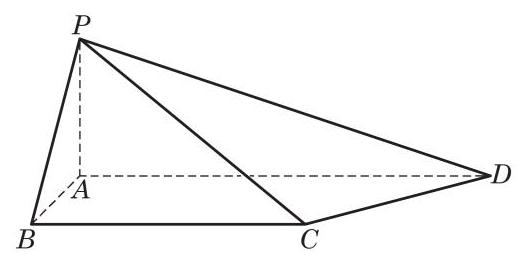
\includegraphics[max width=0.4\textwidth]{images/bo_d7fqvdc91nqc7381i9u0_134_355_316_520_261_0.jpg}
\end{center}
\hspace*{3em} 

(第 8 题)

\begin{center}
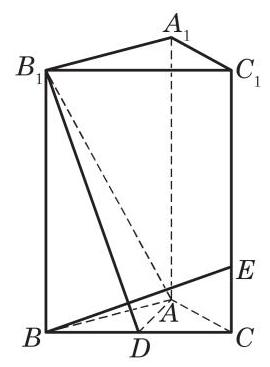
\includegraphics[max width=0.2\textwidth]{images/bo_d7fqvdc91nqc7381i9u0_134_1059_214_270_367_0.jpg}
\end{center}
\hspace*{3em} 

(第 9 题)

9. 如图,在直三棱柱 \({ABC} - {A}_{1}{B}_{1}{C}_{1}\) 中, \(\angle {BAC} = {90}^{ \circ  },\left| {AB}\right|  = \left| {AC}\right|  = a,\left| {A{A}_{1}}\right|  = {2a}\) , \(D\) 为 \({BC}\) 的中点， \(E\) 为 \(C{C}_{1}\) 上的点，且 \(\left| {CE}\right|  = \frac{1}{4}\left| {C{C}_{1}}\right|\) .

(1)求证: \({BE}\bot\) 平面 \({AD}{B}_{1}\) ；

(2)求二面角 \(B - A{B}_{1} - D\) 的大小.

B 组

1. 在长方体 \({ABCD} - {A}_{1}{B}_{1}{C}_{1}{D}_{1}\) 中, \(\left| {AB}\right|  = \left| {BC}\right|  = 2,{A}_{1}D\) 与 \(B{C}_{1}\) 所成的角为 \(\frac{\pi }{2}\) . 求 \(B{C}_{1}\) 与平面 \(B{B}_{1}{D}_{1}D\) 所成角的大小.

2. 如图,在平行六面体 \({ABCD} - {A}_{1}{B}_{1}{C}_{1}{D}_{1}\) 中,点 \(E\text{ 、 }F\) 分别在 \({B}_{1}B\) 和 \({D}_{1}D\) 上,且 \(\left| {BE}\right|  = \frac{1}{3}\left| {B{B}_{1}}\right| ,\left| {DF}\right|  = \frac{2}{3}\left| {D{D}_{1}}\right| .\)

(1)求证: \(A\) 、 \(E\) 、 \({C}_{1}\) 、 \(F\) 四点共面；

(2)若 \(\overrightarrow{EF} = \lambda \overrightarrow{AB} + \mu \overrightarrow{AD} + \nu \overrightarrow{A{A}_{1}}\) ，求 \(\lambda  + \mu  + \nu\) 的值.

\begin{center}
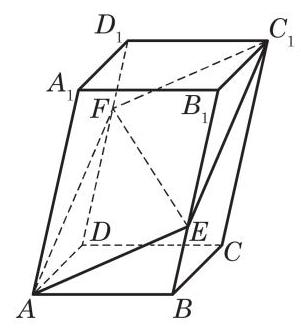
\includegraphics[max width=0.2\textwidth]{images/bo_d7fqvdc91nqc7381i9u0_134_435_1516_301_329_0.jpg}
\end{center}
\hspace*{3em} 

(第 2 题)

\begin{center}
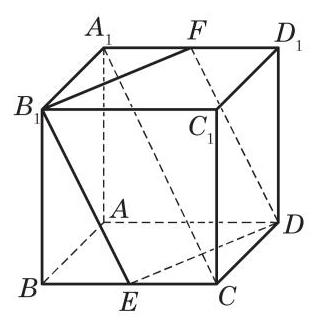
\includegraphics[max width=0.2\textwidth]{images/bo_d7fqvdc91nqc7381i9u0_134_923_1523_313_321_0.jpg}
\end{center}
\hspace*{3em} 

(第 3 题)

3. 如图,在正方体 \({ABCD} - {A}_{1}{B}_{1}{C}_{1}{D}_{1}\) 中, \(E\text{ 、 }F\) 分别是 \({BC}\text{ 、 }{A}_{1}{D}_{1}\) 的中点.

(1)求证:四边形 \({B}_{1}{EDF}\) 是菱形；

(2)求异面直线 \({A}_{1}C\) 与 \({DE}\) 所成角的大小.

4. 在正方体 \({ABCD} - {A}_{1}{B}_{1}{C}_{1}{D}_{1}\) 中, \(E\text{ 、 }F\) 分别是 \({BC}\text{ 、 }C{C}_{1}\) 的中点.

(1)求证:点 \({D}_{1}\) 在平面 \({AEF}\) 上；

(2)求平面 \({AEF}{D}_{1}\) 与底面 \({ABCD}\) 所成二面角的大小.

\section*{拓展与思考}

1. 如图, \({ABCD} - {A}_{1}{B}_{1}{C}_{1}{D}_{1}\) 为正方体,动点 \(P\) 在对角线 \(B{D}_{1}\) 上,记 \(\frac{\left| {D}_{1}P\right| }{\left| {D}_{1}B\right| } = \lambda\) .

(1)求证: \({AP}\bot {B}_{1}C\) ；

(2)若异面直线 \({AP}\) 与 \({D}_{1}{B}_{1}\) 所成角为 \(\frac{\pi }{4}\) ，求 \(\lambda\) 的值；

(3)当 \(\angle {APC}\) 为钝角时,求λ的取值范围.

\begin{center}
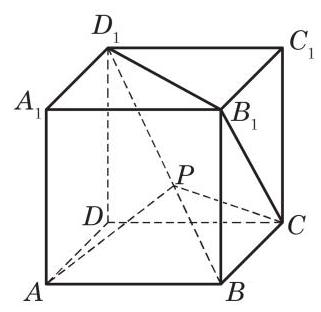
\includegraphics[max width=0.2\textwidth]{images/bo_d7fqvdc91nqc7381i9u0_135_324_783_321_312_0.jpg}
\end{center}
\hspace*{3em} 

(第 1 题)

\begin{center}
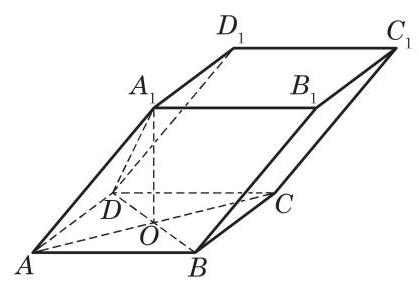
\includegraphics[max width=0.3\textwidth]{images/bo_d7fqvdc91nqc7381i9u0_135_854_801_419_286_0.jpg}
\end{center}
\hspace*{3em} 

(第 2 题)

2. 如图,平行六面体 \({ABCD} - {A}_{1}{B}_{1}{C}_{1}{D}_{1}\) 的底面 \({ABCD}\) 是正方形， \(O\) 为底面的中心， \({A}_{1}O\) 上平面 \({ABCD},\left| {AB}\right|  = \left| {A{A}_{1}}\right|  = \sqrt{2}\) .

(1)求证: \({A}_{1}C\bot\) 平面 \(B{B}_{1}{D}_{1}D\) ；

(2)求平面 \({OC}{B}_{1}\) 与平面 \(B{B}_{1}{D}_{1}D\) 所成二面角的大小.

第 4 章数列

\begin{center}
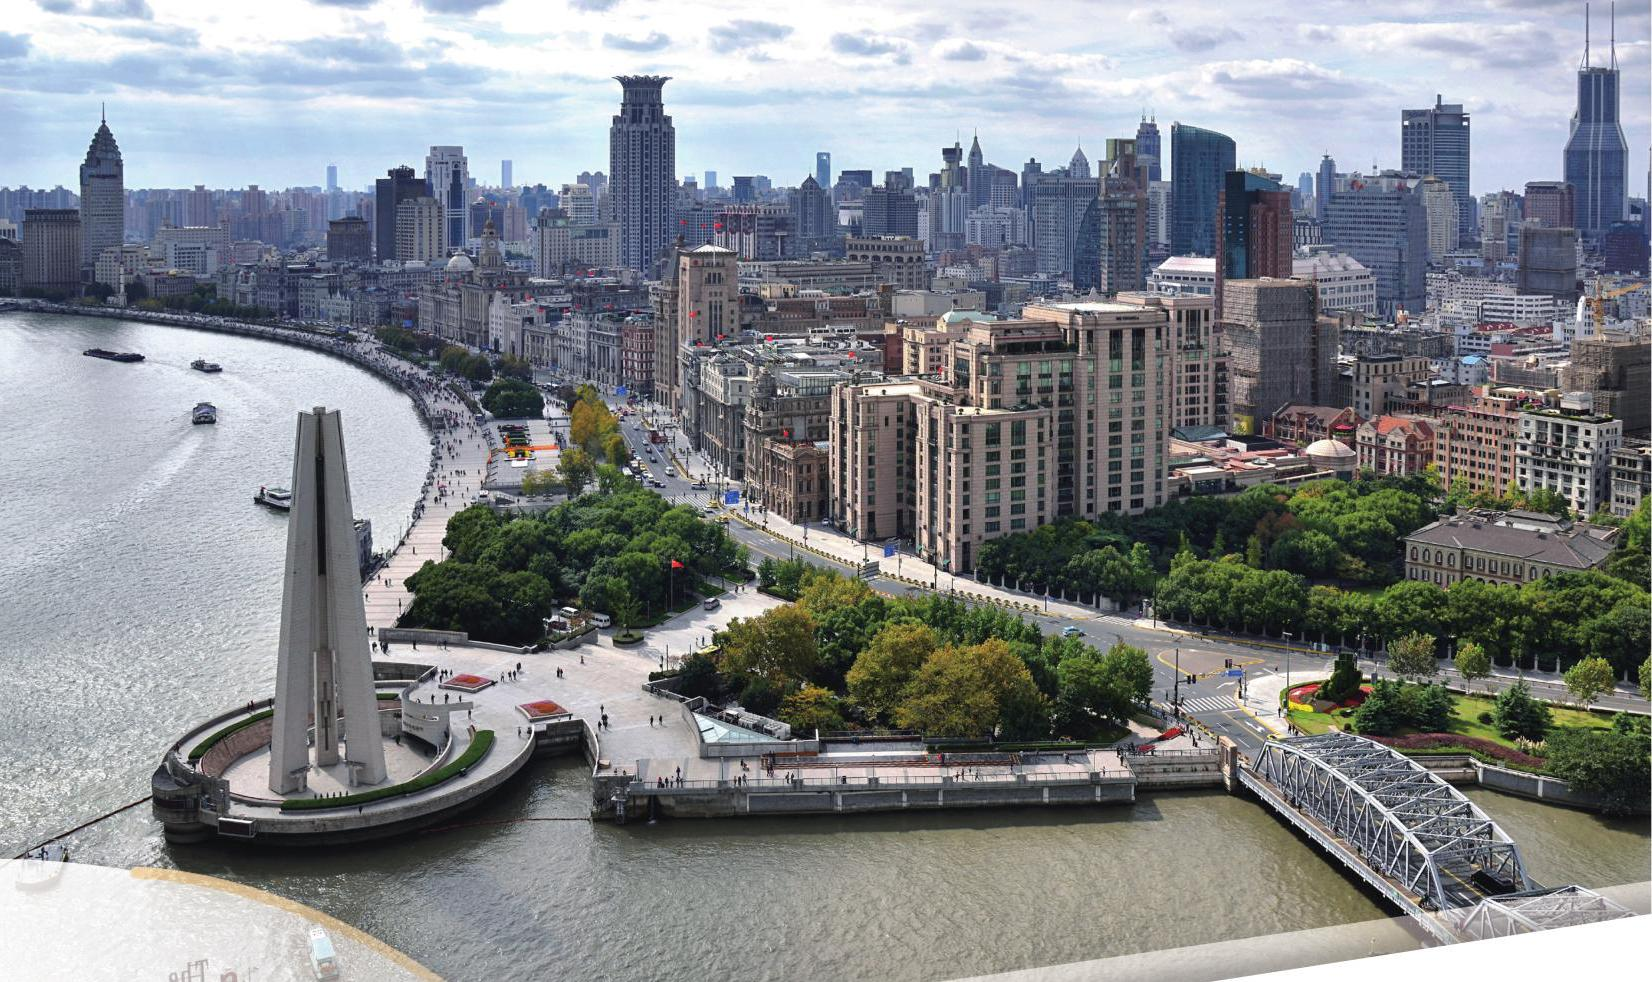
\includegraphics[max width=1.0\textwidth]{images/bo_d7fqvdc91nqc7381i9u0_137_2_0_1652_982_0.jpg}
\end{center}
\hspace*{3em} 

对数列的研究是基于现实生产、生活的需要. 例如, 在若干离散的时间节点, 记录某种数量的变化, 并按时间先后顺序排列起来就得到一个数列. 数列是一个重要的数学概念, 上至一个国家每年的国内生产总值 (GDP), 下至一个人每年的身高或体重，都可以用数列表示. 数列也是学习微积分的一个必要的基础. 本章采用从特殊到一般、从具体到抽象的方法, 先研究两类特殊的数列——等差数列和等比数列, 再在此基础上研究一般的数列. 同时, 介绍数学归纳法这一与数列有关的重要方法, 并通过给出一个利用迭代序列求平方根的方法, 揭示算法在求近似解中的重要作用.

\section*{4.1 等差数列}

\section*{1 等差数列及其通项公式}

在现实生活中, 我们经常见到按一定顺序排列起来的一列数, 称之为数列. 我们将数列中的每一个数叫做这个数列的项. 排在第一位的数称为这个数列的第 1 项 (通常叫做首项), 排在第二位的数称为这个数列的第 2 项, \(\cdots \cdots\) ,排在第 \(n\) 位的数称为这个数列的第 \(n\) 项,等等.

数列的一般形式可以记成

\[
{a}_{1},{a}_{2},{a}_{3},\cdots ,{a}_{n},\cdots ,
\]

其中 \({a}_{n}\) 是数列的第 \(n\) 项,下标 \(n\) 是 \({a}_{n}\) 的序数. 上面的数列常简记为 \(\left\{  {a}_{n}\right\}\) .

观察以下数列, 看它们有什么共同的特点.

(1)月历(图 4-1-1)最后一列数依次为:

3, 10, 17, 24, 31. \circled{1} 

\begin{center}
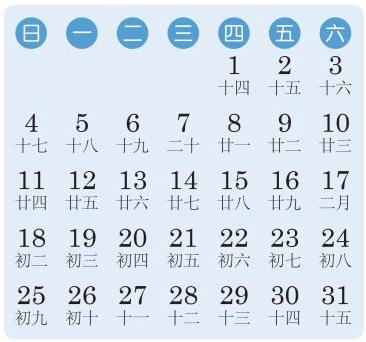
\includegraphics[max width=0.3\textwidth]{images/bo_d7fqvdc91nqc7381i9u0_138_560_1445_366_342_0.jpg}
\end{center}
\hspace*{3em} 

图 4-1-1

\begin{center}
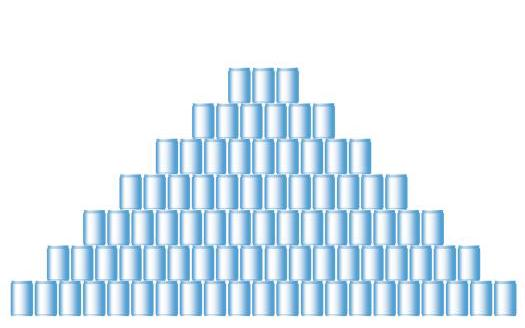
\includegraphics[max width=0.4\textwidth]{images/bo_d7fqvdc91nqc7381i9u0_138_960_1459_525_328_0.jpg}
\end{center}
\hspace*{3em} 

图 4-1-2

(2)按一定规律堆放在一起的食品罐头(图 4-1-2)，共堆放 7 层, 从下到上各层的罐头数依次为:

\[
{21},{18},{15},{12},9,6,3.
\]
  \circled{2} 

(3)全国统一的鞋号中，常见的成年女鞋的尺寸(单位:cm) 由小至大依次为:

\[
{22.5},{23},{23.5},{24},{24.5},{25},{25.5},{26}.
\]
  \circled{3} 

可以看到, 对于数列 \circled{1} , 从第 2 项起, 每一项与其前一项的差都等于 7; 对于数列 \circled{2} , 从第 2 项起, 每一项与其前一项的差都等于 -3 ; 对于数列 \circled{3} ，从第 2 项起，每一项与其前一项的差都等于 0.5 .

这些数列有一个共同特点: 从第 2 项起, 每一项与其前一项的差都等于同一个常数.

定义 如果一个数列从第 2 项起, 每一项与其前一项的差都等于同一个常数, 这个数列就叫做等差数列 (arithmetic sequence), 而这个常数叫做等差数列的公差 (common difference). 公差通常用小写字母 \(d\) 表示.

给定一个数列 \(a,A,b\) . 若 \(a,A,b\) 是等差数列,由定义可得 \(A - a = b - A\) ,从而 \(A = \frac{a + b}{2}\) . 反之,若 \(A = \frac{a + b}{2}\) ,则 \({2A} = a + b\) ,即 \(A - a = b - A\) ,从而 \(a,A,b\) 成等差数列.

这时, \(A\) 叫做 \(a\) 与 \(b\) 的等差中项.

如果等差数列 \(\left\{  {a}_{n}\right\}\) 的首项为 \({a}_{1}\) ,公差为 \(d\) ,由定义可得

\[
{a}_{n} - {a}_{n - 1} = d\left( {n \geq  2}\right) ,
\]

从而

\[
{a}_{2} - {a}_{1} = d,
\]

\[
{a}_{3} - {a}_{2} = d,
\]

\[
{a}_{4} - {a}_{3} = d,
\]

...

\[
{a}_{n} - {a}_{n - 1} = d\left( {n \geq  2}\right) .
\]

把这 \(\left( {n - 1}\right)\) 个等式相加得

\[
{a}_{n} - {a}_{1} = \left( {n - 1}\right) d,
\]

由此

\[
{a}_{n} = {a}_{1} + \left( {n - 1}\right) d\left( {n \geq  2}\right) .
\]

当 \(n = 1\) 时,容易验证上面的等式也成立. 因此,当 \(n\) 为正整数时,等差数列 \(\left\{  {a}_{n}\right\}\) 的第 \(n\) 项可以用如下公式表示:

\[
{a}_{n} = {a}_{1} + \left( {n - 1}\right) d.
\]

像这种用数列的序数 \(n\) 表示相应项 \({a}_{n}\) 的公式称为数列 \(\left\{  {a}_{n}\right\}\) 的通项公式. 而上式就是等差数列 \(\left\{  {a}_{n}\right\}\) 的通项公式.

\HRule

由三个数组成的等差数列可以看成最简单的等差数列.

\HRule

例 1 已知等差数列 \(- 5, - 9, - {13},\cdots\) .

(1)求该等差数列的第 20 项；

(2)一401 是不是该等差数列的项？如果是，指明是第几项; 如果不是,请说明理由.

解 设该等差数列为 \(\left\{  {a}_{n}\right\}\) ,由 \({a}_{1} =  - 5,{a}_{2} =  - 9\) ,得该等差数列的公差 \(d =  - 9 - \left( {-5}\right)  =  - 4\) . 由等差数列的通项公式,得

\[
{a}_{n} =  - 5 - 4\left( {n - 1}\right)  =  - {4n} - 1.
\]

(1)由上述通项公式可得, 该等差数列的第 20 项为

\[
{a}_{20} =  - 4 \times  {20} - 1 =  - {81}.
\]

(2)假设 -401 是这个等差数列中的第 \(n\) 项，则有

\[
- {401} =  - {4n} - 1,
\]

解得

\[
n = {100}\text{ . }
\]

所以, -401 是这个等差数列的第 100 项.

例 2 假设体育场一角看台的座位从第 2 排起每一排都比前一排多相等数目的座位. 若第 3 排有 10 个座位, 第 9 排有 28 个座位, 则第 12 排有多少个座位?

解 由题意可知,体育场该角看台每排的座位数成等差数列,设该数列为 \(\left\{  {a}_{n}\right\}\) ,其公差为 \(d\) ,则 \({a}_{3} = {10},{a}_{9} = {28}\) . 由等差数列的通项公式, 得

\[
\left\{  \begin{array}{l} {a}_{1} + {2d} = {10}, \\  {a}_{1} + {8d} = {28}, \end{array}\right.
\]

解得

\[
\left\{  \begin{array}{l} {a}_{1} = 4, \\  d = 3. \end{array}\right.
\]

所以, \({a}_{12} = 4 + \left( {{12} - 1}\right)  \times  3 = {37}\) .

答: 体育场该角看台的第 12 排有 37 个座位.

例 3 已知 \({a}_{n} = {pn} + q\) 是数列 \(\left\{  {a}_{n}\right\}\) 的通项公式,其中 \(p\) 和 \(q\) 均为常数. 试判断数列 \(\left\{  {a}_{n}\right\}\) 是否为等差数列,并证明你的结论.

分析 为了判断 \(\left\{  {a}_{n}\right\}\) 是否为等差数列,可以利用等差数列的定义,只要判断 \({a}_{n} - {a}_{n - 1}\left( {n \geq  2}\right)\) 的值是否为一个与 \(n\) 无关的常数即可.

解 任取数列 \(\left\{  {a}_{n}\right\}\) 中的相邻两项 \({a}_{n}\) 与 \({a}_{n - 1}\left( {n \geq  2}\right)\) ,求差得

\[
{a}_{n} - {a}_{n - 1} = \left( {{pn} + q}\right)  - \left\lbrack  {p\left( {n - 1}\right)  + q}\right\rbrack   = p\left( {n \geq  2}\right) .
\]

因为 \(p\) 是一个与 \(n\) 无关的常数,所以 \(\left\{  {a}_{n}\right\}\) 是一个等差数列.

\section*{练习 4.1(1)}

1. 下列数列中成等差数列的是 ( )

A.0,1,3,5,7;

B. \(1,\frac{1}{3},\frac{1}{5},\frac{1}{7},\frac{1}{9}\) ;

C. \(1,\sqrt{2},\sqrt{3},2,\sqrt{5}\) ;

D. \(1,\frac{1}{3}, - \frac{1}{3}, - 1, - \frac{5}{3}\) .

2. 设数列 \(\left\{  {a}_{n}\right\}\) 为等差数列,其公差为 \(d\) .

(1)已知 \({a}_{1} =  - 1,d = 4\) ，求 \({a}_{8}\) ；

(2)已知 \({a}_{7} = 8,d =  - \frac{1}{3}\) ，求 \({a}_{1}\) ；

(3)已知 \({a}_{1} = 9,d =  - 2,{a}_{n} =  - {15}\) ，求 \(n\) .

3. 已知数列 \(\left\{  {a}_{n}\right\}\) 是等差数列,正整数 \(m\text{ 、 }n\text{ 、 }p\text{ 、 }q\) 满足 \(m + n = p + q\) . 求证: \({a}_{m} + {a}_{n} = \; {a}_{p} + {a}_{q}.\)

\section*{2 等差数列的前 \(n\) 项和}

\HRule

\begin{center}
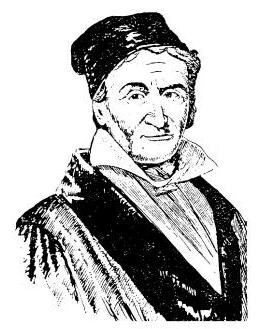
\includegraphics[max width=0.2\textwidth]{images/bo_d7fqvdc91nqc7381i9u0_141_1173_1311_256_329_0.jpg}
\end{center}
\hspace*{3em} 

高斯 (C. F. Gauss, 1777—1855) 德国数学家. 研究的内容涉及数学的诸多领域, 并对天文学和大地测量学的研究有突出贡献. 他在世界上享有崇高的声望，被誉为 “数学王子”.

\HRule

据说 200 多年前, 著名数学家高斯的算术老师在课堂上曾经提出了下面的问题:

求 \(1 + 2 + 3 + \cdots  + {100}\) 的值.

少年高斯用下面的方法迅速算出了正确的答案:

\[
1 + 2 + 3 + \cdots  + {100} = ?
\]

\[
{100} + {99} + {98} + \cdots  + 1 = ?
\]

上述两式相加得: \({101} + {101} + {101} + \cdots  + {101} = 2 \times\) ?

所以，结果为 \(\frac{{101} \times  {100}}{2} = {5050}\) .

高斯的计算方法实际上解决了求等差数列 \(1,2,3,\cdots\) , \(n,\cdots\) 前 100 项和的问题.

事实上, 古代的中国人和希腊人也是这么求等差数列之和的. 例如, 宋朝数学家杨辉提出了一个问题: “今有圭垛草一堆, 顶上一束，底阔八束. 问共几束？答:36 束. ”他的计算方法可以用图 4-1-3 表示.

\begin{center}
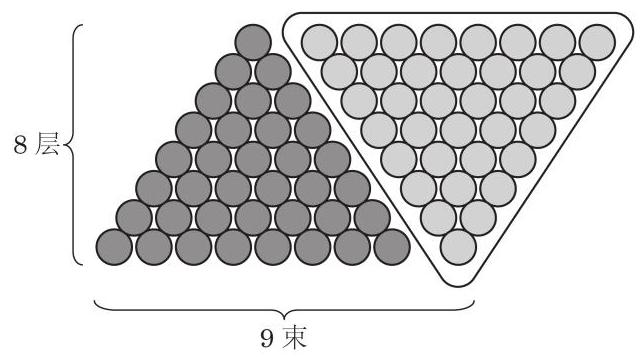
\includegraphics[max width=0.5\textwidth]{images/bo_d7fqvdc91nqc7381i9u0_142_708_245_641_358_0.jpg}
\end{center}
\hspace*{3em} 

图 4-1-3

一般地,将数列 \(\left\{  {a}_{n}\right\}\) 的前 \(n\) 项和记作 \({S}_{n}\) ,即

\[
{S}_{n} = {a}_{1} + {a}_{2} + \cdots  + {a}_{n} = \mathop{\sum }\limits_{{i = 1}}^{n}{a}_{i}.
\]

根据等差数列的通项公式, 上式可以写为

\[
{S}_{n} = {a}_{1} + \left( {{a}_{1} + d}\right)  + \cdots  + \left\lbrack  {{a}_{1} + \left( {n - 2}\right) d}\right\rbrack   + \left\lbrack  {{a}_{1} + \left( {n - 1}\right) d}\right\rbrack  \text{ .  \circled{1}  }
\]

受高斯算法的启示,我们又可将 \({S}_{n}\) 表示为

\[
{S}_{n} = {a}_{n} + {a}_{n - 1} + \cdots  + {a}_{2} + {a}_{1}
\]

\[
= {a}_{n} + \left( {{a}_{n} - d}\right)  + \cdots  + \left\lbrack  {{a}_{n} - \left( {n - 2}\right) d}\right\rbrack   + \left\lbrack  {{a}_{n} - \left( {n - 1}\right) d}\right\rbrack  \text{ .  \circled{2}  }
\]
  \circled{2} 

由 \circled{1} + \circled{2} , 得

\[
2{S}_{n} = \underset{n \uparrow  }{\underbrace{\left( {{a}_{1} + {a}_{n}}\right)  + \left( {{a}_{1} + {a}_{n}}\right)  + \cdots  + \left( {{a}_{1} + {a}_{n}}\right)  + \left( {{a}_{1} + {a}_{n}}\right) }}
\]

\[
= n\left( {{a}_{1} + {a}_{n}}\right) \text{ . }
\]

于是就可得到等差数列 \(\left\{  {a}_{n}\right\}\) 的前 \(n\) 项和公式

\[
{S}_{n} = \frac{n\left( {{a}_{1} + {a}_{n}}\right) }{2}.
\]

由于 \({a}_{n} = {a}_{1} + \left( {n - 1}\right) d\) ,上述公式又可以写作

\[
{S}_{n} = n{a}_{1} + \frac{n\left( {n - 1}\right) }{2}d.
\]

例 4 设数列 \(\left\{  {a}_{n}\right\}\) 为等差数列,其前 \(n\) 项和为 \({S}_{n}\) .

(1)已知 \({a}_{1} = {50},{a}_{8} = {15}\) ，求 \({S}_{8}\) ；

(2)已知 \({a}_{1} = {0.7},{a}_{2} = {1.5}\) ，求 \({S}_{7}\) ；

(3)已知 \({a}_{4} = 7\) ，求 \({S}_{7}\) .

解(1)由等差数列的前 \(n\) 项和公式，得

\[
{S}_{8} = \frac{8 \times  \left( {{50} + {15}}\right) }{2} = {260}.
\]

\HRule

特别地 \(1 + 2 + 3 + \cdots  + n = \frac{n\left( {n + 1}\right) }{2}.\)

\HRule

(2)设公差为 \(d\) ，则 \(d = {a}_{2} - {a}_{1} = {0.8}\) ，于是由等差数列的前 \(n\) 项和公式,有

\[
{S}_{7} = 7 \times  {0.7} + \frac{7 \times  6}{2} \times  {0.8} = {21.7}.
\]

(3)设公差为 \(d\) ，则 \({a}_{1} = {a}_{4} - {3d},{a}_{7} = {a}_{4} + {3d}\) . 从而

\[
{S}_{7} = \frac{7\left( {{a}_{1} + {a}_{7}}\right) }{2} = \frac{7\left\lbrack  {\left( {{a}_{4} - {3d}}\right)  + \left( {{a}_{4} + {3d}}\right) }\right\rbrack  }{2} = 7{a}_{4} = {49}.
\]

例 5 已知等差数列 \(\left\{  {a}_{n}\right\}\) 的前 10 项和 \({S}_{10} = {310}\) ,前 20 项和 \({S}_{20} = {1220}\) ,由此可以确定数列 \(\left\{  {a}_{n}\right\}\) 前 30 项和 \({S}_{30}\) 吗?

解 设该等差数列 \(\left\{  {a}_{n}\right\}\) 的公差为 \(d\) . 由等差数列的前 \(n\) 项和公式 \({S}_{n} = n{a}_{1} + \frac{n\left( {n - 1}\right) }{2}d\) ,可得

\[
\left\{  \begin{array}{l} {10}{a}_{1} + {45d} = {310}, \\  {20}{a}_{1} + {190d} = {1220}, \end{array}\right.
\]

解得

\[
\left\{  \begin{array}{l} {a}_{1} = 4, \\  d = 6. \end{array}\right.
\]

所以, \({S}_{30} = {30} \times  4 + \frac{{30} \times  \left( {{30} - 1}\right) }{2} \times  6 = {2730}\) .

例 6 已知数列 \(\left\{  {a}_{n}\right\}\) 的前 \(n\) 项和为 \({S}_{n} = {n}^{2} + {2n}\) .

(1)求数列 \(\left\{  {a}_{n}\right\}\) 的通项公式；

(2)求证:数列 \(\left\{  {a}_{n}\right\}\) 是等差数列.

解(1)当 \(n \geq  2\) 时,

\[
{S}_{n - 1} = {\left( n - 1\right) }^{2} + 2\left( {n - 1}\right) ,
\]

从而

\[
{a}_{n} = {S}_{n} - {S}_{n - 1} = {n}^{2} + {2n} - \left\lbrack  {{\left( n - 1\right) }^{2} + 2\left( {n - 1}\right) }\right\rbrack   = {2n} + 1.
\]

而当 \(n = 1\) 时, \({a}_{1} = {S}_{1} = {1}^{2} + 2 \times  1 = 3\) 亦满足上式.

所以,数列 \(\left\{  {a}_{n}\right\}\) 的通项公式为 \({a}_{n} = {2n} + 1\) .

(2)证明:由(1)中的结果，当 \(n \geq  2\) 时，

\[
{a}_{n - 1} = 2\left( {n - 1}\right)  + 1 = {2n} - 1,
\]

从而

\[
{a}_{n} - {a}_{n - 1} = \left( {{2n} + 1}\right)  - \left( {{2n} - 1}\right)  = 2.
\]

所以，数列 \(\left\{  {a}_{n}\right\}\) 是一个等差数列.

\HRule

如果一个数列 \(\left\{  {a}_{n}\right\}\) 的前 \(n\) 项和为 \({S}_{n} = p{n}^{2} + {qn} + r,\) 其中 \(p\text{ 、 }q\text{ 、 }r\) 均为常数, 这个数列是等差数列吗?

\HRule

\section*{练习 4.1(2)}

1. 计算 \(\mathop{\sum }\limits_{{i = 1}}^{n}{2i}\) .

2. 设数列 \(\left\{  {a}_{n}\right\}\) 为等差数列,其前 \(n\) 项和为 \({S}_{n}\) .

(1)已知 \({a}_{1} =  - 4,{a}_{8} =  - {18}\) ,求 \({S}_{8}\) ;

(2)已知 \({a}_{1} =  - 4,{a}_{12} = {18}\) ，求 \({S}_{15}\) .

3. 已知数列 \(\left\{  {a}_{n}\right\}\) 的前 \(n\) 项和 \({S}_{n} = {n}^{2} - {3n}\) ，求证:数列 \(\left\{  {a}_{n}\right\}\) 是等差数列.

\section*{习题 4.1}

\section*{A 组}

1. 分别求下列两数的等差中项:

(1) \(\frac{8 - \sqrt{2}}{2}\) 与 \(\frac{8 + \sqrt{2}}{2}\) ；\_\_\_\_\_

(2) \({\left( a + b\right) }^{2}\) 与 \({\left( a - b\right) }^{2}\) .

2. 设数列 \(\left\{  {a}_{n}\right\}\) 为等差数列,其公差为 \(d\) .

(1)已知 \({a}_{1} = 2,d = 3\) ,求 \({a}_{10}\) ;

(2)已知 \({a}_{1} = 3,{a}_{n} = {21},d = 2\) ，求 \(n\) ；

(3)已知 \({a}_{1} = {12},{a}_{6} = {27}\) ，求 \(d\) ；

(4)已知 \({a}_{6} = 9,d =  - \frac{1}{2}\) ，求 \({a}_{1}\) .

3. 已知数列 \(\left\{  {a}_{n}\right\}\) 为等差数列,其公差为 \(d\) . 求证: 对任意给定的正整数 \(m\text{ 、 }n\) ,都有 \({a}_{n} = {a}_{m} + \left( {n - m}\right) d.\)

4. 设数列 \(\left\{  {a}_{n}\right\}\) 为等差数列,其公差为 \(d\) .

(1)已知 \({a}_{2} = {31},{a}_{7} = {76}\) ,求 \({a}_{1}\) 及 \(d\) ;

(2)已知 \({a}_{1} + {a}_{6} = {12},{a}_{4} = 7\) ，求 \({a}_{9}\) .

5. 设数列 \(\left\{  {a}_{n}\right\}\) 为等差数列,其公差为 \(d\) ,前 \(n\) 项和为 \({S}_{n}\) .

(1)已知 \({a}_{1} = {20},{a}_{n} = {54},{S}_{n} = {999}\) ,求 \(d\) 及 \(n\) ;

(2)已知 \(d = \frac{1}{3},{S}_{37} = {629}\) ,求 \({a}_{1}\) 及 \({a}_{37}\) ;

(3)已知 \({a}_{1} = \frac{5}{6},d =  - \frac{1}{6},{S}_{n} =  - 5\) ，求 \(n\) 及 \({a}_{n}\) ；

(4)已知 \(d = 2,{a}_{15} =  - {10}\) ，求 \({a}_{1}\) 及 \({S}_{15}\) .

6. 设数列 \(\left\{  {a}_{n}\right\}\) 为等差数列,其前 \(n\) 项和为 \({S}_{n}\) .

(1)已知 \({a}_{6} = {10},{S}_{5} = 5\) ,求 \({S}_{8}\) ;

(2)已知 \({S}_{4} = 2,{S}_{9} =  - 6\) ，求 \({S}_{12}\) .

7. 设数列 \(\left\{  {a}_{n}\right\}\) 为等差数列,其前 \(n\) 项和为 \({S}_{n}\) .

(1)已知 \({a}_{4} + {a}_{14} = 1\) ，求 \({S}_{17}\) ；

(2)已知 \({S}_{21} = {420}\) ，求 \({a}_{11}\) ；

(3)已知 \({a}_{1} + {a}_{2} + {a}_{3} =  - 3,{a}_{18} + {a}_{19} + {a}_{20} = 6\) ，求 \({S}_{20}\) ；

(4)已知 \({S}_{4} = 2,{S}_{8} = 6\) ，求 \({S}_{16}\) .

8. 求证: “ \(\bigtriangleup  {ABC}\) 三个内角的度数可以构成等差数列” 是 “ \(\bigtriangleup  {ABC}\) 中有一个内角为 \({60}^{ \circ  }\) ”的充要条件.

9.《九章算术》中的“竹九节”问题: 现有一根 9 节的竹子, 自上而下各节的容积成等差数列. 若最上面 4 节的容积共 3 升, 最下面 3 节的容积共 4 升, 则第 5 节的容积为多少升?

\section*{B 组}

1.(1)在等差数列 \(\left\{  {a}_{n}\right\}\) 中，等式 \({a}_{n} = \frac{{a}_{n - 1} + {a}_{n + 1}}{2}\left( {n \geq  2}\right)\) 是否都成立？

(2)在数列 \(\left\{  {a}_{n}\right\}\) 中，如果对于任意的正整数 \(n\left( {n \geq  2}\right)\) ，都有 \({a}_{n} = \frac{{a}_{n - 1} + {a}_{n + 1}}{2}\) ，那么数列 \(\left\{  {a}_{n}\right\}\) 一定是等差数列吗?

2. 在等差数列 \(\left\{  {a}_{n}\right\}\) 中,其前 \(n\) 项和为 \({S}_{n}\) . 已知公差 \(d = 2,{S}_{20} = {400}\) .

(1)写出 \(\mathop{\sum }\limits_{{i = 1}}^{{10}}{a}_{{2i} - 1}\) 的具体展开式，并求其值；

(2)用求和符号表示 \({a}_{2} + {a}_{4} + {a}_{6} + \cdots  + {a}_{20}\) ，并求其值.

3. 在等差数列 \(\left\{  {a}_{n}\right\}\) 中,已知 \({a}_{1} =  - 3,{11}{a}_{5} = 5{a}_{8}\) . 求数列 \(\left\{  {a}_{n}\right\}\) 的前 \(n\) 项和 \({S}_{n}\) 的最小值.

4. 已知等差数列 \(\left\{  {a}_{n}\right\}\) ,其前 \(n\) 项和为 \({S}_{n}\) . 若存在两个不相等的正整数 \(p\) 和 \(q\) ,满足 \({S}_{p} = q,{S}_{q} = p\) ,求 \({S}_{p + q}\) .

5. 已知一个凸多边形各个内角的度数可以排列成一个公差为 5 的等差数列, 且最小角为 \({120}^{ \circ  }\) ,该多边形是几边形?

6. 某产品按质量分成 10 个档次, 生产最低档次产品的利润是 8 元/件. 每提高一个档次, 每件产品的利润增加 2 元, 但产量每天减少 3 件. 如果在某段时间内, 最低档次 (记作第 1 档次) 的产品每天可生产 60 件, 那么在该段时间内, 生产第几档次的产品可获得最大利润?

\section*{4.2 等比数列}

\section*{1 等比数列及其通项公式}

观察以下数列, 看这些数列有什么共同特点.

(1)-1 的 1 次幂、 2 次幂、 3 次幂、 4 次幂……依次为

\[
- 1,1, - 1,1,\cdots \text{ . }
\]
  \circled{1} 

(2)科克雪花曲线. 即将一个边长为 1 的等边三角形的每条边三等分, 以中间一段为边向外作等边三角形, 并擦去中间一段, 如图 4-2-1, 如此继续下去得到图形的每条边的长度依次为

\[
1,\frac{1}{3},\frac{1}{9},\frac{1}{27},\cdots
\]
  \circled{2} 

\begin{center}
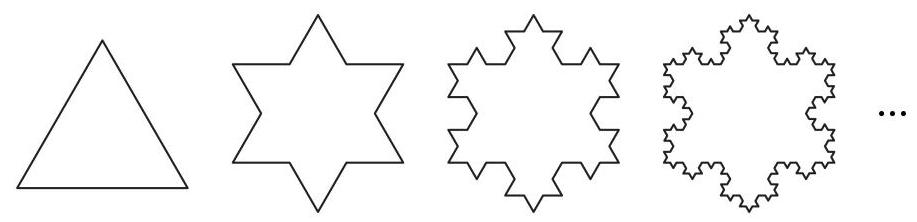
\includegraphics[max width=0.7\textwidth]{images/bo_d7fqvdc91nqc7381i9u0_146_571_1175_917_222_0.jpg}
\end{center}
\hspace*{3em} 

图 4-2-1

(3)图 4-2-1 中的每个图形的边数依次为

\[
3,{12},{48},{192},\cdots \text{ . }
\]
  \circled{3} 

可以看到, 对于数列 \circled{1} , 从第 2 项起, 每一项与其前一项的比都等于 -1 ; 对于数列 \circled{2} , 从第 2 项起, 每一项与其前一项的比都等于 \(\frac{1}{3}\) ; 对于数列 \circled{3} ,从第 2 项起,每一项与其前一项的比都等于 4 .

这些数列有一个共同特点: 从第 2 项起, 每一项与其前一项的比都等于同一个常数.

定义 如果一个数列从第 2 项起, 每一项与其前一项的比都等于同一个非零常数, 这个数列就叫做等比数列 (geometric sequence), 而这个常数叫做等比数列的公比(common ratio). 公比通常用小写字母 \(q\left( {q \neq  0}\right)\) 表示.

\HRule

既是等差数列又是等比数列的数列存在吗? 如果存在, 你能举出例子吗?

\HRule

在两个非零实数 \(a\) 与 \(b\) 中间插入一个数 \(G\) ,使 \(a,G,b\) 成等比数列. 根据等比数列的定义,有 \(\frac{G}{a} = \frac{b}{G}\) ,从而 \({G}^{2} = {ab}\) ,即 \(G = \sqrt{ab}\) 或 \(G =  - \sqrt{ab}\) . 这两种情形下, \(a,G,b\) 均为等比数列. 此时, \(G\) 叫做 \(a\) 与 \(b\) 的等比中项.

根据等比数列的定义,以 \({a}_{1}\) 为首项、以 \(q\) 为公比的等比数列 \(\left\{  {a}_{n}\right\}\) 满足 \(\frac{{a}_{n}}{{a}_{n - 1}} = q\left( {n \geq  2}\right)\) . 因此,当 \(n \geq  2\) 时,有

\[
\frac{{a}_{2}}{{a}_{1}} = q,\frac{{a}_{3}}{{a}_{2}} = q,\frac{{a}_{4}}{{a}_{3}} = q,\cdots ,\frac{{a}_{n}}{{a}_{n - 1}} = q.
\]

由此可得, \(\frac{{a}_{n}}{{a}_{1}} = {q}^{n - 1}\) . 所以, \({a}_{n} = {a}_{1}{q}^{n - 1}\left( {n \geq  2}\right)\) . 而当 \(n = 1\) 时, 上面的等式也显然成立.

因此,当 \(n\) 为正整数时,等比数列 \(\left\{  {a}_{n}\right\}\) 的第 \(n\) 项可表示为

\[
{a}_{n} = {a}_{1}{q}^{n - 1}.
\]

这称为等比数列 \(\left\{  {a}_{n}\right\}\) 的通项公式.

例 1 设数列 \(\left\{  {a}_{n}\right\}\) 为等比数列.

(1)已知 \({a}_{1} = 3\) ，公比 \(q =  - 2\) ，求 \({a}_{6}\) ；

(2)已知 \({a}_{3} = {20},{a}_{6} = {160}\) ，求 \({a}_{n}\) .

解(1)由等比数列的通项公式，得

\[
{a}_{6} = 3 \times  {\left( -2\right) }^{6 - 1} =  - {96}.
\]

(2)设等比数列 \(\left\{  {a}_{n}\right\}\) 的公比为 \(q\) ，那么

\[
\left\{  \begin{array}{l} {a}_{1}{q}^{2} = {20}, \\  {a}_{1}{q}^{5} = {160}. \end{array}\right.
\]

解得

\[
\left\{  \begin{array}{l} {a}_{1} = 5, \\  q = 2. \end{array}\right.
\]

所以, \({a}_{n} = {a}_{1}{q}^{n - 1} = 5 \times  {2}^{n - 1}\) .

例 2 某种放射性物质不断衰变为其他物质, 设每经过一年剩余的这种放射性物质是年初的 84\%. 这种放射性物质的半衰期约为多少?(结果精确到 1 年)

解 设这种物质最初的质量是 1,而经过 \(n\) 年,剩余量是 \({a}_{n}\) .

由条件可知,数列 \(\left\{  {a}_{n}\right\}\) 是一个等比数列,且 \({a}_{1} = {0.84}\) , 公比 \(q = {0.84}\) . 当 \({a}_{n} = {0.5}\) 时,则 \({0.84}^{n} = {0.5}\) .

在上式两边同时取以 10 为底的对数, 并求解得

\[
n = \frac{\lg {0.5}}{\lg {0.84}} \approx  4.
\]

答: 这种物质的半衰期大约为 4 年.

例 3 (1)已知 \(a,b,c\) 成等差数列，其公差为 \(d\) . 试证明 \({3}^{a},{3}^{b},{3}^{c}\) 成等比数列,并写出其公比.

(2)已知正实数 \(a,b,c\) 成等比数列，其公比为 \(q\) . 试证明 \(\lg a,\lg b,\lg c\) 成等差数列,并写出其公差.

解(1)因为 \(a,b,c\) 成等差数列，所以 \({2b} = a + c\) . 从而

\[
{3}^{2b} = {3}^{a + c} = {3}^{a} \cdot  {3}^{c},
\]

所以， \({3}^{a}\) ， \({3}^{b}\) ， \({3}^{c}\) 成等比数列，其公比为 \(\frac{{3}^{b}}{{3}^{a}} = {3}^{b - a} = {3}^{d}\) .

(2)因为正实数 \(a,b,c\) 成等比数列，所以 \({b}^{2} = {ac}\) . 在上式两边同时取以 10 为底的对数, 得

\[
2\lg b = \lg a + \lg c,
\]

所以, \(\lg a,\lg b,\lg c\) 成等差数列,其公差为 \(\lg b - \lg a = \lg \frac{b}{a} = \lg q\) .

\section*{练习 4.2(1)}

1. 下列数列中成等比数列的是 ( )

A. \(1,\frac{1}{4},\frac{1}{9},\frac{1}{16}\) ; B. \(1,1, - 1, - 1\) ;

C. \(1,\frac{\sqrt{2}}{2},\frac{1}{2},\frac{\sqrt{2}}{4}\) ; D. \(\frac{1}{2},2,\frac{1}{2},2\) .

2. 设数列 \(\left\{  {a}_{n}\right\}\) 为等比数列,其公比为 \(q\) .

(1)已知 \({a}_{1} =  - 3,q = 2\) ,求 \({a}_{5}\) ;

(2)已知 \({a}_{1} = 1,q = 2,{a}_{n} = {16}\) ,求 \(n\) ;

(3)已知 \({a}_{1} = \frac{1}{3},{a}_{7} = 9\) ，求 \(q\) ；

(4)已知 \(q =  - \frac{3}{2},{a}_{4} =  - {27}\) ，求 \({a}_{1}\) .

3. 已知数列 \(\left\{  {a}_{n}\right\}\) 是等比数列,正整数 \(m\text{ 、 }n\text{ 、 }s\text{ 、 }t\) 满足 \(m + n = s + t\) . 求证: \({a}_{m} \cdot  {a}_{n} =\)

\section*{2 等比数列的前 \(n\) 项和}

国际象棋起源于古代印度. 发明者将棋盘划分为 8 行 8 列, 构成 64 个方格. 相传国王要奖励该发明者, 问他有什么要求. 发明者说: “请在棋盘的第 1 个格子里放上 1 颗麦粒, 在第 2 个格子里放上 2 颗麦粒, 在第 3 个格子里放上 4 颗麦粒，依次类推，每个格子里放的麦粒数都是前一个格子里放的麦粒数的 2 倍, 直到放完 64 个格子为止. 请给我足够的麦粒以实现上述要求. ”这位发明者要了多少颗麦粒？国王能实现他的要求吗?

\begin{center}
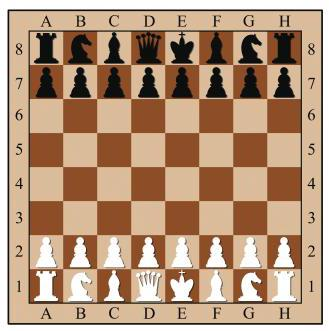
\includegraphics[max width=0.2\textwidth]{images/bo_d7fqvdc91nqc7381i9u0_149_1144_560_329_331_0.jpg}
\end{center}
\hspace*{3em} 

这实际上是求以 1 为首项、以 2 为公比的等比数列的前 64 项的和:

\[
{S}_{64} = 1 + 2 + {2}^{2} + \cdots  + {2}^{62} + {2}^{63}.
\]

如果用公比 2 乘上述等式的两边, 就得到

\[
2{S}_{64} = 2 + {2}^{2} + {2}^{3}\cdots  + {2}^{63} + {2}^{64}.
\]

可以发现, 上面两式中有许多相同的项, 两式相减可以消去这些项, 得到

\[
{S}_{64} = {2}^{64} - 1.
\]

这是一个二十位数, 将这些小麦折算成质量 (每千粒麦子的质量设为 \({40}\mathrm{\;g}\) ),会超过 7000 亿吨. 即使到小麦年产量比较高的现代，全世界小麦年总产量也远低于 10 亿吨，国王根本满足不了发明者的要求.

一般地,设等比数列 \(\left\{  {a}_{n}\right\}\) 的公比为 \(q\) ,其前 \(n\) 项和为

\[
{S}_{n} = {a}_{1} + {a}_{1}q + {a}_{1}{q}^{2} + \cdots  + {a}_{1}{q}^{n - 1}.
\]

将上式两边同乘公比 \(q\) ,可得

\[
q{S}_{n} = {a}_{1}q + {a}_{1}{q}^{2} + {a}_{1}{q}^{3} + \cdots  + {a}_{1}{q}^{n}.
\]

将两式相减, 可得

\[
{S}_{n} - q{S}_{n} = {a}_{1} - {a}_{1}{q}^{n},
\]

即

\[
\left( {1 - q}\right) {S}_{n} = {a}_{1}\left( {1 - {q}^{n}}\right) .
\]

由此得到,当 \(q \neq  1\) 时,等比数列 \(\left\{  {a}_{n}\right\}\) 的前 \(n\) 项和为

\[
{S}_{n} = \frac{{a}_{1}\left( {1 - {q}^{n}}\right) }{1 - q}.
\]

综上所述,可以得到以 \({a}_{1}\) 为首项、以 \(q\left( {q \neq  1}\right)\) 为公比的等比数列的前 \(n\) 项和公式为

\[
{S}_{n} = \frac{{a}_{1}\left( {1 - {q}^{n}}\right) }{1 - q}\left( {q \neq  1}\right) .
\]

因为 \({a}_{n} = {a}_{1}{q}^{n - 1}\) ,所以上式又可写为

\[
{S}_{n} = \frac{{a}_{1} - {a}_{n}q}{1 - q}\left( {q \neq  1}\right) .
\]

而当 \(q = 1\) 时,因为 \({a}_{1} = {a}_{2} = \cdots  = {a}_{n}\) ,所以 \({S}_{n} = n{a}_{1}\) .

例 4 设数列 \(\left\{  {a}_{n}\right\}\) 为等比数列,其前 \(n\) 项和为 \({S}_{n}\) .

(1)已知 \({a}_{1} =  - 4\) ，公比 \(q =  - \frac{1}{2}\) ，求 \({S}_{10}\) ；

(2)已知 \({a}_{1} = {27},{a}_{n} = \frac{1}{243}\) ，公比 \(q =  - \frac{1}{3}\) ，求 \({S}_{n}\) .

解 (1) 根据等比数列的前 \(n\) 项和公式,得

\[
{S}_{10} = \frac{-4 \times  \left\lbrack  {1 - {\left( -\frac{1}{2}\right) }^{10}}\right\rbrack  }{1 - \left( {-\frac{1}{2}}\right) } =  - \frac{341}{128}.
\]

(2)根据等比数列的前 \(n\) 项和公式，得

\[
{S}_{n} = \frac{{a}_{1} - {a}_{n}q}{1 - q} = \frac{{27} - \frac{1}{243} \times  \left( {-\frac{1}{3}}\right) }{1 - \left( {-\frac{1}{3}}\right) } = \frac{4921}{243}.
\]

例 5 在等比数列 \(\left\{  {a}_{n}\right\}\) 中,其前 \(n\) 项和为 \({S}_{n}\) . 已知 \({S}_{3} = \frac{7}{2}\) , \({S}_{6} = \frac{63}{2}\) ,求 \({a}_{n}\) .

解 设该等比数列的公比为 \(q\) . 若 \(q = 1\) ,则 \({S}_{6} = 2{S}_{3}\) . 这与已知条件矛盾,所以 \(q \neq  1\) . 从而有

\[
{S}_{3} = \frac{{a}_{1}\left( {1 - {q}^{3}}\right) }{1 - q} = \frac{7}{2},
\]

\[
{S}_{6} = \frac{{a}_{1}\left( {1 - {q}^{6}}\right) }{1 - q} = \frac{63}{2},
\]

将上面两个等式相除, 得

\[
1 + {q}^{3} = 9.
\]

于是 \(q = 2\) ,从而由上面关于 \({S}_{3}\) 的式子就可得 \({a}_{1} = \frac{1}{2}\) ,因此

\[
{a}_{n} = \frac{1}{2} \times  {2}^{n - 1} = {2}^{n - 2}.
\]

\HRule

若数列 \(\left\{  {a}_{n}\right\}\) 的前 \(n\) 项和为 \({S}_{n} = A{q}^{n} + B \; \left( {q \neq  0,1}\right)\) ,当 \(A\text{ 、 }B\) 满足什么条件时, 数列 \(\left\{  {a}_{n}\right\}\) 是等比数列?

\HRule

例 6 已知数列 \(\left\{  {a}_{n}\right\}\) 的前 \(n\) 项和为 \({S}_{n} = {3}^{n} + a\) . 当常数 \(a\) 满足什么条件时,数列 \(\left\{  {a}_{n}\right\}\) 是等比数列?

解 当 \(n = 1\) 时,可得 \({a}_{1} = {S}_{1} = 3 + a\) . 而当 \(n \geq  2\) 时,

\[
{a}_{n} = {S}_{n} - {S}_{n - 1} = \left( {{3}^{n} + a}\right)  - \left( {{3}^{n - 1} + a}\right)  = 2 \times  {3}^{n - 1}.
\]

从而

\[
\frac{{a}_{n + 1}}{{a}_{n}} = \frac{2 \times  {3}^{n}}{2 \times  {3}^{n - 1}} = 3,n \geq  2.
\]

于是,当且仅当 \(\frac{{a}_{2}}{{a}_{1}} = 3\) 时,数列 \(\left\{  {a}_{n}\right\}\) 是等比数列. 由上式, \({a}_{1} = 3 + a,\) 而 \({a}_{2} = 6\) ,由 \(\frac{{a}_{2}}{{a}_{1}} = 3\) ,解得 \(a =  - 1\) .

因此,当 \(a =  - 1\) 时,数列 \(\left\{  {a}_{n}\right\}\) 是等比数列.

\section*{练习 4.2(2)}

1. 设数列 \(\left\{  {a}_{n}\right\}\) 为等比数列,其前 \(n\) 项和为 \({S}_{n}\) .

(1)已知 \({a}_{1} = 3\) ，公比 \(q = 2\) ，求 \({S}_{6}\) ；

(2)已知 \({a}_{1} =  - {2.7}\) ，公比 \(q =  - \frac{1}{3}\) ， \({a}_{n} = \frac{1}{90}\) ，求 \({S}_{n}\) .

2. 已知等比数列 \(\left\{  {a}_{n}\right\}\) 的前 5 项和为 10,前 10 项和为 50 . 求这个数列的前 15 项和.

3. 中国古代数学著作《算法统宗》中有这样一个问题: “三百七十八里关，初行健步不为难，次日脚痛减一半，六朝才得到其关，要见次日行里数，请公仔细算相还.”其意思为:有一个人要走 378 里路，第一天健步行走，从第二天起因为脚痛，每天走的路程为前一天的一半, 走了 6 天后到达目的地. 请问第二天走了多少里.

中国古代庄周所著的《庄子·天下篇》说:“一尺之棰，日取其半, 万世不竭. ”其含义是: 一根一尺长的木棒, 每天截取其一半, 这样的过程可以无限进行下去. 如果从第一天开始截取, 把木棒每天剩余的长度记录下来, 可得到下面一个数列:

\[
\frac{1}{2},\frac{1}{4},\frac{1}{8},\frac{1}{16},\cdots ,{\left( \frac{1}{2}\right) }^{n},\cdots .
\]

随着 \(n\) 无限增大,此数列的第 \(n\) 项 \({a}_{n} = {\left( \frac{1}{2}\right) }^{n}\) 的值越来越趋近于零,从而 \({a}_{n}\) 的极限为零. 记作 \(\mathop{\lim }\limits_{{n \rightarrow   + \infty }}{a}_{n} = 0\) .

上述数列的前 \(n\) 项之和为

\[
{S}_{n} = \frac{1}{2} + \frac{1}{4} + \frac{1}{8} + \cdots  + {\left( \frac{1}{2}\right) }^{n}
\]

\[
= \frac{\frac{1}{2}\left\lbrack  {1 - {\left( \frac{1}{2}\right) }^{n}}\right\rbrack  }{1 - \frac{1}{2}}
\]

\[
= 1 - {\left( \frac{1}{2}\right) }^{n}\text{ . }
\]

随着 \(n\) 无限增大, \({\left( \frac{1}{2}\right) }^{n}\) 的值越来越趋近于零, \({S}_{n}\) 的值越来越趋近于 1,从而 \({S}_{n}\) 的极限为 1,记作 \(\mathop{\lim }\limits_{{n \rightarrow   + \infty }}{S}_{n} = 1\) .

更一般地,对于首项为 \(a\) 、公比为 \(q\) 的等比数列:

\[
{a}_{n} = a{q}^{n - 1}\text{ ( }n\text{ 为正整数), }
\]

当 \(0 < \left| q\right|  < 1\) 时,此数列的前 \(n\) 项和为

\[
{S}_{n} = a + {aq} + \cdots  + a{q}^{n - 1}
\]

\[
= \frac{a}{1 - q}\left( {1 - {q}^{n}}\right) .
\]

随着 \(n\) 无限增大, \({q}^{n}\) 的值越来越趋近于零, \({S}_{n}\) 的值越来越趋近于 \(\frac{a}{1 - q}\) ,从而 \({S}_{n}\) 的极限为 \(\frac{a}{1 - q}\) ,记作 \(\mathop{\lim }\limits_{{n \rightarrow   + \infty }}{S}_{n} = \frac{a}{1 - q}\) .

Q

综上所述，以 \(a\) 为首项、 \(q\) 为公比的等比数列，当公比 \(0 < \; \left| q\right|  < 1\) 时,有

\[
\mathop{\sum }\limits_{{i = 1}}^{{+\infty }}a{q}^{i - 1} = \frac{a}{1 - q}.
\]

例 7 化下列循环小数为分数:

(1) \(0.\dot{29}\) ; (2) \({0.4}\dot{31}\) .

Q

解 (1) \({0.29} = {0.29} + {0.29} \times  {0.01} + {0.29} \times  {\left( {0.01}\right) }^{2} + \cdots  + \; {0.29} \times  {\left( {0.01}\right) }^{n - 1} + \cdots .\)

相应的无穷等比数列是 \({0.29},{0.29} \times  {0.01},{0.29} \times  {\left( {0.01}\right) }^{2},\cdots\) , \({0.29} \times  {\left( {0.01}\right) }^{n - 1},\cdots\) ,其首项是 0.29,公比是 0.01,于是有

\[
{0.29} = \frac{0.29}{1 - {0.01}} = \frac{29}{99}.
\]

\HRule

一个数列 \(\left\{  {a}_{n}\right\}\) 中, 如果当 \(n\) 无限增大时, \({a}_{n}\) 的值越来越趋近于某个确定的数 \(a\) ,那么称这个数列的极限为 \(a\) ,记作 \(\mathop{\lim }\limits_{{n \rightarrow   + \infty }}{a}_{n} = a\) , 其中记号 \(\lim\) 是英文单词 limit (极限) 的缩写.

如果一个数列 \(\left\{  {a}_{n}\right\}\) 的前 \(n\) 项和为 \({S}_{n}\) ,则 \(\mathop{\sum }\limits_{{i = 1}}^{{+\infty }}{a}_{i}\) 表示 \(\mathop{\lim }\limits_{{n \rightarrow   + \infty }}{S}_{n}\) .

类似地, 我们可以证明: \(0.\dot{9} = 1\) .

\HRule

(2) \({0.43}\dot{1} = {0.4} + {0.031} + {0.031} \times  {0.01} + {0.031} \times  {\left( {0.01}\right) }^{2} + \cdots  + \; {0.031} \times  {\left( {0.01}\right) }^{n - 1} + \cdots\) .

上述等式的右边除 0.4 外,相应的无穷等比数列是 \({0.031},{0.031} \times \; {0.01},{0.031} \times  {\left( {0.01}\right) }^{2},\cdots ,{0.031} \times  {\left( {0.01}\right) }^{n - 1},\cdots\) ,其首项是 0.031 , 公比是 0.01 , 于是有

\[
{0.431} = {0.4} + \frac{0.031}{1 - {0.01}} = \frac{4}{10} + \frac{31}{990} = \frac{427}{990}.
\]

例 8 如图 4-2-2,正方形 \({ABCD}\) 的边长等于 1,连接这个正方形各边的中点得到一个小正方形 \({A}_{1}{B}_{1}{C}_{1}{D}_{1}\) ; 又连接正方形 \({A}_{1}{B}_{1}{C}_{1}{D}_{1}\) 各边的中点得到一个更小的正方形 \({A}_{2}{B}_{2}{C}_{2}{D}_{2}\) ; 如此无限继续下去. 求所有这些正方形的周长的和与面积的和.

\begin{center}
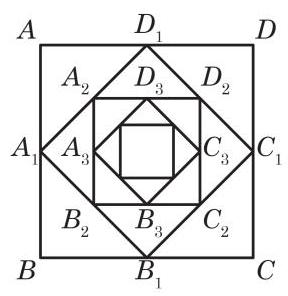
\includegraphics[max width=0.2\textwidth]{images/bo_d7fqvdc91nqc7381i9u0_153_1135_723_288_296_0.jpg}
\end{center}
\hspace*{3em} 

图 4-2-2

解 由题设,可得到第 1 个正方形的边长 \({a}_{1} = 1\) ,第 2 个正方形的边长 \({a}_{2} = \frac{\sqrt{2}}{2},\cdots \cdots ,\) 第 \(n\) 个正方形的边长 \({a}_{n} =\)

\[
\sqrt{{\left( \frac{{a}_{n - 1}}{2}\right) }^{2} + {\left( \frac{{a}_{n - 1}}{2}\right) }^{2}} = \frac{\sqrt{2}{a}_{n - 1}}{2}\left( {n \geq  2}\right) .
\]

所有这些正方形的边长组成的数列为

\[
1,\frac{\sqrt{2}}{2},\frac{1}{2},\frac{\sqrt{2}}{4},\cdots ,{\left( \frac{\sqrt{2}}{2}\right) }^{n - 1},\cdots ,
\]

从而所有这些正方形的周长组成的数列为

\[
4,2\sqrt{2},2,\sqrt{2},\cdots ,4 \cdot  {\left( \frac{\sqrt{2}}{2}\right) }^{n - 1},\cdots .
\]

这是一个以 4 为首项、以 \(\frac{\sqrt{2}}{2}\) 为公比的等比数列,因此所有这些正方形的周长的和为

\[
\mathop{\sum }\limits_{{i = 1}}^{{+\infty }}4 \cdot  {\left( \frac{\sqrt{2}}{2}\right) }^{i - 1} = \frac{4}{1 - \frac{\sqrt{2}}{2}} = 8 + 4\sqrt{2}.
\]

所有这些正方形的面积组成的数列为

\[
1,\frac{1}{2},\frac{1}{4},\frac{1}{8},\cdots ,{\left( \frac{1}{2}\right) }^{n - 1},\cdots .
\]

这是以 1 为首项、以 \(\frac{1}{2}\) 为公比的等比数列,因此所有这些正方形

的面积的和为

\[
\mathop{\sum }\limits_{{i = 1}}^{{+\infty }}{\left( \frac{1}{2}\right) }^{i - 1} = \frac{1}{1 - \frac{1}{2}} = 2.
\]

\section*{练习 4.2(3)}

1. 计算 \(\mathop{\sum }\limits_{{i = 1}}^{{+\infty }}{\left( \frac{1}{3}\right) }^{i}\) .

2. 化下列循环小数为分数:

(1)0.13 ；

\begin{center}
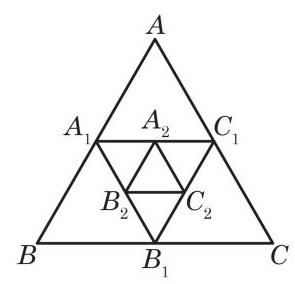
\includegraphics[max width=0.2\textwidth]{images/bo_d7fqvdc91nqc7381i9u0_154_1204_781_295_284_0.jpg}
\end{center}
\hspace*{3em} 

(第 3 题)

(2)1.332.

3. 如图,已知等边三角形 \({ABC}\) 的面积等于 1,连接这个三角形各边的中点得到一个小的三角形 \({A}_{1}{B}_{1}{C}_{1}\) ,又连接三角形 \({A}_{1}{B}_{1}{C}_{1}\) 各边的中点得到一个更小的三角形 \({A}_{2}{B}_{2}{C}_{2}\) ,这样的过程可以无限继续下去. 求所有三角形 \({A}_{i}{B}_{i}{C}_{i}\left( {i = 1,2,3,\cdots }\right)\) 的面积的和.

\section*{习题 4.2}

\section*{A 组}

1. 求下列各组数的等比中项:

(1) \(\sqrt{3} + 1\) 与 \(\sqrt{3} - 1\) ；

(2) \({a}^{4} + {a}^{2}{b}^{2}\) 与 \({b}^{4} + {a}^{2}{b}^{2}\left( {a \neq  0,b \neq  0}\right)\) .

2. 设数列 \(\left\{  {a}_{n}\right\}\) 为等比数列,其公比为 \(q\) .

(1)已知 \({a}_{5} = 8,{a}_{8} = 1\) ,求 \({a}_{1}\text{ 、 }q\) ;

(2)已知 \({a}_{3} = 2,q =  - 1\) ，求 \({a}_{15}\) ；

(3)已知 \({a}_{4} = {12},{a}_{8} = 6\) ，求 \({a}_{12}\) .

3. 已知数列 \(\left\{  {a}_{n}\right\}\) 为等比数列,其公比为 \(q\) . 判断下列数列是否为等比数列. 如果是, 求其公比; 如果不是, 请说明理由.

(1)数列 \(\left\{  {2{a}_{n}}\right\}\) ；

(2)数列 \(\left\{  {{a}_{n} + {a}_{n + 1}}\right\}\) .

4. 已知数列 \(\left\{  {a}_{n}\right\}\) 和数列 \(\left\{  {b}_{n}\right\}\) 为项数相同的等比数列,公比分别为 \({q}_{1}\) 和 \({q}_{2}\) . 求证: 数列 \(\left\{  {{a}_{n}{b}_{n}}\right\}\) 为等比数列,其公比为 \({q}_{1}{q}_{2}\) .

5. 已知直角三角形的斜边长为 \(c\) ,两条直角边长分别为 \(a\) 和 \(b\left( {a < b}\right)\) ,且 \(a,b,c\) 成等比数列. 求 \(a : c\) 的值.

6. 某产品经过 4 次革新后, 成本由原来的 105 元下降到 60 元. 如果这种产品每次革新后成本下降的百分比相同，那么每次革新后成本下降的百分比是多少？(结果精确到 0.1\%)

7. 设数列 \(\left\{  {a}_{n}\right\}\) 为等比数列,其公比为 \(q\) ,前 \(n\) 项和为 \({S}_{n}\) .

(1)已知 \({a}_{1} = 5,q = 3\) ，求 \({S}_{5}\) ；

(2)已知 \({a}_{8} = \frac{1}{16},q = \frac{1}{2}\) ,求 \({S}_{8}\) ；

(3)已知 \({a}_{1} =  - 2,q =  - \frac{1}{2},{a}_{n} = \frac{1}{1024}\) ,求 \({S}_{n}\) ;

(4)已知 \({S}_{6} = \frac{189}{4},q = \frac{1}{2}\) ，求 \({a}_{1}\) .

8. 设等比数列 \(\left\{  {a}_{n}\right\}\) 的公比 \(q < 1\) ,前 \(n\) 项和为 \({S}_{n}\) . 已知 \({a}_{3} = 2,{S}_{4} = 5{S}_{2}\) ,求数列 \(\left\{  {a}_{n}\right\}\) 的通项公式.

9. 一个球从 \({100}\mathrm{\;m}\) 高处自由落下,假设每次着地后又跳回到原高度的一半再落下.

(1)当它第 10 次着地时，求它经过的总路程；

(2)它可能在某次着地时，经过的总路程超过 \({300}\mathrm{\;m}\) 吗？如果可能，请说明是第几次着地首次超过 \({300}\mathrm{\;m}\) ；如果不可能，请说明理由.

B 组

1. 已知 \(b\) 是 \(a\) 与 \(c\) 的等比中项,且 \(a\text{ 、 }b\text{ 、 }c\) 同号. 求证: \(\frac{a + b + c}{3},\sqrt{\frac{{ab} + {bc} + {ca}}{3}}\) , \(\sqrt[3]{abc}\) 成等比数列.

2. 已知 \(a \neq  b\) ,且 \(a\text{ 、 }b\) 都不为 0 . 设 \(n\) 为正整数,写出 \(\mathop{\sum }\limits_{{i = 0}}^{n}{a}^{n - i}{b}^{i}\) 的具体展开式,并证明 \(\mathop{\sum }\limits_{{i = 0}}^{n}{a}^{n - i}{b}^{i} = \frac{{a}^{n + 1} - {b}^{n + 1}}{a - b}\) .

3. 已知对任意给定的正整数 \(n\) ,数列 \(\left\{  {a}_{n}\right\}\) 的前 \(n\) 项和 \({S}_{n} = \frac{1 - {q}^{n}}{1 - q}\left( {q \neq  0\text{ 且 }q \neq  1}\right)\) . 判断 \(\left\{  {a}_{n}\right\}\) 是否为等比数列,并说明理由.

4. 已知数列 \(\left\{  {a}_{n}\right\}\) 为等差数列,数列 \(\left\{  {b}_{n}\right\}\) 满足 \({b}_{n} = {\left( \frac{1}{2}\right) }^{{a}_{n}}\) ( \(n\) 为正整数).

(1)求证:数列 \(\left\{  {b}_{n}\right\}\) 为等比数列；

(2)若 \({b}_{1} + {b}_{2} + {b}_{3} = \frac{21}{8},{b}_{1}{b}_{2}{b}_{3} = \frac{1}{8}\) ，求数列 \(\left\{  {a}_{n}\right\}\) 的通项公式.

5. 如图,已知直角三角形 \({AOB}\) 的两条直角边 \({AO}\) 和 \({BO}\) 的长分别为 5 和 12,点 \({O}_{1}\text{ 、 }{O}_{2}\text{ 、 }\cdots \text{ 、 }{O}_{n}\text{ 、 }\cdots\) 在边 \({OB}\) 上,半圆 \({O}_{1}\) 与 \({AO}\) 和 \({AB}\) 所在直线均相切,半圆 \({O}_{2}\text{ 、 }{O}_{3}\text{ 、 }\cdots \text{ 、 }{O}_{n}\text{ 、 }\cdots\) 与 \({AB}\) 所在直线相切,且与半圆 \({O}_{1}\text{ 、 }{O}_{2}\text{ 、 }\cdots \text{ 、 }{O}_{n - 1}\text{ 、 }\cdots\) 分别外切. 设这些半圆的半径分别为 \({r}_{1}\text{ 、 }{r}_{2}\text{ 、 }\cdots \text{ 、 }{r}_{n}\text{ 、 }\cdots\) .

\begin{center}
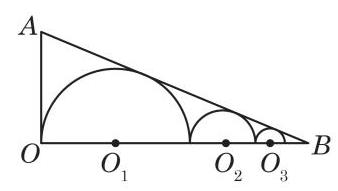
\includegraphics[max width=0.2\textwidth]{images/bo_d7fqvdc91nqc7381i9u0_156_1159_228_338_191_0.jpg}
\end{center}
\hspace*{3em} 

(第 5 题)

(1)求证:数列 \(\left\{  {r}_{n}\right\}\) 为等比数列；

(2)求前 \(n\) 个半圆弧长的总和 \({L}_{n}\) ；

(3)利用前 \(n\) 个半圆弧长的总和 \({L}_{n}\) 的表达式,计算 \(\mathop{\lim }\limits_{{n \rightarrow   + \infty }}{L}_{n}\) .

\section*{4.3 数列}

\section*{1 数列的概念与性质}

除了我们前面学过的等差数列、等比数列这两类特殊的数列外, 在现实世界中, 许多事物的数量也可以排成一列数.

(1)如图 4-3-1，能够表示成三角形点阵的点数依次为

\[
1,3,6,{10},{15},{21},{28},\cdots \text{ . }
\]
  \circled{1} 

\begin{center}
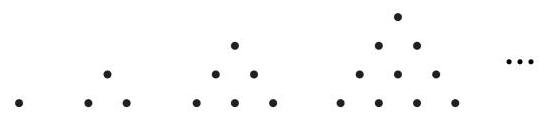
\includegraphics[max width=0.4\textwidth]{images/bo_d7fqvdc91nqc7381i9u0_157_357_985_548_121_0.jpg}
\end{center}
\hspace*{3em} 

图 4-3-1

(2)如图 4-3-2，能够表示成正方形点阵的点数依次为

\[
1,4,9,{16},{25},\cdots \text{ . }
\]
  \circled{2} 

\begin{center}
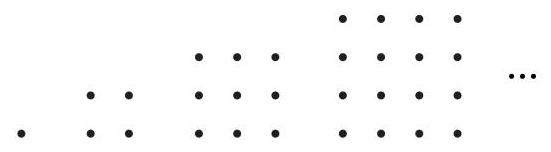
\includegraphics[max width=0.4\textwidth]{images/bo_d7fqvdc91nqc7381i9u0_157_354_1364_551_152_0.jpg}
\end{center}
\hspace*{3em} 

图 4-3-2

(3)目前通用的第五套人民币纸币的面额(单位:元)按照从大到小的顺序排列依次为

\[
{100},{50},{20},{10},5,1.
\]
  \circled{3} 

(4)医生要对病人的体温进行 24 小时监控，某天从 0 时开始记录，每隔 4 小时记录一次，共记录 7 次，监测到病人的体温 (单位:℃)依次为 Q

\[
{39.2},{38.3},{37.5},{37.0},{36.8},{37.2},{37.6}\text{ . }
\]
  \circled{4} 

(5)将 \(\sqrt{2}\) 的不足近似值按小数位数从少到多的顺序排列依次为

\[
1,{1.4},{1.41},{1.414},{1.4142},{1.41421},\cdots \text{ . }
\]
  \circled{5} 

\HRule

\(\sqrt{2}\) 的不足近似值: 按照所需要的精确度截取指定数位后, 直接略去后面的数位, 就得到了一个小于 \(\sqrt{2}\) 的近似值,称为 \(\sqrt{2}\) 的不足近似值.

\HRule

像这样, 按照一定顺序排列的一列数称为一个数列 (number sequence). 数列与以往学过的数集相比, 有下述不同点: 集合中的元素是无序的, 而数列的项必须按一定顺序排列, 即为有序的; 此外, 集合中的元素要求互异, 而数列的项可以是相同的.

给定一个数列 \(\left\{  {a}_{n}\right\}\) ,当项的序数 \(n\) 确定时,相应的项 \({a}_{n}\) 也就确定了. 于是,项 \({a}_{n}\) 与项的序数 \(n\) 之间存在着对应关系,这种对应关系可描述如下

\begin{center}
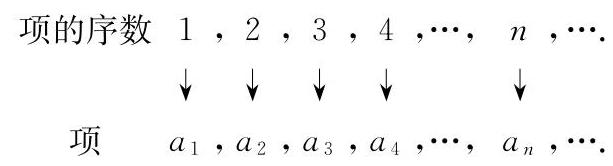
\includegraphics[max width=0.5\textwidth]{images/bo_d7fqvdc91nqc7381i9u0_158_723_715_613_166_0.jpg}
\end{center}
\hspace*{3em} 

项数有限的数列叫做有穷数列 (finite sequence); 项数无限的数列叫做无穷数列 (infinite sequence). 从第 2 项起, 每一项都不小于其前一项的数列 \(\left\{  {a}_{n}\right\}\) 叫做增数列,此时 \({a}_{n + 1} \geq  {a}_{n}\) ( \(n\) 为正整数)成立. 特别地，从第 2 项起,每一项都大于其前一项的数列 \(\left\{  {a}_{n}\right\}\) 叫做严格增数列,此时 \({a}_{n + 1} > {a}_{n}\) ( \(n\) 为正整数) 成立. 相应地,从第 2 项起,每一项都不大于其前一项的数列 \(\left\{  {a}_{n}\right\}\) 叫做减数列,此时 \({a}_{n + 1} \leq  {a}_{n}\) ( \(n\) 为正整数) 成立. 特别地,从第 2 项起,每一项都小于其前一项的数列 \(\left\{  {a}_{n}\right\}\) 叫做严格减数列,此时 \({a}_{n + 1} < {a}_{n}\) ( \(n\) 为正整数) 成立. 增数列和减数列统称为单调数列. 各项均相等的数列叫做常数列.

给定数列 \(\left\{  {a}_{n}\right\}\) ,如果可以用一个关于序数 \(n\) 的公式来表示数列中的任一项 \({a}_{n}\) ,那么这个公式就称为数列 \(\left\{  {a}_{n}\right\}\) 的通项公式 (general term). 有了数列的通项公式, 就可以算出数列中的各项.

实际中, 也常用列表法来表示数列. 例如, 对于数列 \circled{4} , 我们可以用下表直观地表示:

表 4-1

\begin{center}
\adjustbox{max width=\textwidth}{
\begin{tabular}{|c|c|c|c|c|c|c|c|}
\hline
监测序数 \(\left( n\right)\) & 1 & 2 & 3 & 4 & 5 & 6 & 7 \\
\cline{1-8}
体温 \(\left( {a}_{n}\right)\) & 39.2 & 38.3 & 37.5 & 37.0 & 36.8 & 37.2 & 37.6 \\
\cline{1-8}
\hline
\end{tabular}
}
\end{center}

注:体温单位为℃ (摄氏度).

\HRule

公差为正数的等差数列为严格增数列; 公差为负数的等差数列为严格减数列; 公差为零的等差数列为常数列.

\HRule

例 1 已知数列 \(\left\{  {a}_{n}\right\}\) 的通项公式,写出这些数列的前 5 项:

(1) \({a}_{n} = \frac{n - 2}{n + 1}\) ;

(2) \({a}_{n} = 1 + {\left( -\frac{1}{2}\right) }^{n}\) .

解 我们可根据相应的通项公式, 用列表法分别写出这两个数列的前 5 项.

表 4-2

\begin{center}
\adjustbox{max width=\textwidth}{
\begin{tabular}{|c|c|c|c|c|c|}
\hline
\(n\) & 1 & 2 & 3 & 4 & 5 \\
\cline{1-6}
\({a}_{n} = \frac{n - 2}{n + 1}\) & \(- \frac{1}{2}\) & 0 & \(\frac{1}{4}\) & 2 5 & \(\frac{1}{2}\) \\
\cline{1-6}
\({a}_{n} = 1 + {\left( -\frac{1}{2}\right) }^{n}\) & \(\frac{1}{2}\) & 5 & 7 8 & 17 16 & 31 \\
\cline{1-6}
\hline
\end{tabular}
}
\end{center}

例 2 给出数列 \(\left\{  {a}_{n}\right\}\) 的下述通项公式,判断这些数列是否为单调数列, 请说明理由.

(1) \({a}_{n} = 1 + {\left( \frac{1}{2}\right) }^{n}\) ；

(2) \({a}_{n} = n - \frac{1}{n}\) .

解( 1 )因为

\[
{a}_{n + 1} - {a}_{n} = \left\lbrack  {1 + {\left( \frac{1}{2}\right) }^{n + 1}}\right\rbrack   - \left\lbrack  {1 + {\left( \frac{1}{2}\right) }^{n}}\right\rbrack
\]

\[
=  - {\left( \frac{1}{2}\right) }^{n + 1} < 0,
\]

所以 \({a}_{n + 1} < {a}_{n}\) . 因此数列 \(\left\{  {a}_{n}\right\}\) 为严格减数列,从而是单调数列.

(2)因为

\[
{a}_{n + 1} - {a}_{n} = \left( {n + 1 - \frac{1}{n + 1}}\right)  - \left( {n - \frac{1}{n}}\right)
\]

\[
= 1 + \frac{1}{n\left( {n + 1}\right) } > 0,
\]

所以 \({a}_{n + 1} > {a}_{n}\) . 因此数列 \(\left\{  {a}_{n}\right\}\) 为严格增数列,从而是单调数列.

例 3 已知数列 \(\left\{  {a}_{n}\right\}\) 的通项公式是 \({a}_{n} = \left( {n + 1}\right) {\left( \frac{9}{10}\right) }^{n - 1}\) . 试问: 该数列是否有最大项? 若有, 指出第几项最大; 若没有, 试说明理由.

解 因为

\[
{a}_{n + 1} - {a}_{n} = \left( {n + 2}\right) {\left( \frac{9}{10}\right) }^{n} - \left( {n + 1}\right) {\left( \frac{9}{10}\right) }^{n - 1}
\]

\[
= {\left( \frac{9}{10}\right) }^{n - 1} \cdot  \left( \frac{8 - n}{10}\right) ,
\]

所以当 \(n \leq  7\) 时， \({a}_{n + 1} > {a}_{n}\) ；当 \(n = 8\) 时， \({a}_{n + 1} = {a}_{n}\) ；当 \(n \geq  9\) 时, \({a}_{n + 1} < {a}_{n}\) .

于是,数列 \(\left\{  {a}_{n}\right\}\) 的最大项为第 8 项和第 9 项,其值为 \(\frac{{9}^{8}}{{10}^{7}}\) .

\section*{练习 4.3(1)}

1. 根据数列 \(\left\{  {a}_{n}\right\}\) 的通项公式填表:

\begin{center}
\adjustbox{max width=\textwidth}{
\begin{tabular}{|c|c|c|c|c|c|c|c|c|c|}
\hline
\(n\) & 1 & 2 & ... & 5 & ... & \phantom{X} & ... & \(n\) & ... \\
\cline{1-10}
\({a}_{n}\) & \phantom{X} & \phantom{X} & ... & \phantom{X} & ... & 156 & ... & \(n\left( {n + 1}\right)\) & ... \\
\cline{1-10}
\hline
\end{tabular}
}
\end{center}

2. 图中的三角形图案称为谢宾斯基三角形. 在下图四个三角形图案中, 着色的小三角形的个数依次排列成一个数列的前四项, 请写出其前四项, 并给出这个数列的一个通项公式.

\begin{center}
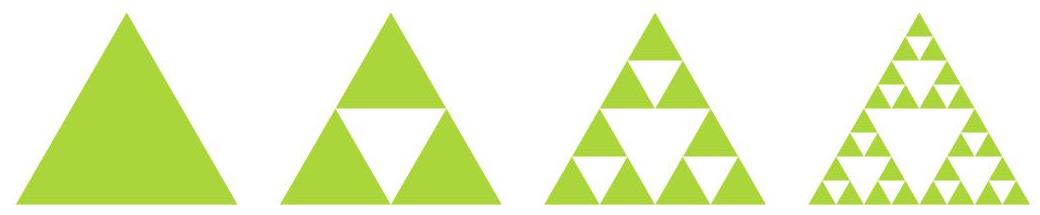
\includegraphics[max width=0.8\textwidth]{images/bo_d7fqvdc91nqc7381i9u0_160_324_1235_1040_215_0.jpg}
\end{center}
\hspace*{3em} 

(第 2 题)

3. 已知数列 \(\left\{  {a}_{n}\right\}\) 的通项公式是 \({a}_{n} = \left| {{2n} - 7}\right|\) . 试问: 该数列是否有最小项? 若有,指出第几项最小; 若没有,试说明理由.

\section*{2 数列的递推公式}

等差数列 \(\left\{  {a}_{n}\right\}\) 满足 \({a}_{1} = 2\) ,公差 \(d = 3\) . 可以用公式

\[
{a}_{n} = {a}_{n - 1} + 3\left( {n \geq  2}\right)
\]

表示该数列从第 2 项起每一项与其前一项的关系.

等比数列 \(\left\{  {a}_{n}\right\}\) 满足 \({a}_{1} = 2\) ,公比 \(q = 3\) . 可以用公式

\[
{a}_{n} = 3{a}_{n - 1}\left( {n \geq  2}\right)
\]

表示该数列从第 2 项起每一项与其前一项的关系.

如果数列 \(\left\{  {a}_{n}\right\}\) 的任一项 \({a}_{n}\) 可由其前一项 \({a}_{n - 1}\) (或前几项) 通过一个公式来表示, 那么这个公式就叫做这个数列的一个递推公式. 它也是表示数列的一种方法. 有时, 数列通项公式不容易被发现, 但可通过数列的递推关系来描述该数列.

例 4 在平面上画 \(n\) 条直线,假设其中任意 2 条直线都相交,且任意 3 条直线都不共点. 设这 \(n\) 条直线将平面分成了 \({a}_{n}\) 个部分.

(1)写出数列 \(\left\{  {a}_{n}\right\}\) 的一个递推公式；

(2)写出数列 \(\left\{  {a}_{n}\right\}\) 的一个通项公式.

解 (1) 我们先通过观察 \(n = 1,2,3\) 时的图形来探究 \({a}_{n}\) 的情况.

\begin{center}
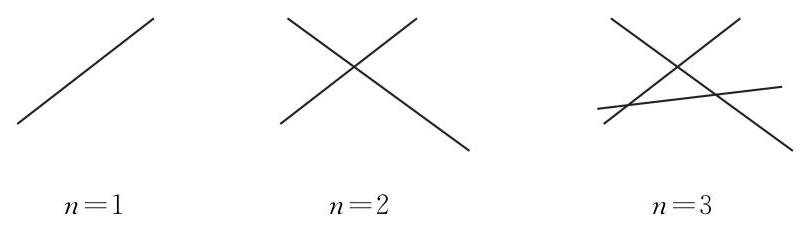
\includegraphics[max width=0.6\textwidth]{images/bo_d7fqvdc91nqc7381i9u0_161_211_992_804_230_0.jpg}
\end{center}
\hspace*{3em} 

图 4-3-3

从图 4-3-3 中可以看出:

当 \(n = 1\) 时,第 1 条直线将平面分为两个部分,所以

\[
{a}_{1} = 2\text{ . }
\]

当 \(n = 2\) 时,第 2 条直线与前面的 1 条直线相交,有 1 个交点. 这个交点将第 2 条直线分成 2 段, 且每一段将原有的平面部分进一步多分出两个部分, 所以

\[
{a}_{2} = {a}_{1} + 2\text{ . }
\]

当 \(n = 3\) 时,第 3 条直线与前面的 2 条直线都相交,有 2 个交点. 这 2 个交点将第 3 条直线分成 3 段, 且每一段将原有的平面部分进一步多分出三个部分, 所以

\[
{a}_{3} = {a}_{2} + 3\text{ . }
\]

依此类推: 第 \(n\left( {n \geq  2}\right)\) 条直线与前面的 \(\left( {n - 1}\right)\) 条直线都相交, 有 \(\left( {n - 1}\right)\) 个交点. 这 \(\left( {n - 1}\right)\) 个交点将第 \(n\) 条直线分成 \(n\) 段,且每一段将原有的平面部分进一步多分出 \(n\) 个部分,所以

\[
{a}_{n} = {a}_{n - 1} + n\;\left( {n \geq  2}\right)
\]

是数列 \(\left\{  {a}_{n}\right\}\) 的递推公式.

(2)由上述递推公式，有

\[
{a}_{2} = {a}_{1} + 2,
\]

\[
{a}_{3} = {a}_{2} + 3,
\]

\[
{a}_{4} = {a}_{3} + 4,
\]

...

\[
{a}_{n} = {a}_{n - 1} + n\left( {n \geq  2}\right) .
\]

由上述等式以及 \({a}_{1} = 2\) ,可得

\[
{a}_{n} = {a}_{1} + 2 + 3 + 4 + \cdots  + n
\]

\[
= {a}_{1} + \frac{\left( {n + 2}\right) \left( {n - 1}\right) }{2}
\]

\[
= \frac{{n}^{2} + n + 2}{2}\;\left( {n \geq  2}\right) .
\]

当 \(n = 1\) 时,由于 \({a}_{1} = 2\) ,上面的等式也成立.

所以,数列 \(\left\{  {a}_{n}\right\}\) 的通项公式为 \({a}_{n} = \frac{{n}^{2} + n + 2}{2}\) .

例 5 已知数列 \(\left\{  {a}_{n}\right\}\) 满足 \({a}_{1} = 1,{a}_{n} = 2{a}_{n - 1} + 1\left( {n \geq  2}\right)\) .

(1)求证:数列 \(\left\{  {{a}_{n} + 1}\right\}\) 为等比数列；

(2)求数列 \(\left\{  {a}_{n}\right\}\) 的通项公式.

解 (1) 证明: 已知递推公式 \({a}_{n} = 2{a}_{n - 1} + 1\left( {n \geq  2}\right)\) .

在上述等式两边同时加 1 , 得

\[
{a}_{n} + 1 = 2{a}_{n - 1} + 2 = 2\left( {{a}_{n - 1} + 1}\right) \left( {n \geq  2}\right) .
\]

由递推公式,易证 \({a}_{n} > 0\left( {n \geq  1}\right)\) ,于是 \({a}_{n - 1} + 1 > 0\left( {n \geq  2}\right)\) , 故 \(\frac{{a}_{n} + 1}{{a}_{n - 1} + 1} = 2\left( {n \geq  2}\right)\) . 所以,数列 \(\left\{  {{a}_{n} + 1}\right\}\) 是以 \({a}_{1} + 1 = 2\) 为首项、以 2 为公比的等比数列.

(2)因为数列 \(\left\{  {{a}_{n} + 1}\right\}\) 是以 \({a}_{1} + 1 = 2\) 为首项、以 2 为公比的等比数列, 所以

\[
{a}_{n} + 1 = {2}^{n}\left( {n \geq  1}\right) ,
\]

从而 \({a}_{n} = {2}^{n} - 1\left( {n \geq  1}\right)\) ,这就是数列 \(\left\{  {a}_{n}\right\}\) 的一个通项公式.

\section*{练习 4.3(2)}

1. 已知数列 \(\left\{  {a}_{n}\right\}\) 对任意正整数 \(n\) ,均满足 \({a}_{1}{a}_{2}\cdots {a}_{n} = {n}^{2}\) .

(1)写出数列 \(\left\{  {a}_{n}\right\}\) 的前五项；

(2)求数列 \(\left\{  {a}_{n}\right\}\) 的通项公式.

2. 在数列 \(\left\{  {a}_{n}\right\}\) 中, \({a}_{1} = 2\) ,且 \({a}_{n} = {a}_{n - 1} + \lg \frac{n}{n - 1}\left( {n \geq  2}\right)\) . 求数列 \(\left\{  {a}_{n}\right\}\) 的通项公式.

3. 已知数列 \(\left\{  {a}_{n}\right\}\) 满足 \({a}_{1} = 1,{a}_{n} = 2{a}_{n - 1} + 3\left( {n \geq  2}\right)\) .

(1)求证:数列 \(\left\{  {{a}_{n} + 3}\right\}\) 为等比数列；

(2)求数列 \(\left\{  {a}_{n}\right\}\) 的通项公式.

\section*{课后阅读}

\section*{神奇的斐波那契数列}

1202 年, 意大利数学家斐波那契 (L. Fibonacci) 出版了一部著作《算盘全书》(Liber Abacci). 他在书中提出了一个关于兔子繁殖的问题: 一对新生的小兔子(一雄一雌)，到第 3 个月开始每月新生一对(一雄一雌)小兔子. 在假设不发生死亡的情况下，问:从第一对新生小兔子开始，到第 10 个月底会有多少对兔子?

第 1 个月, 只有 1 对小兔子; 第 2 个月, 那对小兔子长成熟了; 第 3 个月, 成熟的兔子生下 1 对小兔子, 这时有 2 对兔子; 第 4 个月, 成熟的兔子再生 1 对小兔子, 而另 1 对小兔子长成熟了，共有 3 对兔子；如此推算下去，我们可以得到下面的表格:

表 4-3

\begin{center}
\adjustbox{max width=\textwidth}{
\begin{tabular}{|c|c|c|c|}
\hline
时间/月 & 初生兔子/对 & 成熟兔子/对 & 兔子总数/对 \\
\cline{1-4}
1 & 1 & 0 & 1 \\
\cline{1-4}
2 & 0 & 1 & 1 \\
\cline{1-4}
3 & 1 & 1 & 2 \\
\cline{1-4}
4 & 1 & 2 & 3 \\
\cline{1-4}
5 & 2 & 3 & 5 \\
\cline{1-4}
6 & 3 & 5 & 8 \\
\cline{1-4}
7 & 5 & 8 & 13 \\
\cline{1-4}
8 & 8 & 13 & 21 \\
\cline{1-4}
9 & 13 & 21 & 34 \\
\cline{1-4}
10 & 21 & 34 & 55 \\
\cline{1-4}
\hline
\end{tabular}
}
\end{center}

如果时间不限于 10 个月, 在理想的情境下, 这个问题引出如下的无穷数列:

\(1,1,2,3,5,8,{13},{21},{34},{55},{89},{144},{233},\cdots ,\) 这就是斐波那契数列, 其中的每一个数都称为斐波那契数. 它有这样的特点: 从第三项开始,每一项都是其前两项的和. 如果用 \({F}_{n}\) 表示第 \(n\) 个斐波那契数,那么有

\[
{F}_{n} = {F}_{n - 1} + {F}_{n - 2}\left( {n \geq  3}\right) .
\]

可以证明 (有兴趣的同学, 可查阅有关的课外阅读资料), 其通项公式为

\[
{F}_{n} = \frac{1}{\sqrt{5}}\left\lbrack  {{\left( \frac{1 + \sqrt{5}}{2}\right) }^{n} - {\left( \frac{1 - \sqrt{5}}{2}\right) }^{n}}\right\rbrack  .
\]

人们在研究斐波那契数列的过程中，发现该数列在自然界竟是如此普遍. 例如，考虑树木枝条的数量. 某种树木第 1 年长出幼枝，第 2 年幼枝长成粗干，第 3 年粗干可生出幼枝. 如图 4-3-4, 每条树枝都按照这个规律成长, 则每年的分枝数正好构成斐波那契数列.

\begin{center}
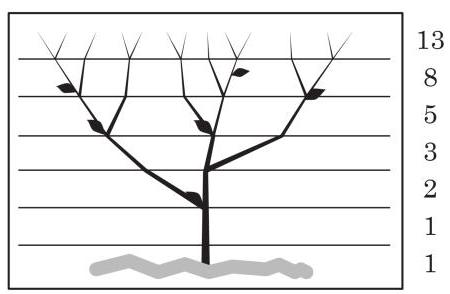
\includegraphics[max width=0.3\textwidth]{images/bo_d7fqvdc91nqc7381i9u0_164_619_768_450_294_0.jpg}
\end{center}
\hspace*{3em} 

图 4-3-4

\HRule

黄金比例又称为黄金分割数, 是指点 \(P\) 把线段 \({AB}\) 分割成 \({AP}\) 和 \({PB}\) 两段,使得 \({AP}\) 是 \({AB}\) 和 \({PB}\) 的比例中项. 其中, \({AP}\) 与 \({AB}\) 的比值 \(\frac{\sqrt{5} - 1}{2}\) 称为黄金比例, 也叫黄金分割数, 它是被公认的最具有审美意义的比例数.

\HRule

在数学上, 斐波那契数列有许多奇妙的性质. 其任一给定项与其后一项的比交替地大于或小于黄金比例, 并且该比值无限趋近于黄金比例, 即有

\[
\mathop{\lim }\limits_{{n \rightarrow   + \infty }}\frac{{F}_{n}}{{F}_{n + 1}} = \frac{\sqrt{5} - 1}{2}.
\]

只要你的心中有“数”，随处可见斐波那契数列. 它蕴含在自然界中, 也出现在文艺作品里. 它是解开不少数学谜题的钥匙, 更在诸多科学领域中有着广泛的应用. 经由斐波那契数列的镜像, 我们的世界竟是如此五彩缤纷!

\section*{习题 4.3}

\section*{A 组}

1. 已知下列数列 \(\left\{  {a}_{n}\right\}\) 的通项公式,写出它的前 4 项.

(1) \({a}_{n} = {n}^{2} - {5n}\) ； (2) \({a}_{n} = \frac{\cos {n\pi }}{2}\) .

2. 已知数列 \(\left\{  {a}_{n}\right\}\) 的通项公式为 \({a}_{n} = \frac{{n}^{2} + n - 1}{3},{79}\frac{2}{3}\) 是否是该数列中的项? 若是,是第几项?

3. 已知数列 \(\left\{  {a}_{n}\right\}\) 的通项公式为 \({a}_{n} = {n}^{2} - {8n} + 5\) .

(1)写出这个数列的前 5 项;

(2)这个数列有没有最小项？如果有，是第几项？

4. 已知数列 \(\left\{  {a}_{n}\right\}\) 的通项公式为 \({a}_{n} = \left( {{3n} - 2}\right) {\left( \frac{3}{5}\right) }^{n}\) ，试问:该数列是否有最大项、最小项? 若有, 分别指出第几项最大、最小; 若没有, 试说明理由.

5. 已知数列 \(\left\{  {a}_{n}\right\}\) 的首项 \({a}_{1} = 1\) ,且 \({a}_{n} = {2}^{n - 1} \cdot  {a}_{n - 1}\left( {n \geq  2}\right)\) . 求数列 \(\left\{  {a}_{n}\right\}\) 的通项公式.

6. 已知数列 \(\left\{  {a}_{n}\right\}\) 满足 \({a}_{1} = {33}\) ,且 \({a}_{n} - {a}_{n - 1} = 2\left( {n - 1}\right) \left( {n \geq  2}\right)\) . 求数列 \(\left\{  \frac{{a}_{n}}{n}\right\}\) 的最小项.

7. 一个正方形被等分成九个相等的小正方形, 将最中间的一个正方形挖掉, 得图 \circled{1} ; 再将剩下的每个正方形都分成九个相等的小正方形, 并将其最中间的一个正方形挖掉, 得图 \circled{2} ; 如此继续下去······

(1)图 \circled{3} 中共挖掉了多少个正方形？

(2)每张图中挖掉的正方形的总数依次组成一个数列，求该数列的一个递推公式.

\begin{center}
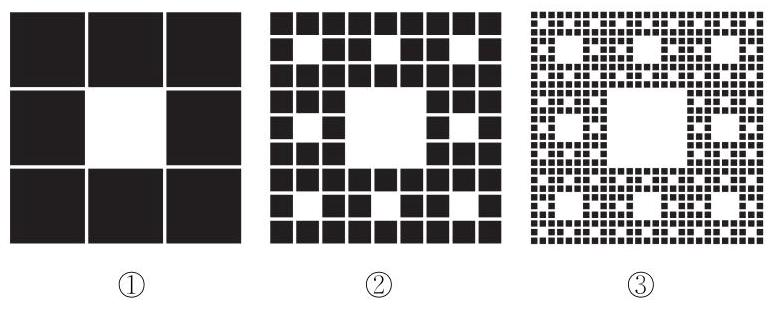
\includegraphics[max width=0.6\textwidth]{images/bo_d7fqvdc91nqc7381i9u0_165_425_1220_773_309_0.jpg}
\end{center}
\hspace*{3em} 

(第 7 题)

B 组

1. 已知数列 \(\left\{  {a}_{n}\right\}\) 的通项公式为 \({a}_{n} = \frac{n - \sqrt{97}}{n - \sqrt{98}}\) ,试问: 该数列是否有最大项、最小项? 若有, 分别指出第几项最大、最小; 若没有, 试说明理由.

2. 已知数列 \(\left\{  {a}_{n}\right\}\) 的通项公式为 \({a}_{n} = {n}^{2} + {\lambda n}\) ,其中 \(\lambda\) 是常数. 若数列 \(\left\{  {a}_{n}\right\}\) 为严格增数列,求 \(\lambda\) 的取值范围.

3. 已知数列 \(\left\{  {a}_{n}\right\}\) 的前 \(n\) 项和为 \({S}_{n}\) ,且 \({a}_{1} = 1,{a}_{n + 1} = 2{S}_{n}\left( {n\text{ 为正整数 }}\right)\) . 求数列 \(\left\{  {a}_{n}\right\}\) 的通项公式.

4. 已知数列 \(\left\{  {a}_{n}\right\}\) 的前 \(n\) 项和为 \({S}_{n} = {12} - {12} \cdot  {\left( \frac{2}{3}\right) }^{n}\) .

(1)求数列 \(\left\{  {a}_{n}\right\}\) 的通项公式；

(2)若数列 \(\left\{  {b}_{n}\right\}\) 满足 \({b}_{n} = \left( {{2n} - 1}\right) {a}_{n}\) ，问是否存在正整数 \(m\) ，使得 \({b}_{m} \geq  9\) 成立，并说明理由.

5. 某皮革厂第 1 年初有资金 1000 万元，由于引进了先进的生产设备，资金年平均增长率可达到 50\%. 每年年底定额扣除下一年的消费基金后, 将剩余资金投入再生产. 如果这家皮革厂希望在第 5 年年底扣除消费基金后至少有 2000 万元的资金，那么每年至多扣除多少消费基金? (结果精确到 1 万元)

\section*{4.4 数学归纳法}

\section*{1 数学归纳法}

已知数列 \(\left\{  {a}_{n}\right\}\) 满足 \({a}_{1} = 1\) ,且 \({a}_{n + 1} = \frac{{a}_{n}}{1 + {a}_{n}}(n\) 为正整数). 利用数列的递推公式,可以得到 \({a}_{1} = 1,{a}_{2} = \frac{1}{2},{a}_{3} = \frac{1}{3}\) , \({a}_{4} = \frac{1}{4},\cdots\) ,进而猜想数列 \(\left\{  {a}_{n}\right\}\) 的通项公式应为 \({a}_{n} = \frac{1}{n}\) .

像这种由特殊到一般的推理方法, 叫做归纳法. 用归纳法可以帮助我们从一些具体事例中发现一般规律. 但是, 仅根据有限的特殊事例归纳得出的结论,不能确定它对后续的项也成立,所以上面这个猜想需要加以证明. 自然地,我们会想到从 \(n = 5\) 开始再一个个往下验证,但不仅当 \(n\) 较大时,验证起来会很麻烦, 而且证明 \(n\) 取所有正整数都成立时,逐一验证是不可能的. 因此, 我们需要另辟蹊径, 寻求一种方法: 通过有限个步骤的推理,证明相应命题对 \(n\) 取所有正整数时都成立.

我们先从多米诺骨牌说起. 这是一种码放骨牌的游戏, 码放时要保证任意相邻的两块骨牌, 若前一块骨牌倒下, 则后一块骨牌也要跟着倒下. 因此, 只要推倒第一块骨牌, 由于第一块骨牌倒下，可以导致第二块骨牌倒下；而第二块骨牌倒下， 又可导致第三块骨牌倒下……最后, 不论有多少块骨牌, 都能全部倒下. 综上所述, 在这个游戏中欲使所有多米诺骨牌全部倒下, 只需满足以下两个条件:

(1)第一块骨牌倒下;

(2)任意相邻的两块骨牌，前一块倒下一定导致后一块倒下.

类似地,为证明前述数列的通项公式是 \({a}_{n} = \frac{1}{n}\) 的这个猜想, 可类比多米诺骨牌这个游戏, 将

证得 \({a}_{1} = 1\) 类似于 第一块骨牌倒下;

证得 \({a}_{2} = \frac{1}{2}\) 类似于 第二块骨牌倒下;

证得 \({a}_{n} = \frac{1}{n}\) 类似于 \(\operatorname{\text{ 第 }}n\) 块骨牌倒下.

因此,为证明数列 \(\left\{  {a}_{n}\right\}\) 的通项公式是 \({a}_{n} = \frac{1}{n}\) ,即 \({a}_{n} = \frac{1}{n}\) 对于一切正整数 \(n\) 均成立,就类似于要使所有的骨牌均倒下. 在 \(n = 1\) 时猜想成立，就相当于游戏的条件( 1 )，而类似于条件( 2 )， 就要证明下面的一个递推关系:

如果 \(n = k\) ( \(k\) 为正整数) 时上述猜想成立,即 \({a}_{k} = \frac{1}{k}\) 成立, 那么当 \(n = k + 1\) 时该猜想也成立,即 \({a}_{k + 1} = \frac{1}{k + 1}\) 成立.

事实上,如果 \({a}_{k} = \frac{1}{k}\) ,那么

\[
{a}_{k + 1} = \frac{{a}_{k}}{1 + {a}_{k}} = \frac{\frac{1}{k}}{1 + \frac{1}{k}} = \frac{1}{k + 1},
\]

即 \(n = k + 1\) 时猜想也成立.

这样,就可以得到对任意的正整数 \(n\) ,猜想都成立,即数列 \(\left\{  {a}_{n}\right\}\) 的通项公式为 \({a}_{n} = \frac{1}{n}\) .

一般地,证明一个与正整数 \(n\) 有关的命题,可按下列步骤进行:

(1)证明当 \(n\) 取第一个值 \({n}_{0}\) ( \({n}_{0}\) 为正整数)时，命题成立；

(2)假设当 \(n = k\) ( \(k \geq  {n}_{0}\) ， \(k\) 为正整数)时命题成立，证明当 \(n = k + 1\) 时命题也成立.

那么,命题对于从 \({n}_{0}\) 开始的所有正整数 \(n\) 都成立. 这种证明方法叫做数学归纳法 (mathematical induction).

数学归纳法是证明有关正整数命题的一种方法. 步骤(1)是命题论证的基础, 而步骤 (2) 是判断命题的正确性能否递推下去的保证. 这两个步骤是缺一不可的.

例 1 用数学归纳法证明:

\(1 + 3 + 5 + \cdots  + \left( {{2n} - 1}\right)  = {n}^{2}\) ( \(n\) 为正整数).

证明 (1) 当 \(n = 1\) 时,左边 \(= 1\) ,右边 \(= 1\) ,等式成立.

(2)假设当 \(n = k\) ( \(k\) 为正整数)时，等式成立，即有

\[
1 + 3 + 5 + \cdots  + \left( {{2k} - 1}\right)  = {k}^{2}.
\]

那么当 \(n = k + 1\) 时,就有

\[
1 + 3 + 5 + \cdots  + \left( {{2k} - 1}\right)  + \left\lbrack  {2\left( {k + 1}\right)  - 1}\right\rbrack
\]

\[
= {k}^{2} + \left\lbrack  {2\left( {k + 1}\right)  - 1}\right\rbrack
\]

\[
= {k}^{2} + {2k} + 1
\]

\[
= {\left( k + 1\right) }^{2}\text{ , }
\]

等式也成立.

根据(1)和(2)，由数学归纳法就可以断定 \(1 + 3 + 5 + \cdots  + \; \left( {{2n} - 1}\right)  = {n}^{2}\) 对任意正整数 \(n\) 都成立.

例 2 用数学归纳法证明:

\[
{1}^{3} + {2}^{3} + {3}^{3} + \cdots  + {n}^{3} = {\left\lbrack  \frac{n\left( {n + 1}\right) }{2}\right\rbrack  }^{2}\text{ ( }n\text{ 为正整数). }
\]

证明 (1) 当 \(n = 1\) 时,左边 \(= {1}^{3} = 1\) ,右边 \(= {\left( \frac{1 \times  2}{2}\right) }^{2} = 1\) , 等式成立.

(2)假设当 \(n = k\) ( \(k\) 为正整数)时，等式成立，即有

\[
{1}^{3} + {2}^{3} + {3}^{3} + \cdots  + {k}^{3} = {\left\lbrack  \frac{k\left( {k + 1}\right) }{2}\right\rbrack  }^{2}.
\]

那么当 \(n = k + 1\) 时,就有

\[
{1}^{3} + {2}^{3} + {3}^{3} + \cdots  + {k}^{3} + {\left( k + 1\right) }^{3}
\]

\[
= {\left\lbrack  \frac{k\left( {k + 1}\right) }{2}\right\rbrack  }^{2} + {\left( k + 1\right) }^{3}
\]

\[
= \frac{{k}^{2}{\left( k + 1\right) }^{2} + 4{\left( k + 1\right) }^{3}}{4}
\]

\[
= \frac{{\left( k + 1\right) }^{2}\left( {{k}^{2} + {4k} + 4}\right) }{4}
\]

\[
= \frac{{\left( k + 1\right) }^{2}{\left( k + 2\right) }^{2}}{4}
\]

\[
= {\left\lbrack  \frac{\left( {k + 1}\right) \left( {k + 2}\right) }{2}\right\rbrack  }^{2},
\]

等式也成立.

根据(1)和(2)，由数学归纳法就可以断定 \({1}^{3} + {2}^{3} + {3}^{3} + \cdots  + \; {n}^{3} = {\left\lbrack  \frac{n\left( {n + 1}\right) }{2}\right\rbrack  }^{2}\) 对任意正整数 \(n\) 都成立.

\HRule

在数学归纳法的证明中,由 \(n = k\) 时等式成立,到 \(n = k + 1\) 时等式也成立,最后到对所有正整数 \(n\) 等式都成立. 请注意“等式成立”“等式也成立” “等式都成立”之间的递推关系和逻辑关系， 以及“也”和“都”这两个副词的作用.

\HRule

\section*{练习 4.4(1)}

1. 请指出下列各题用数学归纳法证明过程中的错误.

(1)设 \(n\) 为正整数，求证: \({2 + 4 + 6 + \cdots  + {2n}} = {n}^{2} + n + 1\) .

证明: 假设当 \(n = k\) ( \(k\) 为正整数) 时等式成立,即有

\[
2 + 4 + 6 + \cdots  + {2k} = {k}^{2} + k + 1.
\]

那么当 \(n = k + 1\) 时,就有

\[
2 + 4 + 6 + \cdots  + {2k} + 2\left( {k + 1}\right)
\]

\[
= {k}^{2} + k + 1 + 2\left( {k + 1}\right)
\]

\[
= {\left( k + 1\right) }^{2} + \left( {k + 1}\right)  + 1\text{ . }
\]

因此,对于任意正整数 \(n\) 等式都成立.

(2)设 \(n\) 为正整数，求证: \(1 + 2 + {2}^{2} + \cdots  + {2}^{n - 1} = {2}^{n} - 1\) .

证明:  \circled{1}  当 \(n = 1\) 时,左边 \(= 1\) ,右边 \(= 1\) ,等式成立.

 \circled{2}  假设当 \(n = k\) ( \(k\) 为正整数) 时,等式成立,即有

\[
1 + 2 + {2}^{2} + \cdots  + {2}^{k - 1} = {2}^{k} - 1.
\]

那么当 \(n = k + 1\) 时,由等比数列求和公式,就有

\[
1 + 2 + {2}^{2} + \cdots  + {2}^{k - 1} + {2}^{k}
\]

\[
= \frac{1 \times  \left( {1 - {2}^{k + 1}}\right) }{1 - 2}
\]

\[
= {2}^{k + 1} - 1\text{ , }
\]

等式也成立.

根据 \circled{1} 和 \circled{2} ，由数学归纳法可以断定 \(1 + 2 + {2}^{2} + \cdots  + {2}^{n - 1} = {2}^{n} - 1\) 对任意正整数 \(n\) 都成立.

2. 用数学归纳法证明:

\[
- 1 + 3 - 5 + \cdots  + {\left( -1\right) }^{n}\left( {{2n} - 1}\right)  = {\left( -1\right) }^{n}n\text{ ( }n\text{ 为正整数). }
\]

3. 用数学归纳法证明:

\[
1 \times  2 + 2 \times  3 + 3 \times  4 + \cdots  + n\left( {n + 1}\right)  = \frac{n\left( {n + 1}\right) \left( {n + 2}\right) }{3}\text{ ( }n\text{ 为正整数). }
\]

\section*{2 数学归纳法的应用}

我们已经学习了用数学归纳法证明一些命题, 但是这些命题又是如何得到的呢? 在数学的探索中, 为了寻求一般的规律, 往往先考虑一些特例, 进行归纳, 形成猜想, 再去证明这些猜想正确与否. 一般与正整数有关的命题也可以通过这样的途径得到.

例 3 已知数列 \(\left\{  {a}_{n}\right\}\) 满足 \({a}_{1} = 1,{a}_{n + 1} = {a}_{n} + \frac{n}{{a}_{n}}\) . 尝试通过计算数列 \(\left\{  {a}_{n}\right\}\) 的前四项,猜想数列 \(\left\{  {a}_{n}\right\}\) 的通项公式,并用数学归纳法加以证明.

解 已知 \({a}_{1} = 1\) ,利用递推公式计算得

\[
{a}_{2} = {a}_{1} + \frac{1}{{a}_{1}} = 2,
\]

\[
{a}_{3} = {a}_{2} + \frac{2}{{a}_{2}} = 3,
\]

\[
{a}_{4} = {a}_{3} + \frac{3}{{a}_{3}} = 4,
\]

由此猜想,对任意正整数 \(n\) ,都有 \({a}_{n} = n\) .

下面用数学归纳法证明这一猜想.

(1)当 \(n = 1\) 时, \({a}_{1} = 1\) ，所以猜想成立.

(2)假设 \(n = k\) ( \(k\) 为正整数)时，猜想成立，即有

\[
{a}_{k} = k\text{ . }
\]

那么当 \(n = k + 1\) 时,就有

\[
{a}_{k + 1} = {a}_{k} + \frac{k}{{a}_{k}} = k + 1,
\]

猜想也成立.

根据(1)和(2)，由数学归纳法就可以断定 \({a}_{n} = n\) 对任意正整数 \(n\) 都成立,这就是该数列的通项公式.

例 4 是否存在常数 \(a\text{ 、 }b\text{ 、 }c\) ,使等式

\[
{1}^{2} + {2}^{2} + {3}^{2} + \cdots  + {n}^{2} = a{n}^{3} + b{n}^{2} + {cn}
\]

对任意正整数 \(n\) 都成立?

解 假设存在常数 \(a\text{ 、 }b\text{ 、 }c\) ,使上述等式对任意正整数 \(n\) 都成立. 当 \(n = 1\) 时,有

\[
{1}^{2} = a \cdot  {1}^{3} + b \cdot  {1}^{2} + c \cdot  1,
\]

即

\[
1 = a + b + c;
\]
  \circled{1} 

当 \(n = 2\) 时,有

\[
{1}^{2} + {2}^{2} = a \cdot  {2}^{3} + b \cdot  {2}^{2} + c \cdot  2,
\]

即

\[
5 = {8a} + {4b} + {2c}\text{ ； }
\]
  \circled{2} 

\HRule

“大胆猜想、小心求证”是科学研究的基本方法. 纵观数学发展的历史, 很多著名的数学结论都经历了先猜想再证明的过程.

\HRule

当 \(n = 3\) 时,有

\[
{1}^{2} + {2}^{2} + {3}^{2} = a \cdot  {3}^{3} + b \cdot  {3}^{2} + c \cdot  3,
\]

即

\[
{14} = {27a} + {9b} + {3c}.
\]
  \circled{3} 

联立 \circled{1}  \circled{2}  \circled{3} ，解关于 \(a\text{ 、 }b\text{ 、 }c\) 的三元一次方程组得

\[
a = \frac{1}{3},b = \frac{1}{2},c = \frac{1}{6}.
\]

由此猜想

\[
{1}^{2} + {2}^{2} + {3}^{2} + \cdots  + {n}^{2} = \frac{1}{3}{n}^{3} + \frac{1}{2}{n}^{2} + \frac{1}{6}n
\]

\[
= \frac{n\left( {n + 1}\right) \left( {{2n} + 1}\right) }{6}
\]

对任意正整数 \(n\) 都成立.

下面用数学归纳法证明这一猜想.

(1)当 \(n = 1\) 时,左边 \(= {1}^{2} = 1\) ，右边 \(= \frac{1 \times  2 \times  3}{6} = 1\) ，等式成立.

(2)假设当 \(n = k\) ( \(k\) 为正整数)时，等式成立，即有

\[
{1}^{2} + {2}^{2} + {3}^{2} + \cdots  + {k}^{2} = \frac{k\left( {k + 1}\right) \left( {{2k} + 1}\right) }{6}.
\]

那么当 \(n = k + 1\) 时,就有

\[
{1}^{2} + {2}^{2} + {3}^{2} + \cdots  + {k}^{2} + {\left( k + 1\right) }^{2}
\]

\[
= \frac{k\left( {k + 1}\right) \left( {{2k} + 1}\right) }{6} + {\left( k + 1\right) }^{2}
\]

\[
= \frac{k\left( {k + 1}\right) \left( {{2k} + 1}\right)  + 6{\left( k + 1\right) }^{2}}{6}
\]

\[
= \frac{\left( {k + 1}\right) \left( {2{k}^{2} + k + {6k} + 6}\right) }{6}
\]

\[
= \frac{\left( {k + 1}\right) \left( {k + 2}\right) \left( {{2k} + 3}\right) }{6}
\]

\[
= \frac{\left( {k + 1}\right) \left\lbrack  {\left( {k + 1}\right)  + 1}\right\rbrack  \left\lbrack  {2\left( {k + 1}\right)  + 1}\right\rbrack  }{6}\text{ , }
\]

等式也成立.

根据(1)和(2)，由数学归纳法可以断定 \({1}^{2} + {2}^{2} + {3}^{2} + \cdots  + {n}^{2} = \; \frac{n\left( {n + 1}\right) \left( {{2n} + 1}\right) }{6}\) 对任意正整数 \(n\) 都成立.

\section*{练习 4.4(2)}

1. 已知数列: \(\frac{1}{1 \times  2},\frac{1}{2 \times  3},\frac{1}{3 \times  4},\cdots ,\frac{1}{n\left( {n + 1}\right) },\cdots\) ,设 \({S}_{n}\) 为该数列的前 \(n\) 项和. 计算 \({S}_{1},{S}_{2},{S}_{3},{S}_{4}\) 的值; 根据计算的结果,猜想

\[
{S}_{n} = \frac{1}{1 \times  2} + \frac{1}{2 \times  3} + \frac{1}{3 \times  4} + \cdots  + \frac{1}{n\left( {n + 1}\right) }\text{ ( }n\text{ 为正整数) }
\]

的表达式, 并用数学归纳法加以证明.

2. 已知数列 \(\left\{  {a}_{n}\right\}\) 满足 \({a}_{1} = 1,{a}_{n + 1} = \frac{3{a}_{n}}{{a}_{n} + 3},{a}_{n} \neq  0\) .

(1)求 \({a}_{2},{a}_{3},{a}_{4}\) ；

(2)猜想数列 \(\left\{  {a}_{n}\right\}\) 的通项公式，并用数学归纳法加以证明.

3. 是否存在常数 \(a\text{ 、 }b\) ,使等式

\[
{1}^{2} + {3}^{2} + {5}^{2} + \cdots  + {\left( 2n - 1\right) }^{2} = a{n}^{3} + {bn}
\]

对任意正整数 \(n\) 都成立? 证明你的结论.

\section*{习题 4.4}

\section*{A 组}

1. 用数学归纳法证明 \(1 + a + {a}^{2} + \cdots  + {a}^{n + 1} = \frac{1 - {a}^{n + 2}}{1 - a}\left( {a \neq  1,n}\right.\) 为正整数 \()\) . 在验证 \(n = 1\) 等式成立时,等式左边为 ( )

A. 1 ; B. \(1 + a\) ; C. \(1 + a + {a}^{2}\) ; D. \(1 + a + {a}^{2} + {a}^{3}\) .

2. 用数学归纳法证明:

\[
1 \times  2 + 2 \times  5 + \cdots  + n\left( {{3n} - 1}\right)  = {n}^{2}\left( {n + 1}\right) \text{ ( }n\text{ 为正整数). }
\]

3. 用数学归纳法证明:

\[
\frac{1}{1 \times  3} + \frac{1}{3 \times  5} + \frac{1}{5 \times  7} + \cdots  + \frac{1}{\left( {{2n} - 1}\right) \left( {{2n} + 1}\right) } = \frac{n}{{2n} + 1}\text{ ( }n\text{ 为正整数). }
\]

4. 已知数列 \(\left\{  {a}_{n}\right\}\) 满足 \({a}_{1} = 1\) ,设该数列的前 \(n\) 项和为 \({S}_{n}\) ,且 \({S}_{n},{S}_{n + 1},2{a}_{1}\) 成等差数列. 用数学归纳法证明: \({S}_{n} = \frac{{2}^{n} - 1}{{2}^{n - 1}}\) ( \(n\) 为正整数).

\section*{B 组}

1. 用数学归纳法证明:

\(1 \cdot  n + 2 \cdot  \left( {n - 1}\right)  + 3 \cdot  \left( {n - 2}\right)  + \cdots  + n \cdot  1 = \frac{1}{6}n\left( {n + 1}\right) \left( {n + 2}\right) \left( {n\text{ 为正整数 }}\right)\) .

2. 已知数列 \(\left\{  {a}_{n}\right\}\) 满足 \({a}_{1} = \frac{1}{2}\) ,且对任意正整数 \(n,{a}_{1} + {a}_{2} + \cdots  + {a}_{n} = {n}^{2}{a}_{n}\) 成立. 试用数学归纳法证明: \({a}_{n} = \frac{1}{n\left( {n + 1}\right) }\) .

3. 设 \({a}_{n} = 1 + \frac{1}{2} + \frac{1}{3} + \cdots  + \frac{1}{n}\left( {n\text{ 为正整数 }}\right)\) ,是否存在一次函数 \(g\left( x\right)  = {kx} + b\) ,使得等式

\[
{a}_{1} + {a}_{2} + {a}_{3} + \cdots  + {a}_{n - 1} = g\left( n\right) \left( {{a}_{n} - 1}\right)
\]

对大于 1 的正整数 \(n\) 都成立? 证明你的结论.

\section*{* 4.5 用迭代序列求 √2的近似值}

现实生活中, 大量复杂的方程很难得到精确解. 而从应用上的需要看, 求得一个具有适当高精度的近似解就已足够. 为了得到解的近似值, 我们可以通过选取适当的首项与递推公式, 得到一个越来越趋近于精确解的数列, 这就形成了一个相应的算法 (algorithm). 具体地说,记 \(A\) 为某个方程的解,选定一个表达式 \(f\left( x\right)\) 以及一个首项 \({x}_{1}\) ,然后利用下面的递推公式

\[
{x}_{n + 1} = f\left( {x}_{n}\right)
\]

重复地计算. 如果 \({x}_{n}\) 越来越趋近于 \(A\) ,即 \(\mathop{\lim }\limits_{{n \rightarrow   + \infty }}{x}_{n} = A\) ,就得到一个求 \(A\) 的算法. 在此算法中,我们把首项 \({x}_{1}\) 称为初值,数列 \(\left\{  {x}_{n}\right\}\) 称为迭代序列,而这个方法就称为迭代算法.

下面以求 \(\sqrt{2}\) 的近似值为例来说明迭代算法. 我们可以通过求方程 \({x}^{2} = 2\) 的正根来计算 \(\sqrt{2}\) . 容易看到,方程 \({x}^{2} = 2\) 可等价地变形为

\[
x = \frac{1}{2}\left( {x + \frac{2}{x}}\right) ,
\]

即取 \(f\left( x\right)  = \frac{1}{2}\left( {x + \frac{2}{x}}\right)\) . 为了求解,我们任取一个初值 \({x}_{1} > 0\) , 并构造递推公式

\[
{x}_{n + 1} = \frac{1}{2}\left( {{x}_{n} + \frac{2}{{x}_{n}}}\right)
\]

来形成一个迭代序列 \(\left\{  {x}_{n}\right\}\) . 这就是计算 \(\sqrt{2}\) 的巴比伦算法 (Babylonian method).

这样构造出来的迭代序列 \(\left\{  {x}_{n}\right\}\) ,当 \(n \rightarrow   + \infty\) 时, \({x}_{n}\) 会越来越趋近于一个值吗?

如选取初值 \({x}_{1} = 1\) ,通过计算器操作,迭代序列前 5 项结果如下表所示: Q

\HRule

我国古代数学的成就灿烂辉煌，早在公元前一世纪，我国经典数学著作《九章算术》就介绍了笔算开平方的算法.

古巴比伦王国是世界四大文明古国之一. 古巴比伦人掌握许多计算方法, 特别是开平方根的算法非常成熟. 对于正数 \(A\) , 通过将 \({x}^{2} = A\) 变形为 \(x = \frac{1}{2}\left( {x + \frac{A}{x}}\right)\) 得到递推公式, 再通过迭代运算求解 \(x\) 平方根的方法称为巴比伦算法.

可以借助计算器的 Ans 键求解迭代序列.

\HRule

表 4-4

\begin{center}
\adjustbox{max width=\textwidth}{
\begin{tabular}{|c|c|}
\hline
\(n\) & \({x}_{n}\) \\
\cline{1-2}
1 & 1 \\
\cline{1-2}
2 & 1.5 \\
\cline{1-2}
3 & 1.416 666 667 \\
\cline{1-2}
4 & 1.414 215 686 \\
\cline{1-2}
5 & 1.414 213 562 \\
\cline{1-2}
... & ... \\
\cline{1-2}
\hline
\end{tabular}
}
\end{center}

注: 划线部分是 \(\sqrt{2}\) 的不足近似值.

我们发现,当 \(n\) 越来越大时, \({x}_{n + 1}\) 与 \({x}_{n}\) 的值越来越接近. 且存在一个正的常数 \(A\) ,满足当 \(n\) 越来越大时, \({x}_{n}\) 越来越趋近于 \(A\) ,即 \(\mathop{\lim }\limits_{{n \rightarrow   + \infty }}{x}_{n} = A\) 成立. 从而由递推公式

\[
{x}_{n + 1} = \frac{1}{2}\left( {{x}_{n} + \frac{2}{{x}_{n}}}\right) ,
\]

可知 \(A\) 是方程

\[
A = \frac{1}{2}\left( {A + \frac{2}{A}}\right)
\]

的解,即 \(A = \sqrt{2}\) ,而迭代序列 \(\left\{  {x}_{n}\right\}\) 中的项 \({x}_{n}\) ,当 \(n\) 足够大时, 就给出了 \(\sqrt{2}\) 的近似值.

我们也可以选取 \({x}^{2} = 2\) 的其他变形来构造相应的迭代序列. 需要说明的是, 并非所有的变形都能形成有效的算法. 例如, 方程 \({x}^{2} = 2\) 也可等价地变形为

\[
x = \frac{2}{x}.
\]

如果据此构造递推公式

\[
{x}_{n + 1} = \frac{2}{{x}_{n}},
\]

我们同样可以得到一个迭代序列 \(\left\{  {x}_{n}\right\}\) . 但如仍取初值 \({x}_{1} = 1\) ,通过计算器操作, 迭代序列前 5 项结果如下表所示: 该迭代序列绝不会趋近于 \(\sqrt{2}\) .

表 4-5

\begin{center}
\adjustbox{max width=\textwidth}{
\begin{tabular}{|c|c|}
\hline
\(n\) & \({x}_{n}\) \\
\cline{1-2}
1 & 1 \\
\cline{1-2}
2 & 2 \\
\cline{1-2}
3 & 1 \\
\cline{1-2}
4 & 2 \\
\cline{1-2}
5 & 1 \\
\cline{1-2}
... & ... \\
\cline{1-2}
\hline
\end{tabular}
}
\end{center}

方程 \({x}^{2} = 2\) 还可以等价地变形为

\[
x = 1 + \frac{1}{x + 1}.
\]

任取一个初值 \({x}_{1} > 0\) ,据此构造相应的递推公式

\[
{x}_{n + 1} = 1 + \frac{1}{{x}_{n} + 1},
\]

我们仍可以得到一个迭代序列 \(\left\{  {x}_{n}\right\}\) . 如仍选取初值 \({x}_{1} = 1\) ,通过计算器操作, 迭代序列前 8 项结果如下表所示:

表 4-6

\begin{center}
\adjustbox{max width=\textwidth}{
\begin{tabular}{|c|c|}
\hline
\(n\) & \({x}_{n}\) \\
\cline{1-2}
1 & 1 \\
\cline{1-2}
2 & 1.5 \\
\cline{1-2}
3 & 1.4 \\
\cline{1-2}
4 & 1.416 666 667 \\
\cline{1-2}
5 & 1.413 793 103 \\
\cline{1-2}
6 & 1.414 285 714 \\
\cline{1-2}
7 & 1.414 201 183 \\
\cline{1-2}
8 & 1.414 215 686 \\
\cline{1-2}
... & ... \\
\cline{1-2}
\hline
\end{tabular}
}
\end{center}

注: 划线部分是 \(\sqrt{2}\) 的不足近似值.

这个迭代序列也可以用来提供 \(\sqrt{2}\) 的近似值. 但与表 4-4 比较可以发现,该迭代序列趋近于极限 \(\sqrt{2}\) 的速度远比巴比伦算法慢, 因此巴比伦算法更为优秀.

本节我们说明了用迭代序列计算 \(\sqrt{2}\) 的近似值的算法. 实际上, 算法中递推公式的设计与初值的选取常常要基于实际问题的背景, 并经过实践的检验.

在现今的信息时代，算法的作用进一步得到凸显，一些优秀的企业甚至明确提出了“算法是其核心竞争力”. 这充分说明, 算法值得引起高度重视.

\section*{练习 4.5}

1. 在计算 \(\sqrt{2}\) 的巴比伦算法中,若选取初值 \({x}_{1} =  - 2\) ,通过计算器操作,写出迭代序列的前 5 项.

2. 选取初值 \({x}_{1} =  - 2\) ,利用递推公式 \({x}_{n + 1} = 1 + \frac{1}{{x}_{n} + 1}\) ,通过计算器操作,写出迭代序列的前 8 项.

3. 仿照计算 \(\sqrt{2}\) 的巴比伦算法,构造计算 \(\sqrt{3}\) 的迭代算法的递推公式,并选取初值 \({x}_{1} = 1\) ,通过计算器操作,列出该迭代序列的前 5 项.

\section*{内容提要}

1. 等差数列:设 \(n\) 为正整数，若数列 \(\left\{  {a}_{n}\right\}\) 满足 \({a}_{n + 1} - {a}_{n} = d\) ，则 \(\left\{  {a}_{n}\right\}\) 为等差数列； 等差数列 \(\left\{  {a}_{n}\right\}\) 的通项公式: \({a}_{n} = {a}_{1} + \left( {n - 1}\right) d\) ；

等差数列 \(\left\{  {a}_{n}\right\}\) 的前 \(n\) 项和公式: \({S}_{n} = \frac{n\left( {{a}_{1} + {a}_{n}}\right) }{2}\) 或 \({S}_{n} = n{a}_{1} + \frac{n\left( {n - 1}\right) }{2}d\) .

2. 等比数列:设 \(n\) 为正整数，若数列 \(\left\{  {a}_{n}\right\}\) 满足 \(\frac{{a}_{n + 1}}{{a}_{n}} = q\left( {q \neq  0}\right)\) ，则 \(\left\{  {a}_{n}\right\}\) 为等比数列； 等比数列 \(\left\{  {a}_{n}\right\}\) 的通项公式: \({a}_{n} = {a}_{1}{q}^{n - 1}\) ；

等比数列 \(\left\{  {a}_{n}\right\}\) 的前 \(n\) 项和公式: \({S}_{n} = \frac{{a}_{1}\left( {1 - {q}^{n}}\right) }{1 - q}\left( {q \neq  1}\right)\) 或 \({S}_{n} = \frac{{a}_{1} - {a}_{n}q}{1 - q}\left( {q \neq  1}\right)\) ； \({S}_{n} = n{a}_{1}\left( {q = 1}\right) .\)

3. 数列:按照一定顺序排列的一列数称为数列.

4. 用数学归纳法证明命题的一般步骤是:

(1)证明当 \(n\) 取第一个值 \({n}_{0}\) 时，命题成立；

(2)假设当 \(n = k\left( {k \geq  {n}_{0}}\right)\) 时命题成立，证明当 \(n = k + 1\) 时命题也成立.

那么，命题对于从 \({n}_{0}\) 开始的所有正整数都成立.

\section*{复习题}

A 组

1. 填空题:

(1)已知数列 \(\left\{  {a}_{n}\right\}\) 是等差数列，下面的数列中必为等差数列的序号是\_\_\_\_\_.

 \circled{1}  \(\left\{  {a}_{2n}\right\}\)  \circled{2}  \(\left\{  {{a}_{n} + {a}_{n + 1}}\right\}\)  \circled{3}  \(\left\{  {3{a}_{n} + 1}\right\}\)  \circled{4}  \(\left\{  \left| {a}_{n}\right| \right\}\)

(2)已知数列 \(\left\{  {a}_{n}\right\}\) 是等比数列，下面的数列中必为等比数列的序号是\_\_\_\_\_.

 \circled{1}  \(\left\{  {a}_{n}^{2}\right\}\)  \circled{2}  \(\left\{  {{a}_{n} + {a}_{n + 1}}\right\}\)  \circled{3}  \(\left\{  \frac{1}{{a}_{n}}\right\}\)  \circled{4}  \(\left\{  {2}^{{a}_{n}}\right\}\)

2. 选择题:

(1)我国古代数学名著《算法统宗》中有如下问题:“远望巍巍塔七层，红光点点倍加增，共灯三百八十一，请问尖头几盏灯？”意思是:一座 7 层塔共挂了 381 盏灯，且相邻两层中的下一层灯的盏数是上一层灯的盏数的 2 倍, 则塔的顶层灯的盏数是 ( )

A. 1; B. 3; C. 5; D. 9.

(2)已知数列 \(\left\{  {a}_{n}\right\}\) ，若 \({a}_{1} = 3,{a}_{2} = 6\) ，且 \({a}_{n + 2} = {a}_{n + 1} - {a}_{n}\) ( \(n\) 为正整数)，则数列的第 35 项为 ( )

A. 6 ; B. -3; C. -12 ; D. -6 .

3. 在等差数列 \(\left\{  {a}_{n}\right\}\) 中,已知公差 \(d = \frac{1}{2}\) ,且 \({a}_{1} + {a}_{3} + {a}_{5} + \cdots  + {a}_{99} = {60}\) . 求 \({a}_{1} + {a}_{2} + \; {a}_{3} + \cdots  + {a}_{99} + {a}_{100}\) 的值.

4. 已知存在常数 \(t\) ,使得等差数列 \(\left\{  {a}_{n}\right\}\) 的前 \(n\) 项和为 \({S}_{n} = t{n}^{2} + \left( {t - 9}\right) n + t - \frac{3}{2}\) . 求该数列 \(\left\{  {a}_{n}\right\}\) 的通项公式.

5. 设 \({S}_{n}\) 为等差数列 \(\left\{  {a}_{n}\right\}\) 的前 \(n\) 项和,求证: 数列 \(\left\{  \frac{{S}_{n}}{n}\right\}\) 是等差数列.

6. 已知数列 \(\left\{  {{\log }_{3}{a}_{n}}\right\}\) 是等差数列,且 \({\log }_{3}{a}_{1} + {\log }_{3}{a}_{2} + \cdots  + {\log }_{3}{a}_{10} = {10}\) . 求 \({a}_{5}{a}_{6}\) .

7. 已知等差数列 \(\left\{  {a}_{n}\right\}\) 的前 \(n\) 项和为 \({S}_{n}\) ,且满足 \({a}_{1} = {29},{S}_{10} = {S}_{20}\) . 这个数列的前多少项和最大? 并求此最大值.

8. 在 2 与 9 之间插入两个数, 使前三个数成等差数列, 后三个数成等比数列. 试写出这个数列.

9. 已知数列 \(\left\{  {a}_{n}\right\}\) 是等比数列,且 \({a}_{1},{a}_{2},{a}_{4}\) 成等差数列. 求数列 \(\left\{  {a}_{n}\right\}\) 的公比.

10. 用数学归纳法证明:

\[
\frac{1}{2} + \frac{2}{{2}^{2}} + \frac{3}{{2}^{3}} + \cdots  + \frac{n}{{2}^{n}} = 2 - \frac{n + 2}{{2}^{n}}\text{ ( }n\text{ 为正整数). }
\]

11. (1) 依次计算下列各式的值:

\[
\frac{1}{1},\frac{1}{1} + \frac{1}{1 + 2},\frac{1}{1} + \frac{1}{1 + 2} + \frac{1}{1 + 2 + 3},\frac{1}{1} + \frac{1}{1 + 2} + \frac{1}{1 + 2 + 3} + \frac{1}{1 + 2 + 3 + 4}.
\]

(2)根据(1)中的计算结果，猜想

\[
{S}_{n} = \frac{1}{1} + \frac{1}{1 + 2} + \frac{1}{1 + 2 + 3} + \cdots  + \frac{1}{1 + 2 + 3 + \cdots  + n}\text{ ( }n\text{ 为正整数) }
\]

的表达式, 并用数学归纳法证明相应的结论.

\section*{B 组}

1. 选择题:

(1)已知 \(a,x,b\) 和 \(b,y,c\) 均为等差数列，而 \(a,b,c\) 为等比数列，且 \({xy} \neq  0\) ， 则 \(\frac{a}{x} + \frac{c}{y}\) 的值等于 ( )

A. 1 ; B. 2; C. 3; D. 4.

(2)已知两个等差数列 \(\left\{  {a}_{n}\right\}\) 和 \(\left\{  {b}_{n}\right\}\) 的前 \(n\) 项和分别为 \({A}_{n}\) 和 \({B}_{n}\) ，且满足 \(\frac{{A}_{n}}{{B}_{n}} = \frac{{7n} + {45}}{n + 3}\) ， 则使得 \(\frac{{a}_{n}}{{b}_{n}}\) 为整数的正整数 \(n\) 的个数为 ( )

A. 2 ; B. 3; C. 4; D. 5.

2. 已知 \({S}_{n}\) 是等比数列 \(\left\{  {a}_{n}\right\}\) 的前 \(n\) 项和,且 \({S}_{3},{S}_{9},{S}_{6}\) 成等差数列. 求证: \({a}_{2},{a}_{8}\) , \({a}_{5}\) 成等差数列.

3. 已知在等差数列 \(\left\{  {a}_{n}\right\}\) 中, \({a}_{10} = 0\) .

(1)求证: \({a}_{1} + {a}_{2} + \cdots  + {a}_{n} = {a}_{1} + {a}_{2} + \cdots  + {a}_{{19} - n}\) 对一切小于 19 的正整数 \(n\) 都成立;

(2)类比上述性质，在等比数列 \(\left\{  {b}_{n}\right\}\) 中，若 \({b}_{9} = 1\) ，可以得到什么结论？

4. 已知数列 \(\left\{  {a}_{n}\right\}\) 的各项均为正数， \({a}_{1} = \frac{1}{3}\) ，且 \({a}_{n} = \frac{{a}_{n - 1}}{2{a}_{n - 1} + 1}\left( {n \geq  2}\right)\) .

(1)求证:数列 \(\left\{  \frac{1}{{a}_{n}}\right\}\) 是等差数列；

(2)若数列 \(\left\{  {b}_{n}\right\}\) 满足 \({b}_{n} = \left\{  \begin{array}{l} 2,n = 1, \\  n{a}_{n},n \geq  2, \end{array}\right.\) 求数列 \(\left\{  {b}_{n}\right\}\) 中的最大项与最小项.

5. 已知数列 \(\left\{  {a}_{n}\right\}\) 的前 \(n\) 项和为 \({S}_{n}\) ,且 \({S}_{n} = \frac{n\left( {{a}_{1} + {a}_{n}}\right) }{2}\) . 求证: 数列 \(\left\{  {a}_{n}\right\}\) 为等差数列.

6. 用数学归纳法证明:

\[
1 - \frac{1}{2} + \frac{1}{3} - \frac{1}{4} + \cdots  + \frac{1}{{2n} - 1} - \frac{1}{2n} = \frac{1}{n + 1} + \frac{1}{n + 2} + \cdots  + \frac{1}{2n}\text{ ( }n\text{ 为正整数). }
\]

7. 是否存在常数 \(a\text{ 、 }b\text{ 、 }c\) ,使等式

\[
1 \cdot  \left( {{n}^{2} - {1}^{2}}\right)  + 2 \cdot  \left( {{n}^{2} - {2}^{2}}\right)  + \cdots  + n \cdot  \left( {{n}^{2} - {n}^{2}}\right)  = a{n}^{4} + b{n}^{2} + c
\]

对任意正整数 \(n\) 都成立? 证明你的结论.

\section*{拓展与思考}

1. 如图所示, 有三根直杆和套在一根直杆上的若干金属片, 把金属片按下列规则从一根直杆上全部移到另一根直杆上:

 \circled{1}  每次只移动 1 个金属片;

 \circled{2}  较大的金属片不能放在较小的金属片上面.

试推测: 把 \(n\) 个金属片从 1 号直杆移到 3 号直杆,最少需要移动多少次?

\begin{center}
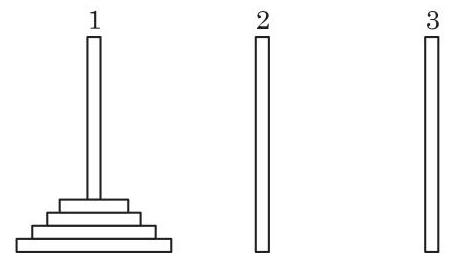
\includegraphics[max width=0.3\textwidth]{images/bo_d7fqvdc91nqc7381i9u0_181_572_1827_455_264_0.jpg}
\end{center}
\hspace*{3em} 

(第 1 题)

2. 如图, 将一个边长为 1 的正三角形的每条边三等分, 以中间一段为边向外作正三角形, 并擦去中间这一段, 如此继续下去得到的曲线称为科克雪花曲线. 将下面的图形依次记作 \({M}_{1}\text{ 、 }{M}_{2}\text{ 、 }{M}_{3}\text{ 、 }\cdots \text{ 、 }{M}_{n}\text{ 、 }\cdots\) .

\begin{center}
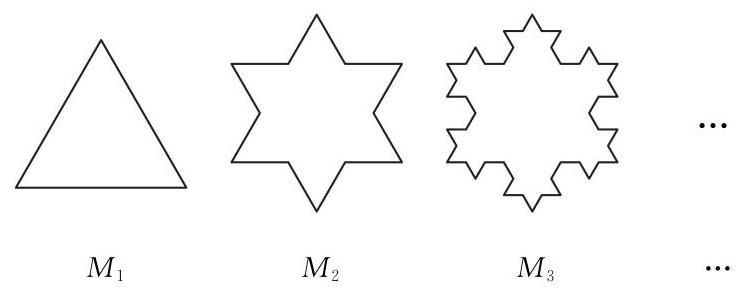
\includegraphics[max width=0.6\textwidth]{images/bo_d7fqvdc91nqc7381i9u0_182_474_401_741_294_0.jpg}
\end{center}
\hspace*{3em} 

(第 2 题)

(1)求 \({M}_{n}\) 的周长；

(2)求 \({M}_{n}\) 的面积；

(3)当 \(n \rightarrow   + \infty\) 时，科克雪花曲线所围成的图形是周长无限增大而面积却有极限的图形吗? 若是, 请求出其面积的极限; 若不是, 请说明理由.

\section*{后 记}

本套高中数学教材根据教育部颁布的《普通高中数学课程标准 (2017 年版 2020 年修订)》编写并经国家教材委员会专家委员会审核通过.

本教材是由设在复旦大学和华东师范大学的两个上海市数学教育教学研究基地(上海高校“立德树人”人文社会科学重点研究基地)联合主持编写的. 编写工作依据高中数学课程标准的具体要求，努力符合教育规律和高中学生的认知规律，结合上海城市发展定位和课程改革基础，并力求充分体现特色. 希望我们的这一努力能经得起实践和时间的检验, 对扎实推进数学的基础教育发挥积极的作用.

本册教材是选择性必修第一册，共为四章，各章编写人员分别为

曾国光(第 1 章)

虞涛、李英(第 2 章)

王华、施洪亮(第 3 章)

叶莎莎、许亚善(第 4 章)

上海市中小学(幼儿园)课程改革委员会专家工作委员会、上海市教育委员会教学研究室全程组织、指导和协调了教材编写工作. 在编写过程中，两个基地所在单位给予了大力支持，基地的全体同志积极参与相关的调研、讨论及评阅工作，发挥了重要的作用. 上海市不少中学也热情地参与了有关的调研及讨论工作. 有限公司不但是编辑出版单位, 而且自始至终全面介入了编写工作. 我们对所有这些单位和相关人员的参与、支持和鼓励表示衷心感谢.

限于编写者的水平, 也由于新编教材尚缺乏教学实践的检验, 不妥及疏漏之处在所难免，恳请广大师生及读者不吝赐教. 宝贵意见请通过邮箱 gaozhongshuxue@seph.com.cn 反馈, 不胜感激.

2020 年 7 月

SHUXUE 普通高中教科书数学

选择性必修

第 一 册

\begin{center}
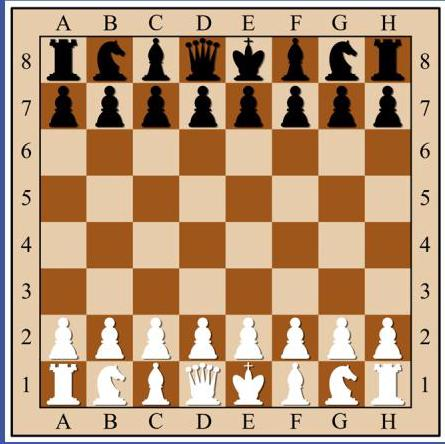
\includegraphics[max width=0.3\textwidth]{images/bo_d7fqvdc91nqc7381i9u0_184_602_1010_445_444_0.jpg}
\end{center}
\hspace*{3em} 

2024 蛰伏

精进

\section*{IATEX 实用功能简介}

整理错题、积累典型题、记录教学心得、整理解题笔记必备工具

编写试卷讲义、制作课件、出版校本教材的不二选择

数学老师的新一代生产力工具

向每一个选择长期主义的老师致敬

\section*{目录}

一、IATEX 是什么？软件的渊源、使用人群和 IATEX 生态 2

1.1 软件渊源 2

1.2 使用人群 2

1.3 IATEX 生态 2

二、软件功能简介 3

2.1 编辑数学公式高效、规范、稳定 3

2.2 编辑试卷、讲义、校本教材自动化程度高 4

2.3 画图高效、美观、方便修改与正文浑然一体 4

2.4 试题、讲义、校本教材效果展示 5

试卷 5

讲义 8

校本教材 9

知 幻灯片 10

2.5 数学作图方便、精准、美观与文档浑然一体 12

函数图 12

知立体图 12

统计图 12

知圆锥曲线图 13

知其他平面图 13

4 其它图形 14

知三视图 14

4 与文档浑然一体 16

三、课程简介与学习流程 17

附件二:公式效果 18

\section*{面向中学数学教师的 IATEX 培训课程手册}

\section*{一、 IATEX 是什么？软件的渊源、使用人群和 IATEX 生态}

\section*{1.1 软件渊源}

图灵奖得主高德纳教授在修订他的《计算机程序设计的艺术》(这本书的学界地位与《几何原本》、《相对论》、《量子力学》比肩而立) 第二卷时，因不满出版社的排版质量而自己设计了一个新的排版系统 TEX，这就是 LaTeX 的前身，经过兰伯特、美国数学学会以及其他的行业大咖不断维护更新, 形成了今天的 LATEX, 广泛应用于理工科文档编辑排版, 被誉为排版之王, 甚至很多杂志也要求用 IATEX 排版.

\section*{1.2 使用人群}

IATEX 以其在编辑数学公式方面无可比拟的优势而闻名于世, 目前在国外家喻户晓，在国内的使用者主要是大学理工科教授、研究所、科技企业、 出版社. 最早就是由中科院吴凌云等教授汉化软件并在国内推广的, 现在很多名校的理工科的研究生 (尤其是数学专业的研究生) 的毕业论文都必须使用IATEX 完成。

\section*{1.3 IATEX 生态}

IATEX 已经作为行业标准, 广泛应用于和公式编辑相关的大多数场景, 越来越多的公司提供相关服务，比如 mathpix、腾讯云、有道云都可以将图片版的数学公式转化为 \(\mathrm{I}\) ATEX,可以大大提高公式的输入效率. 越来越多的出版社包括科学出版社、中科大出版社、浙江大学出版社、清华大学出版社支持 IATEX 书稿出版.

随着中学教师的学历的不断提升，电脑的普及，信息化能力的提升，很多教师都萌生了整理自己的教学成果，教学资料的想法，以前苦于没有良好的工具, 自从 LATEX 被引进中学老师圈, 越来越多的中学老师使用 LATEX 编辑整理教案、讲义、试卷、画图、校本教材，使用 IATEX 在中学已经蔚然成风.

\section*{二、软件功能简介}

\section*{2.1 编辑数学公式高效、规范、稳定}

IATEX 输入数学公式全部通过键盘的, 而不需要像公式编辑器那样通过鼠标点击来回切换插入公式，减少麻烦，另外 LATEX 的符号更加全面，老师们不会因为找不到符号而苦恼.

除了编辑效率高, 还有规范、稳定的优势. LATEX 编辑的公式与文本格式统一, 大小字号也可以统一调整, 也可以任意复制粘贴, 在任意电脑上播放, 永不变形、不错位、不乱码, 受到老师们的一致喜爱. 以下为效果:

\[
f\left( x\right)  = \left\{  \begin{array}{ll} {x}^{2} - {2x} + 3, & x \leq  1, \\  x - 2, & x > 1. \end{array}\right. \;\left\{  \begin{array}{l} \widehat{b} = \frac{\mathop{\sum }\limits_{{i = 1}}^{n}\left( {{x}_{i} - \bar{x}}\right) \left( {{y}_{i} - \bar{y}}\right) }{\mathop{\sum }\limits_{{i = 1}}^{n}{\left( {x}_{i} - \bar{x}\right) }^{2}} = \frac{\mathop{\sum }\limits_{{i = 1}}^{n}{x}_{i}{y}_{i} - n\bar{x}\bar{y}}{\mathop{\sum }\limits_{{i = 1}}^{n}{x}_{i}^{2} - n{\bar{x}}^{2}} \\  \widehat{a} = \bar{y} - \widehat{b}\bar{x} \end{array}\right.
\]

\[
\mathop{\sum }\limits_{{i = 1}}^{n}\left( {{x}_{i} - \bar{x}}\right) \left( {{y}_{i} - \bar{y}}\right)
\]

\[
= \left( {{x}_{1} - \bar{x}}\right) \left( {{y}_{1} - \bar{y}}\right)  + \left( {{x}_{2} - \bar{x}}\right) \left( {{y}_{2} - \bar{y}}\right)  + \cdots \left( {{x}_{n} - \bar{x}}\right) \left( {{y}_{n} - \bar{y}}\right)
\]

\[
= \left( {{x}_{1}{y}_{1} - {x}_{1}\bar{y} - \bar{x}{y}_{1} + \bar{x}\bar{y}}\right)  + \left( {{x}_{2}{y}_{2} - {x}_{2}\bar{y} - \bar{x}{y}_{2} + \bar{x}\bar{y} + \cdots  + \left( {{x}_{n}{y}_{n} - {x}_{n}\bar{y} - \bar{x}{y}_{n} + \bar{x}\bar{y}}\right) }\right.
\]

\[
= \left( {{x}_{1}{y}_{1} + {x}_{2}{y}_{2} + \cdots  + {x}_{n}{y}_{n}}\right)  - \left( {{x}_{1} + {x}_{2} + \cdots  + {x}_{n}}\right) \bar{y} - \bar{x}\left( {{y}_{1} + {y}_{2} + \cdots  + {y}_{n}}\right)  + n\bar{x}\bar{y}
\]

\[
= \mathop{\sum }\limits_{{i = 1}}^{n}{x}_{i}{y}_{i} - \left( {\mathop{\sum }\limits_{{i = 1}}^{n}{x}_{i}}\right) \bar{y} - \bar{x}\left( {\mathop{\sum }\limits_{{i = 1}}^{n}{y}_{i}}\right)  + n\bar{x}\bar{y}
\]

\[
= \mathop{\sum }\limits_{{i = 1}}^{n}{x}_{i}{y}_{i} - n\bar{x} \cdot  \bar{y} - \bar{x} \cdot  n\bar{y} + n\bar{x}\bar{y}
\]

\[
= \mathop{\sum }\limits_{{i = 1}}^{n}{x}_{i}{y}_{i} - n\bar{x}\bar{y}
\]

很多老师在准备公开课时, 由于公式编辑器的效率低甚至符号不全, 大多选择拼凑、修改一些课件，而这些课件的公式格式混乱、不规范，修改的时间比重新输入都要长,让老师们感到精疲力尽. LATEX 的编辑效率高、规范、稳定, 公式直接编辑就行了, 让老师把主要精力放到作课的思路上, 节约老师大量时间和心理成本.

\section*{2.2 编辑试卷、讲义、校本教材自动化程度高}

IATEX 自动化程度高最重要的体现方面是可以一键控制是否显示试题的答案、分析、详细解析, 从而得到学生版和教师版, 也可以单独得到答案, 这个过程不需要逐一的剪切、粘贴答案. 另外也可以实现:

1. 试题的来源、难度等试题标识能够一键控制是否显示;

2. 能够一键设置 A4 纸、A3 纸，单栏、双栏、多栏，无需过多调整；

3. 题号自动生成、对齐，调换顺序不用手动编号，不用担心答案不匹配；

4. 试题后的距离, 可一键控制是否显示, 可根据需要给学生留作答空间;

5. 选择题的选项可以自动排版, 会根据选项的长短自动确定一行排四个、 两个或一个选项, 选择题括号生成、自动右对齐;

6. 解答题的序号可以一键全部设置为罗马数字或阿拉伯数字.

这些自动化的设计极大地提高了教师整理试题、编写文档的效率，方便老师整理自己的讲义, 给学生更有针对性的出题, 布置作业. 还可以给讲义设置很多漂亮的文档结构, 也可以根据实际需要定制各种各样的功能.

\section*{2.3 画图高效、美观、方便修改与正文浑然一体}

数学画图是中学老师们遇到的另一个难题, 虽然也有几何画板、GeoGe-bra 等诸多软件可以画图, 但是也会存在一些问题, 比如:

1. 很多图画得慢, 不精确, 甚至画不出来. 如: 立体图、程序框图等;

2. 在图中输入数学公式比较麻烦, 图中文字的字体、大小也不容易统一;

3. 清晰度不高. 将其他软件制作的图插入文档，清晰的度会降低.

4. 细节调整比较麻烦, 后期修改不方便. 比如: 调整坐标轴的箭头, 坐标的位置等比较麻烦, 如果后期修改之前图中的错误, 几乎需要重做.

IATEX 画图可以完美解决这些问题, 不仅仅前期画图方便, 字体字号可以统一调整, 图中可以插入任意公式, 自由编辑. 在可修改性和复用性方面更是无可比拟. 比如题干中画好的图, 在解析中仍然可以在画好的图上进行编辑.

接下来我们来看具体效果.

\section*{2.4 试题、讲义、校本教材效果展示}

\section*{试卷}

按秘密事项管理 \ding{72} 启用前

\section*{2024 全国新课标 I 卷}

\section*{一、选择题: 本大题共 8 小题, 每小题 5 分, 共 40 分. 在每小题给出的四个选项中, 只有 一项是符合题目要求的.}

1. 已知集合 \(A = \left\{  {x \mid   - 5 < {x}^{3} < 5}\right\}  ,B = \{  - 3, - 1,0,2,3\}\) ,则 \(A \cap  B =\) ( )

A. \(\{  - 1,0\}\) B. \(\{ 2,3\}\) C. \(\{  - 3, - 1,0\}\) D. \(\{  - 1,0,2\}\)

2. 若 \(\frac{z}{z - 1} = 1 + \mathrm{i}\) ,则 \(z =\) ( )

A. \(- 1 - \mathrm{i}\) B. \(- 1 + \mathrm{i}\) C. \(1 - \mathrm{i}\) D. \(1 + \mathrm{i}\)

3. 已知向量 \(\mathbf{a} = \left( {0,1}\right) ,\mathbf{b} = \left( {2,x}\right)\) ,若 \(\mathbf{b} \bot  \left( {\mathbf{b} - 4\mathbf{a}}\right)\) ,则 \(x =\) ( )

A. -2 B. -1 C. 1 D. 2

4. 已知 \(\cos \left( {\alpha  + \beta }\right)  = m,\tan \alpha \tan \beta  = 2\) ,则 \(\cos \left( {\alpha  - \beta }\right)  =\) ( )

A. \(- {3m}\) B. \(- \frac{m}{3}\) C. \(\frac{m}{3}\) D. \({3m}\)

5. 已知圆柱和圆锥的底面半径相等，侧面积相等，且它们的高均为 \(\sqrt{3}\) ，则圆锥的体积为 ( )

A. \(2\sqrt{3}\pi\) B. \(3\sqrt{3}\pi\) C. \(6\sqrt{3}\pi\) D. \(9\sqrt{3}\pi\)

6. 已知函数 \(f\left( x\right)  = \left\{  \begin{matrix}  - {x}^{2} - {2ax} - a, & x < 0 \\  {\mathrm{e}}^{x} + \ln \left( {x + 1}\right) , & x \geq  0 \end{matrix}\right.\) 在 \(\mathbf{R}\) 上单调递增,则 \(a\) 的取值范围是 ( )

A. \(( - \infty ,0\rbrack\) B. \(\left\lbrack  {-1,0}\right\rbrack\) C. \(\left\lbrack  {-1,1}\right\rbrack\) D. \(\lbrack 0, + \infty )\)

7. 当 \(x \in  \left\lbrack  {0,{2\pi }}\right\rbrack\) 时,曲线 \(y = \sin x\) 与 \(y = 2\sin \left( {{3x} - \frac{\pi }{6}}\right)\) 的交点个数为 ( )

A. 3 B. 4 C. 6 D. 8

8. 已知函数为 \(f\left( x\right)\) 的定义域为 \(\mathbf{R},f\left( x\right)  > f\left( {x - 1}\right)  + f\left( {x - 2}\right)\) ,且当 \(x < 3\) 时, \(f\left( x\right)  = x\) , 则下列结论中一定正确的是 ( )

A. \(f\left( {10}\right)  > {100}\) B. \(f\left( {20}\right)  > {1000}\) C. \(f\left( {10}\right)  < {1000}\) D. \(f\left( {20}\right)  < {10000}\)

\section*{二、选择题: 本题共 3 小题, 每小题 6 分, 共 18 分. 在每小题给出的选项中, 有多项符合 题目要求. 全部选对的得 6 分, 部分选对的得部分分, 有选错的得 0 分.}

9. 多选题:随着”一带一路”国际合作的深入，某茶叶种植区多措并举推动茶叶出口. 为了解推动出口后的亩收入 (单位: 万元) 情况, 从该种植区抽取样本, 得到推动出口后亩收入的样本均值 \(\bar{x} = {2.1}\) ,样本方差 \({s}^{2} = {0.01}\) ,已知该种植区以往的亩收入 \(X\) 服从正态分布 \(N\left( {{1.8},{0.1}^{2}}\right)\) . 假设推动出口后的亩收入 \(Y\) 服从正态分布 \(N\left( {\bar{x},{s}^{2}}\right)\) ,则 (若随机变量 \(Z\) 服从正态分布 \(N\left( {\mu ,{\sigma }^{2}}\right)\) ,则 \(P\left( {Z < \mu  + \sigma }\right)  \approx  {0.8413}\) ) ( )

A. \(P\left( {X > 2}\right)  > {0.2}\) B. \(P\left( {X > 2}\right)  < {0.5}\) C. \(P\left( {Y > 2}\right)  > {0.5}\) D. \(P\left( {Y > 2}\right)  < {0.8}\) 10. 多选题,设函数 \(f\left( x\right)  = {\left( x - 1\right) }^{2}\left( {x - 4}\right)\) ,则 ( )

A. \(x = 3\) 是 \(f\left( x\right)\) 的极小值点 B. 当 \(0 < x < 1\) 时, \(f\left( x\right)  < f\left( {x}^{2}\right)\)

C. 当 \(1 < x < 2\) 时, \(- 4 < f\left( {{2x} - 1}\right)  < 0\) D. 当 \(- 1 < x < 0\) 时, \(f\left( {2 - x}\right)  > f\left( x\right)\)

\begin{center}
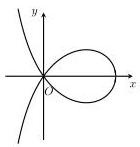
\includegraphics[max width=0.2\textwidth]{images/bo_d7fqvdc91nqc7381i9u0_190_1323_722_140_147_0.jpg}
\end{center}
\hspace*{3em} 

11. (多选题) 设计一条美丽的丝带,其造型 \(\smallsetminus   \text{ ○ }\) 可以看作图中的曲线 \(C\) 的一部分,已知 \(C\) 过坐标原点 \(O\) ,且 \(C\) 上的点满足横坐标大于 -2,到点 \(F\left( {2,0}\right)\) 的距离与到定直线 \(x = a\left( {a < 0}\right)\) 的距离之积为 4 , 则 ( )

A. \(a =  - 2\)

B. 点 \(\left( {2\sqrt{2},0}\right)\) 在 \(C\) 上

C. \(C\) 在第一象限的点的纵坐标的最大值为 1

D. 当点 \(\left( {{x}_{0},{y}_{0}}\right)\) 在 \(C\) 上时, \({y}_{0} \leq  \frac{4}{{x}_{0} + 2}\)

\section*{三、填空题:本大题共 3 小题，每小题 5 分，共 15 分.}

12. 设双曲线 \(C : \frac{{x}^{2}}{{a}^{2}} - \frac{{y}^{2}}{{b}^{2}} = 1\left( {a > 0,b > 0}\right)\) 的左右焦点分别为 \({F}_{1},{F}_{2}\) ,过 \({F}_{2}\) 作平行于 \(y\) 轴的直线交 \(C\) 于 \(A,B\) 两点,若 \(\left| {{F}_{1}A}\right|  = {13},\left| {AB}\right|  = {10}\) ,则 \(C\) 的离心率为 .

13. 若曲线 \(y = {\mathrm{e}}^{x} + x\) 在点 \(\left( {0,1}\right)\) 处的切线也是曲线 \(y = \ln \left( {x + 1}\right)  + a\) 的切线,则 \(a =\)

2024 全国新课标 I 卷 第 1 页 共 2 页

14. 甲、乙两人各有四张卡片，每张卡片上标有一个数字，甲的卡片上分别标有数字 1,3,5,7,乙的卡片上分别标有数字2,4,6,8. 两人进行四轮比赛,在每轮比赛中,两人各自从自己持有的卡片中随机选一张，并比较所选卡片上数字的大小，数字大的人得 1 分, 数字小的人得 0 分, 然后各自弃置此轮所选的卡片 (弃置的卡片在此后的轮次中不能使用). 则四轮比赛比赛后, 甲的总得分不小于 2 的概率为

\section*{四、解答题:本大题共 5 小题, 共 77 分. 解答应写出必要的文字说明、证明过程或演算 步骤.}

15. 记 \(\bigtriangleup {ABC}\) 的内角 \(A,B,C\) 的对边分别为 \(a,b,c\) ,已知 \(\sin C = \sqrt{2}\cos B,{a}^{2} + {b}^{2} - {c}^{2} = \; \sqrt{2}{ab}\) .

( 1 ) 求 \(B\) ;

(2) 若 \(\bigtriangleup {ABC}\) 的面积为 \(3 + \sqrt{3}\) ,求 \(c\) .

16. 已知 \(A\left( {0,3}\right)\) 和 \(P\left( {3,\frac{3}{2}}\right)\) 为椭圆 \(C : \frac{{x}^{2}}{{a}^{2}} + \frac{{y}^{2}}{{b}^{2}} = 1\left( {a > b > 0}\right)\) 上两点.

( 1 ) 求 \(C\) 的离心率;

( 2 ) 若过 \(P\) 的直线 \(l\) 交 \(C\) 于另一点 \(B\) ,且 \(\bigtriangleup {ABP}\) 的面积为 9,求 \(l\) 的方程.

17. 如图,四棱锥 \(P - {ABCD}\) 中, \({PA} \bot\) 底面 \({ABCD},{PA} = {AC} = 2,{BC} = 1,{AB} = \sqrt{3}\) .

( 1 ) 若 \({AD} \bot  {PB}\) ,证明: \({AD}//\) 平面 \({PBC}\) ;

( 2 ) 若 \({AD} \bot  {DC}\) ,且二面角 \(A - {CP} - D\) 的正弦值为 \(\frac{\sqrt{42}}{7}\) ,求 \({AD}\) .

\begin{center}
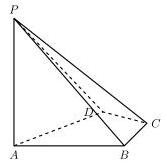
\includegraphics[max width=0.2\textwidth]{images/bo_d7fqvdc91nqc7381i9u0_190_687_1911_167_163_0.jpg}
\end{center}
\hspace*{3em} 

18. 已知函数 \(f\left( x\right)  = \ln \frac{x}{2 - x} + {ax} + b{\left( x - 1\right) }^{3}\)

( 1 ) 若 \(b = 0\) ,且 \({f}^{\prime }\left( x\right)  \geq  0\) ,求 \(a\) 的最小值;

( 2 ) 证明: 曲线 \(y = f\left( x\right)\) 是中心对称图形;

( 3 ) 若 \(f\left( x\right)  >  - 2\) ,当且仅当 \(1 < x < 2\) ,求 \(b\) 的取值范围.

19. 设 \(m\) 为正整数,数列 \({a}_{1},{a}_{2},\cdots ,{a}_{{4m} + 2}\) 是公差不为 0 的等差数列,若从中删去两项 \({a}_{i}\) 和 \({a}_{j}\left( {i < j}\right)\) 后剩余的 \({4m}\) 项可被平均分为 \(m\) 组,且每组的 4 个数都能构成等差数列,则称数列 \({a}_{1},{a}_{2},\cdots ,{a}_{{4m} + 2}\) 是 \(\left( {i,j}\right)\) - 可分数列.

(1)写出所有的 \(\left( {i,j}\right) ,1 \leq  i < j \leq  6\) ,使数列 \({a}_{1},{a}_{2},\cdots ,{a}_{6}\left( {i,j}\right)\) - 可分数列;

( 2 ) 当 \(m \geq  3\) 时,证明: 数列 \({a}_{1},{a}_{2},\cdots ,{a}_{{4m} + 2}\) 是 \(\left( {2,{13}}\right)  -\) 可分数列;

( 3 ) 从 \(1,2,\cdots ,{4m} + 2\) 中一次任取两个数 \(i\) 和 \(j\left( {i < j}\right)\) ,记数列 \({a}_{1},{a}_{2},\cdots ,{a}_{{4m} + 2}\) 是 \(\left( {i,j}\right)\) - 可分数列的概率为 \({P}_{m}\) ,证明 \({P}_{m} > \frac{1}{8}\) .

按秘密事项管理 \ding{72} 启用前

\section*{2024 全国新课标 I 卷}

一、选择题: 本大题共 8 小题, 每小题 5 分, 共 40 分. 在每小题给出的四个选项中, 只有一项是符合题目要求的.

1. 已知集合 \(A = \left\{  {x \mid   - 5 < {x}^{3} < 5}\right\}  ,B = \{  - 3, - 1,0,2,3\}\) ,则 \(A \cap  B =\)

A. \(\{  - 1,0\}\) B. \(\{ 2,3\}\) C. \(\{  - 3, - 1,0\}\) D. \(\{  - 1,0,2\}\)

2. 若 \(\frac{z}{z - 1} = 1 + \mathrm{i}\) ,则 \(z =\) ( )

A. \(- 1 - \mathrm{i}\) B. \(- 1 + \mathrm{i}\) C. \(1 - \mathrm{i}\) D. \(1 + \mathrm{i}\)

3. 已知向量 \(\mathbf{a} = \left( {0,1}\right) ,\mathbf{b} = \left( {2,x}\right)\) ,若 \(\mathbf{b} \bot  \left( {\mathbf{b} - 4\mathbf{a}}\right)\) ,则 \(x =\) ( )

A. -2 B. -1 C. 1 D. 2

4. 已知 \(\cos \left( {\alpha  + \beta }\right)  = m,\tan \alpha \tan \beta  = 2\) ,则 \(\cos \left( {\alpha  - \beta }\right)  =\) ( )

A. \(- {3m}\) B. \(- \frac{m}{3}\) C. \(\frac{m}{3}\) D. \({3m}\)

5. 已知圆柱和圆锥的底面半径相等，侧面积相等，且它们的高均为 \(\sqrt{3}\) ，则圆锥的体积为 ( )

A. \(2\sqrt{3}\pi\) B. \(3\sqrt{3}\pi\) C. \(6\sqrt{3}\pi\) D. \(9\sqrt{3}\pi\)

6. 已知函数 \(f\left( x\right)  = \left\{  \begin{array}{ll}  - {x}^{2} - {2ax} - a, & x < 0 \\  {\mathrm{e}}^{x} + \ln \left( {x + 1}\right) , & x \geq  0 \end{array}\right.\) 在 \(\mathbf{R}\) 上单调递增,则 \(a\) 的取值范围是 ( A. \(( - \infty ,0\rbrack\) B. \(\left\lbrack  {-1,0}\right\rbrack\) C. \(\left\lbrack  {-1,1}\right\rbrack\) D. \(\lbrack 0, + \infty )\)

7. 当 \(x \in  \left\lbrack  {0,{2\pi }}\right\rbrack\) 时,曲线 \(y = \sin x\) 与 \(y = 2\sin \left( {{3x} - \frac{\pi }{6}}\right)\) 的交点个数为

A. 3 B. 4 C. 6 D. 8

关注【觅宁参考】即可联系作者，获取无水印有答案版本，也可以学公式编辑与排版

关注微信公众号:宽宁参考

三、填空题:本大题共 3 小题，每小题 5 分，共 15 分.

12. 设双曲线 \(C : \frac{{x}^{2}}{{a}^{2}} - \frac{{y}^{2}}{{b}^{2}} = 1\left( {a > 0,b > 0}\right)\) 的左右焦点分别为 \({F}_{1},{F}_{2}\) ,过 \({F}_{2}\) 作平行于 \(y\) 轴的直线交 \(C\) 于 \(A,B\) 两点,若 \(\left| {{F}_{1}A}\right|  = {13},\left| {AB}\right|  = {10}\) ,则 \(C\) 的离心率为

13. 若曲线 \(y = {\mathrm{e}}^{x} + x\) 在点 \(\left( {0,1}\right)\) 处的切线也是曲线 \(y = \ln \left( {x + 1}\right)  + a\) 的切线,则 \(a =\) \_\_\_\_\_.

14. 甲、乙两人各有四张卡片，每张卡片上标有一个数字，甲的卡片上分别标有数字 1,3,5,7,乙的卡片上分别标有数字2,4,6,8. 两人进行四轮比赛,在每轮比赛中,两人各自从自己持有的卡片中随机选一张, 并比较所选卡片上数字的大小, 数字大的人得 1 分, 数字小的人得 0 分, 然后各自弃置此轮所选的卡片 (弃置的卡片在此后的轮次中不能使用). 则四轮比赛比赛后, 甲的总得分不小于 2 的概率为 .

四、解答题:本大题共 5 小题, 共 77 分. 解答应写出必要的文字说明、证明过程或演算步骤.

15. 记 \(\bigtriangleup {ABC}\) 的内角 \(A,B,C\) 的对边分别为 \(a,b,c\) ,已知 \(\sin C = \sqrt{2}\cos B,{a}^{2} + {b}^{2} - {c}^{2} = \; \sqrt{2}{ab}\) .

( 1 ) 求 \(B\) ;

(2 ) 若 \(\bigtriangleup {ABC}\) 的面积为 \(3 + \sqrt{3}\) ,求 \(c\) .

16. 已知 \(A\left( {0,3}\right)\) 和 \(P\left( {3,\frac{3}{2}}\right)\) 为椭圆 \(C : \frac{{x}^{2}}{{a}^{2}} + \frac{{y}^{2}}{{b}^{2}} = 1\left( {a > b > 0}\right)\) 上两点.

(1)求 \(C\) 的离心率；

(2)若过 \(P\) 的直线 \(l\) 交 \(C\) 于另一点 \(B\) ,且 \(\bigtriangleup {ABP}\) 的面积为 9,求 \(l\) 的方程.

8. 已知函数为 \(f\left( x\right)\) 的定义域为 \(\mathbf{R},f\left( x\right)  > f\left( {x - 1}\right)  + f\left( {x - 2}\right)\) ,且当 \(x < 3\) 时, \(f\left( x\right)  = x\) , 则下列结论中一定正确的是 (   )

A. \(f\left( {10}\right)  > {100}\) B. \(f\left( {20}\right)  > {1000}\) C. \(f\left( {10}\right)  < {1000}\) D. \(f\left( {20}\right)  < {10000}\)

二、选择题: 本题共 3 小题, 每小题 6 分, 共 18 分. 在每小题给出的选项中, 有多项符合题目要求. 全部选对的得 6 分, 部分选对的得部分分, 有选错的得 0 分.

9. 随着”一带一路”国际合作的深入，某茶叶种植区多措并举推动茶叶出口. 为了解推动出口后的亩收入 (单位: 万元) 情况, 从该种植区抽取样本, 得到推动出口后亩收入的样本均值 \(\bar{x} = {2.1}\) ,样本方差 \({s}^{2} = {0.01}\) ,已知该种植区以往的亩收入 \(X\) 服从正态分布 \(N\left( {{1.8},{0.1}^{2}}\right)\) . 假设推动出口后的亩收入 \(Y\) 服从正态分布 \(N\left( {\bar{x},{s}^{2}}\right)\) ,则 (若随机变量 \(Z\) 服从正态分布 \(N\left( {\mu ,{\sigma }^{2}}\right)\) ,则 \(P\left( {Z < \mu  + \sigma }\right)  \approx  {0.8413})\) ( )

A. \(P\left( {X > 2}\right)  > {0.2}\) B. \(P\left( {X > 2}\right)  < {0.5}\) C. \(P\left( {Y > 2}\right)  > {0.5}\) D. \(P\left( {Y > 2}\right)  < {0.8}\)

10. 设函数 \(f\left( x\right)  = {\left( x - 1\right) }^{2}\left( {x - 4}\right)\) ,则 ( )

A. \(x = 3\) 是 \(f\left( x\right)\) 的极小值点 B. 当 \(0 < x < 1\) 时, \(f\left( x\right)  < f\left( {x}^{2}\right)\)

C. 当 \(1 < x < 2\) 时, \(- 4 < f\left( {{2x} - 1}\right)  < 0\) D. 当 \(- 1 < x < 0\) 时, \(f\left( {2 - x}\right)  > f\left( x\right)\)

\begin{center}
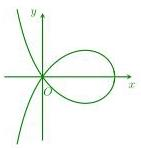
\includegraphics[max width=0.2\textwidth]{images/bo_d7fqvdc91nqc7381i9u0_191_1325_737_141_148_0.jpg}
\end{center}
\hspace*{3em} 

11. 设计一条美丽的丝带,其造型 \(\smallsetminus   \text{ ○ }\) 可以看作图中的曲线 \(C\) 的一部分,已知 \(C\) 过坐标原点 \(O\) ,且 \(C\) 上的点满足横坐标大于 -2,到点 \(F\left( {2,0}\right)\) 的距离与到定直线 \(x = a\left( {a < 0}\right)\) 的距离之积为 4 , 则 ( )

A. \(a =  - 2\)

B. 点 \(\left( {2\sqrt{2},0}\right)\) 在 \(C\) 上

C. \(C\) 在第一象限的点的纵坐标的最大值为 1

D. 当点 \(\left( {{x}_{0},{y}_{0}}\right)\) 在 \(C\) 上时, \({y}_{0} \leq  \frac{4}{{x}_{0} + 2}\)

17. 如图,四棱锥 \(P - {ABCD}\) 中, \({PA} \bot\) 底面 \({ABCD},{PA} = {AC} = 2,{BC} = 1,{AB} = \sqrt{3}\) . (1) 若 \({AD} \bot  {PB}\) ,证明: \({AD}//\) 平面 \({PBC}\) ;

( 2 ) 若 \({AD} \bot  {DC}\) ,且二面角 \(A - {CP} - D\) 的正弦值为 \(\frac{\sqrt{42}}{7}\) ,求 \({AD}\) .

\begin{center}
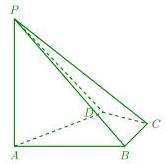
\includegraphics[max width=0.2\textwidth]{images/bo_d7fqvdc91nqc7381i9u0_191_1314_1236_166_164_0.jpg}
\end{center}
\hspace*{3em} 

18. 已知函数 \(f\left( x\right)  = \ln \frac{x}{2 - x} + {ax} + b{\left( x - 1\right) }^{3}\)

( 1 ) 若 \(b = 0\) ,且 \({f}^{\prime }\left( x\right)  \geq  0\) ,求 \(a\) 的最小值;

( 2 ) 证明: 曲线 \(y = f\left( x\right)\) 是中心对称图形;

( 3 ) 若 \(f\left( x\right)  >  - 2\) ,当且仅当 \(1 < x < 2\) ,求 \(b\) 的取值范围.

19. 设 \(m\) 为正整数,数列 \({a}_{1},{a}_{2},\cdots ,{a}_{{4m} + 2}\) 是公差不为 0 的等差数列,若从中删去两项 \({a}_{i}\) 和 \({a}_{j}\left( {i < j}\right)\) 后剩余的 \({4m}\) 项可被平均分为 \(m\) 组,且每组的 4 个数都能构成等差数列,则称数列 \({a}_{1},{a}_{2},\cdots ,{a}_{{4m} + 2}\) 是 \(\left( {i,j}\right)\) - 可分数列.

( 1 ) 写出所有的 \(\left( {i,j}\right) ,1 \leq  i < j \leq  6\) ,使数列 \({a}_{1},{a}_{2},\cdots ,{a}_{6}\left( {i,j}\right)\) - 可分数列;

( 2 ) 当 \(m \geq  3\) 时,证明: 数列 \({a}_{1},{a}_{2},\cdots ,{a}_{{4m} + 2}\) 是 \(\left( {2,{13}}\right)\) - 可分数列;

( 3 ) 从 \(1,2,\cdots ,{4m} + 2\) 中一次任取两个数 \(i\) 和 \(j\left( {i < j}\right)\) ,记数列 \({a}_{1},{a}_{2},\cdots ,{a}_{{4m} + 2}\) 是 \(\left( {i,j}\right)\) - 可分数列的概率为 \({P}_{m}\) ,证明 \({P}_{m} > \frac{1}{8}\) .

\section*{试题 + 答案版本和纯答案版本}

按秘密事项管理 \ding{72} 启用前 【解答】

2022 年普通高等学生招生全国统一考试 (模拟卷) 4.

( )

数 学 A. B. C. D.

【考试声明】

【分析】

【简要答案】

1. 认真考试，不要作弊，可以百度答案，但是百度不了人生; 【解答】

5.

2. 把答案写到答题卡上;

3. 参考公式:我就不写了；

( )

一、选择题:本大题共 12 小题，每小题 5 分，共 60 分。在每小题给出的四个选项中，只有一项是符合题目要求的。 A. B. C. D.

【分析】

1. 【简要答案】

( ) 【解答】

A. B. C. 6.

【分析】 ( )

【简要答案】 A. B. C. D.

【解答】 【分析】

2. 【简要答案】

( ) 【解答】

A. B. C. 7.

【分析】 ( )

【简要答案】 A. B. C. D.

【解答】 【分析】

3. 【简要答案】

【解答】

A. B. C. D. 8.

【分析】

【简要答案】

按秘密事项管理 \ding{72} 启用前 7.【分析】

2022 年普通高等学生招生全国统一考试(模拟卷) 【简要答案】

【解答】

数 学 8.【分析】

【考试声明】

【简要答案】

【解答】

1. 认真考试，不要作弊，可以百度答案，但是百度不了人生;

9.【分析】

2. 把答案写到答题卡上;

【简要答案】

3. 参考公式:我就不写了；

【解答】

一、选择题:本大题共 12 小题，每小题 5 分，共 60 分。在每小题给出的四个选项中，只有一项是符合题目要求的。 10.【分析】

【简要答案】

1.【分析】 【解答】

【简要答案】 11.【分析】

【解答】 【简要答案】

2.【分析】 【解答】

【简要答案】 12.【分析】

【解答】 【简要答案】

3.【分析】 【解答】

【简要答案】 二、填空题:本大题共 4 小题，每小题 5 分，共 20 分。把答案填写在题中的横线上。

【解答】 13.【分析】

4.【分析】 【简要答案】

【简要答案】 【解答】

14.【分析】

5.【分析】 【简要答案】

【简要答案】 【解答】

【解答】 15.【分析】

6.【分析】 【简要答案】

【简要答案】 【解答】

【解答】 16.【分析】

第 1 页 共 2 页

讲义

\section*{导数 函数单调性的讨论}

\section*{觅宁参考出品}

\section*{【主要内容】}

口典例精炼 3. 含参二次函数单调性的讨论

1. 含参一次函数单调性的讨论 4. 类含参二次函数单调性的讨论

2. 类含参一次函数单调性的讨论 5. 超越函数的零点问题

\section*{【核心逻辑】}

讨论参数的不同，得到导函数的单调性和导函数零点判断导函数在相应区间的正负，进而判断原函数的单调性.

\section*{【问题方法】}

一、求不含参函数的单调区间

1. 求函数定义域 易漏

2. 求出原函数的导函数,解出 \({f}^{\prime }\left( x\right)  = 0\) 的根 \({x}_{1},{x}_{2},\cdots\) ;

3. 用 \({x}_{1},{x}_{2},\cdots\) 将定义域划分为若干单调区间,分别计算每个区间上导函数的正负值;

4. 画出原函数的草图检验, 然后总结作答.

注意 若相邻两个单调区间的单调性一致, 则可视为一个单调区间.

二、含参一次函数单调性的讨论

1. 讨论最高次项是否为 0 ，正负情况 易漏

2. 求解导函数的根;

3. 定义域划分为若干单调区间, 分别讨论每个区间上导函数的正负值.

三、含参二次函数单调性的讨论

核心逻辑 就是三讨论: 讨论开口方向、讨论两根大小、讨论根的数量.

讨论开口方向观察二次项系数是否含参，如果含参，注意讨论开口方向(包括是否为 0 \()\) . 易漏

讨论两根大小观察能否分解因式, 能分解因式的, 注意比较两根大小, 以及两根

是否相等;

讨论根的数量如果不能分解因式, 计算判别式, 根据情况讨论;

方法步骤

(1)求函数定义域，求出原函数的导函数

(2)讨论最高次项是否为 0，正负情况；

(a) \(\left\{  \begin{array}{l} \text{ 可以分解因式 } \Rightarrow  \text{ 解得 }{x}_{1},{x}_{2}\text{ (注意讨论 }{x}_{1} = {x}_{2}\text{ ) } \\  \text{ 不能分解 } \Rightarrow  \left\{  \begin{array}{l} \Delta  \leq  0 \\  \Delta  > 0 \end{array}\right.  \end{array}\right.\)

(3)讨论 \({x}_{1}\) 和 \({x}_{2}\) 的大小，能分解因式的，注意讨论 \({x}_{1} = {x}_{2}\) .

(4) \({x}_{1}\) ， \({x}_{2}\) 将定义域划分为若干单调区间，分别讨论每个区间上导函数的正负值. 四、超越函数的零点问题

超越函数的零点, 关键在于零点的求解, 而一般超越函数的零点是不可解, 那么我们的方法有三:

1. 从题意中获取.

2. 试根. 一般是让对数式、指数式等于 0 或 1 等特殊值.

3. 零点本身不可解. 一般求出零点满足的关系式与取值范围，用 \({x}_{0}\) 表示这个零点, 这就是通常所说的隐零点.

\section*{【知识清单】}

在某个区间 \(\left( {a,b}\right)\) 内,

如果 \({f}^{\prime }\left( x\right)  > 0\) ,那么函数 \(y = f\left( x\right)\) 在这个区间内单调递增;

如果 \({f}^{\prime }\left( x\right)  < 0\) ,那么函数 \(y = f\left( x\right)\) 在这个区间内单调递减.

***典例精练***

\section*{一、对回归方程的理解}

1. (2012 湖南理 4(4/8) \ding{72}  \ding{73}  \ding{73}  \ding{73}  \ding{73}  \ding{73} )

设某大学的女生体重 \(y\) (单位: \(\mathrm{{kg}}\) ) 与身高 \(x\) (单位: \(\mathrm{{cm}}\) ) 具有线性相关关系,根据一组样本数据 \(\left( {{x}_{i},{y}_{i}}\right) \left( {i = 1,2,\cdots ,n}\right)\) ,用最小二乘法建立的回归方程为 \(y = \; {0.85x} - {85.71}\) ,则下列结论中不正确的是

A. \(y\) 与 \(x\) 具有正的线性相关关系

B. 回归直线过样本点的中心 \(\left( {\bar{x},\bar{y}}\right)\)

C. 若该大学某女生身高增加 \(1\mathrm{\;{cm}}\) ，则其体重约增加 \({0.85}\mathrm{\;{kg}}\)

D. 若该大学某女生身高为 170 cm，则可断定其体重必为 58.79 kg

2. (2012 全国 I 文 \(3\left( {3/{12}}\right)  \star   \star   \star   \star   \star   \star\) 交

在一组样本数据 \(\left( {{x}_{i},{y}_{1}}\right) ,\left( {{x}_{2},{y}_{2}}\right) ,\cdots ,\left( {{x}_{n},{y}_{n}}\right) \left( {n \geq  2,{x}_{1},{x}_{2},\cdots ,{x}_{n}}\right.\) 不全相等) 的散点图中,若所有样本点 \(\left( {{x}_{i},{y}_{i}}\right) \left( {i = 1,2,\cdots ,n}\right)\) 都在直线 \(y = \frac{1}{2}x + 1\) 上,则这组样本数据的样本相关关系为 ( )

A. -1 B. 0 C. \(\frac{1}{2}\) D. 1

3. (2014 湖北理 4 文 \(6\left( {4/{10}}\right)\)  \ding{72}  \ding{73}  \ding{73}  \ding{73}  \ding{73} )

根据如下样本数据

\begin{center}
\adjustbox{max width=\textwidth}{
\begin{tabular}{|c|c|c|c|c|c|c|c|}
\hline
\phantom{X} & \(x\) & 3 & 4 & 5 & 6 & 7 & 8 \\
\cline{1-8}
\phantom{X} & \(y\) & 4.0 & 2.5 & -0.5 & 0.5 & -2.0 & -3.0 \\
\cline{1-8}
\hline
\end{tabular}
}
\end{center}

得到的回归方程为 \(\widehat{y} = {bx} + a\) ,则 ( )

A. \(a > 0,b < 0\) B. \(a > 0,b > 0\)

C. \(a < 0,b < 0\) D. \(a < 0,b > 0\)

二、回归直线过样本中心

4. (2014 重庆理 \(3\left( {3/{10}}\right)  \star   \star\) 奇奇奇

已知变量 \(x\) 与 \(y\) 正相关,且由观测数据算得样本的平均数 \(\widetilde{x} = {2.5},\widetilde{y} = {3.5}\) ,则由观测的数据得线性回归方程可能为 ( )

A. \(\widehat{y} = {0.4x} + {2.3}\) B. \(\widehat{y} = {2x} - {2.4}\)

C. \(\widehat{y} =  - {2x} + {9.5}\) D. \(\widehat{y} =  - {0.3x} + {4.4}\)

5. (2011 山东理 \(7\left( {7/{12}}\right) 4\bigstar 4\text{  \ding{73}  }4\) )

某产品的广告费用 \(x\) 与销售额 \(y\) 的统计数据如下表

\begin{center}
\adjustbox{max width=\textwidth}{
\begin{tabular}{|c|c|c|c|c|}
\hline
广告费用 \(x\) (万元) & 4 & 2 & 3 & 5 \\
\cline{1-5}
销售额 \(y\) (万元) & 49 & 26 & 39 & 54 \\
\cline{1-5}
\hline
\end{tabular}
}
\end{center}

根据上表可得回归方程 \(\widehat{y} = \widehat{b}x + \widehat{a}\) 中的 \(\widehat{b}\) 为 9.4,据此模型预报广告费用为 6 万元时销售额为 ( )

A. 63.6 万元 B. 65.5 万元 C. 67.7 万元 D. 72.0 万元

6. (2015 福建理 4(4/10) \ding{72}  \ding{72}  \ding{73}  \ding{73}  \ding{73} )

为了解某社区居民的家庭年收入所年支出的关系，随机调查了该社区 5 户家庭， 得到如下统计数据表

\begin{center}
\adjustbox{max width=\textwidth}{
\begin{tabular}{|c|c|c|c|c|c|}
\hline
收入 x(万元) & 8.2 & 8.6 & 10.0 & 11.3 & 11.9 \\
\cline{1-6}
支出 y(万元) & 6.2 & 7.5 & 8.0 & 8.5 & 9.8 \\
\cline{1-6}
\hline
\end{tabular}
}
\end{center}

根据上表可得回归直线方程 \(\widehat{y} = \widehat{b}x + \widehat{a}\) ,其中 \(\widehat{b} = {0.76},\widehat{a} = \bar{y} - \widehat{b}\bar{x}\) ,据此估计,该社区一户收入为 15 万元家庭年支出为 ( )

A. 11.4 万元 B. 11.8 万元 C. 12.0 万元 D. 12.2 万元

7. (2017 山东理 \(5\left( {5/{10}}\right)  \star   \star   \star   \star   \star\) )

为了研究某班学生的脚长 \(x\) (单位: 厘米) 和身高 \(y\) (单位: 厘米) 的关系,从该班随机抽取 10 名学生,根据测量数据的散点图可以看出 \(y\) 与 \(x\) 之间有线性相关关系. 设其回归直线方程为 \(\widehat{y} = \widehat{b}x + \widehat{a}\) . 已知 \(\mathop{\sum }\limits_{{i = 1}}^{{10}}{x}_{i} = {225},\mathop{\sum }\limits_{{i = 1}}^{{10}}{y}_{i} = {1600},\widehat{b} = 4\) . 该班某同学的脚长为 24 ，据此估计其身高为 ( )

A. 160 B. 163 C. 166 D. 170

8.( \ding{72}  \ding{72}  \ding{72}  \ding{73}  \ding{73} )

两个相关变量满足如下关系:

\begin{center}
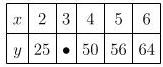
\includegraphics[max width=0.2\textwidth]{images/bo_d7fqvdc91nqc7381i9u0_193_1110_1993_163_67_0.jpg}
\end{center}
\hspace*{3em} 

\section*{校本教材}

专题 1 标题

知识框架

(1)

二、 (2)

1. (a)

2. (b)

一、大类知识点

1、小题型

例1  \ding{72}  \ding{72}  \ding{72}  \ding{72}  \ding{72} 

微信公众号《觅宁参考》制作 微信公众号《觅宁参考》制作 微信公众号《觅宁参考》制作 微信公众号《觅宁参考》制作 微信公众号《觅宁参考》制作 微信公众号 《觅宁参考》制作 微信公众号《觅宁参考》制作 ( )

A. B. C. D.

【简要答案】

练 1.1 微信公众号《觅宁参考》制作 微信公众号《觅宁参考》制作 微信公众号《觅宁参考》制作 微信公众号《觅宁参考》制作 微信公众号《觅宁参考》制作 微信公众号《觅宁参考》制作 微信公众号《觅宁参考》制作 ( )

A. D.

【简要答案】

知识总结

微信公众号《觅宁参考》制作 微信公众号《觅宁参考》制作 微信公众号《觅宁参考》制作 微信公众号《觅宁参考》制作 微信公众号

号《觅宁参考》制作 微信公众号《觅 《觅宁参考》制作 微信公众号《觅宁参考》制作

抛物线知识清单

\section*{【知识清单】}

一、概念性质

定义 平面内与一个定点 \(F\) 和一条定直线 \(l\left( l\right.\) 不经过点 \(F\) ) 距离相等的点的轨迹叫做抛物线. 点 \(F\) 叫做抛物线的焦点,直线 \(l\) 叫做抛物线的 准线.

\section*{几何性质}

\begin{center}
\adjustbox{max width=\textwidth}{
\begin{tabular}{|c|c|c|c|c|}
\hline
标准方程 \(\left( {p > 0}\right)\) & \({y}^{2} = {2px}\) & \({y}^{2} =  - {2px}\) & \({x}^{2} = {2py}\) & \({x}^{2} =  - {2py}\) \\
\cline{1-5}
图象 & 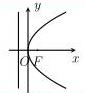
\includegraphics[max width=0.2\textwidth]{images/bo_d7fqvdc91nqc7381i9u0_194_374_1510_85_93_0.jpg} & 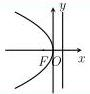
\includegraphics[max width=0.2\textwidth]{images/bo_d7fqvdc91nqc7381i9u0_194_483_1510_90_94_0.jpg} & 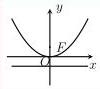
\includegraphics[max width=0.2\textwidth]{images/bo_d7fqvdc91nqc7381i9u0_194_587_1512_100_89_0.jpg} & 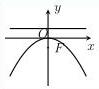
\includegraphics[max width=0.2\textwidth]{images/bo_d7fqvdc91nqc7381i9u0_194_699_1512_99_89_0.jpg} \\
\cline{1-5}
开口方向 & 向右 & 向左 & 向上 & 向下 \\
\cline{1-5}
焦点坐标 & \(P\left( {\frac{p}{2},0}\right)\) & \(P\left( {-\frac{p}{2},0}\right)\) & \(P\left( {0,\frac{p}{2}}\right)\) & \(P\left( {0, - \frac{p}{2}}\right)\) \\
\cline{1-5}
准线方程 & \(x =  - \frac{p}{2}\) & \(x = \frac{p}{2}\) & \(y =  - \frac{p}{2}\) & \(y = \frac{p}{2}\) \\
\cline{1-5}
对称轴 & \multicolumn{2}{|c|}{\(y = 0\)} & \multicolumn{2}{|c|}{\(x = 0\)} \\
\cline{1-5}
顶点坐标 & \multicolumn{4}{|c|}{\(\left( {0,0}\right)\)} \\
\cline{1-5}
离心率 & \multicolumn{4}{|c|}{\(e = 1\) (到定点与到定直线的距离之比称之为离心率)} \\
\cline{1-5}
\hline
\end{tabular}
}
\end{center}

总结记忆

1. 抛物线方程一定首先转化为标准方程;

2. 焦点与一次项保持一致;

3. 焦点到原点的距离为一次项系数的 \(\frac{1}{4}\)

课后练习

1.

( )

A. B. C. D.

【简要答案】

2.

( )

A. B. C. D.

【简要答案】

二、二级结论

1. 焦点弦 \(\left( {p > 0}\right)\)

\begin{center}
\adjustbox{max width=\textwidth}{
\begin{tabular}{|c|c|c|c|c|}
\hline
标准方程 & \({y}^{2} = {2px}\) & \({y}^{2} =  - {2px}\) & \({x}^{2} = {2py}\) & \({x}^{2} =  - {2py}\) \\
\cline{1-5}
焦点弦韦达定理 & \multicolumn{2}{|c|}{\({y}_{1}{y}_{2} =  - {p}^{2},{x}_{1}{x}_{2} = \frac{{p}^{2}}{4}\)} & \multicolumn{2}{|c|}{\({x}_{1}{x}_{2} =  - {p}^{2},{y}_{1}{y}_{2} = \frac{{p}^{2}}{4}\)} \\
\cline{1-5}
焦半径与坐标 & \({x}_{0} + \frac{p}{2}\) & \(- {x}_{0} + \frac{p}{2}\) & \({y}_{0} + p\) & \(- {y}_{0} + \frac{p}{2}\) \\
\cline{1-5}
焦半径与倾斜角 & \multicolumn{2}{|c|}{\(\left| {AF}\right|  = \frac{p}{1 - \cos \theta },\left| {BF}\right|  = \frac{p}{1 + \cos \theta }\) 点 \(A\) 在 \(x\) 轴上方} & \multicolumn{2}{|c|}{\(\left| {AF}\right|  = \frac{p}{1 - \sin \theta },\left| {AF}\right|  = \frac{p}{1 + \sin \theta }\) 注意焦半径小的分母较大} \\
\cline{1-5}
推论 & \multicolumn{2}{|c|}{以 \({AF}\) (或 \({BF}\) ) 为直径的圆与 \(y\) 轴相切} & \multicolumn{2}{|c|}{以 \({AF}\) (或 \({BF}\) ) 为直径的圆与 \(x\) 轴相切} \\
\cline{1-5}
焦半径与定值 & \multicolumn{4}{|c|}{\(\frac{1}{\left| AF\right| } + \frac{1}{\left| BF\right| }\) 为定值为 \(\frac{2}{p}\)} \\
\cline{1-5}
焦点弦长与坐标 & \({x}_{1} + {x}_{2} + p\) & \(- {x}_{1} - {x}_{2} + p\) & \({y}_{1} + {y}_{2} + p\) & \(- {y}_{1} - {y}_{2} + p\) \\
\cline{1-5}
焦点弦长与倾斜角 & \multicolumn{2}{|c|}{\(\left| {AB}\right|  = \frac{2p}{{\sin }^{2}\theta }\)} & \multicolumn{2}{|c|}{\(\left| {AB}\right|  = \frac{2p}{{\cos }^{2}\theta }\)} \\
\cline{1-5}
通径 & \multicolumn{4}{|c|}{最短的焦点弦为通径长为 \({2p}\)} \\
\cline{1-5}
\({S}_{\bigtriangleup {OAB}}\) & \multicolumn{2}{|c|}{\(\frac{{p}^{2}}{2\sin \theta }\)} & \multicolumn{2}{|c|}{\(\frac{{p}^{2}}{2\cos \theta }\)} \\
\cline{1-5}
推论 & \multicolumn{4}{|c|}{以 \({AB}\) 为直径的圆与准线相切,记切点为 \(P\) ,则 \(\angle {APB} = {90}^{ \circ  }\)} \\
\cline{1-5}
\hline
\end{tabular}
}
\end{center}

2. 中点弦

\({y}^{2} = {2px}\) 与 \(y = {kx} + b\) 交于 \(A,B\) 两点,记 \({AB}\) 中点为 \(\left( {{x}_{0},{y}_{0}}\right)\) ,则有 \(\underline{k{y}_{0} = p}\) ; \({x}^{2} = {2py}\) 与 \(y = {kx} + b\) 交于 \(A,B\) 两点,记 \({AB}\) 中点为 \(\left( {{x}_{0},{y}_{0}}\right)\) ,则有 \(\frac{1}{k}{x}_{0} = p\) ;

\section*{幻灯片}

二、探究新知，动手操作

(一)探究新知，回顾背景

\begin{center}
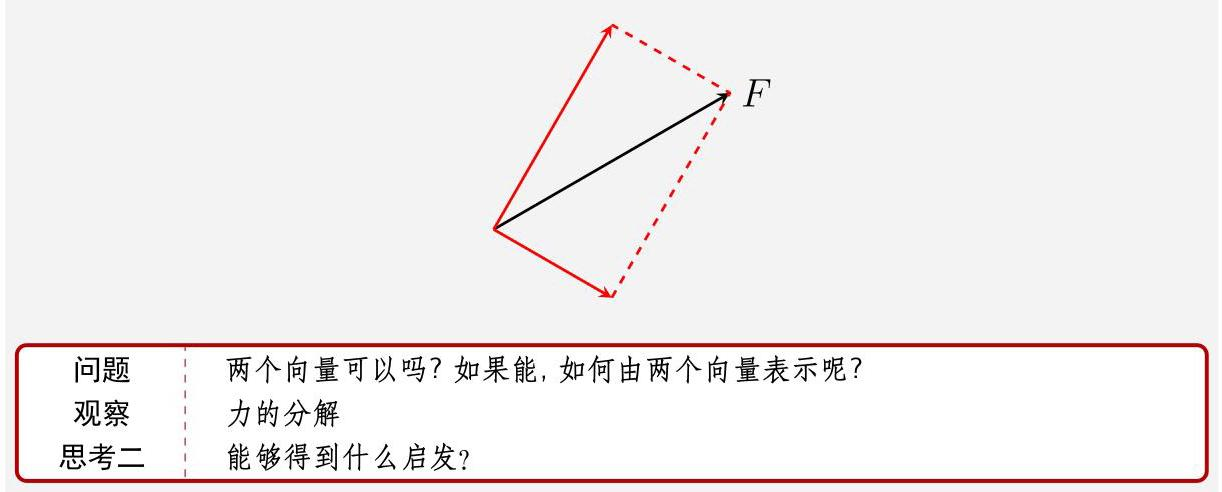
\includegraphics[max width=1.0\textwidth]{images/bo_d7fqvdc91nqc7381i9u0_195_215_416_1222_492_0.jpg}
\end{center}
\hspace*{3em} 

觅宁参考 §6.3.1 平面向量基本定理 3 / 11

二、探究新知，动手操作

(一) 探究新知, 回顾背景

\begin{center}
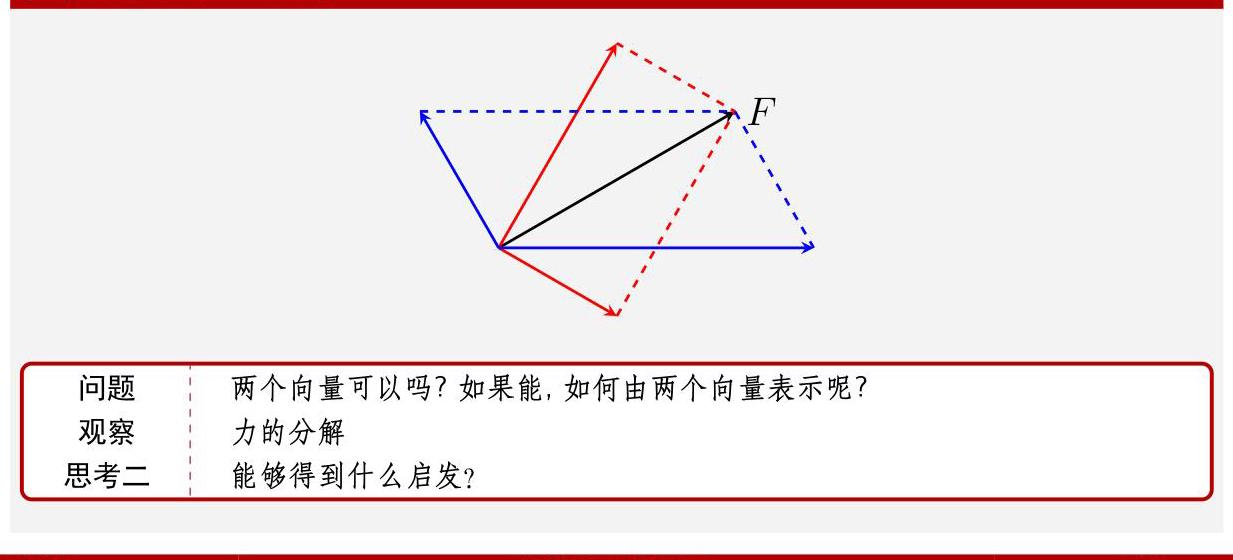
\includegraphics[max width=1.0\textwidth]{images/bo_d7fqvdc91nqc7381i9u0_195_210_1109_1233_560_0.jpg}
\end{center}
\hspace*{3em} 

1. IATEX 本身都可以画出高清矢量图, 同时图中的元素也可以轻松实现逐步显示;

2. 类似地, 图中的文字、公式也可以轻松实现逐步显示, 并且自动对齐;

3. 公式中的数字等实现逐步显示是其他很多软件无法实现的.

\section*{二、探究新知, 动手操作}

(二) 探究新知, 动手操作

\begin{center}
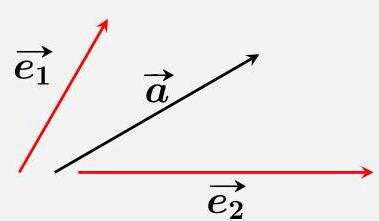
\includegraphics[max width=0.3\textwidth]{images/bo_d7fqvdc91nqc7381i9u0_196_402_367_379_221_0.jpg}
\end{center}
\hspace*{3em} 

\begin{center}
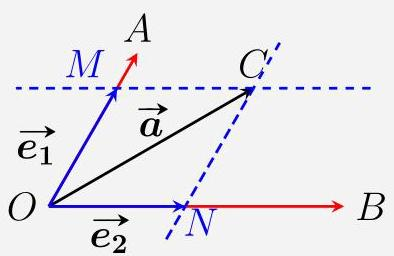
\includegraphics[max width=0.3\textwidth]{images/bo_d7fqvdc91nqc7381i9u0_196_845_333_394_256_0.jpg}
\end{center}
\hspace*{3em} 

\[
\overrightarrow{OC} = \overrightarrow{OM} + \overrightarrow{ON}
\]

\[
\overrightarrow{OM} = {\lambda }_{1}\overrightarrow{OA},\overrightarrow{ON} = {\lambda }_{2}\overrightarrow{OB},
\]

\[
\overrightarrow{OC} = {\lambda }_{1}\overrightarrow{OA} + {\lambda }_{2}\overrightarrow{OB}
\]

\begin{itemize}\relax
\item\relax GeoGebra 动态演示
\end{itemize}

觅宁参考 §6.3.1 平面向量基本定理

裂项相消的一般步骤

例 1

已知数列 \({b}_{n} = \frac{2}{\left( {{2n} - 1}\right) \left( {{2n} + 1}\right) }\) ,求其前 \(n\) 项和 \({S}_{n}\) .

解答

因为 \({b}_{n} = \frac{2}{\left( {{2n} - 1}\right) \left( {{2n} + 1}\right) } = \frac{1}{{2n} - 1} - \frac{1}{{2n} + 1}\) , 对通项裂项

所以 \({S}_{n} = {b}_{1} + {b}_{2} + {b}_{3}\cdots  + {b}_{n - 1} + {b}_{n}\) 求谁表示谁

\(= \left( {\frac{1}{1} - \frac{1}{3}}\right)  + \left( {\frac{1}{3} - \frac{1}{5}}\right)  + \left( {\frac{1}{5} - \frac{1}{7}}\right)  + \cdots  + \left( {\frac{1}{{2n} - 3} - \frac{1}{{2n} - 1}}\right)  + \left( {\frac{1}{{2n} - 1} - \frac{1}{{2n} + 1}}\right)\) 代进去

\(= 1 - \frac{1}{{2n} + 1}\) 消去

\(= \frac{2n}{{2n} + 1}\) 化简

4. 方便对题干、解答做批注, 可以非常方面的提示、引导学生;

5. 试卷、讲义和幻灯片中的内容可以互相复制粘贴, 无需过多调整, 互相兼容性好.

6. 样式简约美观, 格式自动排版, 教师只需要专注内容, 无需花大量时间到格式调整上, 效率高.

\section*{2.5 数学作图方便、精准、美观与文档浑然一体}

\begin{itemize}\relax
\item\relax 函数图象
\end{itemize}

\begin{center}
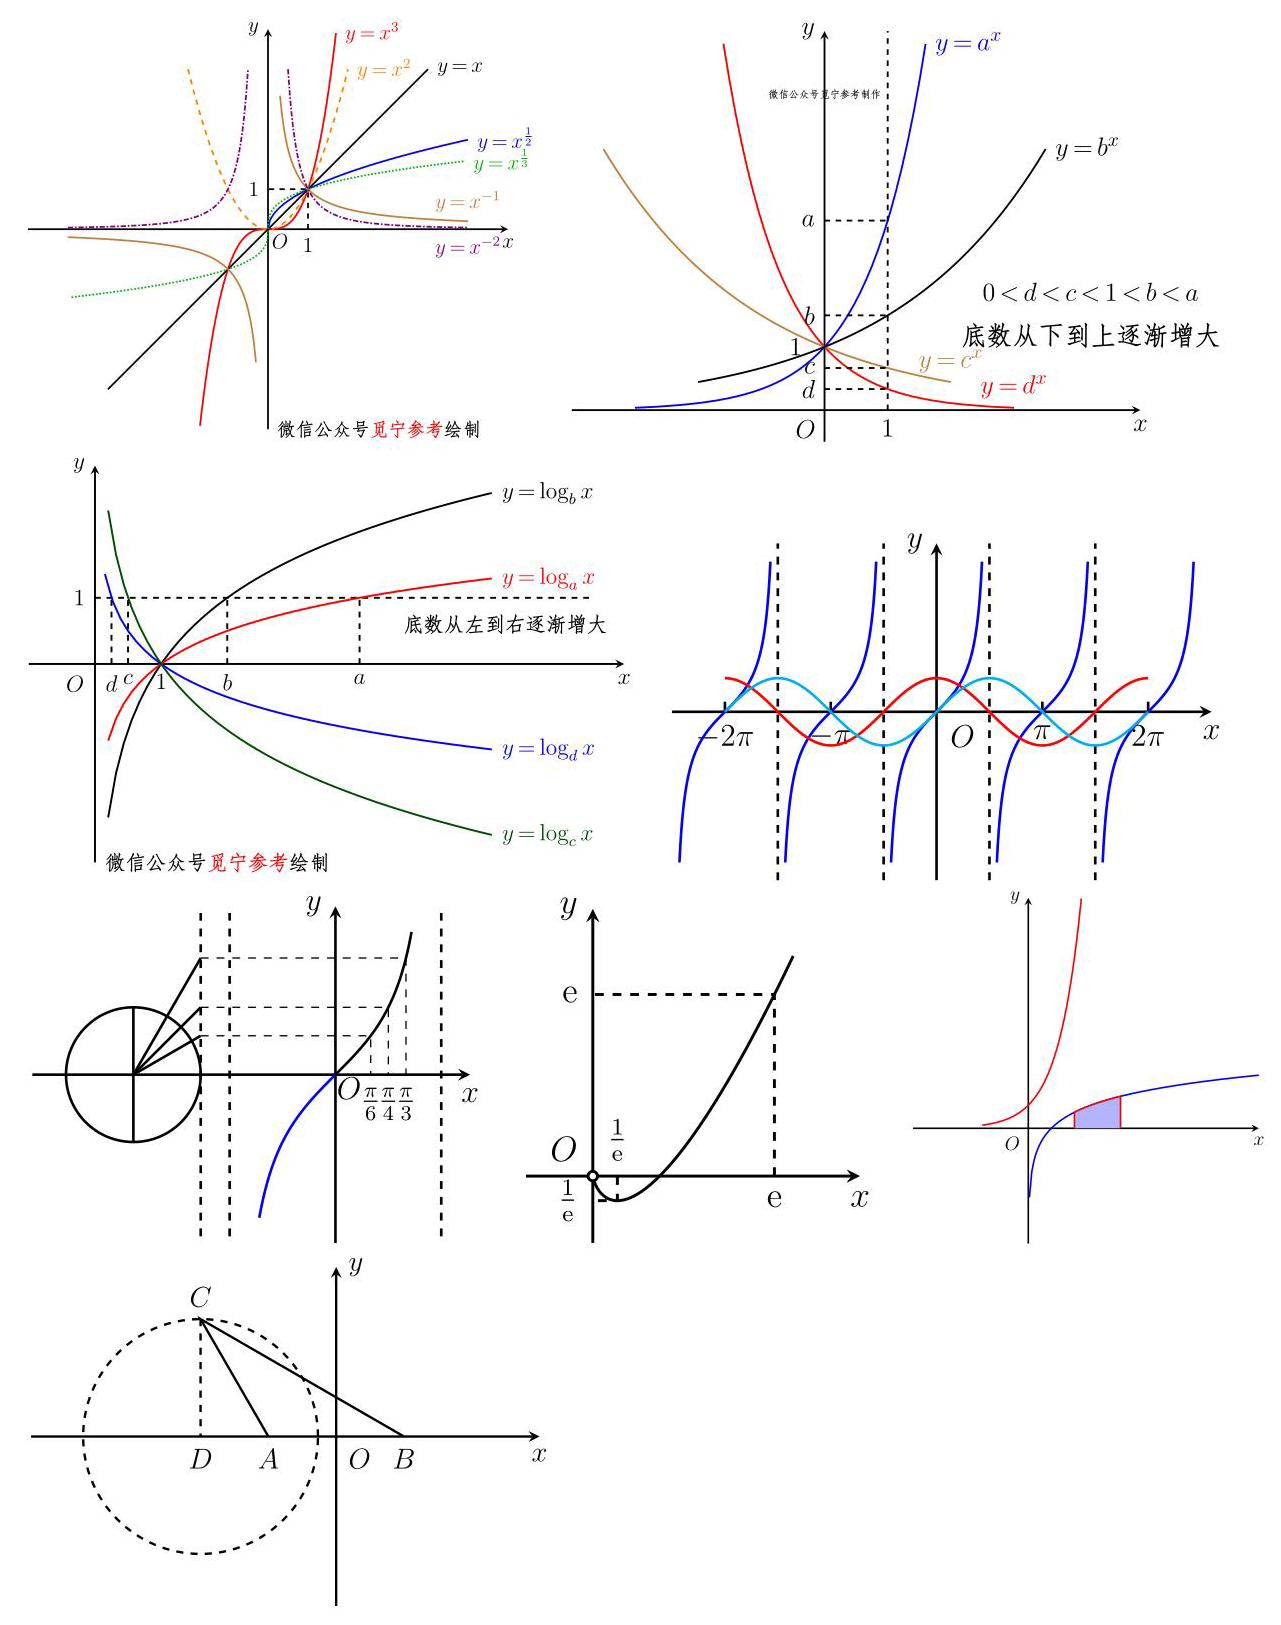
\includegraphics[max width=1.0\textwidth]{images/bo_d7fqvdc91nqc7381i9u0_197_238_382_1281_1625_0.jpg}
\end{center}
\hspace*{3em} 

+ 立体几何

\begin{center}
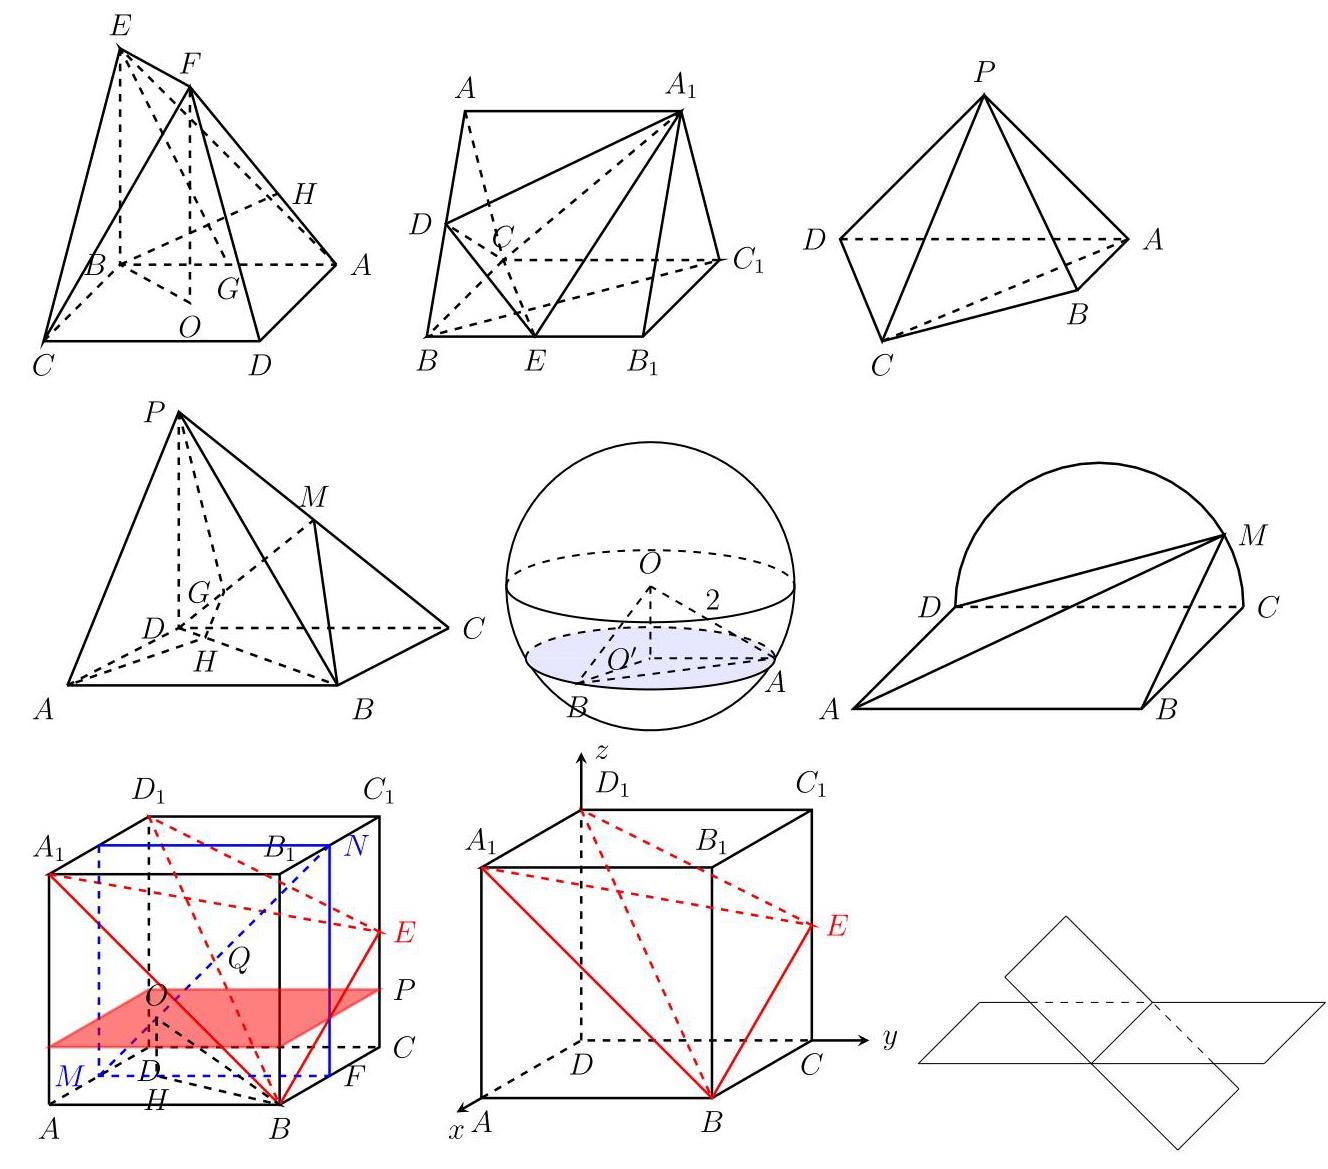
\includegraphics[max width=1.0\textwidth]{images/bo_d7fqvdc91nqc7381i9u0_198_237_357_1328_1169_0.jpg}
\end{center}
\hspace*{3em} 

统计图

\begin{center}
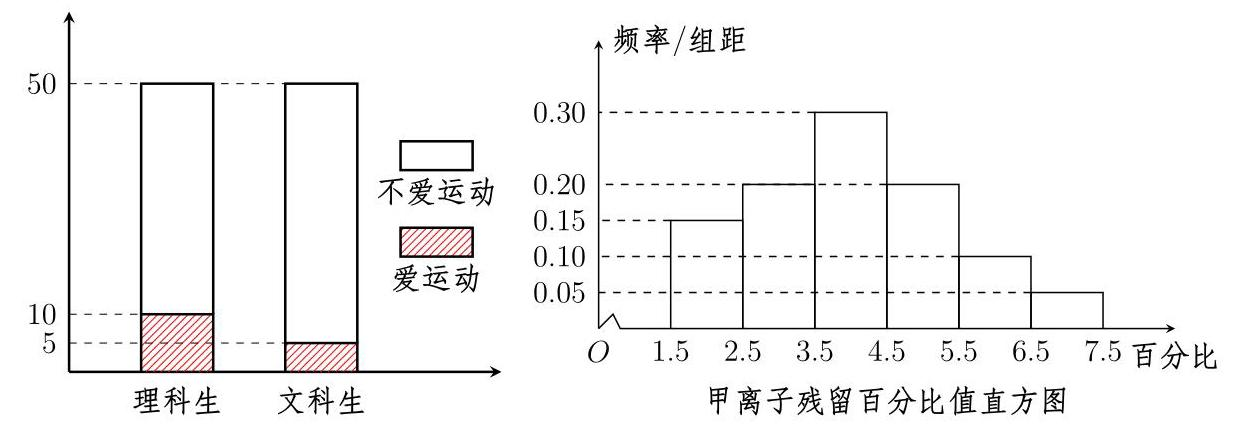
\includegraphics[max width=1.0\textwidth]{images/bo_d7fqvdc91nqc7381i9u0_198_242_1643_1243_433_0.jpg}
\end{center}
\hspace*{3em} 

关注微信公众号《觅宁参考》免费下载软件、教程, 添加微信与作者交流第 13 页 共 20 页

\begin{center}
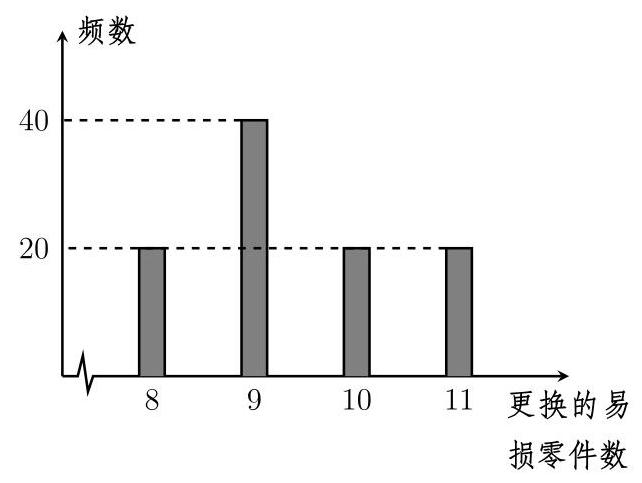
\includegraphics[max width=0.5\textwidth]{images/bo_d7fqvdc91nqc7381i9u0_199_222_295_642_483_0.jpg}
\end{center}
\hspace*{3em} 

\begin{center}
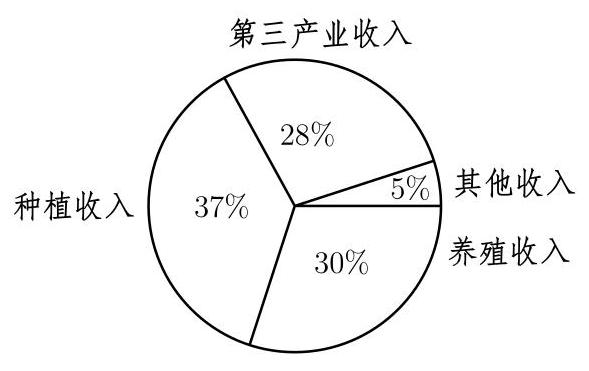
\includegraphics[max width=0.5\textwidth]{images/bo_d7fqvdc91nqc7381i9u0_199_879_333_589_371_0.jpg}
\end{center}
\hspace*{3em} 

建设后经济收入构成比例

\begin{itemize}\relax
\item\relax 圆锥曲线的图
\end{itemize}

\(y\)

-6

\begin{center}
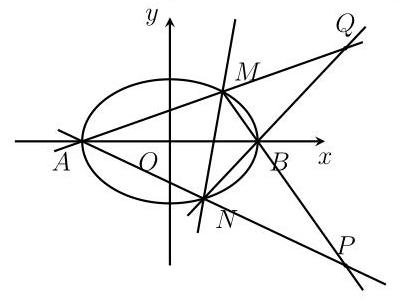
\includegraphics[max width=0.3\textwidth]{images/bo_d7fqvdc91nqc7381i9u0_199_225_1222_398_301_0.jpg}
\end{center}
\hspace*{3em} 

\section*{4 其他平面图形}

\begin{center}
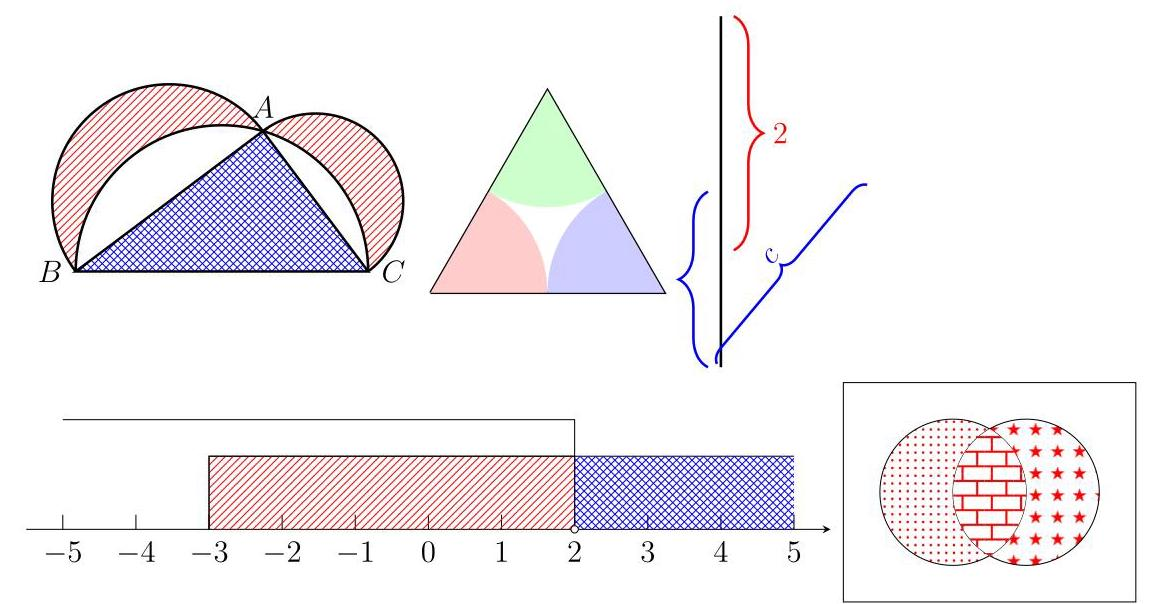
\includegraphics[max width=0.9\textwidth]{images/bo_d7fqvdc91nqc7381i9u0_200_203_347_1154_604_0.jpg}
\end{center}
\hspace*{3em} 

+ 其它图形

\begin{center}
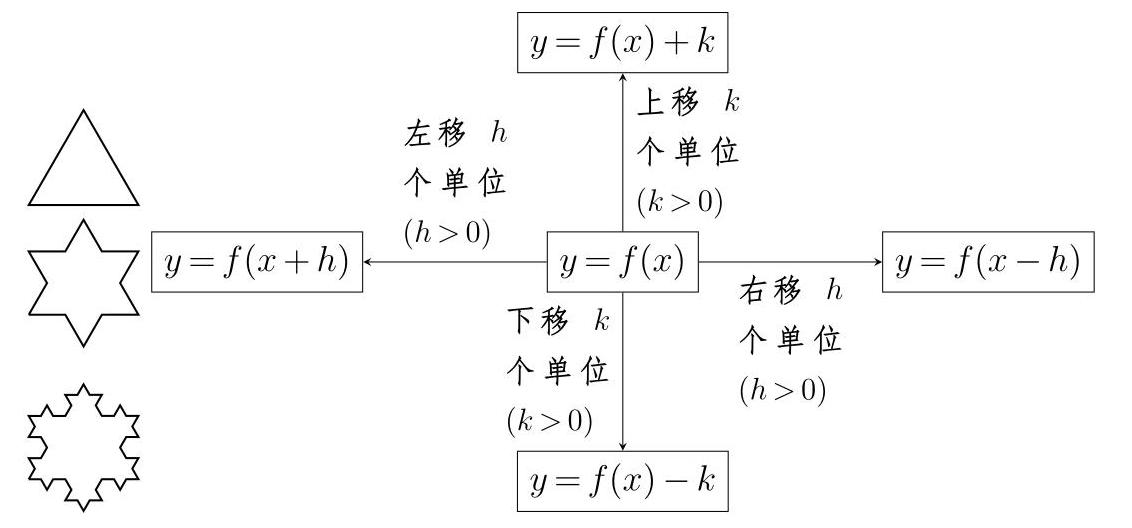
\includegraphics[max width=0.9\textwidth]{images/bo_d7fqvdc91nqc7381i9u0_200_201_1085_1132_528_0.jpg}
\end{center}
\hspace*{3em} 

+ 三视图

\begin{center}
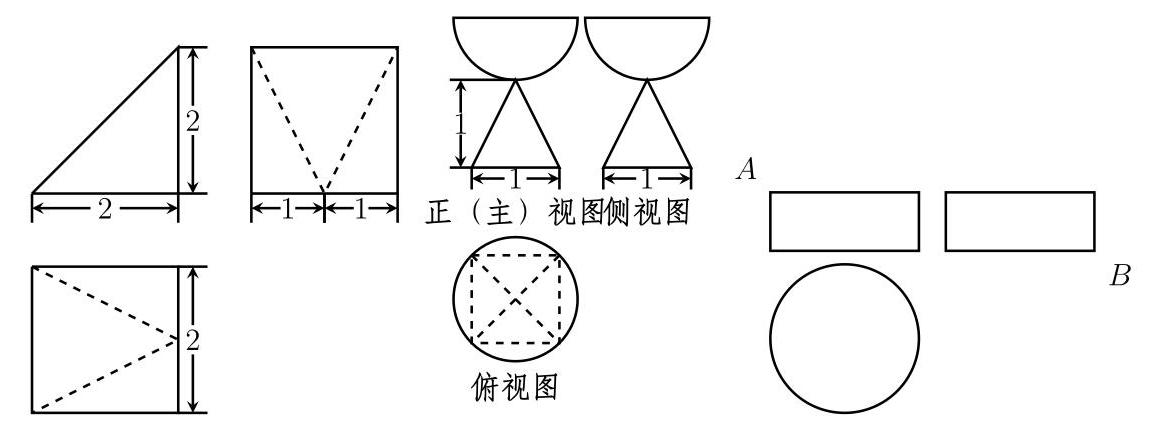
\includegraphics[max width=0.9\textwidth]{images/bo_d7fqvdc91nqc7381i9u0_200_198_1728_1150_428_0.jpg}
\end{center}
\hspace*{3em} 

\section*{与文档浑然一体}

\section*{三、指对幂的函数图象}

\section*{例 6 \(\left( {\bigstar \bigstar \text{  \ding{73}  }\text{  \ding{73}  }\text{  \ding{73}  }}\right)\)}

已知 \({y}_{1} = {\left( \frac{1}{3}\right) }^{x},{y}_{2} = {3}^{x},{y}_{3} = {10}^{-x},{y}_{4} = {10}^{x}\) ,则在同一直角坐标系内,他们的图象为 ( )

\begin{center}
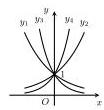
\includegraphics[max width=0.2\textwidth]{images/bo_d7fqvdc91nqc7381i9u0_201_321_371_104_110_0.jpg}
\end{center}
\hspace*{3em} 

A

\begin{center}
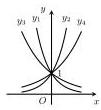
\includegraphics[max width=0.2\textwidth]{images/bo_d7fqvdc91nqc7381i9u0_201_453_372_101_110_0.jpg}
\end{center}
\hspace*{3em} 

B

\begin{center}
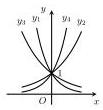
\includegraphics[max width=0.2\textwidth]{images/bo_d7fqvdc91nqc7381i9u0_201_582_372_103_110_0.jpg}
\end{center}
\hspace*{3em} 

C

\begin{center}
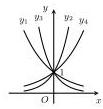
\includegraphics[max width=0.2\textwidth]{images/bo_d7fqvdc91nqc7381i9u0_201_709_373_103_109_0.jpg}
\end{center}
\hspace*{3em} 

D

练 6 ( \ding{72}  \ding{72}  \ding{72}  \ding{73}  \ding{73} )

已知 \(0 < m < n < 1\) ，则指数函数 \(\text{  \circled{1}  }y = {m}^{x}\) ， \(\text{  \circled{2}  }y = {n}^{x}\) 的图象是 ( )

\begin{center}
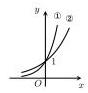
\includegraphics[max width=0.2\textwidth]{images/bo_d7fqvdc91nqc7381i9u0_201_330_574_88_93_0.jpg}
\end{center}
\hspace*{3em} 

A

\begin{center}
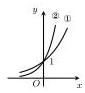
\includegraphics[max width=0.2\textwidth]{images/bo_d7fqvdc91nqc7381i9u0_201_461_574_85_93_0.jpg}
\end{center}
\hspace*{3em} 

B

\begin{center}
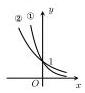
\includegraphics[max width=0.2\textwidth]{images/bo_d7fqvdc91nqc7381i9u0_201_591_574_85_93_0.jpg}
\end{center}
\hspace*{3em} 

C

\begin{center}
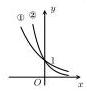
\includegraphics[max width=0.2\textwidth]{images/bo_d7fqvdc91nqc7381i9u0_201_718_575_87_92_0.jpg}
\end{center}
\hspace*{3em} 

D

例 7 \(\left( {x + {\Delta t}{\Delta \phi }}\right)\)

如图所示的曲线是对数函数 \(y = {\log }_{a}x,y = {\log }_{b}x,y = {\log }_{c}x,y = {\log }_{d}x\) 的图象, 则 \(a,b,c,d\) 与 1 的大小关系为 ( )

\begin{center}
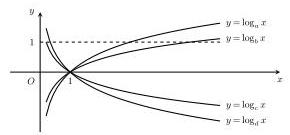
\includegraphics[max width=0.2\textwidth]{images/bo_d7fqvdc91nqc7381i9u0_201_432_789_290_135_0.jpg}
\end{center}
\hspace*{3em} 

A. \(1 < d < c < a < b\) B. \(c < d < 1 < a < b\)

C. \(c < d < 1 < b < a\) D. \(d < c < 1 < a < b\)

练 7 ( \ding{72}  \ding{72}  \ding{72}  \ding{73}  \ding{73} )

已知 \(a > 0,b > 0\) ,且 \({ab} = 1,a \neq  1\) ,则函数 \(f\left( x\right)  = {a}^{x}\) 与函数 \(g\left( x\right)  =  - {\log }_{b}x\) 在

同一坐标系中的图象可能是 ( )

\begin{center}
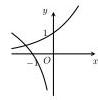
\includegraphics[max width=0.2\textwidth]{images/bo_d7fqvdc91nqc7381i9u0_201_918_273_98_100_0.jpg}
\end{center}
\hspace*{3em} 

A

\begin{center}
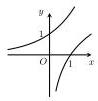
\includegraphics[max width=0.2\textwidth]{images/bo_d7fqvdc91nqc7381i9u0_201_1051_272_98_101_0.jpg}
\end{center}
\hspace*{3em} 

B

\begin{center}
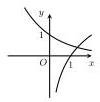
\includegraphics[max width=0.2\textwidth]{images/bo_d7fqvdc91nqc7381i9u0_201_1180_271_100_102_0.jpg}
\end{center}
\hspace*{3em} 

C

\begin{center}
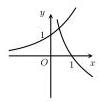
\includegraphics[max width=0.2\textwidth]{images/bo_d7fqvdc91nqc7381i9u0_201_1308_271_99_102_0.jpg}
\end{center}
\hspace*{3em} 

D

例 8 \(\left( {\bigstar \bigstar \text{  \ding{73}  }\text{  \ding{73}  }\text{  \ding{73}  }}\right)\)

如图,幂函数 \(y = {x}^{a},y = {x}^{b},y = {x}^{c},y = {x}^{d}\) 在第一象限内的图象,则 \(a,b,c,d\) 的大小关系为 ( )

\begin{center}
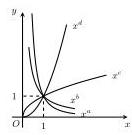
\includegraphics[max width=0.2\textwidth]{images/bo_d7fqvdc91nqc7381i9u0_201_1106_491_132_135_0.jpg}
\end{center}
\hspace*{3em} 

A. \(a < b < c < d\;\) B. \(a < b < d < c\;\) C. \(b < a < c < d\;\) D. \(b < a < d < c\)

练 8 \(\left( {\phi  \star  \phi  \star  \phi  \star  \phi }\right)\)

函数 \(y = \frac{1}{x},y = x,y = 1\) 的图象和直线 \(x = 1\) 将平面直角坐标系的第一象限分为 8 个部分: \circled{1}  \circled{2}  \circled{3}  \circled{4}  \circled{5}  \circled{6}  \circled{7}  \circled{8} ，若幂函数 \(f\left( x\right)\) 的图象经过的部分是 \circled{4}  \circled{8} ，则 \(f\left( x\right)\) 可能是 ( )

\begin{center}
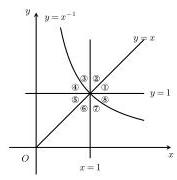
\includegraphics[max width=0.2\textwidth]{images/bo_d7fqvdc91nqc7381i9u0_201_1083_784_177_180_0.jpg}
\end{center}
\hspace*{3em} 

A. \(y = {x}^{2}\) B. \(y = \frac{1}{\sqrt{x}}\) C. \(y = {x}^{\frac{1}{2}}\) D. \(y = {x}^{-2}\)

1、根据平移、对称、翻折和伸缩变换画图

例 1 已知 \(f\left( x\right)  = \ln x\) ,画出下列函数的图象

(1) \(y = f\left( {x - 1}\right)\) (2) \(y = f\left( x\right)  + 1\) (3) \(y = f\left( {-x}\right)\)

(4) \(y =  - f\left( x\right)\) (5) \(y = \left| {f\left( x\right) }\right|\) (6) \(y = f\left( \left| x\right| \right)\)

(1)

\begin{center}
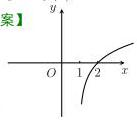
\includegraphics[max width=0.2\textwidth]{images/bo_d7fqvdc91nqc7381i9u0_201_334_1250_137_122_0.jpg}
\end{center}
\hspace*{3em} 

(2)

\begin{center}
\includegraphics[max width=0.2\textwidth]{images/bo_d7fqvdc91nqc7381i9u0_201_517_1250_127_122_0.jpg}
\end{center}
\hspace*{3em} 

(3)

\begin{center}
\includegraphics[max width=0.2\textwidth]{images/bo_d7fqvdc91nqc7381i9u0_201_693_1250_132_121_0.jpg}
\end{center}
\hspace*{3em} 

(4)

\begin{center}
\includegraphics[max width=0.2\textwidth]{images/bo_d7fqvdc91nqc7381i9u0_201_335_1377_130_124_0.jpg}
\end{center}
\hspace*{3em} 

(5)

\begin{center}
\includegraphics[max width=0.2\textwidth]{images/bo_d7fqvdc91nqc7381i9u0_201_516_1376_129_126_0.jpg}
\end{center}
\hspace*{3em} 

(6)

\begin{center}
\includegraphics[max width=0.2\textwidth]{images/bo_d7fqvdc91nqc7381i9u0_201_693_1378_131_124_0.jpg}
\end{center}
\hspace*{3em} 

练 1 画出下列函数的图象

(1) \(y = {2}^{x + 1} - 1\)

(4) \(y = \frac{x - 1}{x + 1}\)

(2) \(y = {2}^{-\left| x\right| }\)

(5) \(y = \frac{{2x} + 1}{x - 1}\)

(3) \(y = \left| {{2}^{\left| x\right| } - 2}\right|\)

(6) \(y = \left| {x + 1}\right|\)

【答案】

\begin{center}
\includegraphics[max width=0.2\textwidth]{images/bo_d7fqvdc91nqc7381i9u0_201_333_1598_125_121_0.jpg}
\end{center}
\hspace*{3em} 

(1)

(2)

\begin{center}
\includegraphics[max width=0.2\textwidth]{images/bo_d7fqvdc91nqc7381i9u0_201_516_1594_120_123_0.jpg}
\end{center}
\hspace*{3em} 

(3)

\begin{center}
\includegraphics[max width=0.2\textwidth]{images/bo_d7fqvdc91nqc7381i9u0_201_694_1594_121_123_0.jpg}
\end{center}
\hspace*{3em} 

(4)

\begin{center}
\includegraphics[max width=0.2\textwidth]{images/bo_d7fqvdc91nqc7381i9u0_201_334_1721_169_169_0.jpg}
\end{center}
\hspace*{3em} 

\begin{center}
\includegraphics[max width=0.2\textwidth]{images/bo_d7fqvdc91nqc7381i9u0_201_514_1720_164_169_0.jpg}
\end{center}
\hspace*{3em} 

\begin{center}
\includegraphics[max width=0.2\textwidth]{images/bo_d7fqvdc91nqc7381i9u0_201_691_1751_166_141_0.jpg}
\end{center}
\hspace*{3em} 

\section*{2、根据函数的性质画图}

例 2 画出下列函数的图象

(1)

\begin{center}
\includegraphics[max width=0.2\textwidth]{images/bo_d7fqvdc91nqc7381i9u0_201_923_1196_177_184_0.jpg}
\end{center}
\hspace*{3em} 

(2) \(f\left( x\right)  = x + \ln x\) ;

(2)

\begin{center}
\includegraphics[max width=0.2\textwidth]{images/bo_d7fqvdc91nqc7381i9u0_201_1208_1227_104_154_0.jpg}
\end{center}
\hspace*{3em} 

练 2 已知奇函数 \(f\left( x\right)\) 定义域为 \(\mathbf{R}\) ,当 \(x \in  \left\lbrack  {0,1}\right\rbrack\) 时, \(f\left( x\right)  = x\) ,且 \(f\left( x\right)\) 的图象关于 \(x = 1\) 对称,画出 \(f\left( x\right)\) 在 \(\left\lbrack  {-5,5}\right\rbrack\) 的函数图象.

【答案】

\begin{center}
\includegraphics[max width=0.2\textwidth]{images/bo_d7fqvdc91nqc7381i9u0_201_964_1462_276_106_0.jpg}
\end{center}
\hspace*{3em} 

\section*{3、复杂函数运用导数画图}

例 3 画出下列函数的图象

\begin{center}
\includegraphics[max width=0.2\textwidth]{images/bo_d7fqvdc91nqc7381i9u0_201_1291_1620_116_177_0.jpg}
\end{center}
\hspace*{3em} 

(1) \(y = x\ln x\)

(2) \(y = \frac{\ln x}{x}\)

\begin{center}
\includegraphics[max width=0.2\textwidth]{images/bo_d7fqvdc91nqc7381i9u0_201_1116_1636_154_163_0.jpg}
\end{center}
\hspace*{3em} 

(3)

(3)

\begin{center}
\includegraphics[max width=0.2\textwidth]{images/bo_d7fqvdc91nqc7381i9u0_201_905_1648_180_135_0.jpg}
\end{center}
\hspace*{3em} 

\(f\left( x\right)  = x\ln x\)

(2) (1)

1. 图的细节均可直接修改, 整体效果与文档本身浑然一体.

2. 选项可以根据图的大小, 自动排列一行四个或两个或一个, 图可以居中、居右或居左.

\section*{三、课程简介与学习流程}

目前全部课程大约有 40 课时的视频，包括四方面内容，分别为:试卷编辑基础模块、讲义编辑提高模块、画图模版、幻灯片制作模版. 除此之外, 也会将学员经常遇到的问题解答制作成视频上传, 90\% 的老师都可以根据视频学习掌握, 对于在学习中有疑惑的地方, 还会提供答疑, 远程协助解决问题, 确保参与课程的学员完成学习目标, 能够独立编辑出试卷、讲义等文档. 课程目标与教学内容见附件.

\section*{课程形式}

课程包括视频课程、文档资料和若干次答疑, 其中视频课程为在线视频, 可以回放, 老师们可以根据自己的时间安排学习, 同时参考提供的文档资料, 对于有疑问的地方, 会通过微信或者远程提供答疑, 这样的教学方式,符合学习规律,节约时间,效率高,比自学节约 90\% 的时间,参加课程快则一天，慢则一周即可独立排版一份试卷、讲义。

\section*{电脑基础}

学习软件所需要的电脑基础:会打字，大多数情况能够打字不看键盘。 课程是面向零基础的中学老师, 不需要额外的编程基础.

\section*{学习流程}

1. 报名参加课程、安装软件、配置软件, 浏览课程所发资料, 知道资料都有哪些内容;

2. 认真观看前五个视频, 认真操作;

3. 尝试排版一份高考试卷, 遇到问题, 先查看视频和代码手册, 如果不能解决, 微信联系我即可.

4. 后期根据自己需求, 选择性的学习视频课程.

未尽事宜，可微信交流.

\section*{附件: 公式效果}

基本符号

希腊字母

集合

\begin{center}
\includegraphics[max width=0.2\textwidth]{images/bo_d7fqvdc91nqc7381i9u0_203_1068_1473_178_444_0.jpg}
\end{center}
\hspace*{3em} 

\begin{center}
\adjustbox{max width=\textwidth}{
\begin{tabular}{|c|c|c|}
\hline
\phantom{X} & 序号 & 符号 \\
\cline{1-3}
\phantom{X} & 1. & \(\sqrt{2},\sqrt[3]{3},\sqrt{\frac{1}{2}}\) \\
\cline{1-3}
\phantom{X} & 2. & \(\frac{2}{3},\frac{\sqrt{3}}{2}\) \\
\cline{1-3}
\phantom{X} & 3. & \(\overrightarrow{AB},\mathbf{a}\) \\
\cline{1-3}
\phantom{X} & 4. & \(\bar{a},\widehat{a},\overline{1234}\) \\
\cline{1-3}
\phantom{X} & 5. & \({a}_{m},{a}^{n},{a}_{n + 1}^{n + 2}\) \\
\cline{1-3}
\phantom{X} & 6. & \{\} \\
\cline{1-3}
\phantom{X} & 7. & \% \\
\cline{1-3}
\phantom{X} & 8. & \(+ \infty , - \infty\) \\
\cline{1-3}
\phantom{X} & 9. & \(\because \therefore\) \\
\cline{1-3}
\phantom{X} & 10. & \(\langle \mathbf{a},\mathbf{b}\rangle\) \\
\cline{1-3}
\phantom{X} & 11. & \(\int\) \\
\cline{1-3}
\phantom{X} & 12. &  \ding{56}  \\
\cline{1-3}
\phantom{X} & 13. & ÷ \\
\cline{1-3}
\phantom{X} & 14. & + \\
\cline{1-3}
\phantom{X} & 15. & < \\
\cline{1-3}
\phantom{X} & 16. & 之 \\
\cline{1-3}
\phantom{X} & 17. & \(\neq\) \\
\cline{1-3}
\phantom{X} & 18. & \(\approx\) \\
\cline{1-3}
\phantom{X} & 19. & ... \\
\cline{1-3}
\phantom{X} & 20. & 十 \\
\cline{1-3}
\phantom{X} & 21. & (mod \(m\) ) \\
\cline{1-3}
\phantom{X} & 22. & 着重号 \\
\cline{1-3}
\phantom{X} & 23. & 公式中中文 \\
\cline{1-3}
\phantom{X} & 24. & \includegraphics[max width=0.2\textwidth]{images/bo_d7fqvdc91nqc7381i9u0_203_383_2030_60_97_0.jpg} \\
\cline{1-3}
\hline
\end{tabular}
}
\end{center}

\begin{center}
\adjustbox{max width=\textwidth}{
\begin{tabular}{|c|c|c|}
\hline
\phantom{X} & 序号 & 符号 \\
\cline{1-3}
\phantom{X} & 25. & \(\alpha\) \\
\cline{1-3}
\phantom{X} & 26. & \(\beta\) \\
\cline{1-3}
\phantom{X} & 27. & \(\gamma\) \\
\cline{1-3}
\phantom{X} & 28. & \(\delta\) \\
\cline{1-3}
\phantom{X} & 29. & \(\varepsilon\) \\
\cline{1-3}
\phantom{X} & 30. & \(\eta\) \\
\cline{1-3}
\phantom{X} & 31. & \(\theta\) \\
\cline{1-3}
\phantom{X} & 32. & \(\lambda\) \\
\cline{1-3}
\phantom{X} & 33. & \(\mu\) \\
\cline{1-3}
\phantom{X} & 34. & \(\nu\) \\
\cline{1-3}
\phantom{X} & 35. & \(\xi\) \\
\cline{1-3}
\phantom{X} & 36. & \(\pi\) \\
\cline{1-3}
\phantom{X} & 37. & \(\rho\) \\
\cline{1-3}
\phantom{X} & 38. & \(\sigma\) \\
\cline{1-3}
\phantom{X} & 39. & \(\varphi\) \\
\cline{1-3}
\phantom{X} & 40. & \(\omega\) \\
\cline{1-3}
\phantom{X} & 41. & \(\Delta\) \\
\cline{1-3}
\phantom{X} & 42. & \(\Omega\) \\
\cline{1-3}
\phantom{X} & 43. & \(\Gamma\) \\
\cline{1-3}
\hline
\end{tabular}
}
\end{center}

\begin{center}
\adjustbox{max width=\textwidth}{
\begin{tabular}{|c|c|}
\hline
序号 & 符号 \\
\cline{1-2}
48. & UU \\
\cline{1-2}
49. & \(\cap   \cap\) \\
\cline{1-2}
50. & 三 \\
\cline{1-2}
51. & 三 \\
\cline{1-2}
52. & 字 \\
\cline{1-2}
53. & \({\complement }_{U}A\) \\
\cline{1-2}
54. & \(\in   \notin\) \\
\cline{1-2}
55. & \(\varnothing\) \\
\cline{1-2}
56. & \(\otimes\) \\
\cline{1-2}
57. & \(\oplus\) \\
\cline{1-2}
58. & ※ \\
\cline{1-2}
59. & \(\neg p\) \\
\cline{1-2}
60. & \(p \vee  q\) \\
\cline{1-2}
61. & \(p \land  q\) \\
\cline{1-2}
62. & \(\exists \forall\) \\
\cline{1-2}
\hline
\end{tabular}
}
\end{center}

卷

\begin{center}
\adjustbox{max width=\textwidth}{
\begin{tabular}{|c|c|c|c|}
\hline
\multicolumn{4}{|c|}{大型运算符号} \\
\cline{1-4}
\phantom{X} & 44. & \(\mathop{\sum }\limits_{{i = 1}}^{n}\) & \phantom{X} \\
\cline{1-4}
\phantom{X} & 45. & \(\mathop{\prod }\limits_{{i = 1}}^{n}\) & \phantom{X} \\
\cline{1-4}
\phantom{X} & 46. & \({\int }_{1}^{n}\) & \phantom{X} \\
\cline{1-4}
\phantom{X} & 47. & \makecell{ lim \\ \(x \rightarrow   + \infty\) } & \phantom{X} \\
\cline{1-4}
\hline
\end{tabular}
}
\end{center}

判断对错

\begin{center}
\adjustbox{max width=\textwidth}{
\begin{tabular}{|c|c|}
\hline
69. & \phantom{X} \\
\cline{1-2}
70. & \phantom{X} \\
\cline{1-2}
\hline
\end{tabular}
}
\end{center}

几何

\begin{center}
\adjustbox{max width=\textwidth}{
\begin{tabular}{|c|c|}
\hline
序号 & 符号 \\
\cline{1-2}
71. & ⊥ \\
\cline{1-2}
72. & 丨 \\
\cline{1-2}
73. & \(\bigtriangleup\) \\
\cline{1-2}
74. &  \circled{2}  \\
\cline{1-2}
75. & L \\
\cline{1-2}
76. & \(□\) \\
\cline{1-2}
77. & // \\
\cline{1-2}
78. & ～ \\
\cline{1-2}
79. & 了 \\
\cline{1-2}
80. & ≅ \\
\cline{1-2}
81. & 19 \\
\cline{1-2}
82. & \(\overset{\text{ ⏜ }}{AB}\) \\
\cline{1-2}
\hline
\end{tabular}
}
\end{center}

难度选择填空

\[
f\left( x\right)  = \left\{  {\begin{array}{l} {x}^{2} - {2x} + 3,x \leq  1, \\  x - 2,x > 1, \end{array}\;f\left( x\right)  = \left\{  \begin{array}{ll} {x}^{2} - {2x} + 3, & x \leq  1, \\  x - 2, & x > 1, \end{array}\right. }\right.
\]

\begin{center}
\adjustbox{max width=\textwidth}{
\begin{tabular}{|c|c|c|}
\hline
\phantom{X} & 83. &  \ding{72}  \ding{73}  \ding{73}  \ding{73}  \ding{73}  \\
\cline{1-3}
\phantom{X} & 84. &  \ding{72}  \ding{72}  \ding{73}  \ding{73}  \ding{73}  \\
\cline{1-3}
\phantom{X} & 85. &  \ding{72}  \ding{72}  \ding{72}  \ding{73}  \ding{73}  \\
\cline{1-3}
\phantom{X} & 86. &  \ding{72}  \ding{72}  \ding{72}  \ding{72}  \ding{73}  \\
\cline{1-3}
\phantom{X} & 87. &  \ding{72}  \ding{72}  \ding{72}  \ding{72}  \ding{72}  \\
\cline{1-3}
\phantom{X} & 88. &  \ding{73}  \ding{73}  \ding{73}  \ding{73}  \ding{73}  \\
\cline{1-3}
\phantom{X} & 89. &  \ding{72}  \ding{72}  \ding{72}  \ding{73}  \ding{73}  \\
\cline{1-3}
\phantom{X} & 90. & ( ) \\
\cline{1-3}
\phantom{X} & 91. & \_\_\_\_\_ \\
\cline{1-3}
\phantom{X} & 92. & \_\_\_\_\_ \\
\cline{1-3}
\hline
\end{tabular}
}
\end{center}

\begin{center}
\adjustbox{max width=\textwidth}{
\begin{tabular}{|c|c|c|}
\hline
\multicolumn{3}{|c|}{函数} \\
\cline{1-3}
\multirow{13}{*}{\phantom{X}} & 序号 & 符号 \\
\cline{2-3}
 & 93. & \(\lim x\) \\
\cline{2-3}
 & 94. & \(\cos x\) \\
\cline{2-3}
 & 95. & \(\sin x\) \\
\cline{2-3}
 & 96. & \(\tan x\) \\
\cline{2-3}
 & 97. & \(\lg x\) \\
\cline{2-3}
 & 98. & \(\ln x\) \\
\cline{2-3}
 & 99. & \(\log x\) \\
\cline{2-3}
 & 100. & \(\max x\) \\
\cline{2-3}
 & 101. & \(\min x\) \\
\cline{2-3}
 & 102. & \(\arccos x\) \\
\cline{2-3}
 & 103. & \(\arcsin x\) \\
\cline{2-3}
 & 104. & \(\arctan x\) \\
\cline{1-3}
\hline
\end{tabular}
}
\end{center}

罗马数字

105. I

106. II

107. III

108. X

109. XV

110. i

111. ii

112. iii

113. X

114. XV

\begin{center}
\adjustbox{max width=\textwidth}{
\begin{tabular}{|c|c|}
\hline
\multicolumn{2}{|c|}{箭头} \\
\cline{1-2}
115. &  \ding{51}  \\
\cline{1-2}
116. & \(\rightarrow\) \\
\cline{1-2}
117. & \(\Leftarrow\) \\
\cline{1-2}
118. & \(\Rightarrow\) \\
\cline{1-2}
119. & ⇔ \\
\cline{1-2}
120. & 今 \\
\cline{1-2}
121. & ↗ \\
\cline{1-2}
122. & ↘ \\
\cline{1-2}
123. & 应 \\
\cline{1-2}
124. &  \ding{51}  \\
\cline{1-2}
125. & \(\uparrow   \downarrow\) \\
\cline{1-2}
126. &  \ding{51}  \\
\cline{1-2}
127. & 一 \\
\cline{1-2}
128. & 一 \\
\cline{1-2}
129. & 一 \\
\cline{1-2}
130. & \(\Rightarrow\) \\
\cline{1-2}
131. & \(\Leftrightarrow\) \\
\cline{1-2}
132. & 上 \\
\cline{1-2}
133. & 上 \\
\cline{1-2}
134. & 占 \\
\cline{1-2}
135. & 二 \\
\cline{1-2}
\hline
\end{tabular}
}
\end{center}

\section*{公式等号对齐}

\({10} = 1 + 9\)

\[
{10} = 1 + 9
\]

\({10} = 1 + 1 + 8 \; {10} = 1 + 1 + 8\)

\({10} = 1 + 1 + 1 + 7 \; {10} = 1 + 1 + 1 + 7\)

在我们教学、做题的过程中, 有很多好的想法、思路, 但由于没有及时的记录、整理，而逐渐遗忘，即使努力回想，多是徒劳，非常遗憾. 学会 IATEX, 可以方程方便的编辑公式, 画图, 大大提高效率记录我们专业成长的每一步，让每个灵感闪现的时刻不再转瞬即逝！

给大家提供一个决策的角度:一件事是否值得做，当下可能觉得受很多因素影响, 不知道如何取舍的时, 不妨让五年、十年后的自己帮做决策, 十年之后哪些因素才是最重要的, 立刻变得清晰.

一项技能会在时间的作用下, 愈发珍贵, IATEX 这一工具, 方便记录, 平时的积累够了，关键时刻就能迸发无穷的力量，一起加入学习吧.

\section*{一、函数图象}

\begin{center}
\includegraphics[max width=1.0\textwidth]{images/bo_d7fqvdc91nqc7381i9u0_206_129_129_1417_2097_0.jpg}
\end{center}
\hspace*{3em} 

关注微信公众号《觅宁参考》免费下载上述画图软件，添加小编微信，学习公式编辑、画图、下载高中数学专题第 1 页 共 4 页

\section*{二、立体几何}

\begin{center}
\includegraphics[max width=1.0\textwidth]{images/bo_d7fqvdc91nqc7381i9u0_207_161_157_1441_1269_0.jpg}
\end{center}
\hspace*{3em} 

\section*{三、统计图}

\begin{center}
\includegraphics[max width=1.0\textwidth]{images/bo_d7fqvdc91nqc7381i9u0_207_160_1539_1372_478_0.jpg}
\end{center}
\hspace*{3em} 

关注微信公众号《觅宁参考》免费下载上述画图软件，添加小编微信，学习公式编辑、画图、下载高中数学专题

第 2 页 共 4 页

\begin{center}
\includegraphics[max width=0.5\textwidth]{images/bo_d7fqvdc91nqc7381i9u0_208_168_103_677_501_0.jpg}
\end{center}
\hspace*{3em} 

第三产业收入

28\%

种植收入 37\%

5\% 其他收入

30\% 养殖收入

建设后经济收入构成比例

四、圆锥曲线等平面图

\begin{center}
\includegraphics[max width=1.0\textwidth]{images/bo_d7fqvdc91nqc7381i9u0_208_157_735_1481_754_0.jpg}
\end{center}
\hspace*{3em} 

\section*{五、 其他平面图形}

\begin{center}
\includegraphics[max width=0.9\textwidth]{images/bo_d7fqvdc91nqc7381i9u0_208_158_1612_1057_478_0.jpg}
\end{center}
\hspace*{3em} 

关注微信公众号《觅宁参考》免费下载上述画图软件，添加小编微信，学习公式编辑、画图、下载高中数学专题第 3 页 共 4 页

\section*{六、其它图形}

\begin{center}
\includegraphics[max width=1.0\textwidth]{images/bo_d7fqvdc91nqc7381i9u0_209_144_153_1206_565_0.jpg}
\end{center}
\hspace*{3em} 

七、三视图

\begin{center}
\includegraphics[max width=1.0\textwidth]{images/bo_d7fqvdc91nqc7381i9u0_209_148_826_1214_455_0.jpg}
\end{center}
\hspace*{3em} 

\section*{八、流程图}

\begin{center}
\includegraphics[max width=0.7\textwidth]{images/bo_d7fqvdc91nqc7381i9u0_209_153_1388_841_844_0.jpg}
\end{center}
\hspace*{3em} 

关注微信公众号《觅宁参考》免费下载上述画图软件，添加小编微信，学习公式编辑、画图、下载高中数学专题第 4 页 共 4 页

\section*{指对幂图象及其性质}

\section*{一、指对幂的函数图象}

例 1 已知 \({y}_{1} = {\left( \frac{1}{3}\right) }^{x},{y}_{2} = {3}^{x},{y}_{3} = {10}^{-x},{y}_{4} = {10}^{x}\) ,则在同一直角坐标系内,他们的图象为 ( )

\begin{center}
\includegraphics[max width=0.2\textwidth]{images/bo_d7fqvdc91nqc7381i9u0_210_186_296_187_201_0.jpg}
\end{center}
\hspace*{3em} 

A

\begin{center}
\includegraphics[max width=0.2\textwidth]{images/bo_d7fqvdc91nqc7381i9u0_210_449_298_187_199_0.jpg}
\end{center}
\hspace*{3em} 

B

\begin{center}
\includegraphics[max width=0.2\textwidth]{images/bo_d7fqvdc91nqc7381i9u0_210_712_298_187_199_0.jpg}
\end{center}
\hspace*{3em} 

C

\begin{center}
\includegraphics[max width=0.2\textwidth]{images/bo_d7fqvdc91nqc7381i9u0_210_974_299_187_199_0.jpg}
\end{center}
\hspace*{3em} 

D

练 1 已知 \(0 < m < n < 1\) ,则指数函数 \(\text{  \circled{1}  }y = {m}^{x},\text{  \circled{2}  }y = {n}^{x}\) 的图象是 ( )

\begin{center}
\includegraphics[max width=0.2\textwidth]{images/bo_d7fqvdc91nqc7381i9u0_210_202_688_155_169_0.jpg}
\end{center}
\hspace*{3em} 

A

\begin{center}
\includegraphics[max width=0.2\textwidth]{images/bo_d7fqvdc91nqc7381i9u0_210_464_689_155_168_0.jpg}
\end{center}
\hspace*{3em} 

B

\begin{center}
\includegraphics[max width=0.2\textwidth]{images/bo_d7fqvdc91nqc7381i9u0_210_728_689_154_168_0.jpg}
\end{center}
\hspace*{3em} 

C

\begin{center}
\includegraphics[max width=0.2\textwidth]{images/bo_d7fqvdc91nqc7381i9u0_210_990_689_155_168_0.jpg}
\end{center}
\hspace*{3em} 

D

例 2 如图所示的曲线是对数函数 \(y = {\log }_{a}x,y = {\log }_{b}x,y = {\log }_{c}x,y = {\log }_{d}x\) 的图象,则 \(a,b,c,d\) 与 1 的大小关系为 ( )

\begin{center}
\includegraphics[max width=0.3\textwidth]{images/bo_d7fqvdc91nqc7381i9u0_210_377_1093_524_243_0.jpg}
\end{center}
\hspace*{3em} 

A. \(1 < d < c < a < b\) B. \(c < d < 1 < a < b\) C. \(c < d < 1 < b < a\) D. \(d < c < 1 < a < b\)

练 2 已知 \(a > 0,b > 0\) ,且 \({ab} = 1,a \neq  1\) ,则函数 \(f\left( x\right)  = {a}^{x}\) 与函数 \(g\left( x\right)  =  - {\log }_{b}x\) 在同一坐标系中的图象可能是 ( )

\begin{center}
\includegraphics[max width=0.2\textwidth]{images/bo_d7fqvdc91nqc7381i9u0_210_1300_176_182_176_0.jpg}
\end{center}
\hspace*{3em} 

A

\begin{center}
\includegraphics[max width=0.2\textwidth]{images/bo_d7fqvdc91nqc7381i9u0_210_1566_175_177_178_0.jpg}
\end{center}
\hspace*{3em} 

B

\begin{center}
\includegraphics[max width=0.2\textwidth]{images/bo_d7fqvdc91nqc7381i9u0_210_1827_174_179_178_0.jpg}
\end{center}
\hspace*{3em} 

C

\begin{center}
\includegraphics[max width=0.2\textwidth]{images/bo_d7fqvdc91nqc7381i9u0_210_2089_177_179_176_0.jpg}
\end{center}
\hspace*{3em} 

D

\begin{center}
\includegraphics[max width=0.2\textwidth]{images/bo_d7fqvdc91nqc7381i9u0_210_2001_545_241_248_0.jpg}
\end{center}
\hspace*{3em} 

例 3 如图,幂函数 \(y = {x}^{a},y = {x}^{b},y = {x}^{c},y = {x}^{d}\) 在第一象限内的图象,则 \(a,b,c,d\) 的大小关系为 ( )

A. \(a < b < c < d\) B. \(a < b < d < c\)

C. \(b < a < c < d\) D. \(b < a < d < c\)

\begin{center}
\includegraphics[max width=0.2\textwidth]{images/bo_d7fqvdc91nqc7381i9u0_210_1995_909_250_238_0.jpg}
\end{center}
\hspace*{3em} 

练 3 函数 \(y = \frac{1}{x},y = x,y = 1\) 的图象和直线 \(x = 1\) 将平面直角坐标系的第一象限分为 8 个部分: \circled{1}  \circled{2}  \circled{3}  \circled{4}  \circled{5}  \circled{6}  \circled{7}  \circled{8} ，若幂函数 \(f\left( x\right)\) 的图象经过的部分是 \circled{4}  \circled{8} ，则 \(f\left( x\right)\) 可能是 ( )

A. \(y = {x}^{2}\) B. \(y = \frac{1}{\sqrt{x}}\)

C. \(y = {x}^{\frac{1}{2}}\) D. \(y = {x}^{-2}\)

\section*{1、根据平移、对称、翻折和伸缩变换画图}

例 1 已知 \(f\left( x\right)  = \ln x\) ,画出下列函数的图象

(1) \(y = f\left( {x - 1}\right)\) (2) \(y = f\left( x\right)  + 1\) (3) \(y = f\left( {-x}\right)\)

(4) \(y =  - f\left( x\right)\) (5) \(y = \left| {f\left( x\right) }\right|\) (6) \(y = f\left( \left| x\right| \right)\)

【答案】

\begin{center}
\includegraphics[max width=0.2\textwidth]{images/bo_d7fqvdc91nqc7381i9u0_211_198_279_253_219_0.jpg}
\end{center}
\hspace*{3em} 

(1)

(2)

\begin{center}
\includegraphics[max width=0.2\textwidth]{images/bo_d7fqvdc91nqc7381i9u0_211_531_279_241_220_0.jpg}
\end{center}
\hspace*{3em} 

(3)

\begin{center}
\includegraphics[max width=0.2\textwidth]{images/bo_d7fqvdc91nqc7381i9u0_211_859_278_242_220_0.jpg}
\end{center}
\hspace*{3em} 

(4)

\begin{center}
\includegraphics[max width=0.2\textwidth]{images/bo_d7fqvdc91nqc7381i9u0_211_198_511_241_226_0.jpg}
\end{center}
\hspace*{3em} 

(5)

\begin{center}
\includegraphics[max width=0.2\textwidth]{images/bo_d7fqvdc91nqc7381i9u0_211_531_510_240_229_0.jpg}
\end{center}
\hspace*{3em} 

(6)

\begin{center}
\includegraphics[max width=0.2\textwidth]{images/bo_d7fqvdc91nqc7381i9u0_211_859_510_242_231_0.jpg}
\end{center}
\hspace*{3em} 

练 1 画出下列函数的图象

(1) \(y = {2}^{x + 1} - 1\) (2) \(y = {2}^{-\left| x\right| }\) (3) \(y = \left| {{2}^{\left| x\right| } - 2}\right|\)

(4) \(y = \frac{x - 1}{x + 1}\) (5) \(y = \frac{{2x} + 1}{x - 1}\) (6) \(y = \left| {x + 1}\right|\)

【答案】

\begin{center}
\includegraphics[max width=0.2\textwidth]{images/bo_d7fqvdc91nqc7381i9u0_211_200_922_223_215_0.jpg}
\end{center}
\hspace*{3em} 

(1)

(2)

\begin{center}
\includegraphics[max width=0.2\textwidth]{images/bo_d7fqvdc91nqc7381i9u0_211_529_913_224_222_0.jpg}
\end{center}
\hspace*{3em} 

(3)

\begin{center}
\includegraphics[max width=0.2\textwidth]{images/bo_d7fqvdc91nqc7381i9u0_211_859_909_225_222_0.jpg}
\end{center}
\hspace*{3em} 

(4)

\begin{center}
\includegraphics[max width=0.2\textwidth]{images/bo_d7fqvdc91nqc7381i9u0_211_198_1150_301_306_0.jpg}
\end{center}
\hspace*{3em} 

(5)

\begin{center}
\includegraphics[max width=0.2\textwidth]{images/bo_d7fqvdc91nqc7381i9u0_211_531_1143_303_314_0.jpg}
\end{center}
\hspace*{3em} 

\begin{center}
\includegraphics[max width=0.2\textwidth]{images/bo_d7fqvdc91nqc7381i9u0_211_861_1203_303_253_0.jpg}
\end{center}
\hspace*{3em} 

\section*{2、根据函数的性质画图}

例 2 画出下列函数的图象

(1) \(f\left( x\right)  = x - \frac{1}{x}\)

【答案】

\begin{center}
\includegraphics[max width=0.2\textwidth]{images/bo_d7fqvdc91nqc7381i9u0_211_1316_229_298_295_0.jpg}
\end{center}
\hspace*{3em} 

(1)

(2) \(f\left( x\right)  = x + \ln x\)

(2)

\begin{center}
\includegraphics[max width=0.2\textwidth]{images/bo_d7fqvdc91nqc7381i9u0_211_1816_232_193_290_0.jpg}
\end{center}
\hspace*{3em} 

练 2 已知奇函数 \(f\left( x\right)\) 定义域为 \(\mathbf{R}\) ,当 \(x \in  \left\lbrack  {0,1}\right\rbrack\) 时, \(f\left( x\right)  = x\) ,且 \(f\left( x\right)\) 的图象关于 \(x = 1\) 对称,画出 \(f\left( x\right)\) 在 \(\left\lbrack  {-5,5}\right\rbrack\) 的函数图象.

【答案】

\begin{center}
\includegraphics[max width=0.3\textwidth]{images/bo_d7fqvdc91nqc7381i9u0_211_1362_670_512_195_0.jpg}
\end{center}
\hspace*{3em} 

\section*{3、复杂函数运用导数画图}

例 3 画出下列函数的图象

\begin{center}
\includegraphics[max width=0.2\textwidth]{images/bo_d7fqvdc91nqc7381i9u0_211_1984_972_196_313_0.jpg}
\end{center}
\hspace*{3em} 

(1) \(y = x\ln x\) (2) \(y = \frac{\ln x}{x}\) (3) \(y = \frac{x}{\ln x}\)

(1)

\begin{center}
\includegraphics[max width=0.2\textwidth]{images/bo_d7fqvdc91nqc7381i9u0_211_1321_1014_266_258_0.jpg}
\end{center}
\hspace*{3em} 

(2)

\begin{center}
\includegraphics[max width=0.2\textwidth]{images/bo_d7fqvdc91nqc7381i9u0_211_1650_1018_275_267_0.jpg}
\end{center}
\hspace*{3em} 

(3)

\section*{抛物线知识清单}

\section*{【知识清单】}

\section*{一、概念性质}

1. 定义平面内与一个定点 \(F\) 和一条定直线 \(l\left( l\right.\) 不经过点 \(\left. F\right)\) 距离相等的点的轨迹叫做抛物线. 点 \(F\) 叫做抛物线的焦点,直线 \(l\) 叫做抛物线的准线.

2.几何性质

\begin{center}
\adjustbox{max width=\textwidth}{
\begin{tabular}{|c|c|c|c|c|}
\hline
标准方程 \(\left( {p > 0}\right)\) & \({y}^{2} = {2px}\) & \({y}^{2} =  - {2px}\) & \({x}^{2} = {2py}\) & \({x}^{2} =  - {2py}\) \\
\cline{1-5}
图象 & \includegraphics[max width=0.2\textwidth]{images/bo_d7fqvdc91nqc7381i9u0_212_309_523_145_163_0.jpg} & \includegraphics[max width=0.2\textwidth]{images/bo_d7fqvdc91nqc7381i9u0_212_500_523_155_164_0.jpg} & \includegraphics[max width=0.2\textwidth]{images/bo_d7fqvdc91nqc7381i9u0_212_682_526_172_156_0.jpg} & \includegraphics[max width=0.2\textwidth]{images/bo_d7fqvdc91nqc7381i9u0_212_874_530_171_151_0.jpg} \\
\cline{1-5}
开口方向 & 向右 & 向左 & 向上 & 向下 \\
\cline{1-5}
焦点坐标 & \(P\left( {\frac{p}{2},0}\right)\) & \(P\left( {-\frac{p}{2},0}\right)\) & \(P\left( {0,\frac{p}{2}}\right)\) & \(P\left( {0, - \frac{p}{2}}\right)\) \\
\cline{1-5}
准线方程 & \(x =  - \frac{p}{2}\) & \(x = \frac{p}{2}\) & \(y =  - \frac{p}{2}\) & \(y = \frac{p}{2}\) \\
\cline{1-5}
对称轴 & \multicolumn{2}{|c|}{\(y = 0\)} & \multicolumn{2}{|c|}{\(x = 0\)} \\
\cline{1-5}
顶点坐标 & \multicolumn{4}{|c|}{(0,0)} \\
\cline{1-5}
离心率 & \multicolumn{4}{|c|}{\(e = 1\) (到定点与到定直线的距离之比称之为离心率)} \\
\cline{1-5}
\hline
\end{tabular}
}
\end{center}

\section*{总结记忆}

3.抛物线方程一定首先转化为标准方程;

4.焦点与一次项保持一致;

5. 焦点到原点的距离为一次项系数的 \(\frac{1}{4}\) .

\section*{二、二级结论}

1. 焦点弦 \(\left( {p > 0}\right)\)

\begin{center}
\adjustbox{max width=\textwidth}{
\begin{tabular}{|c|c|c|c|c|}
\hline
标准方程 & \({y}^{2} = {2px}\) & \({y}^{2} =  - {2px}\) & \({x}^{2} = {2py}\) & \({x}^{2} =  - {2py}\) \\
\cline{1-5}
焦点弦韦达定理 & \multicolumn{2}{|c|}{\({y}_{1}{y}_{2} = \underline{-{p}^{2}},{x}_{1}{x}_{2} = \underline{\frac{{p}^{2}}{4}}\)} & \multicolumn{2}{|c|}{\({x}_{1}{x}_{2} = \underline{-{p}^{2}},{y}_{1}{y}_{2} = \underline{\frac{{p}^{2}}{4}}\)} \\
\cline{1-5}
焦半径与坐标 & \({x}_{0} + \frac{p}{2}\) & \(- {x}_{0} + \frac{p}{2}\) & \({y}_{0} + p\) & \(- {y}_{0} + \frac{p}{2}\) \\
\cline{1-5}
焦半径与倾斜角 & \multicolumn{2}{|c|}{\(\left| {AF}\right|  = \frac{p}{1 - \cos \theta },\left| {BF}\right|  = \frac{p}{1 + \cos \theta }\) 点 \(A\) 在 \(x\) 轴上方} & \multicolumn{2}{|c|}{\(\left| {AF}\right|  = \frac{p}{1 - \sin \theta },\left| {AF}\right|  = \frac{p}{1 + \sin \theta }\) 注意焦半径小的分母较大} \\
\cline{1-5}
推论 & \multicolumn{2}{|c|}{以 \({AF}\left( {\text{ 或 }{BF}}\right)\) 为直径的圆与 \(y\) 轴相切} & \multicolumn{2}{|c|}{以 \({AF}\left( {\text{ 或 }{BF}}\right)\) 为直径的圆与 \(\underline{x}\) 轴相切} \\
\cline{1-5}
焦半径与定值 & \multicolumn{4}{|c|}{\(\frac{1}{\left| AF\right| } + \frac{1}{\left| BF\right| }\) 为定值为 \(\frac{2}{\underline{p}}\)} \\
\cline{1-5}
焦点弦长与坐标 & \({x}_{1} + {x}_{2} + p\) & \(- {x}_{1} - {x}_{2} + p\) & \({y}_{1} + {y}_{2} + p\) & \(- {y}_{1} - {y}_{2} + p\) \\
\cline{1-5}
焦点弦长与倾斜角 & \multicolumn{2}{|c|}{\(\left| {AB}\right|  = \frac{2p}{{\sin }^{2}\theta }\)} & \multicolumn{2}{|c|}{\(\left| {AB}\right|  = \frac{2p}{{\cos }^{2}\theta }\)} \\
\cline{1-5}
通径 & \multicolumn{4}{|c|}{最短的焦点弦为通径,长为 \({2p}\)} \\
\cline{1-5}
\({S}_{\bigtriangleup {OAB}}\) & \multicolumn{2}{|c|}{\(\frac{{p}^{2}}{2\sin \theta }\)} & \multicolumn{2}{|c|}{\(\frac{{p}^{2}}{2\cos \theta }\)} \\
\cline{1-5}
推论 & \multicolumn{4}{|c|}{以 \({AB}\) 为直径的圆与准线相切,记切点为 \(P\) ,则 \(\angle {APB} = {90}^{ \circ  }\)} \\
\cline{1-5}
\hline
\end{tabular}
}
\end{center}

2. 中点弦

\({y}^{2} = {2px}\) 与 \(y = {kx} + b\) 交于 \(A,B\) 两点,记 \({AB}\) 中点为 \(\left( {{x}_{0},{y}_{0}}\right)\) ,则有 \(\underline{k{y}_{0} = p}\) ;

\({x}^{2} = {2py}\) 与 \(y = {kx} + b\) 交于 \(A,B\) 两点,记 \({AB}\) 中点为 \(\left( {{x}_{0},{y}_{0}}\right)\) ,则有 \(\frac{1}{k}{x}_{0} = p\) .
\end{document}